                                                                                                                                                                                                                                                                                                                                                                                                                                                            % Documento raiz del proyecto. Compilar este archivo con pdfLaTeX.
\documentclass[a4paper,12pt,oneside]{tesisutec}

\selectlanguage{spanish}
\usepackage[utf8]{inputenc}
\usepackage[T1]{fontenc}
\usepackage[spanish,es-tabla,es-nodecimaldot]{babel}
\usepackage{lmodern}
\addto\extrasspanish{\spanishucroman}
\spanishucroman
\usepackage{microtype}
\usepackage{amsmath,amssymb}
\usepackage{graphicx}
\usepackage{tikz}
\usetikzlibrary{arrows.meta,babel}
\usepackage{float}
\usepackage{booktabs}
\usepackage{tabularx}
\usepackage{longtable}
\usepackage{etoolbox}
\usepackage{array}
\usepackage{makecell}
\usepackage{multirow}
\usepackage{enumitem}
\usepackage[table]{xcolor}
\usepackage{caption}
\usepackage{subcaption}
\usepackage{siunitx}
\usepackage{url}
\usepackage{xurl}
\usepackage{hyperref}
\usepackage{fancyhdr}
\usepackage{setspace}
\usepackage{csquotes}
\usepackage[backend=biber,style=ieee,sorting=none,defernumbers=true,maxbibnames=99]{biblatex}
\addbibresource{bibliografia/referencias.bib}
\addbibresource{aspersion_manual/referencias.bib}
\AtBeginBibliography{\raggedright}
% Formato IEEE: sin comillas angulares y con la formula de acceso en linea del estilo IEEE.
\DefineBibliographyStrings{spanish}{urlseen={Accessed:},url={[Online]. Available}}
\AtBeginDocument{\setquotestyle{english}}

\usepackage{newunicodechar}
\newunicodechar{≤}{\ensuremath{\leq}}
\newunicodechar{≥}{\ensuremath{\geq}}
\newunicodechar{≈}{\ensuremath{\approx}}
\newunicodechar{−}{\ensuremath{-}}
\newunicodechar{×}{\ensuremath{\times}}
\newunicodechar{±}{\ensuremath{\pm}}
\newunicodechar{Ø}{\O{}}

\graphicspath{{images/}{images/institucional/}{images/mesa/}{images/sap/}{images/aspersion/}{images/gestion/}{images/p3/}{images/planos/}}

\definecolor{utecblue}{RGB}{0,78,121}
\definecolor{statusgreen}{RGB}{25,115,70}
\definecolor{statusamber}{RGB}{155,95,0}
\definecolor{statusred}{RGB}{160,35,35}
\definecolor{lightgray}{RGB}{242,244,246}

\hypersetup{
  colorlinks=true,
  linkcolor=black,
  citecolor=black,
  urlcolor=black,
  filecolor=black,
  pdftitle={Diseño de una máquina para la limpieza de rodamientos HPGR},
  pdfauthor={Ismael Enrique Rodriguez Rojas y Jean Piere Fredes Arapa},
  pdfsubject={Informe Capstone de Ingeniería Mecánica}
}

\sisetup{output-decimal-marker={,},group-separator={\,},group-minimum-digits=4}
\onehalfspacing
\setlength{\emergencystretch}{3em}
\setlength{\LTpre}{0.8em}
\setlength{\LTpost}{0.8em}
\setlist[itemize]{topsep=3pt,itemsep=2pt,parsep=0pt}
\setlist[enumerate]{topsep=3pt,itemsep=3pt,parsep=0pt}
\captionsetup{font=small,labelfont=bf,justification=centering}
\cftsetindents{chapter}{0em}{9.5em}
\cftsetindents{section}{1.5em}{3em}
\cftsetindents{subsection}{3em}{4em}
\cftsetindents{figure}{0em}{6em}
\cftsetindents{table}{0em}{6em}
\renewcommand{\cftchapfont}{\bfseries}
\renewcommand{\cftchappresnum}{CAPÍTULO\space}
\renewcommand{\cftfigfont}{\normalfont}
\renewcommand{\cftfigpresnum}{Figura\space}
\renewcommand{\cfttabfont}{\normalfont}
\renewcommand{\cfttabpresnum}{Tabla\space}
\setlength{\cftbeforechapskip}{0pt}
\setlength{\cftbeforesecskip}{0pt}
\setlength{\cftbeforesubsecskip}{0pt}
\setlength{\cftbeforefigskip}{0pt}
\setlength{\cftbeforetabskip}{0pt}

\makeatletter
\newcommand{\indicepreliminar}[2]{%
  \cleardoublepage
  \begingroup
  \doublespacing
  \setlength{\parskip}{0pt}
  \chapter*{#1}
  \let\addvspace\@gobble
  \@starttoc{#2}
  \cleardoublepage
  \endgroup
}
\renewcommand{\tableofcontents}{\indicepreliminar{TABLA DE CONTENIDO}{toc}}
\renewcommand{\listoftables}{\indicepreliminar{ÍNDICE DE TABLAS}{lot}}
\renewcommand{\listoffigures}{\indicepreliminar{ÍNDICE DE FIGURAS}{lof}}
\makeatother

\newcommand{\preliminarpendiente}[2]{%
  \cleardoublepage
  \thispagestyle{empty}
  \phantomsection
  \addcontentsline{toc}{chapter}{#1}
  \null\vfill
  \noindent\makebox[\textwidth][r]{\normalfont\normalsize\itshape #2:}\par
  \vfill\null
  \cleardoublepage
}

\pagestyle{fancy}
\fancyhf{}
\fancyhead{}
\fancyfoot[C]{\thepage}
\setlength{\headheight}{16pt}

\newcommand{\estadoverificado}{{\scriptsize\textcolor{black}{\textbf{VERIFICADO}}}}
\newcommand{\estadocalculado}{{\scriptsize\textcolor{black}{\textbf{CALCULADO}}}}
\newcommand{\estadoprovisional}{{\scriptsize\textcolor{black}{\textbf{PROVISIONAL}}}}
\newcommand{\estadopendiente}{{\scriptsize\textcolor{black}{\textbf{PENDIENTE}}}}
\newcommand{\estadoantecedente}{{\scriptsize\textcolor{black}{\textbf{ANTECEDENTE}}}}
\newcommand{\R}{\mathbb{R}}
\newcommand{\source}[1]{\par\smallskip{\footnotesize\itshape Procedencia: #1}\par}
\newcommand{\longstatus}[1]{\begingroup\footnotesize\path{#1}\endgroup}

\newcolumntype{P}[1]{>{\raggedright\arraybackslash\hspace{0pt}}p{#1}}
\newcolumntype{Y}{>{\raggedright\arraybackslash}X}
\newcolumntype{C}[1]{>{\centering\arraybackslash}p{#1}}
\newcolumntype{R}[1]{>{\raggedleft\arraybackslash}p{#1}}

\newenvironment{notaalcance}{%
  \begin{center}\begin{minipage}{0.94\textwidth}\small\color{black}\textbf{Alcance documental.}\ }%
  {\end{minipage}\end{center}}

\renewcommand{\chaptername}{CAPÍTULO}

\makeatletter
\patchcmd{\LT@output}{\vss}{\vfil}{}{}
\patchcmd{\LT@output}{\vss}{\vfil}{}{}
\makeatother

\newcommand{\TituloTesis}{Diseño de una máquina para la limpieza de rodamientos de gran tamaño en equipos de rodillos de alta presión (HPGR) en entornos mineros}
\newcommand{\AutorUno}{Rodriguez Rojas, Ismael Enrique}
\newcommand{\OrcidAutorUno}{0009-0007-8898-7514}
\newcommand{\AutorDos}{Fredes Arapa, Jean Piere}
\newcommand{\OrcidAutorDos}{0009-0004-1431-4251}
\newcommand{\Asesor}{Alvarez Sanchez, Helard Henry}
\newcommand{\OrcidAsesor}{0000-0003-4150-9156}
\newcommand{\AnioTesis}{2026}
\newcommand{\VersionEditorial}{Informe final (P3) - 22 de noviembre de 2026}
% Repositorio del proyecto (Anexos 6 y 7), creado el 14/11/2026. Las carpetas que cita el
% Anexo 7 (informe, cfd, hidraulica, estructural, cad, gestion) deben existir en la rama main.
\newcommand{\RepoProyecto}{el repositorio público \url{https://github.com/jeanpier2002-cloud/Maquina-Limpiadora-de-Rodamientos-HPGR---TESIS-UTEC---Fredes-A-Rodriguez-R}}
\newcommand{\enlacerepo}[1]{\href{https://github.com/jeanpier2002-cloud/Maquina-Limpiadora-de-Rodamientos-HPGR---TESIS-UTEC---Fredes-A-Rodriguez-R/tree/main/#1}{\texttt{#1/}}}


\begin{document}
\pagestyle{plain}

\frontmatter
\begin{titlepage}
  \centering
  \setlength{\parskip}{0pt}
  {\large\bfseries UNIVERSIDAD DE INGENIERÍA Y TECNOLOGÍA\par}
  \vspace{0.5cm}
  {\large CARRERA DE INGENIERÍA MECÁNICA\par}
  \vfill
  \IfFileExists{images/logo_utec.png}{\includegraphics[height=4cm]{images/logo_utec.png}\par\vfill}{%
    \IfFileExists{images/institucional/logo_utec.png}{
\includegraphics[height=4cm]{images/institucional/logo_utec.png}\par\vfill}{}%
  }
  {\Large\bfseries \TituloTesis\par}
  \vspace{1.2cm}
  {\large\bfseries TRABAJO DE INVESTIGACIÓN\par}
  {\large Para optar el grado de Bachiller en Ingeniería Mecánica\par}
  \vfill
  {\large\bfseries AUTOR(ES)\par}
  {\large \AutorUno\par}
  {\small\href{https://orcid.org/\OrcidAutorUno}{ORCID: \OrcidAutorUno}\par}
  \smallskip
  {\large \AutorDos\par}
  {\small\href{https://orcid.org/\OrcidAutorDos}{ORCID: \OrcidAutorDos}\par}
  \vspace{0.8cm}
  {\large\bfseries ASESOR(ES)\par}
  {\large \Asesor\par}
  {\small\href{https://orcid.org/\OrcidAsesor}{ORCID: \OrcidAsesor}\par}
  \vfill
  {\large Lima - Perú\\\AnioTesis\par}
\end{titlepage}

\cleardoublepage
\chapter*{RESUMEN}
\addcontentsline{toc}{chapter}{RESUMEN}

El proyecto diseñó una máquina para limpiar rodamientos de gran tamaño de rodillos de molienda de alta presión (HPGR) en talleres de mantenimiento minero. Se tomó como referencia un rodamiento de 3032 kg, 1420 mm de diámetro exterior y 515 mm de ancho. Con el modelo de desarrollo de productos VDI 2221 se definieron catorce especificaciones y se generaron cuatro alternativas. Una matriz de decisión seleccionó una configuración en la que el rodamiento permanece inmóvil sobre una mesa de tres apoyos, trasladada por una doble cadena, mientras un distribuidor giratorio en U y una lanza interior aplican el fluido con 24 boquillas. El soporte se verificó con un análisis estructural de barras, un modelo global con torsión no uniforme, elementos finitos de los centradores y el diseño de sus uniones soldadas. La red hidráulica se resolvió por aproximaciones sucesivas, y el mojado se simuló con un modelo de fase discreta verificado con tres mallas. El bastidor alcanzó una razón demanda/capacidad máxima de 0,82 y el error de colocación del rodamiento quedó en 4,24 mm frente a un límite de 5 mm. La red demandó 221 L/min a unos 53 m, con presiones de boquilla de 4,00 a 4,13 bar. Un par de boquillas de abanico estrecho multiplicó por 4,8 la dosis en la zona exterior de la cara inferior, la superficie crítica, y redujo de 37,6 a 14,1 min el tiempo de lavado estimado de esa cara, que es la que fija el tiempo de la máquina. El presupuesto de inversión se estimó en S/~314\,310 sin IGV. El diseño es viable como ingeniería preliminar verificada por simulación y cumple trece de las catorce especificaciones en los modelos; su eficacia de limpieza y su justificación económica requieren ensayos y datos que están fuera del alcance del proyecto.

\medskip
\noindent\textbf{Palabras clave:} \textit{rodamiento HPGR; limpieza por aspersión; diseño de máquinas; dinámica de fluidos computacional; elementos finitos; mantenimiento minero.}

\cleardoublepage
\chapter*{ABSTRACT}
\addcontentsline{toc}{chapter}{ABSTRACT}

\begin{otherlanguage}{english}
This project designed a machine to clean large bearings from high-pressure grinding rolls (HPGR) in mining maintenance workshops. The reference was a bearing of 3032 kg, 1420 mm outer diameter and 515 mm width. Following the VDI 2221 product development model, fourteen specifications were defined and four alternatives were generated. A decision matrix selected a configuration in which the bearing remains stationary on a three-support table, moved by a double chain, while a rotating U-shaped distributor and an internal lance deliver the fluid through 24 nozzles. The support was verified with a frame structural analysis, a global model including non-uniform torsion, finite element models of the centering units and the design of its welded joints. The hydraulic network was solved by successive approximations, and wetting was simulated with a discrete phase model verified on three meshes. The frame reached a maximum demand-to-capacity ratio of 0.82, and the bearing placement error was 4.24 mm against a 5 mm limit. The network required 221 L/min at about 53 m, with nozzle pressures from 4.00 to 4.13 bar. A pair of narrow-angle nozzles increased the dose on the outer zone of the lower face, the critical surface, by a factor of 4.8 and reduced the estimated washing time of that face, which sets the machine time, from 37.6 to 14.1 min. The investment budget was estimated at PEN 314,310, excluding VAT. The design is feasible as preliminary engineering verified by simulation and meets thirteen of the fourteen specifications in the models; its cleaning effectiveness and economic justification require tests and data beyond the scope of the project.

\medskip
\noindent\textbf{Keywords:} \textit{HPGR bearing; spray cleaning; machine design; computational fluid dynamics; finite elements; mining maintenance.}
\end{otherlanguage}

\cleardoublepage

\tableofcontents
\cleardoublepage
\listoftables
\cleardoublepage
\listoffigures
\cleardoublepage

\mainmatter
\pagestyle{fancy}

\chapter{INTRODUCCIÓN}
\label{cap:introduccion}

El proyecto aborda el diseño de una máquina para la limpieza de rodamientos de gran tamaño utilizados en equipos de rodillos de molienda de alta presión, conocidos como HPGR, en entornos mineros. Se sitúa en el mantenimiento mecánico, en una primera etapa de lavado exterior que prepara el rodamiento para la inspección visual y precede al desmontaje por componentes y a la inspección metrológica. Su desarrollo integra diseño de máquinas, resistencia de materiales, mecánica de fluidos, selección de materiales y seguridad, porque el problema combina el manejo de una carga pesada con la limpieza de superficies de precisión.

La evaluación del rodamiento incluye una observación inicial de las superficies accesibles para identificar daños manifiestos, como fracturas, abolladuras o rayaduras de gran tamaño. Esta primera revisión permite registrar la condición de recepción y orientar la inspección posterior. La grasa y los residuos pueden ocultar otros indicios de deterioro, por lo que la limpieza y el secado preceden al examen detallado de pistas, elementos rodantes y jaula. SKF distingue la revisión visual de las superficies expuestas de la inspección más detallada y, para los rodamientos retirados, indica limpiar, secar, inspeccionar y proteger contra la corrosión aquellos que pueden reutilizarse \cite{skfmaintenance2011}.

En aplicaciones HPGR, esta tarea se relaciona con condiciones exigentes de operación. Schaeffler documenta en una instalación minera peruana la presencia de cargas de choque y contaminación elevada, junto con exigencias específicas de lubricación de los rodamientos \cite{schaeffler2021}. Durante el mantenimiento, la remoción de grasa y partículas debe considerar el estado del componente y el acceso a sus partes. Un procedimiento adecuado necesita controlar la eliminación de los residuos y la protección posterior del rodamiento frente a una nueva contaminación.

El diseño toma como referencia el rodamiento SKF 241/900 ECAK30/W33 y adopta un diámetro interior de \SI{900}{\milli\metre}, un diámetro exterior de \SI[group-minimum-digits=4]{1420}{\milli\metre}, un ancho de \SI{515}{\milli\metre} y una masa aproximada de \SI[group-minimum-digits=4]{3032}{\kilogram} \cite{skf241}. Estas magnitudes delimitan el espacio de trabajo y la carga que debe recibir el soporte. También condicionan la ubicación del equipo de izaje, la transferencia del rodamiento y el acceso a las superficies que requieren limpieza.

El procedimiento que una empresa peruana de remanufactura de rodamientos aplica a un rodamiento HPGR destinado a ese fin consiste en desmontarlo y limpiar sus componentes a mano antes de la inspección metrológica y de los ensayos no destructivos \cite{taller_jefe_2026}. Según el jefe de taller, una campaña de cuatro rodamientos demanda unos diez días de trabajo en un turno con cuatro técnicos, consume cerca de 40 L de solvente y genera alrededor de 300 kg de residuos contaminados entre grasa y trapos \cite{taller_jefe_2026}. Por rodamiento, esto equivale a unos diez turnos-persona, 10 L de solvente y 75 kg de residuos. La limpieza de los elementos rodantes es la etapa más demandante, porque la grasa queda retenida entre los rodillos y los aros. La única lavadora industrial del taller no se usa con rodamientos HPGR porque los rodillos salían sucios \cite{taller_jefe_2026}. Durante la tarea, el técnico decide la distancia de aplicación, el tiempo en cada zona y cuándo da por limpia una superficie, con trajes desechables y guantes de nitrilo como única barrera frente al solvente y la grasa. Esta dependencia del operario impide fijar una secuencia repetible y comparar intervenciones. En el Perú operan alrededor de 30 molinos HPGR, con unos 120 rodamientos 241/900 instalados \cite{taller_ingeniero_2026}, y cada rodamiento que se retira para remanufactura pasa por este procedimiento. La necesidad práctica consiste en disponer de medios que permitan controlar esas variables y organizar la tarea con criterios verificables.

El alcance de esta máquina corresponde a una primera etapa de lavado exterior del rodamiento completo, retirado del HPGR pero aún montado, cuyo objetivo es dejarlo en condiciones para la inspección visual antes de su desmontaje por componentes y de la inspección metrológica y los ensayos no destructivos. La máquina trata las superficies exteriores y otras superficies accesibles definidas para esta etapa; no busca limpiar los espacios internos entre rodillos y aros ni sustituye la limpieza manual de componentes requerida para la remanufactura. La limpieza de rodillos, aros y jaula desmontados queda planteada como una segunda etapa conceptual. Sus útiles, trayectorias y criterios no se dimensionan ni evalúan en este proyecto, y la limpieza interna con el rodamiento montado queda fuera del alcance de la primera etapa.

El manejo de una pieza de más de tres toneladas exige definir cómo se recibe, se posiciona y se mantiene estable. SKF recomienda emplear medios de elevación y transporte adecuados para rodamientos grandes y pesados \cite{skfmaintenance2011}. La transferencia desde el equipo de izaje, el traslado hasta la posición de lavado y la inmovilización forman una misma secuencia, y cada etapa condiciona la exposición del personal a atrapamientos, golpes o movimientos imprevistos de la carga.

Los usuarios directos son los técnicos encargados de la limpieza y la inspección. Necesitan acceder al componente y operar la máquina sin depender de maniobras improvisadas. El área de planificación de mantenimiento requiere una secuencia definida para asignar personal, equipos y tiempo de intervención. Los responsables de seguridad y medio ambiente intervienen en el control de la exposición al fluido y en el manejo de los residuos. Para la gestión del taller también importan el costo de implementación, la disponibilidad de repuestos y la facilidad de mantenimiento de la propia máquina.

El entorno de taller impone condiciones sobre el proceso. El fluido que arrastra grasa y partículas debe recogerse para evitar su dispersión y facilitar su gestión. Su elección debe considerar los materiales del rodamiento, el tipo de contaminante y la protección superficial posterior. El ASM Handbook incluye estos factores, junto con el costo, las instalaciones disponibles y la manipulación de la pieza, entre los criterios para seleccionar un proceso de limpieza \cite{chalk1994}. Por ello, el sistema de aplicación necesita desarrollarse junto con la contención y el drenaje.

Estas condiciones generan decisiones de diseño que se afectan entre sí. Un soporte más amplio puede favorecer la estabilidad y ocupar espacio necesario para el acceso; una trayectoria con mayor cobertura puede exigir mecanismos adicionales y aumentar el costo. La asistencia al movimiento también debe evaluarse frente al esfuerzo requerido y a las condiciones de maniobra. El problema exige compatibilizar estructura, movimiento y circulación del fluido dentro de los recursos del taller. Esa interdependencia justifica comparar varias alternativas antes de definir la configuración de la máquina.

¿Cómo diseñar una máquina para limpiar rodamientos HPGR de gran tamaño en talleres mineros?

La utilidad técnica del proyecto consiste en organizar el soporte y la aplicación del fluido como funciones coordinadas, con condiciones de operación que puedan verificarse. Para el personal de mantenimiento, el valor esperado se encuentra en disponer de un procedimiento más consistente y reducir la intervención directa durante el lavado. La protección del rodamiento también orienta el diseño: los apoyos, los mecanismos de posicionamiento y el proceso de limpieza deben permitir su inspección sin introducir daños atribuibles al manejo del componente.

La propuesta aporta valor al taller cuando su operación es compatible con el espacio, los medios de izaje y los recursos disponibles. La contención del fluido y la recogida de residuos atienden las condiciones de trabajo y el impacto ambiental del proceso. La selección de componentes comerciales y el acceso para mantenimiento influyen en el costo de implementación y conservación. La evaluación económica estima la inversión completa de la máquina y el beneficio por rodamiento que haría falta para recuperarla.

\section*{Objetivo general}

Diseñar una máquina para la limpieza controlada de rodamientos HPGR de gran tamaño que integre soporte, posicionamiento, aplicación de fluido y contención en un taller de mantenimiento minero.

\section*{Objetivos específicos}

\begin{enumerate}
\item Definir los requisitos de diseño a partir de la geometría y masa del rodamiento, las necesidades de los usuarios y las restricciones del taller.
\item Generar alternativas que integren las funciones de soporte, traslado, aplicación del fluido y recogida de residuos.
\item Seleccionar la alternativa más adecuada mediante una matriz de decisión que considere desempeño, seguridad, costo y facilidad de fabricación y mantenimiento.
\item Dimensionar los subsistemas mecánicos y establecer los parámetros hidráulicos de la alternativa seleccionada mediante cálculos de ingeniería y datos técnicos de componentes.
\item Evaluar el desempeño calculado frente a los requisitos establecidos y reajustar la geometría, los componentes o las condiciones de operación cuando los resultados lo requieran.
\end{enumerate}

\section*{Alcance}

El proyecto llega hasta la ingeniería preliminar de la máquina, verificada por cálculo y simulación, con las actividades del cronograma del Anexo~\ref{anx:portafolio}. Se desarrollan con detalle la mesa de traslado y su bastidor, los apoyos y los centradores del rodamiento, el sistema de aspersión con su red hidráulica, la simulación del mojado, la seguridad, el presupuesto y el plan de pruebas por simulación. Los entregables son la comparación de alternativas, el modelo CAD del conjunto, los planos de conjunto y de los subconjuntos principales, el esquema hidráulico, las memorias de cálculo, el presupuesto de inversión y la matriz de cumplimiento de especificaciones.

Otros componentes necesarios para que la máquina funcione se resuelven con menor profundidad: el soporte superior del distribuidor, el motorreductor y el limitador de par, los anclajes y la revisión sísmica. Para ellos se eligieron productos de catálogo o se hicieron cálculos de comprobación, que se resumen en el Anexo~\ref{anx:calculos}. El calentamiento del baño, la motorización del traslado, el control eléctrico, el secado, el tratamiento de efluentes y la obra civil quedan como recomendaciones para la etapa siguiente. Las simulaciones valen para las cargas, la geometría y las hipótesis de cada modelo. Se excluyen la fabricación, la puesta en marcha y los ensayos físicos, incluida la comprobación experimental de la limpieza.

Las restricciones principales son la masa y las dimensiones del rodamiento de referencia; el espacio disponible para carga, traslado y lavado; la compatibilidad con los medios de izaje; la prevención de atrapamientos y exposición al fluido; la compatibilidad de los materiales con el agente de limpieza; la contención de residuos; y el costo y disponibilidad de los componentes. Estas condiciones delimitan la solución y justifican los compromisos entre desempeño, seguridad y viabilidad constructiva.

\chapter{ESTADO DEL ARTE}
\label{cap:estado-arte}

\section{Análisis de soluciones precedentes}

La revisión se concentró en antecedentes que resolvieron la limpieza de componentes industriales o su manipulación durante el mantenimiento. Se examinaron procedimientos para rodamientos, una referencia de procesos de limpieza, una propuesta patentada de extracción de accionamientos HPGR y equipos comerciales de limpieza por aspersión. Esta distinción permitió reconocer qué funciones podían adaptarse al proyecto y qué resultados correspondían a piezas o procesos diferentes \cite{skfmaintenance2011,chalk1994,udy_extraccion_2018,stingray_6075,bvl_pacific}.

El SKF Bearing Maintenance Handbook estableció una secuencia de limpieza, secado, inspección y protección para los rodamientos desmontados que podían reutilizarse. El manual también distinguió una revisión visual de superficies expuestas de una inspección detallada posterior a la limpieza. También describió medios de elevación y transporte para componentes grandes y pesados, y advirtió sobre el daño que podía producir una manipulación inadecuada \cite{skfmaintenance2011}. El aporte de este antecedente estuvo en vincular el lavado con la condición final requerida para inspeccionar y preservar el rodamiento. Para el proyecto, esa secuencia aportó criterios funcionales sobre recepción, manejo y protección del componente, aunque no definió una máquina específica ni proporcionó un ciclo de lavado para el rodamiento de referencia.

El ASM Handbook reunió procesos de limpieza por aplicación manual, inmersión, aspersión y ultrasonido, entre otros. Su comparación consideró el contaminante, el material de la pieza, la limpieza requerida, la manipulación y los recursos de la instalación \cite{chalk1994}. También mostró que la selección podía involucrar varias operaciones consecutivas. Este antecedente permitió distinguir el agente de limpieza de la forma de aplicarlo: una solución líquida podía utilizarse mediante inmersión o aspersión, con configuraciones de equipo diferentes. Por su antigüedad, el manual se utilizó para organizar los principios de solución; los equipos y parámetros comerciales se contrastaron con documentación de fabricantes consultada para esta revisión.

La manipulación durante el mantenimiento tuvo un antecedente distinto en la solicitud de patente US20180243746A1 de Udy \cite{udy_extraccion_2018}. El documento propuso desplazar el conjunto de accionamientos de una prensa de rodillos mediante una base con movimiento guiado e incorporó elementos de apoyo y bloqueo para la configuración de mantenimiento. La propuesta estuvo dirigida a retirar accionamientos, no a limpiar rodamientos desmontados. Su utilidad para este proyecto consistió en identificar funciones separadas de soporte, desplazamiento y retención. La publicación describió una configuración mecánica; su existencia no constituyó evidencia de desempeño experimental de una mesa de lavado ni justificó trasladar sus dimensiones al diseño propio.

Entre los equipos comerciales, StingRay presentó el modelo 6075 con plataforma giratoria retráctil y distribuidor oscilante. La cabina incorporó regulación de temperatura, temporización e interbloqueo de puerta \cite{stingray_6075}. Esta arquitectura combinó movimiento de la carga y de las boquillas. Su adaptación al rodamiento exigía estudiar la sujeción de la pieza y el espacio ocupado por los accesorios.

BvL describió la PacificTA como una instalación de aspersión con la pieza inmóvil y un sistema de boquillas oscilante. Su ficha incluyó carga frontal, envolvente de acero inoxidable y ejemplos con distintas dimensiones y capacidades \cite{bvl_pacific}. El movimiento correspondió al sistema de aplicación; no se atribuyó a la rotación del componente. Este antecedente aportó una referencia para separar el soporte de la pieza del movimiento utilizado durante la limpieza.

Los antecedentes permitieron recuperar tres principios de solución: organizar el lavado como una secuencia de operaciones, controlar la exposición de las superficies al medio de limpieza y definir la manipulación de la pieza desde la carga hasta su retirada \cite{skfmaintenance2011,chalk1994,udy_extraccion_2018}. Los catálogos ampliaron esa base con configuraciones integradas. La revisión no justificó adoptar automáticamente un equipo; aportó opciones funcionales y datos para compararlas con las restricciones del proyecto.

\section{Análisis comparativo de tecnologías actuales}

La comparación distinguió entre el principio de limpieza y la configuración de la máquina. Se incluyeron la aplicación manual, la inmersión y el ultrasonido como referencias del proceso, junto con equipos de aspersión. Las ventajas y limitaciones de la Tabla~\ref{tab:comparacion-tecnologias} se interpretaron a partir de los antecedentes citados; no representaron puntajes ni una selección final. La Tabla~\ref{tab:comerciales_revision} compara configuraciones identificadas mediante características publicadas. Se distinguieron el espacio útil, la capacidad de carga y el volumen de los tanques para evitar confundir dimensiones exteriores con dimensiones de la pieza admisible.

\begingroup
\small
\singlespacing
\setlength{\parskip}{0pt}
\setlength{\tabcolsep}{4pt}
\renewcommand{\arraystretch}{1.15}
\begin{longtable}{@{}>{\raggedright\arraybackslash}p{\dimexpr0.18\textwidth-1.5\tabcolsep\relax}>{\raggedright\arraybackslash}p{\dimexpr0.26\textwidth-1.5\tabcolsep\relax}>{\raggedright\arraybackslash}p{\dimexpr0.25\textwidth-1.5\tabcolsep\relax}>{\raggedright\arraybackslash}p{\dimexpr0.31\textwidth-1.5\tabcolsep\relax}@{}}
\caption{Comparación funcional de las tecnologías consideradas.}
\label{tab:comparacion-tecnologias}\\
\toprule
\textbf{Tecnología y fuente} & \textbf{Configuración descrita} & \textbf{Aporte funcional} & \textbf{Limitación o condición para su adaptación} \\
\midrule
\endfirsthead
\caption[]{Comparación funcional de las tecnologías consideradas (continuación).}\\
\toprule
\textbf{Tecnología y fuente} & \textbf{Configuración descrita} & \textbf{Aporte funcional} & \textbf{Limitación o condición para su adaptación} \\
\midrule
\endhead
\midrule
\multicolumn{4}{r}{\textit{Continúa en la página siguiente.}}\\
\endfoot
\bottomrule
\endlastfoot
Aplicación manual \cite{skfmaintenance2011,chalk1994} & Intervención del operario sobre las superficies accesibles, con medios de limpieza y manejo adecuados a la pieza. & Permite dirigir la aplicación a zonas concretas y revisar el componente durante la intervención. & Requiere definir acceso, procedimiento y protección; las fuentes no aportaron un tiempo de ciclo comparable para este rodamiento. \\
\addlinespace[0.5em]
Inmersión \cite{chalk1994} & Pieza introducida en un baño de limpieza; posibilidad de combinar el baño con otras operaciones. & Permite tratar superficies alcanzadas por el líquido mediante un proceso en tanque. & Deben comprobarse acceso del líquido, manejo de la pieza, compatibilidad del baño y operaciones posteriores; no se estableció una cobertura universal. \\
\addlinespace[0.5em]
Ultrasonido en tanque \cite{chalk1994} & Componente sumergido en un baño sometido a acción ultrasónica. & Aporta una vía de limpieza para geometrías de acceso difícil al lavado directo. & Exige validar el proceso y seleccionar una cuba con capacidad geométrica y de carga suficiente. \\
\addlinespace[0.5em]
Aspersión con plataforma giratoria \cite{stingray_6075} & Rotación de la carga y oscilación del distribuidor. & Varía la orientación de aplicación. & Requiere sujeción compatible con el giro. \\
\addlinespace[0.5em]
Aspersión con pieza inmóvil \cite{bvl_pacific} & Boquillas móviles alrededor del componente. & Permite variar la aplicación manteniendo la pieza apoyada. & Requiere comprobar acceso y recorridos. \\
\end{longtable}
\noindent\textit{Fuente:} elaboración propia a partir de \cite{skfmaintenance2011,chalk1994,stingray_6075,bvl_pacific}. Las condiciones de adaptación son inferencias de diseño, no resultados de ensayos sobre el rodamiento del proyecto.\par
\endgroup

\begingroup
\small\singlespacing
\setlength{\parskip}{0pt}
\setlength{\tabcolsep}{4pt}
\renewcommand{\arraystretch}{1.1}
\begin{longtable}{@{}>{\raggedright\arraybackslash}p{3.2cm}>{\raggedright\arraybackslash}p{\dimexpr(\textwidth-3.2cm-4\tabcolsep)/2\relax}>{\raggedright\arraybackslash}p{\dimexpr(\textwidth-3.2cm-4\tabcolsep)/2\relax}@{}}
\caption{Características publicadas de configuraciones comerciales identificadas}\label{tab:comerciales_revision}\\
\toprule
\textbf{Característica} & \textbf{StingRay 6075} & \textbf{BvL PacificTA, ejemplo 2}\\

\midrule\endfirsthead
\caption[]{Características publicadas de configuraciones comerciales identificadas (continuación)}\\
\toprule
\textbf{Característica} & \textbf{StingRay 6075} & \textbf{BvL PacificTA, ejemplo 2}\\

\midrule\endhead
\midrule\multicolumn{3}{r}{\textit{Continúa en la página siguiente.}}\\\endfoot
\bottomrule\endlastfoot
Principio de aplicación & Aspersión; plataforma giratoria y distribuidor oscilante. & Aspersión; pieza inmóvil y boquillas oscilantes.\\
Carga máxima publicada & 1360 kg estándar; 3170 kg con opción de alta capacidad. & 25000 kg.\\
Espacio útil & Plataforma de diámetro 1520 mm y altura de trabajo 1900 mm. & Largo 5000 mm, ancho 2500 mm y alto 2700 mm.\\
Tanques & Depósito de 1325 L en la configuración estándar. & Dos tanques: 9000 L y 5000 L.\\
Materiales declarados & Cabina de acero revestido; boquillas de inoxidable 316. & Envolvente de acero inoxidable.\\
\end{longtable}
\par\smallskip\footnotesize
Fuente: fichas de StingRay y BvL \cite{stingray_6075,bvl_pacific}. Las capacidades corresponden a las versiones indicadas; no acreditan desempeño de limpieza del rodamiento del proyecto.
\endgroup

Los parámetros de proceso se leyeron según el principio de cada equipo. StingRay publicó, para el sistema estándar de 6075, 8,3 bar, 1300 L/min, bomba de 22 kW y operación entre 60 y 88~$^\circ$C \cite{stingray_6075}. La ficha PacificTA consultada remitió a solicitud los datos técnicos adicionales \cite{bvl_pacific}. Por ello, no se completaron presiones ni consumos ausentes con valores de otros equipos.

La comparación mostró dos condiciones que debían comprobarse antes de adaptar una máquina. La versión estándar de StingRay, de 1360 kg, no admite la masa del rodamiento, y su opción de alta capacidad deja una diferencia nominal de 138 kg, que también debe admitir los útiles que carguen sobre la plataforma giratoria. La capacidad del ejemplo BvL superó la masa de referencia, pero esa constatación no resolvió por sí sola el costo, el espacio de instalación ni el procedimiento de lavado.

La energía y la reposición de fluido por ciclo se mantuvieron fuera de la clasificación numérica: los catálogos consultados no aportaron una prueba común con duración, contaminante y criterio de limpieza equivalentes. Se conservaron las potencias y los inventarios como datos del equipo, sin convertirlos en consumos del proceso.

Además de los equipos, se revisaron estudios que simularon la aspersión o la limpieza por chorros, para elegir el modelo y los indicadores del lavado. Carlsson et al. simularon el lavado a alta presión de bloques de motor con boquillas de abanico plano y la pieza en movimiento respecto de ellas; usaron mapas de distribución del impacto como criterio de diseño y los contrastaron de forma comparativa con marcas de partículas sobre la pieza \cite{carlsson2018}. Kou et al. modelaron en ANSYS Fluent una boquilla de abanico plano con el método de volumen de fluido y turbulencia $k$--$\varepsilon$, y relacionaron la presión dinámica sobre el blanco con la presión y la distancia; al subir la presión, la ganancia fue cada vez menor \cite{kou2020}. Fei et al. evaluaron en Fluent la descontaminación de un tanque por aspersión, con gotas lagrangianas y película de pared, mediante una tasa de cobertura contrastada con un banco de ensayo, y convirtieron el volumen acumulado en la zona menos favorecida en un tiempo de proceso \cite{fei2026}. Moghimi et al. simularon sprays en recipientes con gotas lagrangianas y definieron la fracción de área seca y la fracción del líquido que no llega a la pared; la primera resultó muy sensible a la malla \cite{moghimi2025}. Fang et al. resolvieron en OpenFOAM la aspersión de varias boquillas sobre una superficie que mira hacia abajo, con tres mallas e índice de convergencia, y expresaron la uniformidad con la dispersión del espesor de la película \cite{fang2023}.

Los ensayos de limpieza acotan lo que esos indicadores permiten afirmar. Fuchs et al. midieron, a 2 y 4 bar, la fuerza y la presión de impacto de un chorro en función de la distancia, y el área limpia no se correlacionó con la fuerza de impacto, salvo con la vaselina \cite{fuchs2019}. Para grasa sobre acero, Davis y DeWeese lavaron probetas con un abanico y detergente alcalino: a 46,5 bar no quedó residuo y a 5,2 bar quedó entre el 15 y el 40\,\% tras dos pasadas \cite{davis1995}. La norma ASTM D4049 mide la pérdida de una grasa bajo un rociado de agua normalizado \cite{astmd4049}. La Tabla~\ref{tab:indicadores-literatura} relaciona estos antecedentes con los indicadores que usa el proyecto.

\begingroup
\small\singlespacing
\setlength{\parskip}{0pt}
\setlength{\tabcolsep}{4pt}
\renewcommand{\arraystretch}{1.1}
\begin{longtable}{@{}>{\raggedright\arraybackslash}p{3.3cm}>{\raggedright\arraybackslash}p{4.6cm}>{\raggedright\arraybackslash}p{\dimexpr\textwidth-7.9cm-4\tabcolsep\relax}@{}}
\caption{Indicadores de mojado y acción hidráulica tomados de la literatura}\label{tab:indicadores-literatura}\\
\toprule
\textbf{Indicador} & \textbf{Antecedente} & \textbf{Uso en el proyecto}\\
\midrule\endfirsthead
\toprule
\textbf{Indicador} & \textbf{Antecedente} & \textbf{Uso en el proyecto}\\
\midrule\endhead
\bottomrule\endlastfoot
Acceso geométrico & Mapas de impacto por boquilla en el lavado de piezas \cite{carlsson2018} & Trazado de rayos con los obstáculos del soporte\\
Zona seca y cobertura & Fracción de área seca y tasa de cobertura \cite{moghimi2025,fei2026} & Bandas sin impacto directo\\
Dosis & Volumen acumulado y peor zona \cite{fei2026}; dosis por área de ensayos de lavado de grasa \cite{davis1995,astmd4049} & Dosis por vuelta y tiempo hasta la dosis requerida\\
Uniformidad & Dispersión sobre la superficie \cite{fang2023} & Coeficiente de variación entre bandas\\
Transferencia & Fracción del líquido que llega a la pared \cite{moghimi2025} & Fracción del caudal que llega a cada superficie\\
Acción hidráulica & Presión y fuerza de impacto \cite{kou2020,fuchs2019} & Impulso por área y por vuelta, solo para comparar configuraciones\\
\end{longtable}
\par\smallskip\footnotesize
Fuente: elaboración propia a partir de los estudios citados.
\endgroup

\section{Determinación de la insuficiencia tecnológica}

La revisión identificó soluciones comerciales para limpiar piezas pesadas y variar la aplicación del fluido \cite{stingray_6075,bvl_pacific}. La insuficiencia para el caso estudiado se localizó en la falta de una configuración y un proceso verificados conjuntamente frente a los requisitos del rodamiento y del taller delimitados en el capítulo~\ref{cap:introduccion}. Los documentos consultados no aportaron una validación específica que relacionara apoyos, transferencia, acceso a superficies internas, agente de limpieza y resultado final para ese conjunto de condiciones. Esta conclusión se limitó al alcance de la revisión y no demostró la inexistencia de una solución adaptable en el mercado. En la simulación, los estudios revisados trataron chorros coherentes o abanicos con presiones, distancias y contaminantes distintos, y ninguno trató la grasa de un rodamiento sobre acero con abanicos de baja presión \cite{carlsson2018,kou2020,fuchs2019}. Por eso sus indicadores se usan para comparar configuraciones y no como umbrales de limpieza.

El proyecto encontró su oportunidad en adaptar e integrar los principios revisados con una escala y una secuencia compatibles con el taller. La generación de alternativas debía resolver cómo recibir y posicionar el rodamiento, cómo exponer las zonas de interés al fluido y cómo recoger los residuos, conservando acceso para operación y mantenimiento \cite{skfmaintenance2011,chalk1994,udy_extraccion_2018}. La pertinencia del diseño propio debía contrastarse posteriormente con el desempeño, costo y posibilidades de adaptación de las opciones comerciales. Ese contraste constituyó la base de la matriz de decisión del capítulo~\ref{cap:metodologia}, sin anticipar aquí una geometría de bastidor, un número de apoyos o un mecanismo de aplicación concreto.

\chapter{MARCO TEÓRICO}
\label{cap:marco-teorico}

\section{Fundamentos teóricos y/o científicos del diseño}

El dimensionamiento de la máquina relaciona dos problemas: sostener y desplazar una carga pesada, y suministrar un fluido a las superficies que requieren limpieza. El primero se representa mediante equilibrio, rigidez y resistencia; el segundo, mediante conservación de masa y energía en la red y mediante el movimiento de las gotas en el aire hasta la superficie. Para las comprobaciones mecánicas se consideran materiales elásticos y deformaciones pequeñas; el equilibrio estático representa las posiciones detenidas y, durante un traslado controlado, las aceleraciones pueden incorporarse como acciones estáticas equivalentes, lo que no representa un golpe ni una caída de la carga \cite{shigley2015}.

El inventario de masas define el peso y la posición del centro de gravedad del cuerpo que se analiza, sea el rodamiento, un subconjunto o la mesa cargada:
\begin{equation}
  m_T=\sum_i m_i,\qquad W=m_Tg,\qquad
  \mathbf{r}_{CG}=\frac{\sum_i m_i\mathbf{r}_i}{m_T}.
  \label{eq:mt-masas}
\end{equation}
El inventario distingue el peso propio de los elementos estructurales de las cargas añadidas, para no representar dos veces un componente. El equilibrio del cuerpo aislado se expresa mediante
\begin{equation}
  \sum\mathbf{F}=\mathbf{0},\qquad \sum\mathbf{M}_O=\mathbf{0},
  \label{eq:mt-equilibrio}
\end{equation}
que permite comprobar tanto las fuerzas como su posición: dos estados con igual carga vertical pueden producir reacciones diferentes si cambian los brazos de momento \cite{shigley2015}.

El circuito hidráulico se representa con un líquido newtoniano monofásico de densidad constante, con las propiedades del fluido a la temperatura de operación. Para un volumen de control, la conservación de masa es
\begin{equation}
  \frac{\mathrm{d}m_{VC}}{\mathrm{d}t}
  =\sum\dot{m}_{\mathrm{entrada}}-\sum\dot{m}_{\mathrm{salida}},
  \label{eq:mt-balance-masa}
\end{equation}
sin acumulación en los tramos de tubería en régimen permanente \cite{white2016}. La energía transferida al líquido se expresa con la altura de bombeo $H_b$; con caudal $Q$, las potencias hidráulica, en el eje y eléctrica son
\begin{equation}
  P_h=\rho gQH_b,\qquad P_{\mathrm{eje}}=\frac{P_h}{\eta_p},\qquad
  P_{\mathrm{el}}=\frac{P_h}{\eta_p\eta_m},
  \label{eq:teo-potencia}
\end{equation}
donde $\eta_p$ y $\eta_m$ son las eficiencias de la bomba y del motor, que deben evaluarse en el punto de operación \cite{white2016}.

\section{Descripción teórica de los componentes y/o subsistemas de la solución}

\subsection{Distribución de carga y estabilidad del soporte}

Para un cuerpo sostenido por reacciones verticales $R_i$ en posiciones $(x_i,y_i)$, la resultante vertical $W$ y sus momentos equivalentes definen un punto $(x_R,y_R)$. Las ecuaciones de equilibrio se pueden organizar como
\begin{equation}
  \begin{bmatrix}
    1 & 1 & \cdots & 1\\
    x_1 & x_2 & \cdots & x_n\\
    y_1 & y_2 & \cdots & y_n
  \end{bmatrix}
  \begin{bmatrix}R_1\\R_2\\\vdots\\R_n\end{bmatrix}
  =\begin{bmatrix}W\\Wx_R\\Wy_R\end{bmatrix}.
  \label{eq:teo-reparto}
\end{equation}
Esta expresión se deriva de la ecuación~\eqref{eq:mt-equilibrio}. Con tres apoyos no colineales, las tres reacciones quedan determinadas para la resultante especificada. Si los apoyos solo transmiten compresión, la solución debe satisfacer $R_i\geq0$. La resultante situada dentro del triángulo de apoyo permite reacciones no negativas; sobre un borde aparece una condición límite. La comprobación se refiere al volteo por acciones representadas y no evalúa el deslizamiento lateral \cite{shigley2015}.

Con cuatro o más apoyos, las tres ecuaciones no bastan y el reparto depende de la rigidez del conjunto y de la compatibilidad de deformaciones (Sección~\ref{sec:contacto_revision}). En un modelo con cargas iguales impuestas sobre los apoyos sectoriales (los tres apoyos, a 0$^\circ$, 120$^\circ$ y 240$^\circ$, sobre los que descansa la cara inferior del aro exterior), la igualdad forma parte de la entrada y no un resultado del contacto.

\subsection{Resistencia y rigidez del bastidor}

Para flexión respecto de un eje principal, el esfuerzo extremo de la sección es
\begin{equation}
  |\sigma_b|_{\max}=\frac{|M|}{S},\qquad S=\frac{I}{c},
  \label{eq:mt-flexion}
\end{equation}
donde $I$ es el segundo momento de área y $c$ la distancia a la fibra extrema. Si concurren carga axial, flexión biaxial o cortante, sus contribuciones se combinan en la misma sección con una convención de signos definida \cite{shigley2015}. Aumentar $I$ reduce a la vez el esfuerzo y la curvatura de la viga, $EI\,\mathrm{d}^2u/\mathrm{d}s^2=M$, por lo que el perfil gobierna la resistencia y la deformación.

La flecha de un tramo se mide respecto de su cuerda deformada. Con una coordenada longitudinal $0\leq s\leq L$ y desplazamientos extremos $u_i$ y $u_j$,
\begin{equation}
  u_c(s)=u_i+\frac{s}{L}(u_j-u_i),\qquad
  \delta_{\mathrm{rel}}(s)=u(s)-u_c(s).
  \label{eq:mt-flecha}
\end{equation}
Esta interpolación separa la deformación interna del movimiento de los extremos. El máximo de $|\delta_{\mathrm{rel}}|$ se compara con el límite de servicio del tramo; el máximo desplazamiento nodal global es otra magnitud.

La verificación resistente sigue los estados límite del código de acero. En flexión aislada, la utilización es
\begin{equation}
  U_M=\frac{M_{\mathrm{req}}}{M_{\mathrm{disp}}},\qquad
  M_{\mathrm{disp}}=\begin{cases}
    \phi_bM_n,&\text{LRFD},\\
    M_n/\Omega_b,&\text{ASD},
  \end{cases}
  \label{eq:mt-utilizacion}
\end{equation}
donde la resistencia nominal $M_n$ depende de los estados límite aplicables. Cuando actúan fuerza axial y momentos, se emplea la interacción de carga axial y flexión biaxial, y la razón demanda/capacidad (D/C) resultante debe interpretarse con el código, el método y la combinación utilizados \cite{aisc360}. Esta comprobación de barras no proporciona la resistencia de las uniones.

Las uniones soldadas se verifican por separado. En un cordón de filete con garganta efectiva $a_w$ y longitud $L_w$, la resistencia de diseño es
\begin{equation}
  \phi R_n=\phi\,(0{,}60F_{EXX})\,a_wL_w,\qquad \phi=0{,}75,
  \label{eq:mt-filete}
\end{equation}
donde $F_{EXX}$ es la resistencia del electrodo \cite{aisc360}. Una soldadura a tope con penetración completa desarrolla la resistencia del metal base, de modo que se verifica la sección unida. En un perfil W, la continuidad de las alas en el nudo también transmite la parte de la torsión debida al alabeo, por lo que el detalle de la unión fija la condición de borde de la Ecuación~\eqref{eq:teo-torsion}.

En piezas que giran, como un eje, la flexión produce un esfuerzo alterno $\sigma_a$ y la carga constante un esfuerzo medio $\sigma_m$. El criterio de Goodman modificado da el factor de seguridad a fatiga
\begin{equation}
  \frac{1}{n_f}=\frac{\sigma_a}{S_e}+\frac{\sigma_m}{S_{ut}},
  \label{eq:mt-goodman}
\end{equation}
donde $S_{ut}$ es la resistencia última y $S_e$ el límite de fatiga corregido con los factores de superficie, tamaño, carga y temperatura \cite{shigley2015}.

\subsection{Torsión de perfiles abiertos}

Una carga horizontal aplicada fuera del centro de corte de un perfil W produce torsión. En una sección abierta de paredes delgadas, el momento torsor se equilibra con dos mecanismos: la torsión uniforme de Saint-Venant y la resistencia al alabeo de la sección,
\begin{equation}
  T=GJ\frac{\mathrm{d}\phi}{\mathrm{d}z}-EC_w\frac{\mathrm{d}^3\phi}{\mathrm{d}z^3},
  \label{eq:teo-torsion}
\end{equation}
donde $\phi$ es el giro de la sección, $J$ la constante de torsión, $C_w$ la constante de alabeo y $G$ el módulo de corte \cite{aiscdg9}. En un perfil W, $J$ es pequeña y el segundo término gobierna la rigidez de tramos cortos; un modelo con solo torsión uniforme sobrestima el giro. La solución depende de la condición de alabeo en los extremos: libre, impedido o continuo entre tramos colineales. Las uniones del bastidor determinan cuál de esas condiciones es aplicable.

\subsection{Apoyos sectoriales y pasadores}

En un apoyo sectorial con reacción normal $R$ y área efectiva $A_e$, la presión media se obtiene del equilibrio de la distribución de contacto:
\begin{equation}
  R=\int_{A_e}p(x,y)\,\mathrm{d}A,\qquad p_m=\frac{R}{A_e}.
  \label{eq:mt-pad}
\end{equation}
El área efectiva es la que realmente transmite carga y puede ser menor que la nominal por desalineación o deformación. La media $p_m$ permite predimensionar el apoyo, pero no da el máximo local ni demuestra que el revestimiento y la superficie del rodamiento se conserven \cite{shigley2015,skfmaintenance2011}.

Para un pasador sometido a cortante, y para las placas que reciben sus reacciones, se emplean las estimaciones
\begin{equation}
  \tau_{\mathrm{med}}=\frac{F}{n_cA_p},\qquad A_p=\frac{\pi d_p^2}{4},\qquad
  p_{b,i}=\frac{F_i}{t_id_p}.
  \label{eq:mt-pasador}
\end{equation}
donde $n_c$ es el número de planos de corte y $F_i$ la fuerza que recibe cada placa; la revisión considera también la flexión del pasador y las distancias a los bordes \cite{shigley2015}.

El juego de un pasador en su alojamiento sale de las desviaciones límite del sistema ISO de tolerancias. Con agujero H7 y eje g6, el juego máximo es $j_{\max}=ES-ei$ y el mínimo, $j_{\min}=EI-es$, donde $ES$ y $EI$ son las desviaciones del agujero y $es$ y $ei$ las del eje \cite{iso286}. El error radial de colocación del rodamiento se expresa entonces como
\begin{equation}
  A=\lVert\mathbf{d}\rVert+\sum_k t_k,
  \label{eq:mt-colocacion}
\end{equation}
donde $\lVert\mathbf{d}\rVert$ es el desplazamiento elástico de las referencias de centrado bajo la fuerza de contacto y $t_k$ son las partidas de tolerancia de fabricación, juegos y montaje. Como $\lVert\mathbf{d}\rVert$ es proporcional a la fuerza, limitar la fuerza del centrador limita el error.

\subsection{Rodadura y demanda de desplazamiento}

La fuerza de traslado se calcula a partir del equilibrio en la dirección de movimiento. En un tramo recto de pendiente $\theta$, tomando el sentido ascendente como positivo, una aproximación es
\begin{equation}
  F_{\mathrm{acc}}=c_rW\cos\theta+W\sin\theta+m_Ta+F_{\mathrm{aux}}.
  \label{eq:teo-rodadura}
\end{equation}
La expresión resulta de la segunda ley de Newton \cite{shigley2015}. El coeficiente adimensional $c_r$ es una resistencia de rodadura equivalente, distinta del coeficiente de deslizamiento, y se obtiene de datos de la rueda y el riel o por medición; $F_{\mathrm{aux}}$ reúne resistencias adicionales, como el arrastre de mangueras. Arranque, marcha y frenado requieren valores propios, y la aceptabilidad del empuje humano exige además una evaluación ergonómica.

Una rueda guiada por pestaña recibe también una fuerza lateral por el desvío entre su plano y el riel. La norma europea de acciones de equipos de elevación la estima como $H_T=f\,Q_r$, donde $Q_r$ es la carga vertical de la rueda y $f$ un coeficiente que crece con el ángulo de desvío y depende del sistema de guiado \cite{en19913}.

\subsection{Tuberías, bomba y boquillas}

El caudal de suministro depende de las boquillas que funcionan simultáneamente. Para $n$ boquillas,
\begin{equation}
  Q_{\mathrm{sim}}=\sum_{j=1}^{n}\chi_jq_j,\qquad
  v_i=\frac{Q_i}{A_i},\qquad Re_i=\frac{\rho v_iD_i}{\mu},
  \label{eq:mt-caudal-re}
\end{equation}
donde $\chi_j$ vale uno para una boquilla activa y cero para una inactiva; cada tramo conduce su propio caudal y las áreas corresponden al diámetro interior \cite{white2016}.

Las pérdidas se calculan por tramo y accesorio mediante
\begin{equation}
  h_L=\sum_i f_i\frac{L_i}{D_i}\frac{v_i^2}{2g}
  +\sum_j K_j\frac{v_j^2}{2g}+h_{\mathrm{filtro}}(Q).
  \label{eq:teo-perdidas}
\end{equation}
El factor de Darcy $f_i$ depende, en régimen turbulento, de $Re$ y de la rugosidad relativa, y se estima con la correlación explícita de Swamee--Jain \cite{manSwamee}:
\begin{equation}
  f=\frac{0{,}25}{\left[\log_{10}\left(\dfrac{\varepsilon}{3{,}7D}
    +\dfrac{5{,}74}{Re^{0{,}9}}\right)\right]^2}.
  \label{eq:mt-swamee-jain}
\end{equation}
La correlación evita resolver iterativamente la ecuación de Colebrook y no se extiende al régimen laminar ni a la transición. Para válvulas y accesorios sin dato del fabricante, el coeficiente se estima como $K=n f_T$, donde $f_T$ es el factor de fricción en régimen completamente turbulento del diámetro nominal y $n$ una longitud equivalente adimensional del accesorio \cite{crane410}. Las pérdidas del filtro se incluyen una sola vez \cite{white2016}.

Entre una sección de referencia $A$ y una sección $B$, el balance de energía mecánica proporciona
\begin{equation}
  H_b=(z_B-z_A)+\frac{p_B-p_A}{\rho g}
  +\frac{\alpha_Bv_B^2-\alpha_Av_A^2}{2g}+h_L,
  \label{eq:teo-energia}
\end{equation}
con $\alpha$ como coeficiente de corrección de energía cinética. En la red, $A$ es la superficie libre del depósito y $B$ la toma donde se exige la presión de la boquilla, sin añadir otra vez la energía del chorro; los ramales se resuelven con continuidad y presión común en sus uniones \cite{white2016}.

Una representación aproximada de una boquilla hidráulica es
\begin{equation}
  q=C_dA_o\sqrt{\frac{2\Delta p}{\rho}},\qquad
  \frac{q_2}{q_1}\simeq\sqrt{\frac{\Delta p_2}{\Delta p_1}}.
  \label{eq:teo-boquilla}
\end{equation}
donde $\Delta p$ es la diferencia de presión que impulsa la descarga. La segunda relación supone orificio, fluido y coeficiente de descarga constantes y se usa para interpolar el catálogo, sin suponer que el ángulo y las gotas no cambian \cite{white2016}.

La succión de la bomba se comprueba con la carga neta positiva de aspiración disponible, que es una propiedad de la instalación:
\begin{equation}
  NPSH_A=\frac{p_{atm}-p_v}{\rho g}+h_s-h_{L,s},
  \label{eq:teo-npsh}
\end{equation}
donde $p_v$ es la presión de vapor del líquido a la temperatura de operación, $h_s$ la altura del nivel libre sobre el eje de la bomba y $h_{L,s}$ las pérdidas de la succión. Para evitar la cavitación, $NPSH_A$ debe superar el valor requerido por la bomba con un margen; la presión atmosférica disminuye con la altitud del sitio \cite{white2016}.

Aumentar la presión o el número de boquillas simultáneas eleva el caudal, las pérdidas y la potencia de la Ecuación~\eqref{eq:teo-potencia}, por lo que la aplicación del fluido, los diámetros y la bomba se revisan en conjunto \cite{white2016}. La tubería que gira con el distribuidor se verifica, además, como tubería a presión: la norma de tuberías de proceso limita la suma de los esfuerzos longitudinales por cargas sostenidas al esfuerzo admisible del material a la temperatura de operación y admite un valor mayor para cargas ocasionales \cite{asmeb313}.

\subsection{Cobertura geométrica}

La huella ideal de un abanico sobre un plano perpendicular a su eje se obtiene por geometría:
\begin{equation}
  B=2S\tan\left(\frac{\alpha}{2}\right),
  \label{eq:teo-huella}
\end{equation}
donde $S$ es la distancia a la superficie y $\alpha$ el ángulo de apertura. Esta construcción permite establecer el número y la separación preliminares de las boquillas. En una superficie curva u obstruida se evalúan la orientación, la distancia local y las zonas alcanzables mediante trazado de rayos desde cada boquilla. El alcance geométrico indica qué superficies pueden recibir el chorro; no indica cuánto líquido llega ni con qué intensidad, que se obtienen con el modelo de mojado de la Sección~\ref{sec:teo-cfd}.

\section{Descripción de las tecnologías aplicables}

\subsection{Modelo estructural de barras en SAP2000}
\label{sec:sap_barras_revision}

El bastidor se representa mediante elementos de barra que incorporan respuesta axial, flexión, cortante y torsión; la sección entra por sus propiedades y las uniones y cargas, por nodos \cite{csi_analisis_2016}.

Para el análisis lineal, el ensamblaje de las rigideces elementales y la aplicación de las condiciones de borde conducen al sistema
\begin{equation}
\mathbf{K}\mathbf{u}=\mathbf{F},
\label{eq:kuf_revision}
\end{equation}
donde $\mathbf{K}$ es la matriz de rigidez del conjunto, $\mathbf{u}$ contiene los desplazamientos y giros nodales, y $\mathbf{F}$ reúne las acciones equivalentes. La discretización se define sobre las líneas medias de los perfiles. Las tensiones locales de una mordaza, un contacto o una soldadura no quedan resueltas con barras y requieren un modelo local.

\subsection{Contacto y factibilidad del apoyo}
\label{sec:contacto_revision}

Un apoyo sin amarre transmite compresión normal y permite separación. Si $R_i$ es su reacción compresiva y $g_i$ la distancia entre las superficies, se exige
\begin{equation}
R_i\geq0,\qquad g_i\geq0,\qquad R_i g_i=0.
\label{eq:complementariedad_revision}
\end{equation}
La condición de complementariedad expresa que un contacto abierto no transmite reacción normal y que una reacción positiva corresponde a un contacto cerrado. Con cuatro o más apoyos, el equilibrio no determina todas las reacciones: se supone una combinación de contactos cerrados, se resuelve con las relaciones entre fuerzas y deformaciones y se comprueban las reacciones y las separaciones; una combinación que genera tracción en un contacto sin amarre se descarta. Una restricción vertical bilateral, como la de un apoyo de SAP2000, no posee por sí sola esa condición; para representarla se requieren elementos de enlace con comportamiento de contacto \cite{csi_analisis_2016}.

\subsection{Elementos finitos de sólidos}
\label{sec:teo-fem}

Los detalles que el modelo de barras no resuelve, como la mordaza de un centrador, sus placas y el tramo de perfil al que se fija, se analizan con elementos finitos de sólidos. El dominio se divide en elementos tridimensionales cuyos desplazamientos se interpolan a partir de los nodos, y el ensamblaje conduce al mismo sistema de la Ecuación~\eqref{eq:kuf_revision} \cite{shigley2015}. La calidad del resultado se comprueba con el equilibrio, la estabilidad al refinar la malla y la interpretación de las concentraciones de tensión. En esquinas vivas y uniones idealizadas, la tensión nodal crece al refinar sin converger; esos picos se distinguen de las tensiones linealizadas a través del espesor, que sí son estables.

\subsection{Simulación del mojado con fase discreta}
\label{sec:teo-cfd}

El transporte de las gotas desde la boquilla hasta la superficie se representa con un modelo euleriano--lagrangiano: el aire se resuelve como fase continua con las ecuaciones promediadas de Navier--Stokes y el modelo de turbulencia $k$--$\varepsilon$, y cada gota se sigue como una partícula cuya trayectoria obedece al balance de fuerzas
\begin{equation}
  \frac{\mathrm{d}\mathbf{u}_p}{\mathrm{d}t}=\frac{\mathbf{u}-\mathbf{u}_p}{\tau_r}
  +\frac{\mathbf{g}(\rho_p-\rho)}{\rho_p},\qquad
  \tau_r=\frac{\rho_pd_p^2}{18\mu}\,\frac{24}{C_D\,Re_p},
  \label{eq:teo-dpm}
\end{equation}
donde $\mathbf{u}$ y $\mathbf{u}_p$ son las velocidades del aire y de la gota, $d_p$ su diámetro, $C_D$ el coeficiente de arrastre y $Re_p$ el número de Reynolds de la gota \cite{fluent2026}. Con acoplamiento en dos vías, la cantidad de movimiento que pierden las gotas se añade como fuente al aire, lo que reproduce el arrastre de aire por el chorro. El tamaño de las gotas se describe con la distribución de Rosin--Rammler, $Y_d=\exp[-(d/\bar d)^n]$, que expresa la fracción másica de gotas de diámetro mayor que $d$ en función de un diámetro característico $\bar d$ y un exponente de dispersión $n$ \cite{fluent2026}. Una pared con condición de retención registra la gota en su primer impacto y no representa rebote, salpicadura ni escurrimiento; por ello, la masa depositada es una cota superior de la que permanece en la superficie.

Cuando el tiempo de vuelo de las gotas es mucho menor que el período de giro del aplicador, la trayectoria puede calcularse con el aplicador detenido, y la masa recibida por un punto durante una vuelta se obtiene integrando la huella instantánea a lo largo de la circunferencia. Para una banda de revolución de área $A_b$, la dosis y el impulso por vuelta son
\begin{equation}
  D=\frac{\dot m_b\,T_v}{A_b},\qquad J=\frac{\dot I_b\,T_v}{A_b},\qquad
  T_v=\frac{60}{N},
  \label{eq:teo-dosis}
\end{equation}
donde $\dot m_b$ es el caudal másico depositado en la banda, $\dot I_b=\sum\dot m_pv_{n,p}$ el flujo de cantidad de movimiento normal a la pared y $N$ la velocidad de giro en rpm. La uniformidad se expresa con el coeficiente de variación entre bandas, $CV=s_D/\bar D$, en la línea de los indicadores de cobertura, dosis y uniformidad de los estudios de aspersión del Capítulo~\ref{cap:estado-arte} \cite{fei2026,fang2023}. Estas magnitudes describen el mojado y la acción hidráulica; no son una medida de remoción, que depende además de la reología del contaminante y del agente de limpieza \cite{chalk1994}.

La verificación numérica estima el error de discretización con tres mallas de tamaños $h_1<h_2<h_3$. Con las razones $r_{21}=h_2/h_1$ y $r_{32}=h_3/h_2$ y las diferencias $\varepsilon_{21}=\varphi_2-\varphi_1$ y $\varepsilon_{32}=\varphi_3-\varphi_2$ de un indicador $\varphi$, el orden aparente y el índice de convergencia de la malla fina son
\begin{equation}
  p=\frac{\left|\ln\left|\varepsilon_{32}/\varepsilon_{21}\right|+q(p)\right|}{\ln r_{21}},\qquad
  \mathrm{GCI}_{21}=\frac{1{,}25\,\left|(\varphi_1-\varphi_2)/\varphi_1\right|}{r_{21}^{\,p}-1},
  \label{eq:teo-gci}
\end{equation}
con $q(p)=\ln\left[(r_{21}^{\,p}-s)/(r_{32}^{\,p}-s)\right]$ y $s=\operatorname{sgn}(\varepsilon_{32}/\varepsilon_{21})$ \cite{celik2008}. El procedimiento supone que las diferencias entre mallas proceden de la discretización; si son menores que la variabilidad entre corridas equivalentes, el índice deja de ser interpretable. La verificación comprueba que las ecuaciones se resuelven con precisión suficiente; la validación, que el modelo representa el fenómeno físico, exige una comparación con mediciones.

\subsection{Impacto local con volumen de fluido}
\label{sec:teo-vof}

Para estimar la acción local de una lámina sobre la pared, que el modelo de fase discreta no resuelve, se emplea el método de volumen de fluido: el agua y el aire forman un solo campo con una fracción volumétrica $\alpha$ transportada por la velocidad \cite{hirt1981}:
\begin{equation}
  \frac{\partial\alpha}{\partial t}+\nabla\cdot(\alpha\mathbf{u})=0,\qquad
  \rho=\alpha\rho_l+(1-\alpha)\rho_a,\qquad
  \mu=\alpha\mu_l+(1-\alpha)\mu_a,
  \label{eq:teo-vof}
\end{equation}
con una sola ecuación de cantidad de movimiento y la tensión superficial como fuerza en la interfaz, que el programa interFoam de OpenFOAM mantiene nítida por compresión \cite{deshpande2012}. En la pared se evalúan la presión y el esfuerzo cortante $\tau_w=\mu\,\partial u_t/\partial n$, como referencia de la acción hidráulica y no como criterio de diseño.

\subsection{Modelo geométrico}

El modelo CAD paramétrico proporciona las coordenadas, las distancias, las masas y las áreas que usan los demás modelos. Las interferencias se comprueban barriendo las posiciones del mecanismo, porque una vista aislada no describe todo su recorrido.

La Tabla~\ref{tab:mt-modelos-diseno} relaciona cada grupo de modelos con su aplicación en los Capítulos~\ref{cap:diseno} y~\ref{cap:resultados}.

\begingroup
\footnotesize
\singlespacing
\setlength{\parskip}{0pt}
\setlength{\tabcolsep}{4pt}
\renewcommand{\arraystretch}{1.05}
\begin{longtable}{@{}>{\raggedright\arraybackslash}p{\dimexpr0.25\textwidth-1.333333\tabcolsep\relax}>{\raggedright\arraybackslash}p{\dimexpr0.27\textwidth-1.333333\tabcolsep\relax}>{\raggedright\arraybackslash}p{\dimexpr0.48\textwidth-1.333333\tabcolsep\relax}@{}}
\caption{Modelos teóricos y su aplicación en el diseño}
\label{tab:mt-modelos-diseno}\\
\toprule
\textbf{Grupo de modelos} & \textbf{Ecuaciones} & \textbf{Aplicación}\\
\midrule
\endfirsthead
\caption[]{Modelos teóricos y su aplicación en el diseño (continuación)}\\
\toprule
\textbf{Grupo de modelos} & \textbf{Ecuaciones} & \textbf{Aplicación}\\
\midrule
\endhead
\midrule
\multicolumn{3}{r}{\textit{Continúa en la página siguiente.}}\\
\endfoot
\bottomrule
\endlastfoot
Masas, equilibrio y reparto & \eqref{eq:mt-masas}, \eqref{eq:mt-equilibrio}, \eqref{eq:teo-reparto} & Reacciones en los apoyos sectoriales y las ruedas; contraste con el análisis estructural\\
Flexión, flecha y resistencia & \eqref{eq:mt-flexion}--\eqref{eq:mt-utilizacion} & Selección del perfil, flecha relativa y razón D/C\\
Uniones soldadas y fatiga & \eqref{eq:mt-filete}, \eqref{eq:mt-goodman} & Uniones a momento del bastidor; eje y cubo del distribuidor\\
Torsión de perfiles abiertos & \eqref{eq:teo-torsion} & Modelo global del bastidor bajo las cargas de centrado\\
Apoyos, pasadores y colocación & \eqref{eq:mt-pad}--\eqref{eq:mt-colocacion} & Presión media de los apoyos sectoriales, pasador de bloqueo y error de colocación\\
Rodadura y guiado & \eqref{eq:teo-rodadura} & Fuerza de traslado y fuerza lateral de la rueda\\
Red hidráulica y bomba & \eqref{eq:mt-caudal-re}--\eqref{eq:teo-npsh}, \eqref{eq:teo-potencia} & Caudal, pérdidas, altura, potencia y NPSH de la red; tubería del distribuidor\\
Huella y acceso & \eqref{eq:teo-huella} & Número y disposición de las boquillas\\
Barras, contacto y sólidos & \eqref{eq:kuf_revision}, \eqref{eq:complementariedad_revision} & Análisis del bastidor; factibilidad del contacto; elementos finitos de los centradores\\
Mojado y verificación & \eqref{eq:teo-dpm}--\eqref{eq:teo-gci} & Dosis, uniformidad, transferencia e impulso; estudio de malla\\
Volumen de fluido & \eqref{eq:teo-vof} & Presión y esfuerzo cortante bajo la lámina de una boquilla (Anexo~\ref{anx:programas})\\
\end{longtable}
\noindent\textit{Fuente:} elaboración propia.\par
\endgroup


\chapter{MARCO REFERENCIAL}
\label{cap:marco-referencial}

\section{Marco legal y regulaciones}

El proyecto toma como entorno de referencia un taller de mantenimiento de equipos mineros en el Perú. La recepción de componentes de gran masa, el uso de medios de izaje y la presencia de fluidos de limpieza condicionan la organización del puesto de trabajo y el diseño de la máquina.

El Reglamento de Seguridad y Salud Ocupacional en Minería, aprobado por el D.S.~024-2016-EM y sus modificatorias, comprende las actividades mineras y las actividades conexas, entre ellas el mantenimiento mecánico \cite{ds024}. Su aplicación depende de la actividad y del ámbito del centro de trabajo, por lo que la instalación requiere establecer si el taller opera dentro de una unidad minera o como servicio externo. El reglamento exige identificar peligros, evaluar riesgos y aplicar controles a cada tarea. En la máquina, esa obligación se traduce en requisitos verificables: estabilidad de la carga durante el izaje y el traslado, control del movimiento de la mesa y del aplicador, protección frente a salpicaduras y acceso seguro para operación y mantenimiento con las energías aisladas. El mismo reglamento exige que los productos químicos cuenten con identificación y hoja de datos de seguridad; por ello, el agente de limpieza no puede definirse solo por una denominación comercial.

La gestión ambiental distingue las corrientes que salen del proceso. El D.\ Leg.~1278, Ley de Gestión Integral de Residuos Sólidos, y su reglamento sirven de base para el manejo de las grasas retiradas, los lodos separados, los elementos filtrantes y los materiales absorbentes \cite{dleg1278}. Su clasificación depende de la composición y de las características de peligrosidad de cada corriente. El agua de lavado que se descarta sigue un régimen distinto según su destino: un cuerpo natural de agua, el alcantarillado o un tratamiento externo exigen autorizaciones y límites diferentes. Mientras no se identifique el receptor ni se caracterice el fluido usado, se adopta como restricción la recolección controlada en la cabina, sin una conexión de descarga directa.

La revisión de patentes se encuadra en el Régimen Común sobre Propiedad Industrial de la Decisión~486 de la Comunidad Andina \cite{can486}. La documentación pública permite estudiar principios de solución; una aplicación industrial exige examinar los derechos vigentes en el territorio y para la configuración que se implemente. La revisión del Capítulo~\ref{cap:estado-arte} no equivale a una comprobación de libertad de operación.

\section{Identificación de normas y estándares de ingeniería}

Las normas técnicas aportan criterios para evaluar riesgos, materiales, componentes y resultados. En el proyecto se distingue entre una obligación legal, una exigencia contractual y una referencia adoptada para el cálculo, de modo que cada norma se cita con la función y el alcance con que se aplica. La Tabla~\ref{tab:normas-funcion} reúne las referencias técnicas empleadas; su aplicación detallada se presenta en el Anexo~\ref{anx:normas}.

\begingroup
\small
\singlespacing
\setlength{\parskip}{0pt}
\setlength{\tabcolsep}{4pt}
\renewcommand{\arraystretch}{1.12}
\begin{longtable}{@{}>{\raggedright\arraybackslash}p{0.23\textwidth}>{\raggedright\arraybackslash}p{0.33\textwidth}>{\raggedright\arraybackslash}p{\dimexpr0.44\textwidth-16pt\relax}@{}}
\caption{Referencias técnicas, función y alcance de aplicación}\label{tab:normas-funcion}\\
\toprule
\textbf{Referencia} & \textbf{Función en el proyecto} & \textbf{Alcance de la comprobación} \\
\midrule
\endfirsthead
\multicolumn{3}{@{}l}{\small Tabla~\thetable\ (continuación)}\\
\toprule
\textbf{Referencia} & \textbf{Función en el proyecto} & \textbf{Alcance de la comprobación} \\
\midrule
\endhead
\midrule
\multicolumn{3}{r@{}}{\small Continúa en la página siguiente}\\
\endfoot
\bottomrule
\endlastfoot
EN~12921-1 \cite{en12921_1} & Requisitos comunes de seguridad de las máquinas de limpieza de superficies con líquidos o vapores. & Norma específica del tipo de máquina; orienta la identificación de peligros del Capítulo~\ref{cap:seguridad-ambiente}. Edición EN 12921-1:2005+A1:2010. \\
\addlinespace[4pt]
EN~12921-2 \cite{en12921_2} & Requisitos de seguridad de las máquinas que emplean líquidos de limpieza acuosos. & Respalda la elección de un fluido acuoso, que excluye los requisitos de los líquidos inflamables. Edición EN 12921-2:2005+A1:2008. \\
\addlinespace[4pt]
ISO~12100:2010 \cite{iso12100} & Evaluación y reducción de riesgos de maquinaria. & Sustenta el procedimiento de análisis de peligros y la jerarquía de medidas. La eficacia de las medidas requiere una verificación específica. \\
\addlinespace[4pt]
ANSI/AISC~360-16 \cite{aisc360} & Diseño de miembros de acero y de sus uniones. & Verificación de las barras del bastidor y del soporte superior, y de las uniones soldadas a momento del bastidor. \\
\addlinespace[4pt]
AISC, Guía de Diseño 9 \cite{aiscdg9} & Análisis torsional de perfiles de acero. & Modelo de torsión no uniforme del bastidor bajo las cargas de centrado. \\
\addlinespace[4pt]
ISO~286-2:2010 \cite{iso286} & Clases de tolerancia de agujeros y ejes. & Ajuste H7/g6 del pasador de bloqueo, de los pivotes y de los pasadores de los rodillos de centrado. \\
\addlinespace[4pt]
ISO~2553:2019 \cite{iso2553} & Representación simbólica de las uniones soldadas en los planos. & Símbolos de soldadura de los planos del bastidor, del brazo de aspersión y de los topes. \\
\addlinespace[4pt]
EN~1991-3:2006 \cite{en19913} & Acciones de equipos de elevación y maquinaria sobre rieles. & Fuerza lateral de guiado de las ruedas de la mesa por desvío. \\
\addlinespace[4pt]
ASME~B36.19M \cite{asmeb3619} & Dimensiones de tubería de acero inoxidable. & Diámetros interiores de los tramos DN25, DN40 y DN50 Sch10S de la red hidráulica. Edición de 2018. \\
\addlinespace[4pt]
ASME~B31.3 \cite{asmeb313} & Tuberías de proceso a presión. & Esfuerzos sostenidos y ocasionales de la tubería del distribuidor giratorio. \\
\addlinespace[4pt]
ACI~318-19 \cite{aci318} y E.030 \cite{e030} & Anclaje al concreto y diseño sismorresistente. & Comprobación simplificada de los anclajes y del vuelco de la mesa ante sismo (Anexo~\ref{anx:calculos}). \\
\addlinespace[4pt]
ISO~11228-2:2007 \cite{iso11228} & Evaluación de tareas de empuje y tracción manual. & Se aplica al traslado de la mesa; las fuerzas de empuje directo llevaron a un accionamiento manual por cadena. \\
\end{longtable}
\endgroup

La evaluación de riesgos considera el uso previsto, las intervenciones necesarias y los usos incorrectos razonablemente previsibles. ISO~12100 proporciona el marco para identificar peligros y justificar su reducción \cite{iso12100}, y la serie EN~12921 precisa los peligros propios de las máquinas de limpieza con líquidos \cite{en12921_1}. En la máquina, la protección se expresa en condiciones comprobables: impedir el movimiento inesperado de la mesa y del aplicador, limitar el acceso a los mecanismos móviles durante la aspersión y permitir el mantenimiento con las energías controladas.

La referencia estructural requiere precisión. ANSI/AISC~360-16 aporta el procedimiento de diseño de miembros que utiliza el análisis estructural \cite{aisc360}; su empleo para el bastidor se justifica en el modelo y no certifica la máquina. El bastidor W6$\times$9 es de acero ASTM A36, con las propiedades indicadas en el apartado~\ref{sec:material-trazabilidad} del Anexo~\ref{anx:programas}. Las uniones soldadas, los ejes, la tubería que gira y los anclajes se verifican con las normas propias de cada función, listadas en la Tabla~\ref{tab:normas-funcion}.

La preservación del rodamiento se apoya en las recomendaciones de mantenimiento del fabricante, que definen las precauciones de manipulación, limpieza y protección de las superficies funcionales \cite{skfmaintenance2011}. El traslado manual se evalúa como una tarea completa, con recorrido, frecuencia, postura y fuerzas de arranque, marcha y frenado \cite{iso11228}. El equipo eléctrico de la máquina debe especificarse considerando el contacto previsible con agua; su definición y verificación quedan fuera del alcance de esta etapa.

\section{Identificación de restricciones generales}
\label{sec:restricciones-generales}

La documentación disponible define un caso de mantenimiento en el Perú, pero no acredita una sede concreta del taller ni una ficha de sus condiciones ambientales. Para los cálculos que dependen de la altitud, como la presión atmosférica, la carga de aspiración de la bomba y la presión del aire en el modelo de mojado, el equipo adoptó un escenario de cálculo de 2335 m, correspondiente a un emplazamiento de referencia en Arequipa. Es una hipótesis de cálculo, no una ubicación confirmada: para una instalación específica deben obtenerse la altitud, la temperatura de operación, la exposición a humedad y polvo y las condiciones de los servicios, y repetir las comprobaciones que dependen de ellas. Con el mismo criterio, la revisión sísmica simplificada usa el factor de zona más alto de la norma peruana, $Z=0{,}45$, con un suelo intermedio \cite{e030}.

El rodamiento de referencia aporta la entrada técnica principal: diámetro interior de 900~mm, diámetro exterior de 1420~mm, ancho de 515~mm y masa nominal de 3032~kg \cite{skf241}. La carga de la máquina incluye además la estructura móvil, sus accesorios y los contenidos que se trasladan con ella, de modo que la masa del rodamiento no es por sí sola la masa del conjunto. La restricción funcional consiste en sostener y posicionar el componente sin comprometer su conservación; el número de apoyos, sus materiales y sus dimensiones se derivan de esa necesidad y de las verificaciones mecánicas \cite{skfmaintenance2011}.

El espacio disponible comprende el volumen del equipo y el necesario para utilizarlo: la aproximación de la carga suspendida, la retirada del aparejo, el desplazamiento de la mesa, la apertura de accesos y el mantenimiento. Los recorridos dibujados en CAD son una propuesta de implantación cuya compatibilidad depende de un levantamiento del taller. La infraestructura también limita las alternativas: las reacciones de los rieles y sus anclajes requieren una losa con capacidad compatible, y la exclusión del diseño civil del alcance no permite asumir una capacidad ilimitada.

Los servicios y el manejo del fluido fijan otras condiciones. El suministro eléctrico, la disponibilidad de agua, el producto de limpieza y la recepción del fluido usado condicionan la bomba, los depósitos y los accesorios, y sus valores deben proceder del taller o del suministrador. El costo se trata con el mismo criterio: la documentación revisada no acredita un monto máximo de inversión, por lo que el presupuesto se trata como estimación y no como límite numérico de descarte.

La Tabla~\ref{tab:mr-restricciones} consolida las restricciones con un código, de RS-01 a RS-12, que se usa en los Capítulos~\ref{cap:metodologia} y~\ref{cap:resultados}. La columna de respaldo distingue las fuentes disponibles de los documentos que todavía no se aportan; su justificación se amplía en el Anexo~\ref{anx:restricciones}.

\begingroup
\small
\singlespacing
\setlength{\parskip}{0pt}
\setlength{\tabcolsep}{4pt}
\renewcommand{\arraystretch}{1.1}
\begin{longtable}{@{}p{1.1cm}>{\raggedright\arraybackslash}p{0.17\textwidth}>{\raggedright\arraybackslash}p{0.33\textwidth}>{\raggedright\arraybackslash}p{\dimexpr0.50\textwidth-1.1cm-24pt\relax}@{}}
\caption{Restricciones del entorno y respaldo documental}\label{tab:mr-restricciones}\\
\toprule
\textbf{Cód.} & \textbf{Categoría} & \textbf{Restricción o condición} & \textbf{Fuente, estado y efecto en el diseño} \\
\midrule
\endfirsthead
\multicolumn{4}{@{}l}{\small Tabla~\thetable\ (continuación)}\\
\toprule
\textbf{Cód.} & \textbf{Categoría} & \textbf{Restricción o condición} & \textbf{Fuente, estado y efecto en el diseño} \\
\midrule
\endhead
\midrule
\multicolumn{4}{r@{}}{\small Continúa en la página siguiente}\\
\endfoot
\bottomrule
\endlastfoot
RS-01 & Seguridad laboral & Controlar caída de carga, atrapamiento, movimiento inesperado y exposición al fluido. & Reglamento de seguridad minera \cite{ds024}. Obligación identificada; se traduce en funciones protectoras verificables. \\
RS-02 & Técnica & Compatibilidad con el rodamiento de 1420~mm de diámetro exterior, 515~mm de ancho y 3032~kg. & Ficha del fabricante \cite{skf241}. Las dimensiones de paso y las cargas se derivan de esta entrada. \\
RS-03 & Preservación & Evitar daño inducido por el apoyo, la manipulación o la limpieza. & Manual de mantenimiento \cite{skfmaintenance2011}. Materiales de contacto y procedimiento requieren justificación. \\
RS-04 & Espacial & Compatibilidad con accesos, área de izaje, recorrido y mantenimiento. & Fuente requerida: levantamiento del taller. Las coordenadas CAD no sustituyen la medición. \\
RS-05 & Infraestructura & Compatibilidad de cargas y fijaciones con la losa. & Losa supuesta de 200~mm con $f'_c=21$~MPa para dimensionar los anclajes; planos e inspección de la losa requeridos. \\
RS-06 & Geográfica y ambiental & Operación dentro de condiciones admisibles de altitud, temperatura, humedad y exposición. & Escenario de cálculo de 2335 m (hipótesis); ficha del emplazamiento requerida. \\
RS-07 & Servicios & Compatibilidad con la alimentación eléctrica, el agua disponible y la recepción del fluido usado. & Fuentes requeridas: datos del taller y del receptor. \\
RS-08 & Ambiental y legal & Segregar y recolectar residuos; definir el destino de las aguas de lavado. & Ley de gestión de residuos \cite{dleg1278}. Caracterización y destino fuera del alcance; recolección sin descarga directa. \\
RS-09 & Química y ocupacional & Utilizar productos identificados y compatibles con el componente y el puesto. & Hoja de datos de seguridad del producto \cite{ds024}; fluido acuoso \cite{en12921_2}. \\
RS-10 & Económica y constructiva & Ajustarse al presupuesto aprobado y a capacidades de fabricación comprobables. & Fuentes requeridas: presupuesto del responsable y cotizaciones. Sin techo acreditado. \\
RS-11 & Organizacional y ergonómica & Compatibilidad de la tarea con el personal, los equipos de izaje y el mantenimiento. & Evaluación de tareas manuales \cite{iso11228}; procedimientos del taller requeridos. \\
RS-12 & Propiedad industrial & Respetar los derechos aplicables a una implementación comercial. & Régimen andino \cite{can486}. La libertad de operación exige una evaluación específica. \\
\end{longtable}
\endgroup

Estas restricciones alimentan los filtros de viabilidad del Capítulo~\ref{cap:metodologia}. Una incompatibilidad demostrada con una obligación de seguridad o con una condición física acreditada permite descartar una alternativa; cuando falta el dato que permite evaluar el límite, su estado queda condicionado a esa comprobación. Las preferencias por menor costo, menor consumo o mayor facilidad de mantenimiento se comparan entre las opciones que satisfacen los requisitos.

\section{Compromiso ético y responsabilidad profesional con la seguridad y el bienestar social}

El Código de Ética del Colegio de Ingenieros del Perú establece el servicio a la sociedad, la prioridad de la seguridad y la responsabilidad sobre los documentos técnicos que se autorizan. Sus artículos 14, 19 y 29 vinculan las decisiones profesionales con el bienestar humano, la idoneidad técnica y la preservación del entorno \cite{cip2018}. En el proyecto, estos principios orientan tanto la selección de soluciones como el alcance de las conclusiones. La reducción de una exposición peligrosa tiene prioridad frente a una mejora de costo que traslada el riesgo al operario.

Un dilema concreto aparece al comparar el traslado manual con un medio de accionamiento asistido. El primero puede reducir componentes y costo inicial, pero obliga a comprobar que la tarea sea controlable durante el arranque, el movimiento y la detención. Se adopta como regla de decisión que la alternativa de menor costo solo se mantiene cuando satisface las condiciones de seguridad y ergonomía. La presencia de un operario junto a la carga no se utiliza como sustituto de un medio de retención o de control del movimiento.

Otro compromiso se presenta en la elección de materiales y protecciones. Reducir espesor, cambiar el grado de acero o eliminar una protección superficial puede abaratar el suministro; también modifica la respuesta mecánica o el mantenimiento requerido. La decisión debe conservar coherencia entre las propiedades utilizadas en el cálculo, las condiciones ambientales y el material que se especifica. La aceptación de una sustitución depende de esa comprobación, no de que la pieza mantenga una apariencia semejante en el modelo.

La limpieza plantea un conflicto entre remoción, preservación del rodamiento y manejo del residuo. Un proceso más intenso solo aporta valor si mantiene condiciones compatibles con las superficies, el personal y el destino del fluido. La comparación de alternativas incorpora esos efectos junto con el consumo y el tiempo de operación. El ahorro de agua por recirculación se evalúa considerando también la contaminación acumulada y la gestión de las purgas; el costo ambiental no se desplaza a otra etapa sin identificarlo.

La documentación del análisis identifica la geometría, las cargas, las condiciones de apoyo y los resultados de cada caso. Las estimaciones mecánicas, las observaciones geométricas y los resultados ejecutados se presentan con su alcance. Una conclusión favorable para el bastidor bajo cargas definidas sustenta ese comportamiento; la seguridad de la máquina completa requiere las verificaciones de sus demás funciones antes de autorizar su fabricación o puesta en servicio.

La información del taller y los recursos de terceros se incorporan respetando su procedencia, sus condiciones de uso y las autorizaciones que correspondan. La documentación técnica mantiene las atribuciones de textos, figuras y resultados, y limita la difusión de información reservada. El compromiso profesional se concreta así en decisiones revisables: las prestaciones se apoyan en evidencia, los riesgos relevantes se hacen visibles y las condiciones abiertas se declaran como tales durante el desarrollo del proyecto.

\chapter{MARCO METODOLÓGICO (DEL PROCESO DE DISEÑO)}
\label{cap:metodologia}

\section{Selección y descripción de la metodología de diseño y estrategia de validación}
\label{sec:metodo-diseno}

El desarrollo se organizó según el modelo de desarrollo de productos de VDI 2221, parte 1 \cite{vdi2221}. Este enfoque permitió separar la necesidad del taller de la configuración elegida para atenderla. Primero se identificaron las funciones y restricciones; después se compararon conceptos y se desarrollaron sus componentes. La revisión de los cálculos y de las interferencias permitió volver sobre decisiones anteriores cuando aparecieron incompatibilidades.

La aplicación del método se concentró en dos subsistemas relacionados: el soporte y posicionamiento del rodamiento, y la aplicación y recogida del fluido. La geometría de la pieza condicionó los apoyos y el acceso de las boquillas. A su vez, la trayectoria del aplicador exigió reservar espacio en el bastidor y en la cabina. Por ello, las decisiones sobre estructura y limpieza se revisaron de manera coordinada, aunque su dimensionamiento se efectuó con modelos distintos.

La Tabla~\ref{tab:oe_metodo_revision} relaciona las actividades con los cinco objetivos específicos formulados en la introducción, junto con la herramienta empleada y la forma de comprobar su resultado, y la Figura~\ref{fig:metodo_revision} resume la secuencia del proceso y su retorno a las decisiones que requieren ajuste. Las decisiones se explican en este capítulo, los cálculos se desarrollan en el Capítulo~\ref{cap:diseno} y los resultados se contrastan en el Capítulo~\ref{cap:resultados}.

\begingroup
\small\singlespacing
\setlength{\parskip}{0pt}
\setlength{\tabcolsep}{4pt}
\renewcommand{\arraystretch}{1.1}
\begin{longtable}{@{}>{\raggedright\arraybackslash}p{0.9cm}>{\raggedright\arraybackslash}p{\dimexpr(\textwidth-0.9cm-6\tabcolsep)*35/100\relax}>{\raggedright\arraybackslash}p{\dimexpr(\textwidth-0.9cm-6\tabcolsep)*35/100\relax}>{\raggedright\arraybackslash}p{\dimexpr(\textwidth-0.9cm-6\tabcolsep)*30/100\relax}@{}}
\caption{Relación entre objetivos específicos, actividades, herramientas y comprobación}\label{tab:oe_metodo_revision}\\
\toprule
\textbf{Obj.} & \textbf{Actividad realizada} & \textbf{Herramienta y salida} & \textbf{Comprobación}\\
\midrule\endfirsthead
\caption[]{Relación entre objetivos específicos, actividades, herramientas y comprobación (continuación)}\\
\toprule
\textbf{Obj.} & \textbf{Actividad realizada} & \textbf{Herramienta y salida} & \textbf{Comprobación}\\
\midrule\endhead
\midrule\multicolumn{4}{r}{\textit{Continúa en la página siguiente.}}\\\endfoot
\bottomrule\endlastfoot
OE1 & Se organizaron los datos del rodamiento, las necesidades de mantenimiento y las restricciones del taller. & Ficha del fabricante y análisis del entorno; especificaciones E01--E14. & Trazabilidad de cada especificación a su origen (Tabla~\ref{tab:especificaciones_revision}).\\
OE2 & Se descompuso la operación en funciones y se combinaron principios de soporte, movimiento y aplicación del fluido. & Matriz morfológica; cuatro alternativas integradas. & Filtros pasa/no pasa (Tabla~\ref{tab:filtros_revision}).\\
OE3 & Se aplicó una matriz ponderada de ocho criterios y se analizó el compromiso con la segunda alternativa. & Matriz de decisión; arquitectura seleccionada. & Diferencia de puntaje y sensibilidad al peso del costo.\\
OE4 & Se dimensionaron el soporte, el traslado, el distribuidor y la red hidráulica, y se seleccionaron componentes. & Cálculo analítico, SAP2000, CalculiX, SolidWorks, guiones en Python, CAD paramétrico y planos. & Contraste manual--modelo y reproducción del caso de cálculo.\\
OE5 & Se evaluó el desempeño calculado y simulado, y se reajustaron geometría y componentes. & CFD (ANSYS Fluent y OpenFOAM), trazado de rayos, barridos CAD y presupuesto de tolerancias. & Verificación numérica, caso puente entre programas y detección de interferencias.\\
\end{longtable}
\endgroup

\begin{figure}[htbp]
\centering
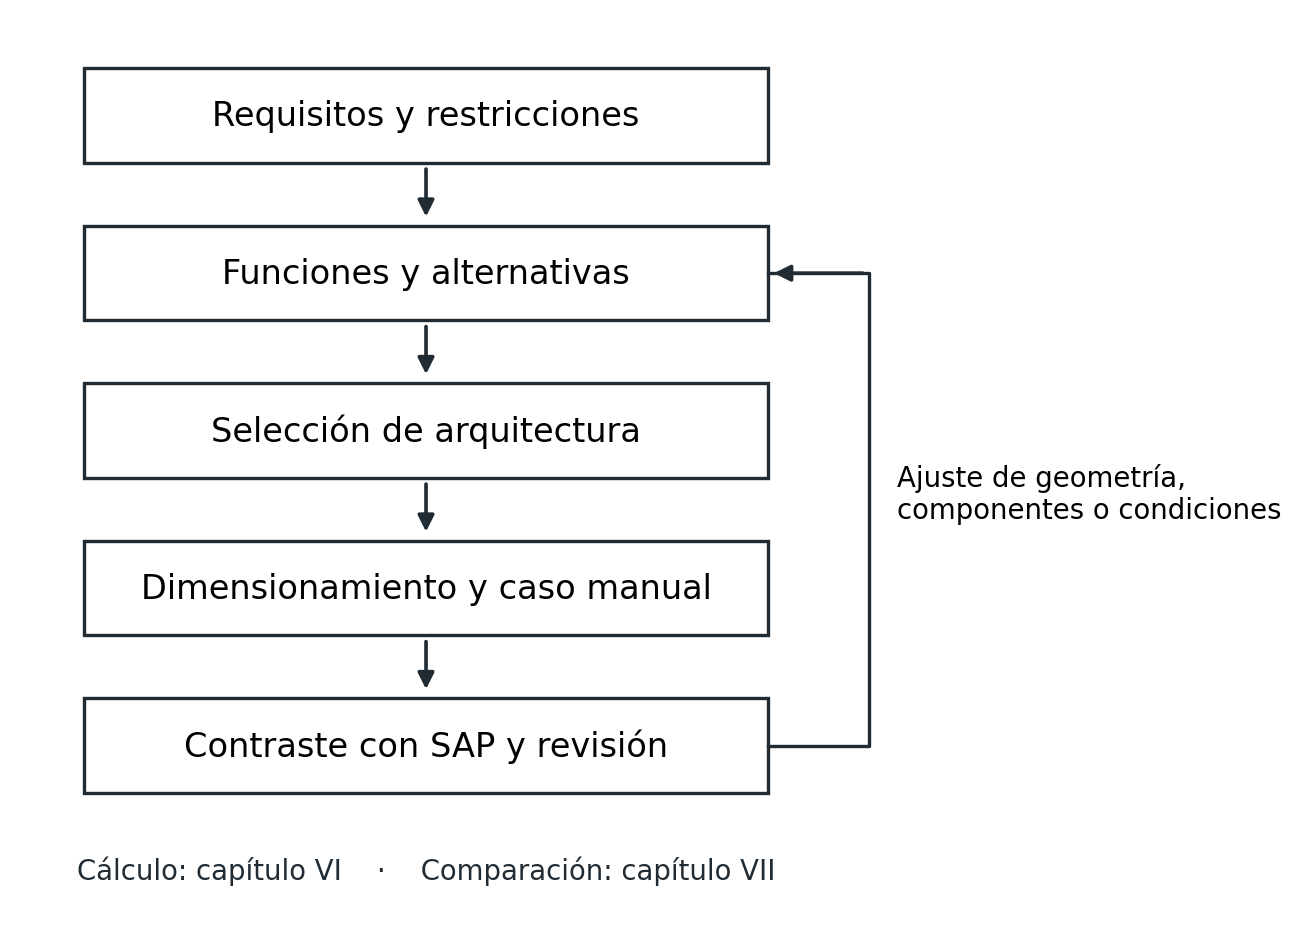
\includegraphics[width=0.93\textwidth]{images/proceso_metodologico}
\caption{Organización del proceso de diseño y retorno a las decisiones que requieren ajuste. Elaboración propia.}
\label{fig:metodo_revision}
\end{figure}

En el soporte se escogió un caso centrado con tres apoyos del rodamiento, cuyas reacciones verticales pueden obtenerse con las tres ecuaciones de equilibrio; ese desarrollo manual sirvió de control del modelo estructural. En la aspersión se definió una cadena que relaciona superficies objetivo, boquillas, caudal simultáneo, pérdidas del circuito y punto de bombeo, y que luego se contrastó con la simulación del mojado.

Las herramientas de modelado se eligieron según la pregunta que debía responder cada una. La Tabla~\ref{tab:herramientas} justifica cada herramienta e indica la verificación que se le aplicó.

\begingroup
\small\singlespacing
\setlength{\parskip}{0pt}
\setlength{\tabcolsep}{4pt}
\renewcommand{\arraystretch}{1.1}
\begin{longtable}{@{}>{\raggedright\arraybackslash}p{2.7cm}>{\raggedright\arraybackslash}p{\dimexpr(\textwidth-2.7cm-6\tabcolsep)/3\relax}>{\raggedright\arraybackslash}p{\dimexpr(\textwidth-2.7cm-6\tabcolsep)/3\relax}>{\raggedright\arraybackslash}p{\dimexpr(\textwidth-2.7cm-6\tabcolsep)/3\relax}@{}}
\caption{Herramientas de modelado, necesidad que atienden y verificación aplicada}\label{tab:herramientas}\\
\toprule
\textbf{Herramienta} & \textbf{Necesidad} & \textbf{Justificación} & \textbf{Verificación}\\
\midrule\endfirsthead
\caption[]{Herramientas de modelado, necesidad que atienden y verificación aplicada (continuación)}\\
\toprule
\textbf{Herramienta} & \textbf{Necesidad} & \textbf{Justificación} & \textbf{Verificación}\\
\midrule\endhead
\midrule\multicolumn{4}{r}{\textit{Continúa en la página siguiente.}}\\\endfoot
\bottomrule\endlastfoot
SAP2000 24.2.0 y 27.1 & Respuesta global del bastidor de perfiles y del soporte superior del distribuidor. & Modelo de barras con comprobación AISC 360-16 \cite{csi_analisis_2016,aisc360}. & Equilibrio contrastado con el cálculo manual; tablas exportadas.\\
FreeCAD FEM, Gmsh y CalculiX & Flexión local de los soportes de los centradores, que un modelo de barras no capta. & Elementos sólidos sobre la geometría real del perfil y las placas \cite{shigley2015}. & Dos niveles de malla, ambos signos de carga y control de equilibrio.\\
CalculiX y parrilla de pared delgada en Python & Torsión del bastidor de perfiles abiertos; el modelo de barras solo representa la torsión uniforme. & Torsión no uniforme con alabeo \cite{aiscdg9}. & Casos de control analíticos y cálculo independiente.\\
Guiones en Python & Red hidráulica iterativa, trazado de rayos y posproceso del CFD. & Cálculo reproducible y trazable. & Reproducción exacta del caso de cálculo manual.\\
ANSYS Fluent 2026 R1 & Mojado y dosis de la configuración base de 22 boquillas y de la configuración inferior de 24 boquillas. & Fase discreta lagrangiana acoplada al aire \cite{fluent2026}. & Tres mallas, paso de tiempo, dominio, número de parcelas y caso puente.\\
OpenFOAM v2606 & Mojado del agujero con las boquillas de la lanza; impacto local de una lámina con volumen de fluido (interFoam). & Mismo modelo físico en código abierto; volumen de fluido para la película \cite{deshpande2012}. & Caso puente con Fluent; cuatro mallas en el impacto local.\\
FreeCAD 1.1 (CAD) & Geometría, masas, interferencias y barridos del conjunto. & Modelo paramétrico regenerable por guiones. & Barridos de traslado, giro, retirada de la lanza y accionamiento; auditoría de solapes.\\
SolidWorks 2024 & Planos normalizados, detección de interferencias y verificaciones locales de piezas. & Herramienta de dibujo con símbolos ISO de soldadura y estudios estáticos de sólidos. & Cotas contrastadas con el CAD; segunda revisión de interferencias.\\
\end{longtable}
\endgroup

El CFD se ejecutó en ANSYS Fluent. Antes de ampliar el dominio se repitió en Fluent el caso del agujero ya resuelto en OpenFOAM; ese caso puente permitió comprobar que el cambio de programa no alteraba el resultado en esa superficie (Sección~\ref{sec:resultados-aspersion}). Las simulaciones de Fluent las ejecutó el segundo autor.

\paragraph{Uso de herramientas de inteligencia artificial.} Se usaron asistentes basados en inteligencia artificial en cuatro tareas. La primera fue programar guiones de cálculo y de posproceso, y guiones que generaron por interfaz de programación los modelos de SAP2000, el modelo CAD en FreeCAD y los planos en SolidWorks. La segunda fue revisar de forma independiente cálculos y la coherencia de los datos entre archivos. La tercera fue proponer alternativas de diseño, que los autores decidieron o confirmaron. La cuarta fue preparar borradores de texto y de tablas de este informe a partir de los archivos del proyecto. Los autores definieron el problema y los criterios, tomaron las decisiones de diseño y son responsables del contenido. Los guiones y sus salidas se conservan en el Anexo~\ref{anx:programas}, de modo que cada resultado puede reproducirse sin el asistente.

La estrategia de validación se basó en la verificación numérica de cada modelo (equilibrio, convergencia de malla, paso de tiempo y dominio) y en el contraste cruzado entre métodos independientes, cuyos escenarios se desarrollan en la Sección~\ref{sec:plan-pruebas}. Cada resultado se verificó por simulación o por cálculo; ninguno se validó con ensayos. La comprobación experimental de la huella de la boquilla, de la remoción del contaminante, del traslado y del bloqueo queda fuera del alcance de la tesis.

\section{Formulación de especificaciones técnicas}

Las necesidades se tradujeron en dimensiones, cargas, condiciones funcionales y criterios de aceptación. Se distinguieron los datos impuestos por el rodamiento, los criterios adoptados por el proyecto y las metas propuestas para el subsistema de limpieza. Las dimensiones de un perfil o la ubicación final de un mecanismo no se trataron como necesidades del usuario, pues corresponden a decisiones que se justifican durante el dimensionamiento.

Las metas del subsistema de aspersión E09--E13 proceden de la especificación de requerimientos que el equipo elaboró a partir de la reunión técnica con la empresa de remanufactura de referencia. Esa especificación se redactó para una arquitectura anterior del aplicador, por lo que se conservaron solo los requisitos funcionales y de desempeño que no dependen de ella. La Tabla~\ref{tab:especificaciones_revision} asigna a cada especificación su origen, su estado y su método de comprobación.

\begingroup
\small\singlespacing
\setlength{\parskip}{0pt}
\setlength{\tabcolsep}{4pt}
\renewcommand{\arraystretch}{1.1}
\begin{longtable}{@{}>{\raggedright\arraybackslash}p{1.0cm}>{\raggedright\arraybackslash}p{\dimexpr(\textwidth-1.0cm-6\tabcolsep)*40/100\relax}>{\raggedright\arraybackslash}p{\dimexpr(\textwidth-1.0cm-6\tabcolsep)*25/100\relax}>{\raggedright\arraybackslash}p{\dimexpr(\textwidth-1.0cm-6\tabcolsep)*35/100\relax}@{}}
\caption{Especificaciones técnicas, origen y método de comprobación}\label{tab:especificaciones_revision}\\
\toprule
\textbf{Cód.} & \textbf{Requisito o meta} & \textbf{Origen y estado} & \textbf{Método de comprobación}\\
\midrule\endfirsthead
\caption[]{Especificaciones técnicas, origen y método de comprobación (continuación)}\\
\toprule
\textbf{Cód.} & \textbf{Requisito o meta} & \textbf{Origen y estado} & \textbf{Método de comprobación}\\
\midrule\endhead
\midrule\multicolumn{4}{r}{\textit{Continúa en la página siguiente.}}\\\endfoot
\bottomrule\endlastfoot
\multicolumn{4}{@{}l}{\textit{Soporte y posicionamiento}}\\
E01 & Admitir el rodamiento de diámetro exterior 1420 mm, agujero de 900 mm y ancho de 515 mm. & Ficha del fabricante \cite{skf241}. & Envolvente de la pieza en el modelo.\\
E02 & Recibir una masa de rodamiento de 3032 kg y considerar por separado los pesos de estructura y accesorios. & Ficha del fabricante. & Balance de masas y correspondencia con las cargas de cada cálculo.\\
E03 & Mantener la flecha relativa del miembro evaluado dentro de $L/800$. & Criterio propuesto; L/360 y L/1000 se informan como referencia. & Desplazamiento respecto de la cuerda de sus extremos.\\
E04 & Relación demanda/capacidad no mayor que uno bajo las combinaciones declaradas. & AISC 360-16 \cite{aisc360}. & Resumen de diseño de acero; uniones por separado.\\
E05 & Transmitir reacciones normales compresivas en las interfaces sin amarre vertical. & Condición física del contacto. & Equilibrio y factibilidad del contacto.\\
E06 & Error radial de colocación del rodamiento no mayor que 5 mm. & Criterio del proyecto. & Presupuesto de tolerancias sobre el modelo, por nivel de fuerza del centrador.\\
E07 & Permitir la carga exterior y mantener la mesa inmovilizada durante el lavado. & Requisito funcional. & Envolventes de movimiento, bloqueo y secuencia.\\
E08 & Carrera de captura del centrador no menor que 5 mm después de tolerancias, con excentricidad inicial de 5 mm en cualquier dirección. & Criterio del proyecto. & Barridos de captura y presupuesto de tolerancias.\\
\multicolumn{4}{@{}l}{\textit{Aplicación del fluido}}\\
E09 & Presión en la toma de cada boquilla entre 4 y 6 bar (admisible entre 2 y 8 bar). & Especificación del subsistema de aspersión. & Red hidráulica.\\
E10 & Presión de aplicación no mayor que 8 bar, para preservar las pistas. & Especificación del subsistema de aspersión. & Red hidráulica.\\
E11 & Velocidad en la tubería de impulsión entre 1 y 3 m/s. & Especificación del subsistema de aspersión. & Red hidráulica.\\
E12 & Velocidad del rotor entre 1 y 2 rpm (admisible entre 0,5 y 5 rpm) y tiempo por vuelta entre 30 y 60 s. & Especificación del subsistema de aspersión. & Valor de operación del aplicador.\\
E13 & Cobertura geométrica de las superficies exteriores y del agujero de al menos 80\,\% (mínimo) y 95\,\% (objetivo). & Especificación del subsistema de aspersión. & Trazado de rayos y CFD.\\
\multicolumn{4}{@{}l}{\textit{Integración}}\\
E14 & Holgura positiva entre la mesa y el aplicador en traslado y giro. & Requisito funcional. & Barridos CAD.\\
\end{longtable}
\endgroup

Todas las especificaciones se comprueban por cálculo, simulación o modelo CAD, que es el alcance de la tesis. El modelo de mojado mide el líquido que llega a cada superficie y no el desprendimiento de la grasa, por lo que la especificación del subsistema no incluye metas de remoción.

\section{Descripción técnica de múltiples restricciones realistas}
\label{sec:filtros-diseno}

Las restricciones RS-01--RS-12 del Capítulo~\ref{cap:marco-referencial} se convirtieron en reglas de admisión para las alternativas. Un concepto que incumpla una condición indispensable no puede compensar ese incumplimiento con una nota alta en costo o simplicidad. Cuando falta el dato necesario para aplicar un filtro, la decisión se conserva abierta hasta disponer de la evidencia correspondiente. No se estableció como exclusión general el giro del rodamiento: las arquitecturas con giro se conservaron para compararlas, siempre que incorporaran soporte, sujeción y protección compatibles con la masa.

La Tabla~\ref{tab:filtros_revision} muestra la regla de admisión de cada restricción y su resultado para las cuatro alternativas.

\begingroup
\small\singlespacing
\setlength{\parskip}{0pt}
\setlength{\tabcolsep}{4pt}
\renewcommand{\arraystretch}{1.1}
\begin{longtable}{@{}>{\raggedright\arraybackslash}p{2.3cm}>{\raggedright\arraybackslash}p{\dimexpr(\textwidth-2.3cm-4\tabcolsep)*55/100\relax}>{\raggedright\arraybackslash}p{\dimexpr(\textwidth-2.3cm-4\tabcolsep)*45/100\relax}@{}}
\caption{Aplicación de restricciones como filtros de diseño}\label{tab:filtros_revision}\\
\toprule
\textbf{Restricción} & \textbf{Regla de admisión} & \textbf{Resultado para A1--A4}\\
\midrule\endfirsthead
\caption[]{Aplicación de restricciones como filtros de diseño (continuación)}\\
\toprule
\textbf{Restricción} & \textbf{Regla de admisión} & \textbf{Resultado para A1--A4}\\
\midrule\endhead
\midrule\multicolumn{3}{r}{\textit{Continúa en la página siguiente.}}\\\endfoot
\bottomrule\endlastfoot
RS-02 Masa y geometría & Se excluye la configuración que no admite la carga o la envolvente requeridas. & Pasan las cuatro; A1 y A4 condicionadas a una sujeción para giro compatible con 3032 kg.\\
RS-03 Preservación y acceso & Se modifica o excluye el concepto que obstruye una zona requerida o transmite carga por una superficie no prevista. & Pasan las cuatro a nivel funcional; la cobertura se verifica en el Capítulo~\ref{cap:resultados}.\\
RS-04--RS-05 Izaje, espacio y losa & Se excluye una disposición con interferencia; sin levantamiento de planta, la aptitud final depende de ese dato. & Condicionadas para las cuatro (requieren datos de planta).\\
RS-01, RS-11 Movimiento y bloqueo & Se excluye una secuencia que requiere lavar con la mesa sin inmovilizar o intervenir en una zona de movimiento peligroso. & Pasan las cuatro con inmovilización durante el lavado.\\
RS-08--RS-09 Contención y fluido & Se excluye una propuesta cuya operación depende de descargar el fluido sin una gestión definida. & Pasan las cuatro con cabina, bandeja y recolección.\\
RS-10 Recursos económicos & Un presupuesto máximo se aplica como filtro solo si está documentado. & No aplicado como filtro (sin techo acreditado); el costo es criterio comparativo.\\
\end{longtable}
\endgroup

La aplicación de estos filtros distinguió una incompatibilidad demostrada de una selección que exige completar datos. Una capacidad publicada inferior a la masa de la pieza permitió descartar esa versión de equipo en el Capítulo~\ref{cap:estado-arte}; en cambio, la ausencia de una cotización no demuestra que una arquitectura sea inviable, solo impide cerrar su evaluación económica.

\section{Generación y selección de alternativas mediante matriz de decisión}

\subsection{Generación de alternativas}

El análisis funcional partió de cinco acciones: recibir el rodamiento, sostenerlo y posicionarlo, exponer sus superficies al medio de limpieza, aplicar el fluido y recoger el residuo. Se distinguió el movimiento necesario para cargar la máquina del movimiento utilizado durante el lavado. Esta separación evitó interpretar una pieza inmóvil durante la limpieza como una mesa que no puede salir de la cabina.

La Tabla~\ref{tab:morfologica_revision} organiza los principios de solución considerados. Las opciones de cada fila representan formas de realizar una función; su combinación se revisó para obtener máquinas completas y evitar conjuntos incompatibles.

\begingroup
\small\singlespacing
\setlength{\parskip}{0pt}
\setlength{\tabcolsep}{4pt}
\renewcommand{\arraystretch}{1.1}
\begin{longtable}{@{}>{\raggedright\arraybackslash}p{2.6cm}>{\raggedright\arraybackslash}p{\dimexpr(\textwidth-2.6cm-6\tabcolsep)/3\relax}>{\raggedright\arraybackslash}p{\dimexpr(\textwidth-2.6cm-6\tabcolsep)/3\relax}>{\raggedright\arraybackslash}p{\dimexpr(\textwidth-2.6cm-6\tabcolsep)/3\relax}@{}}
\caption{Principios de solución utilizados para generar alternativas}\label{tab:morfologica_revision}\\
\toprule
\textbf{Función} & \textbf{Opción 1} & \textbf{Opción 2} & \textbf{Opción 3}\\
\midrule\endfirsthead
\caption[]{Principios de solución utilizados para generar alternativas (continuación)}\\
\toprule
\textbf{Función} & \textbf{Opción 1} & \textbf{Opción 2} & \textbf{Opción 3}\\
\midrule\endhead
\midrule\multicolumn{4}{r}{\textit{Continúa en la página siguiente.}}\\\endfoot
\bottomrule\endlastfoot
Recibir la pieza & Carga por grúa sobre soporte accesible & Carro extraíble para carga exterior & Útil o canastilla compatible con la pieza\\
Exponer superficies & Giro de la pieza & Movimiento del aplicador & Aplicación desde posiciones distribuidas\\
Aplicar el fluido & Boquillas fijas & Aplicador móvil & Boquillas orientables\\
Sostener y localizar & Apoyos definidos y centradores & Plataforma con sujeción para giro & Útil de apoyo dedicado\\
Recoger el residuo & Cabina, bandeja y drenaje & La misma contención con retorno definido & Almacenamiento para gestión posterior\\
\end{longtable}
\endgroup

Se mantuvieron cuatro arquitecturas para la comparación. A1 utiliza una plataforma giratoria con boquillas fijas. A2 conserva el rodamiento inmóvil durante el lavado y mueve el aplicador alrededor de la pieza. A3 distribuye boquillas alrededor de la pieza sin accionar su masa. A4 combina giro limitado con orientación de las boquillas. Todas requieren una solución de carga y contención. La Figura~\ref{fig:alternativas_revision} representa únicamente el movimiento de limpieza de cada alternativa.

\begin{figure}[htbp]
\centering
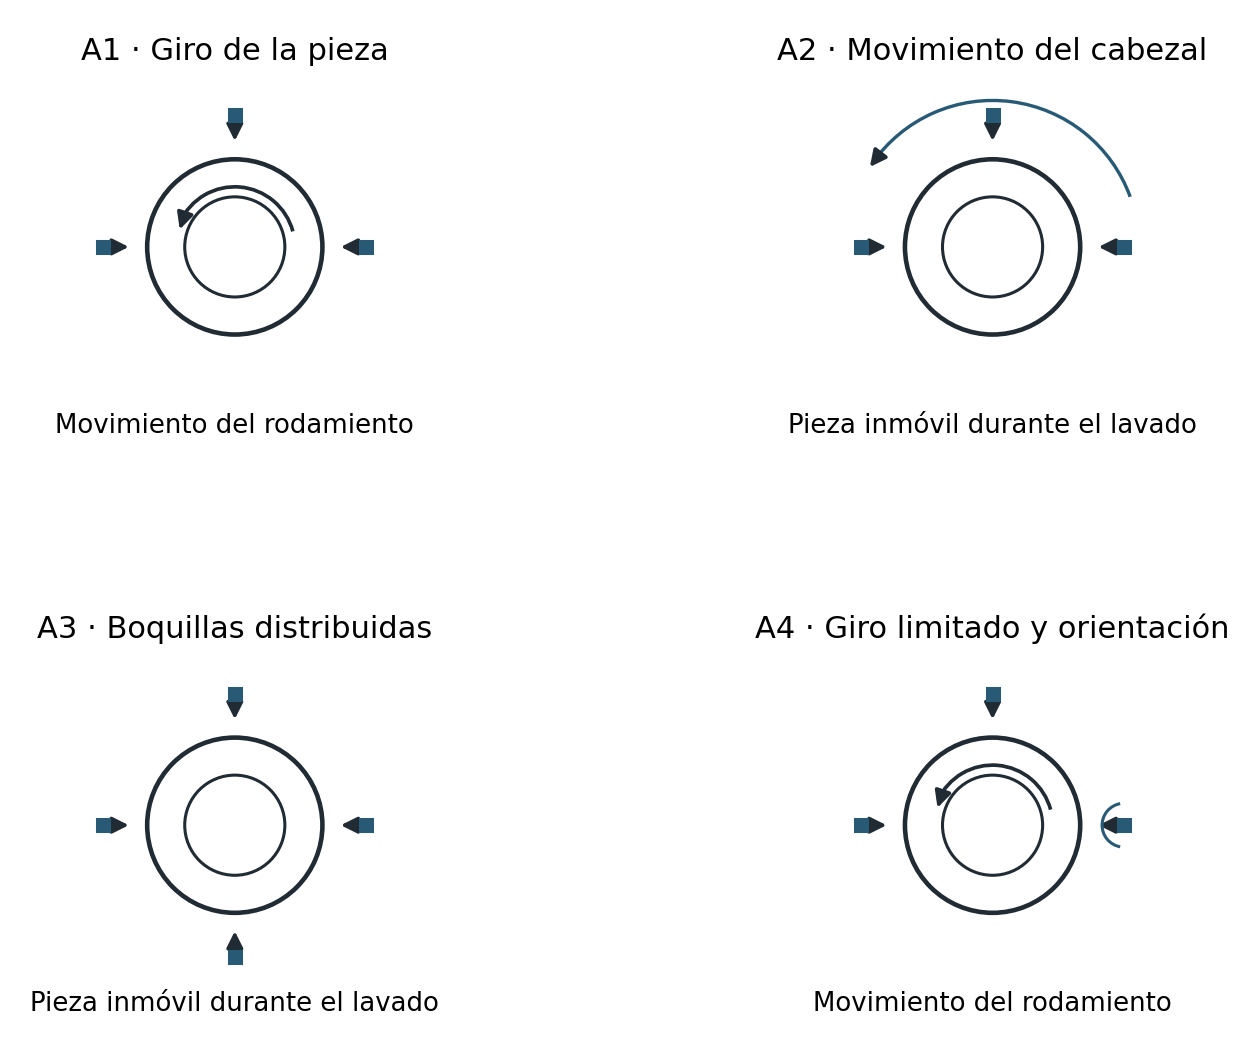
\includegraphics[width=0.94\textwidth]{images/alternativas_funcionales}
\caption{Principios de movimiento de las cuatro alternativas conceptuales. Elaboración propia.}
\label{fig:alternativas_revision}
\end{figure}

\subsection{Selección y trade-offs}

Las alternativas se compararon con una matriz de ocho criterios, pesos que suman uno y una escala de uno (condición desfavorable) a cuatro (muy favorable). Las notas expresan juicios de diseño basados en las funciones previstas; no equivalen a eficiencias medidas ni a probabilidades de falla. La seguridad recibió el mayor peso por la masa manipulada; la cobertura y la preservación, por su relación con la finalidad del lavado; energía y fluido, por las necesidades de accionamiento y aplicación; y fabricabilidad, mantenimiento y costo representaron la implementación. La Tabla~\ref{tab:matriz_revision} contiene las notas y el puntaje ponderado de cada alternativa.

\begin{table}[htbp]
\centering\small\singlespacing
\caption{Matriz ponderada de selección de la arquitectura}
\label{tab:matriz_revision}
\begin{tabular}{lccccc}
\toprule
\textbf{Criterio} & \textbf{Peso} & \textbf{A1} & \textbf{A2} & \textbf{A3} & \textbf{A4}\\
\midrule
Seguridad & 0,20 & 2 & 4 & 3 & 3\\
Cobertura & 0,17 & 3 & 4 & 3 & 4\\
Preservación & 0,15 & 2 & 4 & 4 & 3\\
Energía & 0,11 & 1 & 4 & 4 & 2\\
Fluido & 0,10 & 3 & 3 & 2 & 3\\
Fabricabilidad & 0,10 & 3 & 3 & 4 & 2\\
Mantenimiento & 0,09 & 3 & 3 & 4 & 2\\
Costo & 0,08 & 2 & 3 & 3 & 2\\
\midrule
\textbf{Resultado} & \textbf{1,00} & \textbf{2,35} & \textbf{3,63} & \textbf{3,35} & \textbf{2,79}\\
\bottomrule
\end{tabular}
\par\smallskip\footnotesize
Fuente: matriz de la etapa anterior del proyecto; se reproduce su cálculo. La nota de cobertura de A2 evalúa el alcance funcional del principio (superficies exteriores, caras y agujero con la pieza inmóvil), no una geometría concreta del aplicador.
\end{table}

El puntaje de cada alternativa se obtuvo multiplicando la nota de cada criterio por su peso y sumando los productos. Para A2, el cálculo fue
\[
\begin{aligned}
S_{A2}={}&0{,}20(4)+0{,}17(4)+0{,}15(4)+0{,}11(4)\\
&+0{,}10(3)+0{,}10(3)+0{,}09(3)+0{,}08(3)=3{,}63.
\end{aligned}
\]
Este resultado seleccionó A2 como arquitectura de desarrollo: el rodamiento permanece inmovilizado durante la aplicación del fluido y el aplicador realiza el movimiento de limpieza.

La comparación más cercana fue con A3. A2 obtuvo una ventaja de 0,28 puntos: sus mayores notas de seguridad, cobertura y uso de fluido aportaron 0,47 puntos, mientras que sus menores notas de fabricabilidad y mantenimiento descontaron 0,19. El compromiso consistió en aceptar un mecanismo de accionamiento del aplicador a cambio de no mover una masa de tres toneladas y de variar la trayectoria de las boquillas alrededor de la pieza. Como A2 y A3 recibieron la misma nota de costo, aumentar únicamente ese peso no invierte su orden, aunque reduce la distancia entre sus puntajes.

La materialización del principio A2 evolucionó durante el desarrollo: de un aplicador anular con lanza axial a un cabezal sobre monorriel y, finalmente, a una U superior giratoria con una lanza interior y un par de boquillas inferiores en cada brazo (Anexo~\ref{anx:iteraciones}). La misma lógica de decisión se aplicó en un segundo nivel al número de apoyos del bastidor (Anexo~\ref{anx:iteraciones}), al mecanismo de centrado (Sección~\ref{sec:seleccion-componentes}), al sistema de traslado y a la rueda (Sección~\ref{sec:seleccion-traslado-rueda}).

\subsection{Selección del sistema de traslado y de la rueda}
\label{sec:seleccion-traslado-rueda}

El traslado de la mesa cargada se planteó primero como empuje manual. Con la masa de diseño de 3500~kg, el empuje calculado fue de 325~N para arrancar en el escenario de diseño y de 837~N en el adverso, y la parada en 0,10~m exigía 565~N (Sección~\ref{sec:dimensionamiento-traslado}). Esas fuerzas superan la cifra guía de la HSE británica para iniciar o detener a mano una carga empujada, 200~N para hombres y 150~N para mujeres, que es un filtro de riesgo y no un límite \cite{hsepushpull}. Por eso el empuje directo, incluso con un freno, no pasó el filtro de ergonomía. Las demás opciones se compararon en una matriz ponderada que incluyó la disponibilidad de componentes en el mercado local (Tabla~\ref{tab:traslado-alternativas}).

\begin{table}[htbp]
\centering\small\singlespacing
\caption{Selección del sistema de traslado de la mesa}
\label{tab:traslado-alternativas}
\begin{tabularx}{\textwidth}{@{}Ycccccc>{\bfseries}c@{}}
\toprule
\textbf{Alternativa} & \textbf{Seg.} & \textbf{Conf.} & \textbf{Costo} & \textbf{Integr.} & \textbf{Oper.} & \textbf{Disp.} & \textbf{Total}\\
 & 0,25 & 0,20 & 0,20 & 0,15 & 0,10 & 0,10 & \\
\midrule
Empuje manual con freno & \multicolumn{7}{c}{No pasa el filtro: 325--837~N frente a 200~N} \\
Manivela en la mesa, rueda motriz & 4 & 3 & 4 & 2 & 3 & 4 & 3,40\\
Motorreductor en la mesa, rueda motriz & 4 & 2 & 2 & 1 & 5 & 3 & 2,75\\
Cable sin fin con motor fijo & 4 & 3 & 2 & 3 & 5 & 3 & 3,25\\
Cable sin fin con torno manual & 4 & 3 & 4 & 3 & 2 & 4 & 3,45\\
Doble cadena bajo la mesa, motorizada & 4 & 4 & 2 & 4 & 5 & 4 & 3,70\\
Doble cadena bajo la mesa, con volante & 5 & 4 & 4 & 4 & 3 & 5 & 4,25\\
\bottomrule
\end{tabularx}
\par\smallskip\footnotesize
Seg.: seguridad y ergonomía; Conf.: confiabilidad en ambiente húmedo; Integr.: integración sin modificar la mesa, las ruedas ni la puerta; Oper.: rapidez y repetibilidad; Disp.: disponibilidad local de componentes y mantenimiento. Puntajes de 1 a 5 asignados por los autores.
\end{table}

Se seleccionó la doble cadena bajo la mesa accionada con un volante fuera de la cabina, con 4,25 puntos. La segunda opción fue la misma cadena con motor, con 3,70. La diferencia está en el costo y la disponibilidad, a cambio de una operación más lenta: si el peso de la operación sube a 0,30, las dos cadenas empatan (3,99 y 3,97). Por ese resultado, la motorización se mantiene como mejora sobre la misma transmisión y se trata en las recomendaciones.

La rueda se revisó porque la versión anterior comparó la carga del estado límite último, de 26,62~kN, con la capacidad de rodadura a 4~km/h, de 24,52~kN, y obtuvo un exceso de 8,5\,\%. Esa capacidad corresponde al desgaste en servicio. Se separaron las dos comprobaciones y se compararon las ruedas de 200 y 250~mm del mismo fabricante (Tabla~\ref{tab:rueda-200-250}).

\begin{table}[htbp]
\centering\small\singlespacing
\caption{Comparación de las ruedas de 200 y 250 mm para la mesa de traslado}
\label{tab:rueda-200-250}
\begin{tabularx}{\textwidth}{@{}Yrr@{}}
\toprule
\textbf{Criterio} & \textbf{Rueda de 200 mm} & \textbf{Rueda de 250 mm}\\
\midrule
Capacidad de rodadura a 4~km/h \cite{blickle2026} & 24,52 kN & 39,23 kN\\
Capacidad estática \cite{blickle2026} & 61,29 kN & 98,07 kN\\
Servicio: 21,87 kN frente a la capacidad de rodadura & 0,89 & 0,56\\
Estado límite último: 26,62 kN frente a la capacidad estática & 0,43 & 0,27\\
Riel asignado y masa de los dos rieles \cite{arcelor2023} & A45; 289 kg & A55; 416 kg\\
Costo adicional respecto de la rueda de 200 mm & -- & S/~4230 (14\,\%)\\
Masa móvil adicional & -- & 56 kg\\
\bottomrule
\end{tabularx}
\par\smallskip\footnotesize
Rueda más cargada con la mesa en tres ruedas, masa de 3500~kg, excentricidad de 100~mm en ambas direcciones y factor de impacto de 1,15; la carga última aplica 1,40. El precio de la rueda de 250~mm se estimó por su masa.
\end{table}

Se mantuvo la rueda de 200~mm sobre riel A45. Cumple las dos comprobaciones con supuestos envolventes, mientras que la de 250~mm costaría unos S/~4230 más y obligaría a cambiar el riel, el eje y la horquilla. Falta que el fabricante confirme la capacidad a la velocidad de traslado de la mesa, muy inferior a los 4~km/h del catálogo.

\subsection{Criterios ambiental y social}
\label{sec:matriz-ambiental-social}

La matriz no separó criterios ambiental y social: sus efectos están en los criterios de fluido y energía, que miden el consumo y el efluente, y en el de seguridad, que mide la exposición del personal. El Capítulo~\ref{cap:seguridad-ambiente} los evalúa de forma cualitativa para la arquitectura seleccionada, de modo que el puntaje de A2 sustenta la arquitectura de desarrollo y no una comparación ambiental entre alternativas.

\section{Descripción general de los componentes o partes de la solución seleccionada}

La solución seleccionada realiza un lavado exterior del rodamiento completo, para su inspección visual, retirado del HPGR y apoyado horizontalmente con su eje vertical e inmóvil durante la aplicación del fluido, antes de desmontarlo por componentes. En esta primera etapa se tratan las superficies exteriores, las dos caras y la superficie accesible del agujero; no se busca limpiar los espacios internos entre rodillos y aros. La segunda etapa, conceptual y fuera del alcance de esta máquina, comprende la limpieza de los elementos desmontados (aros, rodillos y jaula) y de las zonas que el lavado no alcanza, como la franja que ocultan los topes de retención. Sus útiles y criterios de limpieza no se dimensionan ni evalúan en este proyecto.

El soporte es una mesa móvil con bastidor de perfiles W6$\times$9 que se extrae de la cabina para cargar el rodamiento con grúa. En la estación de carga se inserta el pasador de bloqueo y los centradores posicionan la pieza; luego una doble cadena accionada con un volante traslada la mesa sobre rieles hasta la estación de lavado, donde se bloquea de nuevo. Los tres apoyos sectoriales, a 0$^\circ$, 120$^\circ$ y 240$^\circ$ bajo la cara inferior del aro exterior, reciben la carga vertical; los centradores solo fijan la posición lateral y los topes retienen la pieza.

La aplicación se realiza con un distribuidor en U que gira a 1,7~rpm, alimentado por una unión rotativa y sostenido por un soporte superior, y con una lanza interior que entra por el agujero. En total hay 24 boquillas fijas: cada brazo de la U lleva dos superiores, cinco laterales y un par inferior de abanico estrecho, y la lanza lleva seis. La cabina contiene las salpicaduras y el líquido vuelve al tanque de lavado; el drenaje se representa en el esquema hidráulico, sin dimensionarse. La Tabla~\ref{tab:componentes_revision} relaciona cada conjunto con su función, el objetivo específico al que responde y la forma en que se dimensiona o verifica.

\begingroup
\small\singlespacing
\setlength{\parskip}{0pt}
\setlength{\tabcolsep}{4pt}
\renewcommand{\arraystretch}{1.1}
\begin{longtable}{@{}>{\raggedright\arraybackslash}p{2.8cm}>{\raggedright\arraybackslash}p{\dimexpr(\textwidth-2.8cm-6\tabcolsep)*38/100\relax}>{\raggedright\arraybackslash}p{\dimexpr(\textwidth-2.8cm-6\tabcolsep)*12/100\relax}>{\raggedright\arraybackslash}p{\dimexpr(\textwidth-2.8cm-6\tabcolsep)*50/100\relax}@{}}
\caption{Componentes de la solución seleccionada y su dimensionamiento}\label{tab:componentes_revision}\\
\toprule
\textbf{Conjunto} & \textbf{Función} & \textbf{OE} & \textbf{Dimensionamiento o verificación}\\
\midrule\endfirsthead
\caption[]{Componentes de la solución seleccionada y su dimensionamiento (continuación)}\\
\toprule
\textbf{Conjunto} & \textbf{Función} & \textbf{OE} & \textbf{Dimensionamiento o verificación}\\
\midrule\endhead
\midrule\multicolumn{4}{r}{\textit{Continúa en la página siguiente.}}\\\endfoot
\bottomrule\endlastfoot
Bastidor de perfiles & Recibir y transmitir las cargas. & OE4 & Modelo de barras, torsión no uniforme y uniones soldadas a momento.\\
Apoyos sectoriales y revestimiento & Apoyar el rodamiento y preservar la superficie de contacto. & OE4 & Reacciones por equilibrio y presión media.\\
Ruedas, rieles y pedestales & Rodar la mesa entre las estaciones de carga y lavado. & OE4 & Carga de rueda, fuerza lateral de guiado, viga del riel y anclajes.\\
Traslado por doble cadena & Mover y detener la mesa sin empuje directo. & OE3, OE4 & Matriz de selección, tiro de la cadena, eje y fuerza en el volante.\\
Centradores & Posicionar el rodamiento sin soportar su peso. & OE4, OE5 & Selección multicriterio, FEM local y error de colocación por nivel de fuerza.\\
Bloqueo y topes & Inmovilizar la mesa y retener la pieza. & OE4 & Pasador con ajuste H7/g6 y secuencia de operación.\\
Distribuidor en U, eje y cubo & Aplicar el fluido al exterior y a las dos caras. & OE4, OE5 & Huella, número de boquillas, CFD y verificación estructural.\\
Lanza interior & Aplicar el fluido al agujero y a la parte interior de la cara inferior. & OE4, OE5 & Visibilidad geométrica y CFD.\\
Soporte superior y accionamiento & Sostener el distribuidor y hacerlo girar con par limitado. & OE4 & Selección de catálogo y comprobaciones resumidas (Anexo~\ref{anx:calculos}).\\
Circuito hidráulico & Alimentar las 24 boquillas desde el tanque. & OE4 & Red iterativa, altura, potencia, NPSH y esquema hidráulico.\\
Cabina, tanques y drenaje & Contener, recoger y recircular el líquido. & OE4 & Representación en el CAD y en el esquema hidráulico, barridos y presupuesto; sin dimensionamiento.\\
\end{longtable}
\endgroup

El Capítulo~\ref{cap:diseno} desarrolla el dimensionamiento de cada conjunto con las ecuaciones del Capítulo~\ref{cap:marco-teorico}; el Capítulo~\ref{cap:resultados} somete el conjunto dimensionado a la verificación numérica frente a las especificaciones y las restricciones.

\chapter{DISEÑO TECNOLÓGICO}
\label{cap:diseno}

\section{Cálculo de los parámetros y dimensionamiento de los componentes}

\subsection{Bases de diseño}
\label{sec:bases-diseno}

El origen de coordenadas se ubica en el centro nominal del rodamiento en la estación de lavado. El eje $X$ es transversal a los rieles, $Y$ sigue el recorrido de la mesa y $Z$ es vertical, medido desde el piso de la cabina; las coordenadas se expresan en milímetros. La Tabla~\ref{tab:bases-diseno} reúne los datos y las hipótesis que gobiernan el dimensionamiento, con su procedencia y su estado. Las hipótesis se adoptaron para avanzar y se revisan cuando se disponga del dato que las reemplace.

\begingroup
\footnotesize\singlespacing
\setlength{\parskip}{0pt}
\setlength{\tabcolsep}{4pt}
\renewcommand{\arraystretch}{1.05}
\begin{longtable}{@{}>{\raggedright\arraybackslash}p{4.3cm}>{\raggedright\arraybackslash}p{3.4cm}>{\raggedright\arraybackslash}p{\dimexpr\textwidth-4.3cm-3.4cm-2.4cm-6\tabcolsep\relax}>{\raggedright\arraybackslash}p{2.4cm}@{}}
\caption{Bases de diseño y entradas del dimensionamiento}\label{tab:bases-diseno}\\
\toprule
\textbf{Parámetro} & \textbf{Valor} & \textbf{Procedencia} & \textbf{Estado}\\
\midrule\endfirsthead
\caption[]{Bases de diseño y entradas del dimensionamiento (continuación)}\\
\toprule
\textbf{Parámetro} & \textbf{Valor} & \textbf{Procedencia} & \textbf{Estado}\\
\midrule\endhead
\midrule\multicolumn{4}{r}{\textit{Continúa en la página siguiente.}}\\\endfoot
\bottomrule\endlastfoot
\multicolumn{4}{@{}l}{\textit{Rodamiento y soporte}}\\
Rodamiento SKF 241/900 ECAK30/W33 & Diámetro exterior 1420; agujero 900 (extremo menor del cono 1:30); ancho 515 mm & Ficha del fabricante \cite{skf241} & Dato\\
Masa del rodamiento & 3032 kg & Ficha del fabricante & Dato\\
Carga externa del modelo estructural & $3\times9948=29\,844$ N & Corrida estructural de referencia & Dato de la corrida\\
Masa móvil & 3439,8 kg por componentes; unos 3462 kg con los cambios del centrador y de las ruedas & Balance de masas del conjunto & Calculado; estimado\\
Masa móvil de diseño & 3500 kg & Escenario adoptado & Hipótesis\\
Centro de gravedad del conjunto & $(0;\,-4{,}6;\,1093{,}3)$ mm & Balance de masas & Calculado\\
Aceleración horizontal de traslado & 0,3 m/s$^2$ & Caso de diseño mecánico & Hipótesis\\
Factores de servicio y resistente & 1,15 y 1,40 & Traslado lento sobre juntas; combinación resistente & Hipótesis\\
Error radial de colocación & $\leq5$ mm & Especificación E06 & Criterio del proyecto\\
\multicolumn{4}{@{}l}{\textit{Aspersión}}\\
Fluido & Agua con detergente alcalino de baja espuma (7--15 g/L) a 62 $^\circ$C; $\rho=982{,}12$ kg/m$^3$, $\mu=4{,}523\times10^{-4}$ Pa\,s & Propiedades del agua \cite{bell2014}; detergente \cite{zep36342} & Fluido base de cálculo\\
Presión mínima en la boquilla más desfavorable & 4 bar & Criterio de diseño (dentro de E09) & Criterio adoptado\\
Boquillas & Abanico plano H3/8U-316SS5020 (50$^\circ$) y H3/8U-316SS1520 (15$^\circ$): 2 gal/min a 40 psi & Catálogo \cite{manSpray} & Candidatas\\
Solape mínimo entre huellas & 25\,\% & Criterio geométrico & Criterio adoptado\\
Coeficiente de velocidad de la boquilla & $C_v=0{,}95$ & Valor supuesto & Hipótesis\\
Tubería & DN15, DN25, DN40 y DN50 Sch10S; $\varepsilon=0{,}045$ mm & ASME B36.19M \cite{asmeb3619} & Dato normalizado; rugosidad supuesta\\
Coeficientes de accesorios & $K=n f_T$ & Método de Crane \cite{crane410} & Método adoptado\\
Pérdidas en unión rotativa y filtro & 0,30 y 0,20 bar & Valores supuestos & Hipótesis\\
Eficiencias de bomba y motor & 0,55 y 0,85 & Valores supuestos & Hipótesis\\
Altitud del sitio & 2335 m & Escenario de cálculo (Arequipa) & Hipótesis de sitio\\
Giro del distribuidor & 1,7 rpm & Estudio analítico previo de aspersión & Hipótesis de operación\\
Conjunto giratorio con agua & 231 kg; centro de gravedad a 79,6 mm del eje & Masa medida en el modelo CAD & Calculado\\
\end{longtable}
\endgroup

\subsection{Subsistema de soporte}
\label{sec:dimensionamiento-soporte}

\subsubsection{Geometría del bastidor}

El bastidor está formado por siete barras de perfil W6$\times$9 de acero ASTM A36 con las alas superiores en un mismo plano: dos vigas longitudinales en $X=\pm930$ mm, dos testeros en $Y=\pm950$ mm, dos travesaños de carga en $Y=\pm574{,}175$ mm y una viga central bajo el apoyo A en $X=663$ mm. Sus líneas medias abarcan $1860\times1900$ mm. Los tres apoyos sectoriales se ubican sobre un radio nominal de 663 mm y las cuatro ruedas, en $(\pm930;\,\pm722)$ mm, bajo las almas de las vigas longitudinales, de modo que no se requieren ménsulas en voladizo (Tabla~\ref{tab:coordenadas-soporte}). La planta del bastidor está en el plano del Anexo~\ref{anx:planos}.

\begin{table}[htbp]
\centering\small\singlespacing
\caption{Posiciones de apoyos y ruedas en el cálculo de equilibrio}
\label{tab:coordenadas-soporte}
\begin{tabular}{lrrl}
\toprule
\textbf{Elemento} & \textbf{$X$ (mm)} & \textbf{$Y$ (mm)} & \textbf{Nodo del modelo}\\
\midrule
Apoyo A & 663,0 & 0,0 & 10\\
Apoyo B & $-331,5$ & 574,2 & 8\\
Apoyo C & $-331,5$ & $-574,2$ & 7\\
Ruedas 1 y 2 & $-930,0$ & $\mp722,0$ & 2 y 5\\
Ruedas 3 y 4 & 930,0 & $\mp722,0$ & 13 y 16\\
\bottomrule
\end{tabular}
\end{table}

\subsubsection{Equilibrio del rodamiento sobre los apoyos sectoriales}

El rodamiento se idealizó como un cuerpo apoyado en tres puntos no colineales con reacciones verticales; con la Ecuación~\eqref{eq:teo-reparto} y las coordenadas de la Tabla~\ref{tab:coordenadas-soporte}, el sistema queda determinado:
\begin{equation}
\begin{bmatrix}
1&1&1\\
663&-331{,}5&-331{,}5\\
0&574{,}18&-574{,}18
\end{bmatrix}
\begin{bmatrix}R_A\\R_B\\R_C\end{bmatrix}
=
\begin{bmatrix}W_r\\W_r x_r\\W_r y_r\end{bmatrix}.
\label{eq:dis-reparto-pad}
\end{equation}
Para la resultante centrada ($x_r=y_r=0$) y $W_r=29\,844$ N se obtuvo $R_A=R_B=R_C=9948$ N. Las tres reacciones son compresivas, de modo que la hipótesis de contacto cerrado es admisible. Con el área de revestimiento de un sector de $24^\circ$ entre los radios 638 y 688 mm, $A=13\,886$ mm$^2$, la presión media nominal resultó
\begin{equation}
p_m=\frac{R}{A}=\frac{9948}{13\,886}=0{,}716\ \mathrm{MPa}.
\label{eq:dis-presion-pad}
\end{equation}
Con la masa de diseño, el error de colocación de 5 mm y la excentricidad inercial equivalente de 7,9 mm, la envolvente analítica dio 11,85 kN por apoyo en servicio y 14,42 kN en condición resistente, con presiones medias de 0,853 y 1,038 MPa. La presión media no representa el máximo local del contacto; la admisibilidad del revestimiento de polietileno de ultra alto peso molecular requiere su resistencia a compresión sostenida a la temperatura de operación, que el fabricante debe confirmar. El desarrollo completo y el contraste con el modelo estructural están en la Sección~\ref{sec:memoria-soporte} del Anexo~\ref{anx:calculos}.

\subsubsection{Uniones soldadas del bastidor}
\label{sec:uniones-bastidor}

El modelo global del bastidor mostró que la rigidez bajo las cargas de centrado depende de que los nudos transmitan momento y alabeo (Sección~\ref{sec:resultados-soporte}). Por eso se diseñaron las diez uniones a momento: cuatro de viga longitudinal con travesaño de carga, dos de travesaño con viga central y cuatro esquinas. El detalle es el mismo en todas:
\begin{itemize}
\item la barra que llega lleva destaje de alas, y sus alas se sueldan a tope con penetración completa contra el canto de las alas de la barra continua, de modo que forman una sola placa en el nudo;
\item el alma lleva un filete de 3 mm por ambos lados;
\item la barra continua lleva un rigidizador de 6 mm en el lado opuesto, que impide la distorsión de la sección;
\item las esquinas se cierran con una tapa de 6 mm soldada en todo el contorno, que además sella la rendija frente al agua alcalina.
\end{itemize}

Las fuerzas en los nudos se obtuvieron con una parrilla de barras con alabeo, contrastada con SAP2000: el momento máximo de la viga central dio 4,008 kN\,m frente a 4,014 kN\,m ($-0{,}1$\,\%). Se revisaron los casos de centrado y de lavado y dos casos que el modelo estructural anterior no tenía: el desvío lateral de una rueda durante el traslado, con 6,51 kN en el contacto, y el tiro de las cadenas. Cada unión se verificó con la Ecuación~\eqref{eq:mt-filete} y las disposiciones de AISC 360-16 \cite{aisc360}. La Tabla~\ref{tab:uniones-bastidor} resume los resultados y la Figura~\ref{fig:plano-uniones}, el detalle del plano.

\begin{table}[htbp]
\centering\small\singlespacing
\caption{Verificación de las uniones soldadas y de las barras del bastidor}
\label{tab:uniones-bastidor}
\begin{tabularx}{\textwidth}{@{}YcYrr@{}}
\toprule
\textbf{Unión o barra} & \textbf{Cant.} & \textbf{Caso que gobierna} & \multicolumn{2}{c}{\textbf{D/C}}\\
\cmidrule(l){4-5}
 & & & \textbf{Alas} & \textbf{Alma}\\
\midrule
Viga longitudinal con travesaño de carga & 4 & Desvío lateral de una rueda & 0,30--0,58 & 0,15\\
Travesaño de carga con viga central & 2 & Centrado, disparo del limitador & 0,14 & 0,09\\
Esquina: viga longitudinal con testero & 4 & Desvío lateral; tiro de las cadenas & 0,21--0,28 & 0,02\\
\midrule
\multicolumn{5}{@{}l}{\textit{Barras completas, con las cargas del traslado}}\\
Vigas longitudinales & 2 & Desvío lateral de una rueda & \multicolumn{2}{r}{0,82}\\
Travesaños de carga & 2 & Desvío lateral y centrado & \multicolumn{2}{r}{0,58}\\
Testeros y viga central & 3 & -- & \multicolumn{2}{r}{$\leq0{,}26$}\\
\bottomrule
\end{tabularx}
\end{table}

\begin{figure}[htbp]
\centering
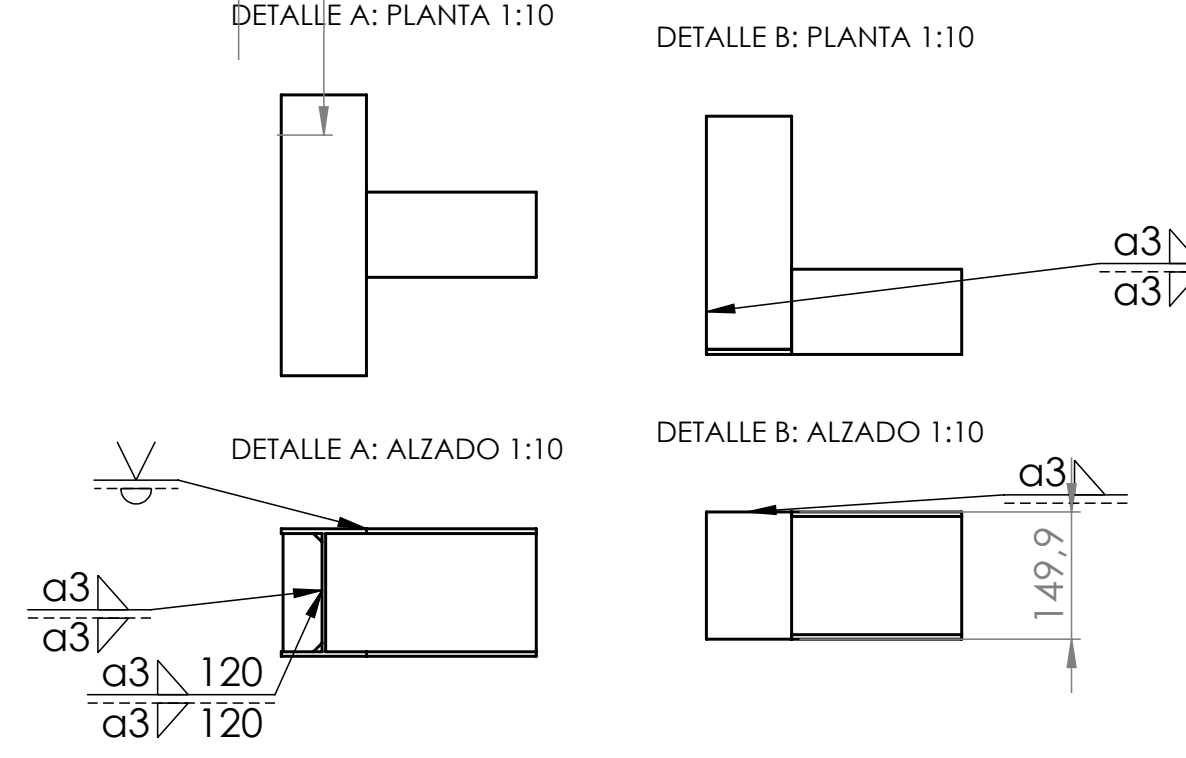
\includegraphics[width=0.80\textwidth]{plano_detalles_uniones.png}
\caption{Detalles del nudo en T (A) y de la esquina (B) del plano del bastidor, con los símbolos de soldadura ISO 2553 \cite{iso2553}. El plano completo está en el Anexo~\ref{anx:planos}. Elaboración propia en SolidWorks.}
\label{fig:plano-uniones}
\end{figure}

El desvío lateral de las ruedas gobierna el bastidor: lleva las vigas longitudinales a 0,82, frente al máximo de 0,28 del modelo con solo cargas verticales, y a 0,89 si el alabeo quedara libre en los nudos. La carga es una envolvente conservadora, porque pone toda la fuerza lateral en una sola rueda. Se descartó omitir los rigidizadores, porque sin ellos no se asegura la continuidad de las alas. Los filetes o cubrejuntas en las alas no caben con alas coplanares y elevarían el ala bajo los apoyos. La fatiga no se evaluó: se estiman unos 2000 ciclos en 20 años, por debajo del umbral de 20\,000 ciclos del apéndice 3 de AISC 360-16 \cite{aisc360}.

\subsubsection{Ruedas, rieles y guiado}
\label{sec:ruedas-rieles}

Con la masa de diseño de 3500 kg (34,3 kN) y una excentricidad del centro de gravedad de $\pm100$ mm, la envolvente de tres contactos con reacciones no negativas alcanzó 19,01 kN por rueda sin factor. La Tabla~\ref{tab:ruedas-rieles} contrasta las demandas con la rueda y el riel seleccionados en la Sección~\ref{sec:seleccion-traslado-rueda}.

\begingroup
\small\singlespacing
\setlength{\parskip}{0pt}
\setlength{\tabcolsep}{4pt}
\renewcommand{\arraystretch}{1.1}
\begin{longtable}{@{}>{\raggedright\arraybackslash}p{4.8cm}>{\raggedright\arraybackslash}p{2.8cm}>{\raggedright\arraybackslash}p{\dimexpr\textwidth-4.8cm-2.8cm-4\tabcolsep\relax}@{}}
\caption{Demandas de rueda y riel frente a los componentes seleccionados}\label{tab:ruedas-rieles}\\
\toprule
\textbf{Magnitud} & \textbf{Valor} & \textbf{Referencia y lectura}\\
\midrule\endfirsthead
\caption[]{Demandas de rueda y riel frente a los componentes seleccionados (continuación)}\\
\toprule
\textbf{Magnitud} & \textbf{Valor} & \textbf{Referencia y lectura}\\
\midrule\endhead
\midrule\multicolumn{3}{r}{\textit{Continúa en la página siguiente.}}\\\endfoot
\bottomrule\endlastfoot
Carga de rueda en servicio ($\times1{,}15$) & 21,87 kN & Capacidad de rodadura de la rueda de 200 mm: 24,52 kN \cite{blickle2026}; D/C 0,89.\\
Carga de rueda resistente ($\times1{,}40$) & 26,62 kN & Capacidad estática: 61,29 kN \cite{blickle2026}; D/C 0,43.\\
Fuerza lateral de guiado por rueda & 6,51 kN & Desvío según EN 1991-3, con $f=0{,}281$ \cite{en19913}.\\
Riel A45 sobre 12 apoyos por riel, paso máximo de 580 mm & 97,9 / 63,7 MPa & Esfuerzos resistentes en cabeza y base; flecha de 0,26 mm en servicio \cite{arcelor2023}.\\
Reacción mínima en un apoyo del riel & $-3{,}78$ kN & Levantamiento: los pedestales se anclan a la losa (Anexo~\ref{anx:calculos}).\\
\end{longtable}
\endgroup

La fuerza lateral de guiado se calculó con la expresión $H_T=f\,Q_r$ del Capítulo~\ref{cap:marco-teorico}, con el desvío y los valores mínimos que fija la norma para el guiado por pestaña \cite{en19913}. Reemplazó al valor de cribado de 7,99 kN usado antes. Con ella, la mejilla de 12 mm de la horquilla dio D/C 0,90, el cordón de la mejilla con la placa dio 0,43 y el eje de la rueda pasó de 140 a 218 MPa (D/C 0,71). Las cuatro ruedas tienen retención axial: el eje lleva cabeza y rosca M33$\times$2 y aprieta las mejillas, los distanciadores y los aros interiores de los rodamientos de la rueda. Los pedestales del riel, que reciben el levantamiento, la fuerza lateral y el tensor de las cadenas, se resumen en el Anexo~\ref{anx:calculos}.

\subsubsection{Traslado de la mesa}
\label{sec:dimensionamiento-traslado}

La fuerza de traslado se calculó con la Ecuación~\eqref{eq:teo-rodadura} para tres escenarios de resistencia de rodadura, con la masa de diseño. Para arrancar se necesitan 120,2 N con el riel nivelado, 324,7 N en el escenario limpio de diseño y 836,7 N en el adverso, con el riel mojado o desalineado; en marcha, 85,8, 256,0 y 665,0 N. Estas fuerzas descartaron el empuje directo (Sección~\ref{sec:seleccion-traslado-rueda}). El sistema seleccionado usa dos cadenas de rodillos 08B de acero inoxidable bajo la mesa, en $X=\pm600$ mm, con un eje motriz de 25 mm y un volante de 400 mm con reductor sinfín de relación 5 fuera de la cabina. Son dos cadenas porque una sola, descentrada 600 mm, tiraría de un lado y sobrecargaría la pestaña de las ruedas. La Tabla~\ref{tab:traslado-verificacion} reúne la verificación.

\begin{table}[htbp]
\centering\small\singlespacing
\caption{Verificación del traslado por doble cadena con volante}
\label{tab:traslado-verificacion}
\begin{tabularx}{\textwidth}{@{}Yrr@{}}
\toprule
\textbf{Elemento y caso} & \textbf{Valor} & \textbf{D/C o margen}\\
\midrule
Fuerza en la empuñadura, arranque de diseño / adverso & 15,5 / 39,8 N & --\\
Cadena, tiro de diseño por cadena (0,5 kN) & -- & FS 21,4\\
Cadena, tiro limitado por el pasador fusible (1,95 kN) & -- & FS 5,5\\
Eje motriz de 25 mm, a 3 kN (sección plena / neta en el chavetero) & 92 / 156 MPa & 0,45 / 0,76\\
Chaveta del piñón, $8\times7$, presión lateral & 93 MPa & 0,51\\
Barra de tiro RHS $60\times40\times4$, a 3 kN & 70 MPa & 0,30\\
Unión de la barra a la viga frontal & -- & 0,10\\
Energía cinética de la mesa: empuje manual / cadena & 39,4 / 1,8 J & --\\
Fuerza de parada en 0,10 m: empuje manual / cadena & 565 / 190 N & --\\
Tiempo de traslado (3,32 m) & 104 s & --\\
\bottomrule
\end{tabularx}
\par\smallskip\footnotesize
La resistencia de la cadena inoxidable se tomó como el 60\,\% de la de acero al carbono; en catálogo, la 08B-1 inoxidable rompe a 12,5 kN frente a unos 18 kN, cerca del 70\,\% \cite{iwis08b}. La sección neta en el chavetero es una cota superior.
\end{table}

La cadena impone la velocidad de la mesa, de 0,032 m/s. Con ella, la energía cinética baja de 39,4 a 1,8 J y la fuerza para detener la mesa en 0,10 m, de 565 a 190 N, por lo que no se requiere un freno aparte. Un pasador fusible de latón en el volante limita el tiro total a 3 kN y protege la cadena ante un mal uso; en las estaciones, la retención sigue a cargo del pasador de bloqueo. El eje motriz se redujo de 30 a 25 mm porque la revisión de interferencias encontró que el cubo del piñón chocaba con la cadena.
 El reductor admite un motor con brida; la motorización del traslado queda como recomendación (Capítulo~\ref{cap:conclusiones}).

\subsubsection{Centradores}
\label{sec:dimensionamiento-centradores}

Los centradores posicionan el rodamiento sin soportar su peso. Se dispusieron tres unidades con brazo pivotante de eje vertical alrededor del diámetro exterior: dos actúan como referencias rígidas (sobre los travesaños de carga) y la tercera, el centrador empujador sobre una viga longitudinal, lleva el aro contra ellas con fuerza normal limitada. El empujador se detiene cuando la normal en su rodillo alcanza 1,45 kN, con un disparo independiente a 1,60 kN; el límite de ensayo es de 2,08 kN. El brazo del empujador mide 67,15 mm y el contacto se produce a $Z=955$ mm.

El soporte de cada referencia se dimensionó con un modelo de elementos finitos de sólidos del tramo de perfil, la mordaza y las placas, bajo 2,08 kN, con dos niveles de malla y los dos sentidos de carga. Las referencias dieron un desplazamiento radial de 0,48 a 0,59 mm en el punto de contacto, con error de equilibrio no mayor que 0,68\,\%. Las mordazas de las referencias se fijan al alma de los travesaños con dos pernos M12 de clase 8.8 pasantes; la del empujador, con dos pernos pasantes M12 por el alma de la viga longitudinal. La placa del soporte del pivote del empujador se fijó en 28 mm, con soldaduras a tope con penetración completa contra el pedestal. La captura y la precisión del centrado se presentan en la sección siguiente y en la Sección~\ref{sec:resultados-soporte}.

\subsubsection{Error de colocación del rodamiento}
\label{sec:error-colocacion}

El requisito E06 limita a 5 mm el error radial de colocación. La versión anterior del centrado obtuvo 5,21 mm en el caso nominal y 6,10 mm en la envolvente de 2,08 kN, ambos con suma aritmética de tolerancias. Para corregirlo por diseño se separaron las dos partes de la Ecuación~\eqref{eq:mt-colocacion}: el desplazamiento elástico de las referencias, calculado con SAP2000 y con el modelo de barras con alabeo, y la suma de tolerancias de fabricación, juegos, rodillos, diámetro exterior del aro, temperatura y apoyo con la grúa, que vale 1,58 mm. Luego se recalculó el error para cada fuerza que el mecanismo puede dejar en el rodillo (Tabla~\ref{tab:centrado-por-fuerza} y Figura~\ref{fig:centrado}).

\begin{table}[htbp]
\centering\small\singlespacing
\caption{Error de colocación del rodamiento según la fuerza final del centrador empujador}
\label{tab:centrado-por-fuerza}
\begin{tabularx}{\textwidth}{@{}Yrrrr@{}}
\toprule
\textbf{Estado del centrador empujador} & \textbf{Fuerza en} & \multicolumn{3}{c}{\textbf{Error de colocación (mm) según el alabeo}}\\
\cmidrule(l){3-5}
 & \textbf{el rodillo} & \textbf{Libre} & \textbf{Alas continuas} & \textbf{Impedido}\\
\midrule
Detención operativa & 1,45 kN & 4,09 & 3,35 & 3,02\\
Disparo independiente del limitador de fuerza & 1,60 kN & 4,24 & 3,35 & 3,00\\
Límite de ensayo: fallan la detención y el disparo & 2,08 kN & 5,18 & 3,91 & 3,45\\
Fricción asimétrica de 0,30, suma algebraica & $\approx3{,}1$ kN & 5,51 & 5,01 & 4,24\\
\midrule
\textbf{Requisito E06} & & \multicolumn{3}{c}{$\leq5{,}00$}\\
\bottomrule
\end{tabularx}
\par\smallskip\footnotesize
Rigidez reducida (0,8\,EI) y 1,58 mm de tolerancias en suma aritmética. La última fila supone fuerzas por encima del disparo del limitador.
\end{table}

\begin{figure}[htbp]
\centering
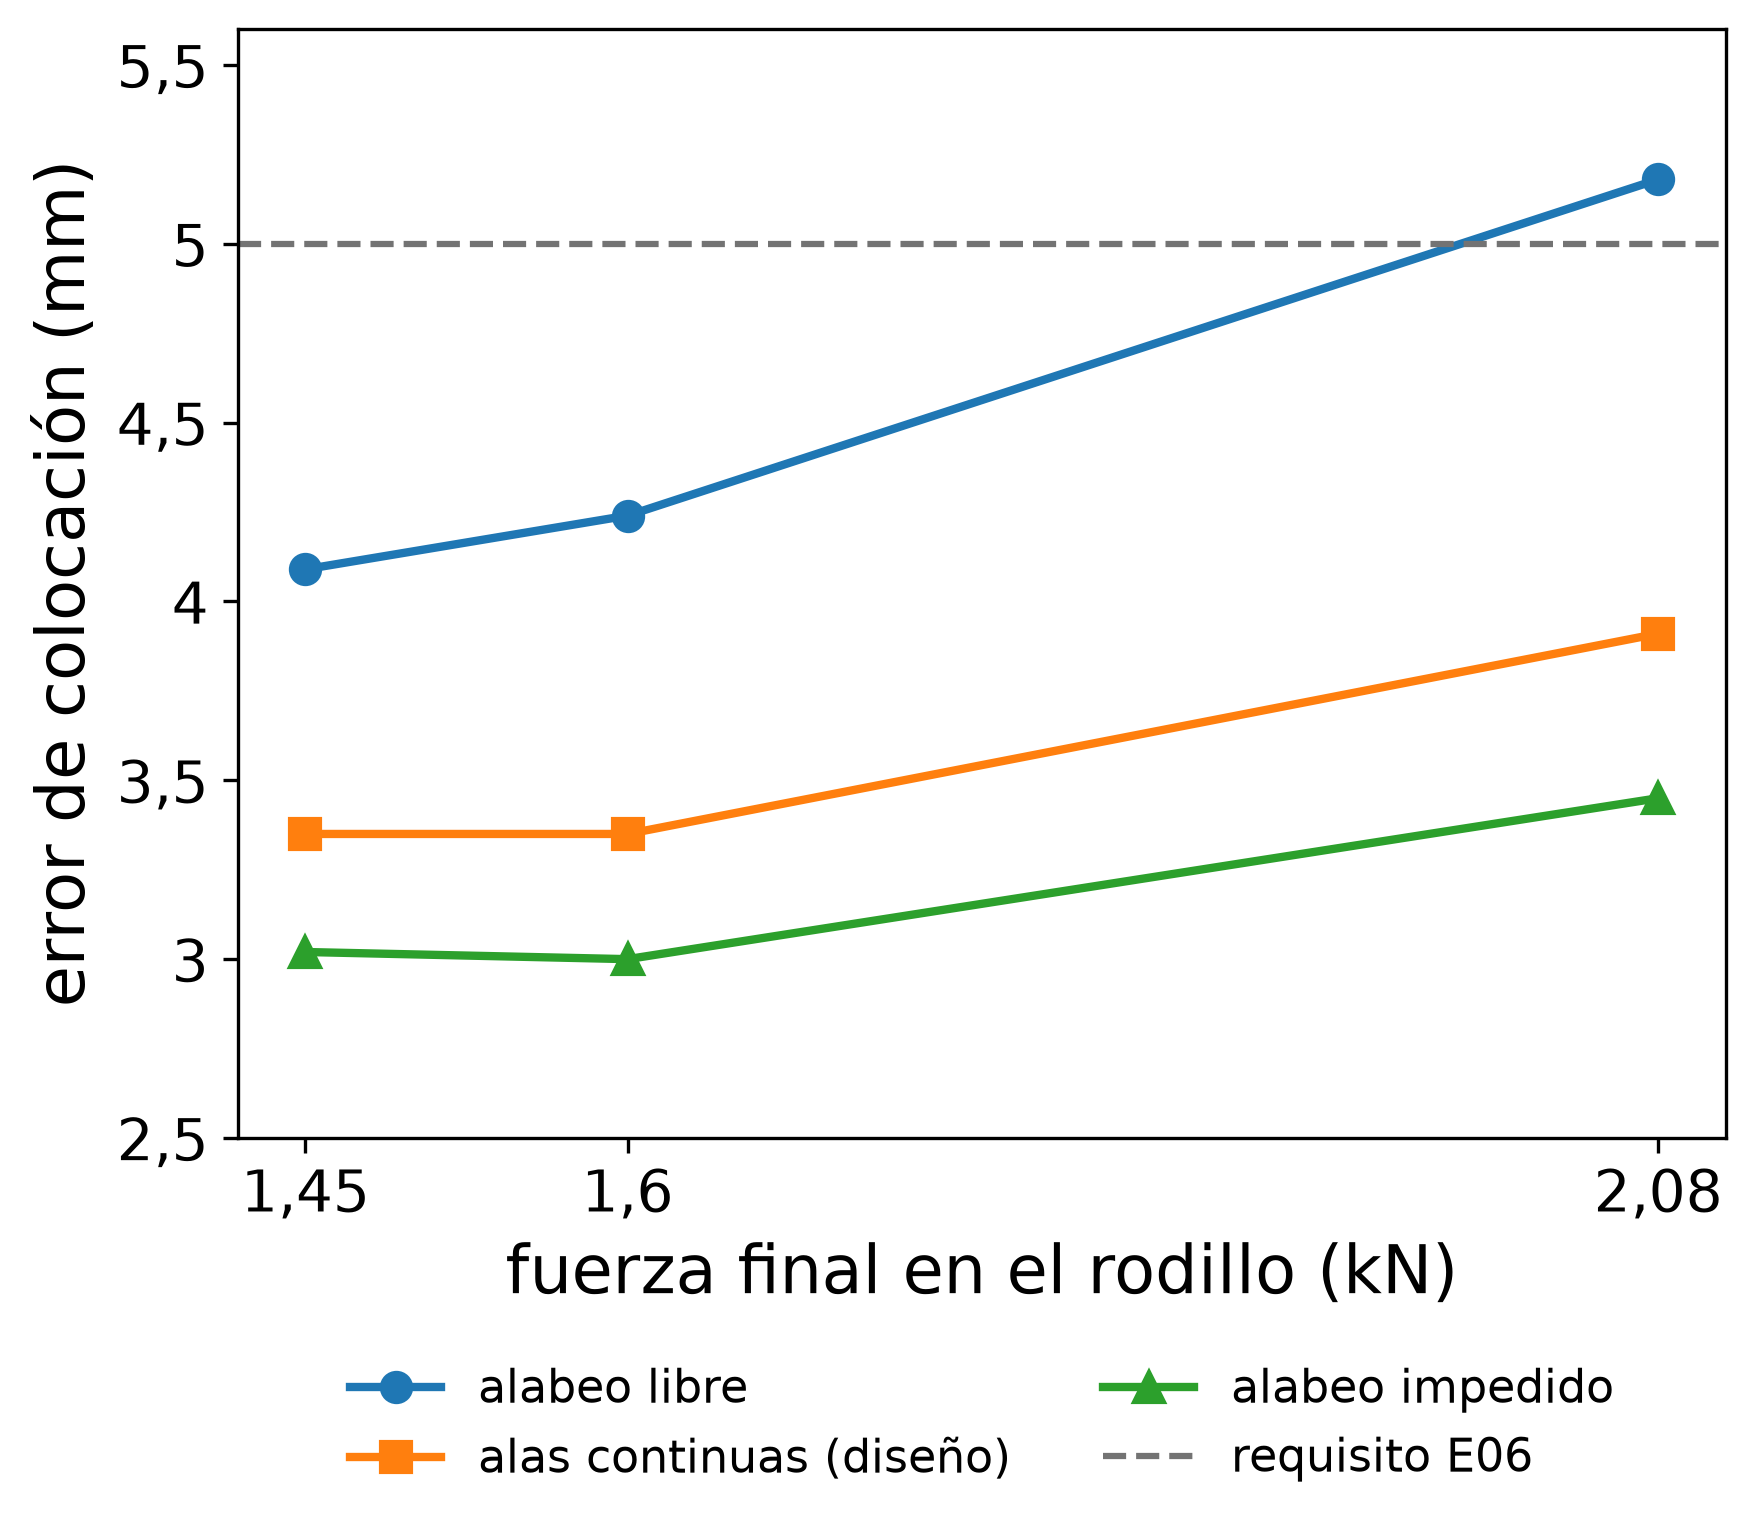
\includegraphics[width=0.62\textwidth]{fig_error_colocacion.png}
\caption{Error de colocación del rodamiento según la fuerza final en el rodillo del centrador empujador y la condición de alabeo en los nudos del bastidor. Elaboración propia con los resultados del modelo de barras.}
\label{fig:centrado}
\end{figure}

El ajuste H7/g6 \cite{iso286} se especificó en el pasador de bloqueo de 25 mm, en los pivotes de los brazos y en los pasadores de los rodillos; con él, todos los juegos suman 0,121 mm. A 2,08 kN, el 70\,\% del error es deformación elástica: 3,60 de 5,18 mm. Esa parte es lineal con la fuerza, con 1,731 mm/kN si el alabeo queda libre, y por eso el requisito se cumple mientras la fuerza final no pase de 1,97 kN. Se fijó entonces un requisito al limitador de fuerza del empujador: la fuerza final en el rodillo no debe pasar de 1,95 kN, incluida la dispersión del disparo. Con las alas continuas que da el detalle de uniones, el error baja a 3,35 mm en operación y a 3,91 mm en la envolvente.

Se evaluó y se descartó un cono de indexado en el pasador. Un cono solo elimina juego: llevaría el error de 5,18 a 5,14 mm, y aun sin ningún juego quedaría en 5,06 mm. Además, el pasador recibe hasta 1184 N en la estación de carga, un cono que no se autobloquea necesita otra pieza que lo mantenga asentado, y su asiento acumula grasa y agua alcalina. Apretar las tolerancias tampoco convenía: obligaría a mecanizar la mesa soldada para ganar apenas 0,05 mm.

\subsubsection{Bloqueo y retención}

La mesa se inmoviliza con el pasador central de 25 mm a doble corte, predimensionado para 10 kN, que se inserta en un receptor de la estación de carga antes de centrar y en otro de la estación de lavado antes de retraer los centradores. Tres topes bajos, a 60$^\circ$, 190$^\circ$ y 300$^\circ$, retienen el aro si este se desplaza sobre los apoyos; su unión al bastidor se detalla en los planos del Anexo~\ref{anx:planos}.

\subsection{Subsistema de aspersión}
\label{sec:dimensionamiento-aspersion}

\subsubsection{Caudal por boquilla y número de boquillas}

Con la Ecuación~\eqref{eq:teo-boquilla} y el punto de catálogo (7,571 L/min a 2,758 bar), el caudal de una boquilla a 4 bar resultó
\begin{equation}
q=q_r\sqrt{\frac{p_n}{p_r}}=7{,}571\sqrt{\frac{4{,}000}{2{,}758}}=9{,}118\ \mathrm{L/min},
\label{eq:dis-q-boquilla}
\end{equation}
con velocidad característica $v_j=C_v\sqrt{2p_n/\rho}=27{,}1$ m/s. Las boquillas de 15$^\circ$ tienen la misma capacidad nominal que las de 50$^\circ$, por lo que el mismo cálculo vale para ambas; solo cambia el abanico. El número de boquillas de cada grupo se obtuvo con la huella del abanico (Ecuación~\eqref{eq:teo-huella}) y la condición de solape:
\begin{equation}
N\geq1+\frac{L-b}{b(1-\phi)}.
\label{eq:dis-numero-boquillas}
\end{equation}
Para la lanza, con $L=515$ mm, distancia de 143,3 mm y $b=2(143{,}3)\tan25^\circ=133{,}6$ mm, resultó $N\geq4{,}81$; se adoptaron cinco boquillas, con un solape nominal de 28,7\,\%. Los grupos superior y exterior se dimensionaron del mismo modo. La Tabla~\ref{tab:boquillas-grupos} compara las tres configuraciones que se calcularon.

\begin{table}[htbp]
\centering\small\singlespacing
\caption{Distribución de boquillas del caso analítico, de la configuración base y de la configuración propuesta}
\label{tab:boquillas-grupos}
\begin{tabular}{@{}lccc@{}}
\toprule
\textbf{Grupo} & \textbf{Caso analítico} & \textbf{Base} & \textbf{Propuesta}\\
\midrule
Laterales exteriores ($2$ brazos) & $2\times5$ & $2\times5$ & $2\times5$\\
Superiores ($2$ brazos) & $2\times2$ & $2\times2$ & $2\times2$\\
Lanza interior (agujero) & 5 & 5 & 5\\
Inferior interior (lanza) & --- & 1 & 1\\
Inferiores exteriores (2 brazos) & --- & $2\times1$ & $2\times2$\\
\midrule
\textbf{Total simultáneo} & \textbf{19} & \textbf{22} & \textbf{24}\\
\bottomrule
\end{tabular}
\end{table}

\subsubsection{Configuración inferior}
\label{sec:configuracion-inferior}

La simulación de la configuración base mostró que la cara inferior recibía unas cuatro veces menos dosis que las demás superficies (Sección~\ref{sec:resultados-aspersion}). La causa era geométrica. La boquilla inferior exterior salía unos 35 a 40 mm bajo la cara, inclinada 30$^\circ$, y su eje llegaba al radio de 710 mm a una altura de unos 928 mm: mojaba la parte baja del diámetro exterior y no la cara inferior. Agregar caudal sin cambiar la geometría no resolvía la zona exterior de la cara.

Se compararon alternativas con trazado de rayos y se eligió un par de boquillas de abanico estrecho (15$^\circ$) en cada brazo. La boquilla inferior existente se reorientó a 15$^\circ$, de modo que llega a la cara en el radio de unos 687 mm, y se agregó otra a 10,7$^\circ$, que llega en el radio de unos 624 mm, separadas 60 mm. Las dos van en un bloque portaboquillas mecanizado de acero inoxidable. La red pasa de 22 a 24 boquillas: 20 de 50$^\circ$ y 4 de 15$^\circ$. Además, la primera boquilla lateral de cada brazo se inclinó 4$^\circ$ hacia abajo, con su punta fija, para cerrar una franja seca de 2 mm del diámetro exterior. El efecto de estos cambios en el mojado se evaluó con CFD y se analiza en la Sección~\ref{sec:resultados-aspersion}.

Para fijar las tolerancias de soldadura de las coplas, se perturbó cada boquilla con trazado de rayos en 240 casos de $\pm2$ mm y $\pm1^\circ$. Las coplas de 50$^\circ$ cambiaron la dosis como máximo un 2,8\,\%. Las salidas de 15$^\circ$ del bloque inferior, que llegan casi rasantes, perdían hasta un 18\,\%; por eso al bloque mecanizado se le asignaron $\pm0{,}5^\circ$ y $\pm1$ mm, con pérdidas de hasta 9,4\,\%. El criterio de 10\,\% es una hipótesis de los autores, y el trazado de rayos es un cribado del primer impacto, no un CFD.

\subsubsection{Red hidráulica, altura de bombeo y potencia}

La red se resolvió por aproximaciones sucesivas: con la Ecuación~\eqref{eq:teo-perdidas} y el factor de fricción de Swamee--Jain \cite{manSwamee}, se calcularon las pérdidas de cada tramo y se ajustó la presión de alimentación hasta que la boquilla más desfavorable recibiera 4 bar. La altura de bombeo se obtuvo con la Ecuación~\eqref{eq:teo-energia} entre la superficie libre del depósito y el cubo distribuidor, y la potencia con la Ecuación~\eqref{eq:teo-potencia}. El guion de cálculo reprodujo primero el caso analítico de diecinueve boquillas con las mismas cifras. La Tabla~\ref{tab:red-hidraulica} da los resultados de las tres configuraciones.

\begin{table}[htbp]
\centering\small\singlespacing
\caption{Resultados de la red hidráulica por configuración}
\label{tab:red-hidraulica}
\begin{tabularx}{\textwidth}{@{}Yccc@{}}
\toprule
\textbf{Magnitud} & \textbf{19 boquillas} & \textbf{22 boquillas} & \textbf{24 boquillas}\\
\midrule
Caudal total (L/min) & 173,99 & 202,59 & 221,07\\
Boquilla más desfavorable & Superior & Lanza & Lanza\\
Presión en las boquillas (bar) & 4,00--4,06 & 4,00--4,14 & 4,00--4,13\\
Altura de bombeo (m) & 50,75 & 52,56 & 53,39\\
Velocidad en DN40 (m/s) & 2,02 & 2,35 & 2,57\\
Potencia hidráulica (kW) & 1,42 & 1,71 & 1,90\\
Potencia al eje, $\eta_p=0{,}55$ (kW) & 2,58 & 3,11 & 3,45\\
\bottomrule
\end{tabularx}
\par\smallskip\footnotesize
Las tres columnas suponen una alimentación de 14 m en DN40. Con el trazado del modelo integrado, la altura de la red de 24 boquillas baja a 50,98--51,29 m.
\end{table}

Con 24 boquillas, el caudal sube un 9,1\,\% y la altura un 0,83 m respecto de la red de 22. La boquilla más alta de la lanza sigue fijando la presión del cubo en 4,063 bar, y las boquillas existentes cambian su presión en menos de 10 mbar, es decir, menos del 0,12\,\% en caudal. Por eso las superficies que no cambiaron de boquillas conservan los resultados de la simulación anterior.

Las alturas de la tabla suponen 14 m de alimentación en DN40 a 2,57 m/s. El modelo integrado tiene, en cambio, 8,7 m de tubería DN50 a 1,56 m/s hasta la unión rotativa; con ese trazado, la altura requerida es de 50,98 m con el tanque en su nivel normal y de 51,29 m en el nivel bajo. La subida hasta la unión rotativa no suma altura estática, porque se recupera al bajar hasta el cubo. Se informan las dos cifras: 53,39 m es la cota del cálculo de la red y 51,0--51,3 m, la del trazado modelado.

Se seleccionó una bomba multietapa vertical Grundfos CRN 15-3 de acero inoxidable 316, con motor de 4 kW \cite[pp.~50--51]{grundfoscr}. En la curva del catálogo entrega unos 56 m a 13,3 m$^3$/h, con unos 3,0 kW en el eje y un rendimiento cercano al 65\,\%; son lecturas gráficas, con una incertidumbre de $\pm1$ m en la altura. Le sobran de 2,6 a 4,7 m según la altura que se tome; ese exceso se recorta con un variador de frecuencia ajustado para que la boquilla más desfavorable reciba 4,00 bar. El NPSH disponible, con la presión atmosférica de 2335 m y la presión de vapor a 62~$^\circ$C, es de 5,24 a 5,55 m según el nivel del tanque \cite{white2016}, frente a unos 2,2 m requeridos por la bomba, valor conservador respecto de su curva. La potencia al eje de la Tabla~\ref{tab:red-hidraulica} usa un rendimiento supuesto de 0,55; con el de catálogo, la demanda es menor. La memoria de la red está en el Anexo~\ref{anx:calculos}.

\subsubsection{Distribuidor giratorio, eje y cubo}
\label{sec:distribuidor}

El distribuidor en U gira sobre un eje hueco, por cuyo interior pasa la alimentación hasta un cubo que reparte el caudal a la U y a la lanza (planos del eje, del cubo y de la U en el Anexo~\ref{anx:planos}). Para verificarlo se tomó la masa del modelo CAD, con 148 sólidos y el agua en los tubos. La estimación anterior era una envolvente de 180 kg con 50 mm de excentricidad; el modelo dio 231 kg con el centro de gravedad a 79,6 mm del eje, de modo que el momento excéntrico pasó de 88 a 180 N\,m. Como esa excentricidad gira con el eje, el peso produce una tensión constante en el eje; la única flexión alterna es la de la correa, que tira siempre en la misma dirección.

Las cargas fueron el peso y la excentricidad medidos, un par de 60 N\,m (el limitador desliza), un tiro de correa de 1071 N, la reacción de los chorros de 97 N, una carga accidental de 1000 N horizontal a 1400 mm del piso y una presión de 6 bar, con prueba hidrostática a 9 bar. Los 1071 N son una envolvente conservadora del tiro de la correa: el motorreductor se verificó con los 625 N que resultan del par limitado. La carga accidental y la presión son hipótesis de diseño. La Tabla~\ref{tab:conjunto-giratorio} reúne la verificación.

\begin{table}[htbp]
\centering\small\singlespacing
\caption{Verificación del distribuidor giratorio, su eje y su cubo}
\label{tab:conjunto-giratorio}
\begin{tabularx}{\textwidth}{@{}Yllr@{}}
\toprule
\textbf{Elemento y caso} & \textbf{Método} & \textbf{Resultado} & \textbf{D/C}\\
\midrule
Eje en el asiento del rodamiento inferior, accidental & von Mises & 37,4 MPa & 0,27\\
Eje en la polea, con chavetero, accidental & von Mises & 15,6 MPa & 0,11\\
Fatiga del eje en la polea & Goodman, Ec.~\eqref{eq:mt-goodman} & $\sigma_a=\sigma_m=4{,}9$ MPa & $n_f=24$\\
Flecha en las boquillas, servicio & Viga con voladizo & 0,36 mm y 0,31 mrad & --\\
Tubería junto al cubo, cargas sostenidas & ASME B31.3 \cite{asmeb313} & 13,4 MPa & 0,13\\
Codo de reducción, carga ocasional & ASME B31.3 & 100,5 MPa & 0,74\\
Tubería junto al cubo, carga ocasional tangencial & ASME B31.3 & 126,4 MPa & 0,93\\
Placas del cubo a 6 bar, borde empotrado & Placa circular & 60,6 MPa & 0,59\\
Placas del cubo en la prueba a 9 bar & Placa circular & 91 MPa & 0,66\\
Unión del eje con el cubo, filete de 5 mm & Cordón circular & 17,3 MPa & 0,05\\
\bottomrule
\end{tabularx}
\par\smallskip\footnotesize
Acero inoxidable 316L con $f_y=170$ MPa, reducido a 153 MPa a 62~$^\circ$C (hipótesis).
\end{table}

La resistencia no fija el tamaño del eje: lo fijan el paso de la alimentación por dentro y los asientos de 110 mm. La flecha de servicio en las boquillas es el 18\,\% de la tolerancia supuesta para el CFD. El único valor alto de la U, 0,93, corresponde a la carga accidental tangencial en un brazo, que solo puede ocurrir con el rotor detenido; con el rotor libre, el limitador desliza con 67 N en la punta del brazo. Las verificaciones complementarias con sólidos (Anexo~\ref{anx:calculos}) muestran que ese mismo golpe de 1000 N produce fluencia local en el tubo junto a la soldadura del transversal con el cubo, mientras la sección general trabaja al 74\,\% de la fluencia. Con el tramo central del transversal en DN50 Sch 80S, de igual diámetro exterior, la misma simulación deja la unión bajo la fluencia, con un margen de 1,23, sin cambiar las bridas ni el cordón; se recomienda esa variante. Las placas de 15 mm del cubo cumplen solo si se sueldan al anillo con penetración completa: el anillo es 15,5 veces más rígido al giro que la placa, lo que justifica tomar el borde como empotrado. Con borde apoyado, la prueba a 9 bar daría 1,09; por eso el requisito quedó escrito en el plano del eje y el cubo.

El cubo se suelda al eje y ambos se mecanizan en una sola atada, de modo que los asientos de los rodamientos y la cara inferior del cubo quedan alineados. La alternativa bridada con espiga H7/g6 sumaba una brida, seis pernos, una junta tórica expuesta al detergente a 62~$^\circ$C y unos 5 kg, sin una ventaja de resistencia: las dos uniones dan D/C $\leq0{,}06$. La U se desmonta por dos juntas bridadas DN50 a 300 mm del eje, sin válvulas de ramal, y sus dos brazos son iguales; en cada junta, el perno más cargado lleva 1,16 kN frente a 70,7 kN (D/C 0,02). Ninguna boquilla cambió de posición, de modo que el CFD sigue siendo válido para esta geometría.

El distribuidor gira con un motorreductor de 0,12 kW a través de una correa con relación 2:1. El limitador de par va en el eje de salida del motorreductor, ajustado a 30 N\,m, que equivalen a 60 N\,m en el rotor. Sin limitador, un atasco llevaría la carga radial de ese eje a 3,9 kN y no pasaría; con él, la carga radial es de 625 N según el método del fabricante y el factor de seguridad, de 2,31. El soporte superior que sostiene el conjunto y la selección del accionamiento se resumen en el Anexo~\ref{anx:calculos}.

\subsubsection{Cinemática del distribuidor}

A 1,7 rpm, una vuelta del distribuidor dura 35,3 s. La velocidad de barrido de las boquillas exteriores, a un radio de 836 mm, es de 0,149 m/s, y la de la lanza, 0,055 m/s. El tiempo de vuelo de las gotas hasta la superficie, de unos 7 ms a la mayor distancia, es pequeño frente al período de giro, lo que justifica evaluar la dosis con el distribuidor detenido por sectores (Sección~\ref{sec:teo-cfd}).

\subsubsection{Temperatura del baño}
\label{sec:calentamiento}

El detergente seleccionado no forma espuma por encima de 61~$^\circ$C y admite hasta 70~$^\circ$C \cite{zep36342}, por lo que el lavado se plantea con el baño a 60--62~$^\circ$C. Las lavadoras comerciales de aspersión calientan el tanque con resistencias de inmersión o con un quemador a gas, ofrecen un intercambiador de calor como opción y regulan la temperatura con un control electrónico: el StingRay 6075, con un depósito de 1325 L, usa 60 kW eléctricos o 117 kW a gas y tarda de 45 a 120 min en calentar el baño \cite{stingray_6075}. La máquina necesita un sistema equivalente. El esquema hidráulico lo representa con resistencias de inmersión y un control de temperatura en el tanque de lavado, como referencia de integración; su selección y su dimensionamiento quedan fuera del alcance.

\section{Selección de materiales, componentes y/o equipos de la solución}
\label{sec:seleccion-componentes}

Los componentes se seleccionaron a partir de los parámetros de las Secciones~\ref{sec:dimensionamiento-soporte} y~\ref{sec:dimensionamiento-aspersion}, con tres niveles: seleccionado, cuando el cálculo y el catálogo fijan una designación comercial; candidato, cuando la pieza es de fabricación propia y su geometría sale del modelo CAD y de los planos; y por confirmar, cuando falta un dato del fabricante. Los materiales en contacto con el agua alcalina a 62~$^\circ$C son de acero inoxidable 304 o 316. La Tabla~\ref{tab:seleccion-componentes} da el estado de cada componente, y el Anexo~\ref{anx:manuales} lista los catálogos y fichas empleados.

\begingroup
\footnotesize\singlespacing
\setlength{\parskip}{0pt}
\setlength{\tabcolsep}{4pt}
\renewcommand{\arraystretch}{1.05}
\begin{longtable}{@{}>{\raggedright\arraybackslash}p{2.7cm}>{\raggedright\arraybackslash}p{3.9cm}>{\raggedright\arraybackslash}p{\dimexpr\textwidth-2.7cm-3.9cm-2.2cm-6\tabcolsep\relax}>{\raggedright\arraybackslash}p{2.2cm}@{}}
\caption{Componentes de la solución y nivel de selección}\label{tab:seleccion-componentes}\\
\toprule
\textbf{Componente} & \textbf{Selección} & \textbf{Justificación} & \textbf{Estado}\\
\midrule\endfirsthead
\caption[]{Componentes de la solución y nivel de selección (continuación)}\\
\toprule
\textbf{Componente} & \textbf{Selección} & \textbf{Justificación} & \textbf{Estado}\\
\midrule\endhead
\midrule\multicolumn{4}{r}{\textit{Continúa en la página siguiente.}}\\\endfoot
\bottomrule\endlastfoot
\multicolumn{4}{@{}l}{\textit{Mesa y traslado}}\\
Bastidor & Perfil W6$\times$9, acero ASTM A36, uniones soldadas a momento & D/C máximo de 0,82 con el desvío lateral de las ruedas (Tabla~\ref{tab:uniones-bastidor}) & Candidato\\
Revestimiento de los apoyos & Polietileno de ultra alto peso molecular, 8 mm & Presión media de 0,85 MPa en servicio; protege la superficie del aro & Por confirmar\\
Rueda & Blickle SPKVS 200K, $\varnothing$200 mm, pestaña simple & D/C 0,89 en servicio y 0,43 frente a la capacidad estática \cite{blickle2026} & Seleccionada\\
Riel y pedestales & Riel A45 sobre 12 pedestales por riel de acero inoxidable 304 con 4 anclajes adhesivos M16 & Esfuerzos de 97,9 MPa con apoyos cada 580 mm o menos \cite{arcelor2023}; anclaje en el Anexo~\ref{anx:calculos} & Candidato\\
Traslado & Dos cadenas de rodillos 08B de acero inoxidable, eje de 25 mm, reductor sinfín de relación 5 y volante de 400 mm & Fuerza de 15,5 a 39,8 N en la empuñadura; parada con 190 N (Tabla~\ref{tab:traslado-verificacion}) & Candidato\\
Centradores & Brazo pivotante con dos referencias y un empujador de fuerza limitada a 1,95 kN & Selección multicriterio (Tabla~\ref{tab:seleccion-centradores}) y error de colocación (Tabla~\ref{tab:centrado-por-fuerza}) & Candidato\\
Bloqueo & Pasador $\varnothing$25 mm a doble corte con ajuste H7/g6 y receptores de carga y lavado & Retiene la mesa en el centrado y el lavado; error de colocación con juegos de 0,121 mm & Candidato\\
\multicolumn{4}{@{}l}{\textit{Aspersión e hidráulica}}\\
Boquillas & Spraying Systems VeeJet de acero inoxidable 316: 20 H3/8U-316SS5020 y 4 H3/8U-316SS1520 & Caudal de catálogo de 9,12 L/min a 4 bar en ambas; abanicos de 50$^\circ$ y 15$^\circ$ \cite{manSpray} & Seleccionadas\\
Distribuidor, eje y cubo & Tubo DN40 y DN50 Sch10S, eje hueco y cubo de 316L soldados y mecanizados & Verificación de la Tabla~\ref{tab:conjunto-giratorio} & Candidato\\
Tubería & DN15, DN25, DN40 y DN50 Sch10S de acero inoxidable 316L & ASME B36.19M \cite{asmeb3619}; 2,57 m/s en la alimentación DN40 del cálculo & Seleccionada para el cálculo\\
Fluido & Agua a 62~$^\circ$C con Zep Recirculating Detergent (7--15 g/L), alcalino de baja espuma & No forma espuma sobre 61~$^\circ$C y es compatible con acero y latón \cite{zep36342}; líquido acuoso \cite{en12921_2} & Seleccionado\\
Bomba & Grundfos CRN 15-3, multietapa vertical de 316, motor de 4 kW, con variador de frecuencia & Unos 56 m a 13,3 m$^3$/h frente a 51,0--53,4 m requeridos; NPSH requerido de unos 2,2 m frente a 5,2 m disponibles \cite{grundfoscr} & Seleccionada; lectura gráfica de la curva\\
Unión rotativa & Deublin 555-000-001, de un paso, con conexiones de 1-1/2 pulgadas NPT, carcasa de latón y rotor de acero inoxidable & Admite agua hasta 51,7 bar y 121~$^\circ$C \cite{deublin555}, frente a 6 bar de diseño, 9 bar de prueba y 62~$^\circ$C; su pérdida de 0,30 bar es supuesta & Seleccionada\\
Filtro & Filtro de bolsa Pentair ES2 de 316L, unos 150 µm & Filtración antes de las boquillas & Por confirmar la bolsa\\
Tanques & Lavado: 599 L de inoxidable 304, aislado, con 3 resistencias de 12 kW; enjuague: 204 L con inhibidor & Precalentamiento de unos 23 min (Sección~\ref{sec:calentamiento}) & Candidato\\
Drenaje & Colector de la cabina, línea por gravedad DN100 y pozo con bomba Hidrostal A02Q-S & Capacidad por gravedad de 413 L/min frente a 250 L/min (E14) & Candidato\\
\multicolumn{4}{@{}l}{\textit{Accionamiento y soporte del distribuidor}}\\
Motorreductor & SEW SF47R17DRN63MS4, 0,12 kW, con brida & Par de giro a 1,7 rpm con transmisión 2:1 & Seleccionado\\
Limitador de par & Mayr ROBA-slip tamaño 1, ajustado a 30 N\,m & Protege el eje de salida del motorreductor; factor de seguridad de 2,31 & Seleccionado\\
Soporte superior & Postes SHS80$\times$4 y vigas RHS150$\times$100$\times$3, 247 kg & Gobernado por rigidez; resumen en el Anexo~\ref{anx:calculos} & Candidato\\
\end{longtable}
\endgroup

El mecanismo de centrado se seleccionó con una matriz ponderada propia, precedida de diez condiciones excluyentes: ninguna pieza atraviesa los perfiles del bastidor ni entra bajo la huella del rodamiento, el contacto ocurre solo sobre la superficie autorizada del aro, los mecanismos son cautivos, tienen estados activo, retraído y de mantenimiento, se accionan con el distribuidor detenido, conservan el paso por la puerta y la holgura vertical de 18,8 mm, limitan la fuerza y superan los barridos del conjunto. Se compararon tres conceptos: un centrador de carro radial con poste, uno de brazo pivotante de eje vertical y uno de leva excéntrica (Tabla~\ref{tab:seleccion-centradores}).

\begin{table}[htbp]
\centering\small\singlespacing
\caption{Matriz ponderada de selección del mecanismo de centrado}
\label{tab:seleccion-centradores}
\begin{tabular}{lcccc}
\toprule
\textbf{Bloque de criterios} & \textbf{Peso} & \textbf{\makecell{Carro\\radial}} & \textbf{\makecell{Brazo\\pivotante}} & \textbf{Leva}\\
\midrule
Integración geométrica & 0,30 & 3,25 & 2,50 & 3,25\\
Mecánica y seguridad & 0,30 & 2,00 & 3,00 & 3,00\\
Fabricación y mantenimiento & 0,20 & 2,00 & 4,00 & 3,00\\
Entorno de lavado & 0,10 & 3 & 3 & 2\\
Efecto en masa y centro de gravedad & 0,10 & 4 & 5 & 4\\
\midrule
\textbf{Puntuación ponderada} & \textbf{1,00} & \textbf{2,675} & \textbf{3,250} & \textbf{3,075}\\
\bottomrule
\end{tabular}
\par\smallskip\footnotesize
Escala de 1 a 5. El centrador de carro radial no cumple la condición de tres estados por autointerferencia del poste retraído. Elaboración propia.
\end{table}

Se seleccionó el centrador de brazo pivotante. Su ventaja sobre el de leva fue de 0,175 puntos, y las tres evaluaciones por bloque no ordenaron igual a los conceptos. Se aceptó una menor nota de integración geométrica a cambio de un camino de cargas viable y de mejor fabricación y mantenimiento: el camino de cargas del centrador de leva quedó refutado y su carcasa fija, a 15 mm del diámetro exterior, sombreaba el lavado.

La bomba se eligió por el punto de la red y no por su potencia nominal. Se prefirió la versión de acero inoxidable 316 por el detergente alcalino, y el variador permite ajustar la presión de la boquilla más desfavorable a 4 bar sin estrangular la línea. El catálogo asigna a la CRN 15-3 un motor de 4 kW \cite{grundfoscr}; el presupuesto del Capítulo~\ref{cap:cronograma-presupuesto} la valoró por analogía con un motor de 3 kW, de modo que su precio debe confirmarse con la cotización. El revestimiento de los apoyos debe ser compatible con el fluido, la temperatura y la abrasión de las partículas retenidas; su resistencia declarada a compresión no sustituye la verificación de fluencia bajo carga sostenida. La rueda y el riel se verifican como sistema: la pestaña guía lateralmente y el juego de 3 mm entre pestaña y cabeza del riel debe compararse con la tolerancia de trocha de la instalación.

\section{Integración y/o implementación de los componentes en la solución final}
\label{sec:integracion}

La carga vertical sigue la ruta rodamiento $\rightarrow$ revestimiento y apoyos sectoriales $\rightarrow$ viga central y travesaños de carga $\rightarrow$ uniones soldadas a momento $\rightarrow$ vigas longitudinales $\rightarrow$ ruedas $\rightarrow$ rieles $\rightarrow$ pedestales anclados $\rightarrow$ losa. Los centradores y los topes transmiten acciones laterales por caminos distintos; el pasador de bloqueo retiene la mesa en el sentido del recorrido en las dos estaciones, y la cadena la controla entre ellas. El distribuidor y su accionamiento cargan sobre el soporte superior, que es independiente de la cabina y de la mesa.

\subsection*{Secuencia de operación}

La operación separa el izaje, el centrado, el traslado y la aspersión, de modo que nunca coinciden dos movimientos peligrosos:
\begin{enumerate}
\item con el distribuidor detenido a $0^\circ$, la lanza retirada y la red sin presión, la mesa vacía se lleva con el volante a la estación de carga, fuera de la cabina, y se inserta el pasador en el receptor de carga;
\item el rodamiento se iza y se apoya sobre los tres apoyos sectoriales;
\item con la grúa sosteniendo parcialmente el aro, los centradores lo llevan contra las dos referencias y el empujador se detiene al alcanzar su fuerza normal; se activan los topes y se retira el aparejo;
\item se retira el pasador, la mesa se lleva con el volante a la estación de lavado, se inserta el pasador en el receptor de lavado y se retraen los centradores;
\item con la puerta cerrada y sin personal en la cabina, se baja la lanza y se ejecuta el lavado con el baño a 60--62~$^\circ$C;
\item la válvula de succión cambia al tanque de enjuague, se enjuaga y se deja escurrir;
\item se despresuriza la red, el distribuidor se detiene a $0^\circ$, se retira la lanza y la mesa vuelve a la estación de carga para retirar el rodamiento.
\end{enumerate}

El distribuidor solo puede girar, y la lanza bajar, con la mesa bloqueada en la estación de lavado. El traslado exige el distribuidor detenido a $0^\circ$, porque en las posiciones de $30^\circ$, $60^\circ$ y $90^\circ$ los barridos presentaron contacto. Estas condiciones se trasladan a los enclavamientos del Capítulo~\ref{cap:seguridad-ambiente}.

\subsection*{Interfaces}

La integración geométrica se verificó con barridos del modelo CAD en traslado, giro del distribuidor, retirada de la lanza y accionamiento de los centradores. La holgura vertical que gobierna en el modelo anterior es de 18,8 mm, entre el ala superior del bastidor ($Z=805$ mm) y los pies de la U ($Z=823{,}8$ mm), sin tolerancias aplicadas; en el modelo integrado final, el barrido del traslado completo no encontró choques (Sección~\ref{sec:representacion}). La Tabla~\ref{tab:interfaces-criticas} reúne las interfaces que condicionan la integración.

\begingroup
\footnotesize\singlespacing
\setlength{\parskip}{0pt}
\setlength{\tabcolsep}{4pt}
\renewcommand{\arraystretch}{1.05}
\begin{longtable}{@{}>{\raggedright\arraybackslash}p{2.8cm}>{\raggedright\arraybackslash}p{\dimexpr(\textwidth-2.8cm-2.2cm-6\tabcolsep)/2\relax}>{\raggedright\arraybackslash}p{\dimexpr(\textwidth-2.8cm-2.2cm-6\tabcolsep)/2\relax}>{\raggedright\arraybackslash}p{2.2cm}@{}}
\caption{Interfaces críticas de integración}\label{tab:interfaces-criticas}\\
\toprule
\textbf{Interfaz} & \textbf{Condición documentada} & \textbf{Verificación en la etapa de detalle} & \textbf{Estado}\\
\midrule\endfirsthead
\caption[]{Interfaces críticas de integración (continuación)}\\
\toprule
\textbf{Interfaz} & \textbf{Condición documentada} & \textbf{Verificación en la etapa de detalle} & \textbf{Estado}\\
\midrule\endhead
\midrule\multicolumn{4}{r}{\textit{Continúa en la página siguiente.}}\\\endfoot
\bottomrule\endlastfoot
Rodamiento--apoyos & Huella completa con error radial de 5 mm & Presión local, revestimiento y orientación del cono & Parcial\\
Mesa--distribuidor & Holgura de 18,8 mm; barrido del traslado sin choques & Holgura con tolerancias y flechas & Verificado en CAD nominal\\
Centradores--distribuidor & Sombra de los centradores retraídos sobre el diámetro exterior: visibilidad de 99,81 a 99,71\,\% & Efecto sobre la configuración de 24 boquillas & Parcial\\
Soporte--CFD & Los obstáculos del CAD coinciden con el modelo de mojado; las cartelas de los topes bajan la dosis como máximo un 0,19\,\% & Contrastar con la geometría final & Verificado\\
Rueda--riel & D/C 0,89 en servicio y 0,43 en estado último; fuerza lateral de 6,51 kN & Capacidad a baja velocidad y juego de la pestaña & Fabricante\\
Riel--losa & Pedestales con 4 anclajes M16; levantamiento de 3,78 kN & Losa real y producto adhesivo & Dato de planta\\
Distribuidor--soporte superior & Desplazamiento lateral del cojinete de 2,26 mm frente a 22,9 mm de holgura en el techo & Velocidad del motor frente a los modos del soporte & Verificado por simulación\\
Mesa--puerta & Recorrido de 3320 mm y paso por la puerta modelada & Levantamiento de planta y aparejo de grúa & Dato de planta\\
Bloqueo--control & Receptores de carga y lavado conectados al bastidor & Lógica de enclavamiento (Capítulo~\ref{cap:seguridad-ambiente}) & Definida en diseño\\
\end{longtable}
\endgroup

\subsection*{Circuito hidráulico}

El circuito se representó en un esquema de tuberías e instrumentación simplificado según ISO 10628-2, con 42 componentes e instrumentos (Figura~\ref{fig:esquema-hidraulico}). El agua del tanque de lavado pasa por la válvula de tres vías de succión, el colador y la bomba; sigue por la válvula de retención, la válvula de impulsión y el filtro de bolsa, sube por el montante hasta la unión rotativa y baja por el eje hueco hasta el cubo. Del cubo sale hacia la U, con 18 boquillas y sin válvulas de ramal, y hacia la lanza, con 6 boquillas, a través de una válvula de aislamiento y una manguera que sigue la carrera de 640 mm. El agua cae a la cabina y vuelve al tanque de lavado por el drenaje; para el enjuague, la válvula de succión cambia al tanque de 204 L. El esquema también representa el calentamiento del tanque, la dosificación del detergente y del inhibidor, el pozo de drenaje y un contenedor para la purga, como referencia de integración: esos elementos quedan fuera del alcance y no se dimensionaron. La hoja 2 del plano (Anexo~\ref{anx:planos}) señala para la etapa de detalle el tarado de la válvula de alivio, que comparte derivador con el caudal mínimo de la bomba, y la bolsa del filtro.

\begin{figure}[p]
\centering
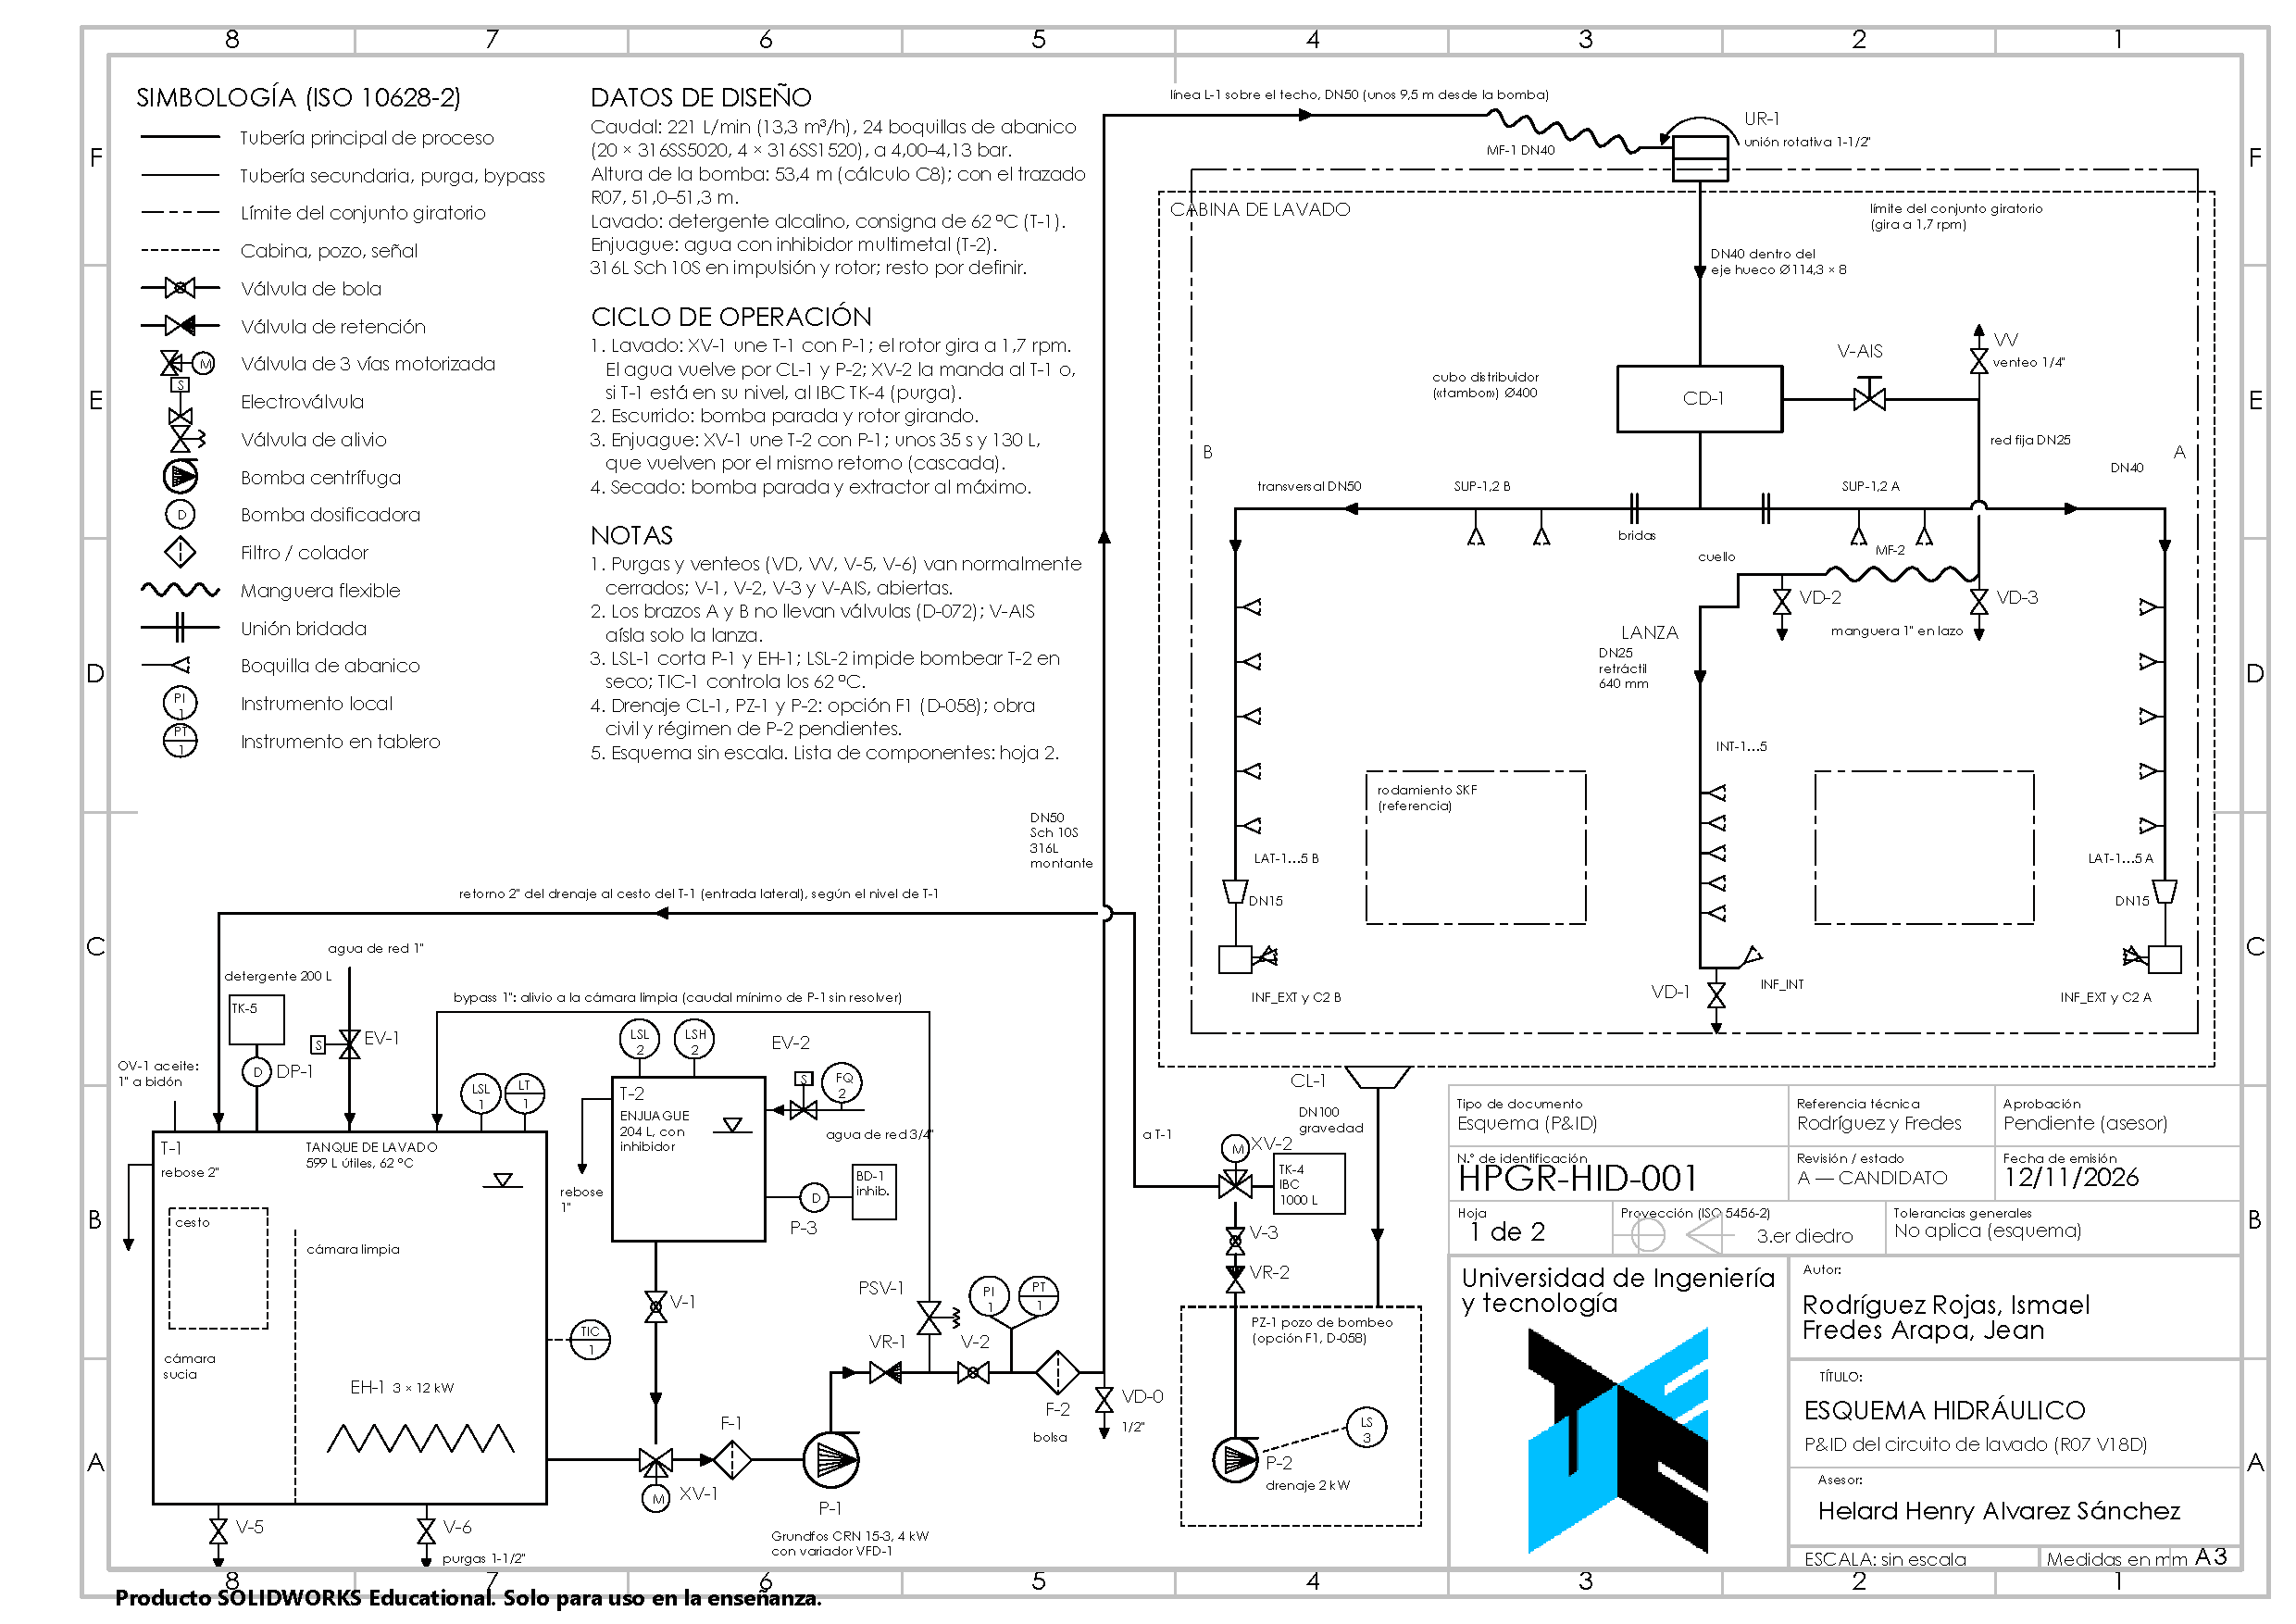
\includegraphics[angle=90,width=\textwidth,height=0.88\textheight,keepaspectratio]{HPGR-HID-001_hoja1.pdf}
\caption{Esquema hidráulico de la máquina, hoja 1: circuito, simbología, datos de diseño y ciclo. La hoja 2, con la lista de componentes, y el plano a tamaño completo están en el Anexo~\ref{anx:planos}. Elaboración propia en SolidWorks.}
\label{fig:esquema-hidraulico}
\end{figure}

\section{Representación gráfica de la solución y su verificación}
\label{sec:representacion}

La solución se representa con un modelo CAD integrado en FreeCAD y con planos normalizados emitidos en SolidWorks. El modelo reúne la mesa con sus centradores, el traslado, los rieles y pedestales, el sistema de aspersión, el soporte superior, la cabina, los tanques, la bomba, el tablero y el drenaje. Los componentes comerciales se representan con los modelos de sus fabricantes cuando estuvieron disponibles. La Figura~\ref{fig:cad-maquina} muestra el conjunto.

\begin{figure}[htbp]
\centering
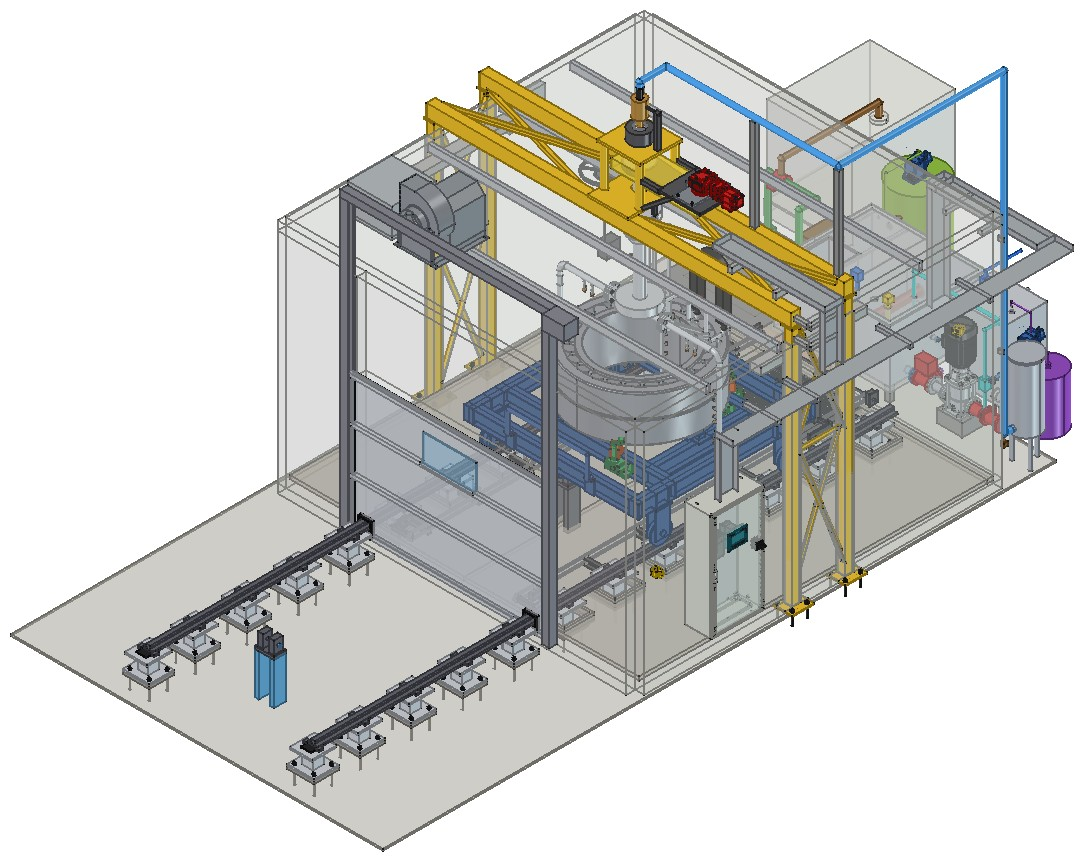
\includegraphics[width=0.70\textwidth]{cad_maquina_iso.jpg}
\caption{Modelo integrado de la máquina con la cabina transparente: mesa sobre rieles y pedestales, soporte superior con el motorreductor, distribuidor en U, tanques, bomba, tablero y puerta. Elaboración propia en FreeCAD.}
\label{fig:cad-maquina}
\end{figure}

\subsection*{Planos}

Se emitieron 34 planos con cotas, ajustes, tolerancias, lista de piezas y rótulo, más el esquema hidráulico de dos hojas (Tabla~\ref{tab:planos}). Se usó el sistema ISO con proyección en tercer diedro. Las soldaduras llevan símbolos ISO 2553 \cite{iso2553}, y las tolerancias generales son ISO 13920 clase B en los conjuntos soldados e ISO 2768-mK en las piezas mecanizadas. El Anexo~\ref{anx:planos} reúne los planos de conjunto y de los subconjuntos principales.

\begin{table}[htbp]
\centering\small\singlespacing
\caption{Planos emitidos}
\label{tab:planos}
\begin{tabularx}{\textwidth}{@{}lrY@{}}
\toprule
\textbf{Grupo} & \textbf{Cant.} & \textbf{Contenido}\\
\midrule
Mesa & 8 & Conjunto, bastidor con soldaduras, apoyo sectorial, rueda, topes (2), manillar y bloqueo central\\
Traslado y riel & 2 & Doble cadena con volante y pedestal del riel\\
Centradores & 16 & Dos de referencia y el empujador, con soporte y despiece\\
Aspersión & 6 & Sistema, eje y cubo, U, brazo, lanza y red\\
Soporte superior & 2 & Conjunto, base del poste y nudo viga--poste\\
Esquema hidráulico & 1 & Circuito y lista de componentes, en dos hojas\\
\midrule
\textbf{Total} & \textbf{35} & \\
\bottomrule
\end{tabularx}
\end{table}

\subsection*{Verificación del modelo}

Sobre el modelo final se hicieron tres revisiones independientes. La primera fue una auditoría geométrica en FreeCAD, que clasificó 146 solapes: todos son uniones representadas por solape u holguras internas ya declaradas, y ninguno es un choque nuevo. La segunda fue un barrido del traslado de 3320 mm cada 40 mm, con 292 piezas móviles frente a 323 fijas; marcó tres pares, dos del pasador de bloqueo dibujado insertado y uno de un objeto que agrupa bujes fijos y móviles, y ninguno es un choque real. La tercera fue la detección de interferencias en SolidWorks, como segunda opinión con otra herramienta. Marcó 79 interferencias en el conjunto de la mesa, 13 en el centrador empujador, 5 en el soporte de su pivote y 1 en el tope de 190$^\circ$; todas son uniones representadas por solape, ya declaradas. Los topes de 60$^\circ$ y 300$^\circ$, el traslado y el pedestal no tuvieron ninguna.

Las interferencias que quedan son representaciones del modelo y no choques, pero siguen dibujadas así. SolidWorks revisó cada ensamble por separado; las interacciones entre subsistemas las cubren la auditoría y el barrido. El barrido revisa sólidos cada 40 mm, no simula la cadena en movimiento y toma la U estacionada a 0$^\circ$. Los planos no están liberados para fabricación: faltan los planos de pieza de las barras, que hoy figuran en la lista de corte, y los de la cabina y el bloque portaboquillas. La evolución de la geometría desde la mesa circular hasta la configuración actual se registra en el Anexo~\ref{anx:iteraciones}.



\chapter{PRUEBAS Y RESULTADOS}
\label{cap:resultados}

\section{Plan de pruebas de la solución}
\label{sec:plan-pruebas}

La verificación se planificó por subsistema y por nivel de evidencia. Las pruebas son numéricas, analíticas y geométricas: análisis estructural del bastidor y de sus uniones, modelos de elementos finitos de los centradores, barridos en el modelo CAD, cálculo de la red hidráulica y simulación del mojado del rodamiento. Los ensayos físicos quedan fuera del alcance de la tesis; ningún resultado de este capítulo es una validación experimental.

Se adoptó un Caso Base por subsistema. Para el soporte, el Caso Base es el bastidor de tres apoyos sectoriales con el rodamiento centrado y una carga vertical de $3\times9948$ N. Para la aspersión, el Caso Base hidráulico fue la red de diecinueve boquillas y el Caso Base de mojado, la configuración de 22 boquillas a 1,7 rpm. A partir de ellos se plantearon escenarios de sensibilidad y de rediseño: combinaciones de carga con factores 1,00, 1,25 y 1,40; fuerza final del centrador de 1,45 a 2,08 kN; desvío lateral de una rueda; presión uniforme de 3 a 6 bar en las boquillas; cambio de malla, paso de tiempo, dominio y número de parcelas del modelo de mojado; y las variantes de boquillas del diámetro exterior y de la cara inferior. La Tabla~\ref{tab:plan-pruebas} asigna a cada prueba sus escenarios, sus variables, su criterio y su estado.

\begingroup
\small\singlespacing
\setlength{\tabcolsep}{3.5pt}
\renewcommand{\arraystretch}{1.08}
\begin{longtable}{@{}>{\raggedright\arraybackslash}p{2.9cm}>{\raggedright\arraybackslash}p{3.7cm}>{\raggedright\arraybackslash}p{3.0cm}>{\raggedright\arraybackslash}p{1.9cm}>{\raggedright\arraybackslash}p{\dimexpr\textwidth-11.5cm-10\tabcolsep\relax}@{}}
\caption{Plan de pruebas, escenarios y estado}\label{tab:plan-pruebas}\\
\toprule
\textbf{Prueba} & \textbf{Caso Base y escenarios} & \textbf{Variables medidas} & \textbf{Criterio} & \textbf{Estado}\\
\midrule\endfirsthead
\caption[]{Plan de pruebas, escenarios y estado (continuación)}\\
\toprule
\textbf{Prueba} & \textbf{Caso Base y escenarios} & \textbf{Variables medidas} & \textbf{Criterio} & \textbf{Estado}\\
\midrule\endhead
\midrule\multicolumn{5}{r}{\textit{Continúa en la página siguiente.}}\\\endfoot
\bottomrule\endlastfoot
Análisis estructural del bastidor & Carga centrada; factores 1,00, 1,25 y 1,40; desvío lateral de una rueda y tiro de las cadenas & Reacciones, flecha relativa, D/C de barras y uniones & E03, E04, E05 & Ejecutada\\
Modelo global con cargas de centrado & 1,45, 1,60 y 2,08 kN; alabeo libre, continuo o impedido en los nudos & Desplazamiento en el contacto del centrador & E06, E08 & Ejecutada\\
Elementos finitos locales de los centradores & 2,08 kN; dos mallas y dos sentidos de carga & Desplazamiento radial y tensiones & E06, E08 & Ejecutada\\
Error de colocación y captura & Fuerza final del empujador; excentricidad de 5 mm en ocho direcciones & Error de colocación y carrera de captura & E06, E08 & Ejecutada (cálculo)\\
Barridos CAD e interferencias & Traslado, giro del distribuidor, retirada de la lanza y centradores & Holgura mínima y contactos & E01, E07, E15 & Ejecutada\\
Red hidráulica & 19, 22 y 24 boquillas; presión uniforme de 3 a 6 bar & Presión por boquilla, caudal, altura, potencia, NPSH & E09--E11 & Ejecutada\\
Simulación del mojado & 22 boquillas a 1,7 rpm; malla, $\Delta t$, dominio y parcelas; caso puente & Acceso, dosis, uniformidad, zona seca, transferencia e impulso & E12, E13 & Ejecutada\\
Rediseño de boquillas & Lateral inclinada y superior desplazada; par inferior de abanico estrecho (24 boquillas) & Dosis, uniformidad, zona seca y transferencia & Regla de decisión; criterio de la zona exterior & Ejecutada\\
Alcance del lavado & Dosis requerida de 65, 183 y 305 kg\,m$^{-2}$; trazado de rayos del rodamiento armado & Tiempo hasta la dosis requerida; área visible de rodillos y pistas & E13 & Ejecutada (cálculo)\\
\end{longtable}
\endgroup

El mojado se evalúa con seis indicadores propuestos por el equipo (Tabla~\ref{tab:kpi-cfd}). Miden si el líquido llega a cada superficie, cuánto llega, con qué uniformidad y con qué cantidad de movimiento; no miden la remoción de grasa, que solo puede establecerse con ensayo.

\begin{table}[htbp]
\centering\small\singlespacing
\caption{Indicadores del modelo de mojado}
\label{tab:kpi-cfd}
\begin{tabularx}{\textwidth}{@{}lY@{}}
\toprule
\textbf{Indicador} & \textbf{Definición}\\
\midrule
Acceso geométrico & Fracción del área mojable que alcanzan los chorros, por trazado de rayos con los obstáculos del soporte\\
Dosis de mojado & Masa depositada por unidad de área y por vuelta del distribuidor, $D$, media y mínima por bandas (Sección~\ref{sec:teo-cfd})\\
Uniformidad & Coeficiente de variación de $D$ entre bandas de 10 mm (y de 2 mm, complementario)\\
Zona seca & Fracción de bandas sin impacto directo, y área con $D\geq5$ kg\,m$^{-2}$ por vuelta\\
Transferencia & Fracción del caudal de las boquillas asignadas a una superficie que llega a ella, $\eta$\\
Acción hidráulica & Impulso por unidad de área y por vuelta, $J$, y presión media de huella\\
\bottomrule
\end{tabularx}
\end{table}

\section{Análisis de los resultados de las pruebas}

\subsection{Subsistema de soporte}
\label{sec:resultados-soporte}

\subsubsection{Caso Base: análisis estructural del bastidor}

El bastidor de tres apoyos sectoriales se analizó en SAP2000 como pórtico de barras W6$\times$9 de acero ASTM A36, con las cargas del rodamiento en los nodos de los apoyos sectoriales y cuatro apoyos en las posiciones de las ruedas \cite{csi_analisis_2016}. Los apoyos son bilaterales: el nodo 2 restringe los tres desplazamientos y los nodos 5, 13 y 16 restringen los desplazamientos en $X$ y $Z$; las rotaciones quedan libres. La Figura~\ref{fig:modelo-r01} muestra el modelo y la Tabla~\ref{tab:combinaciones-r01}, las combinaciones.

\begin{figure}[htbp]
\centering
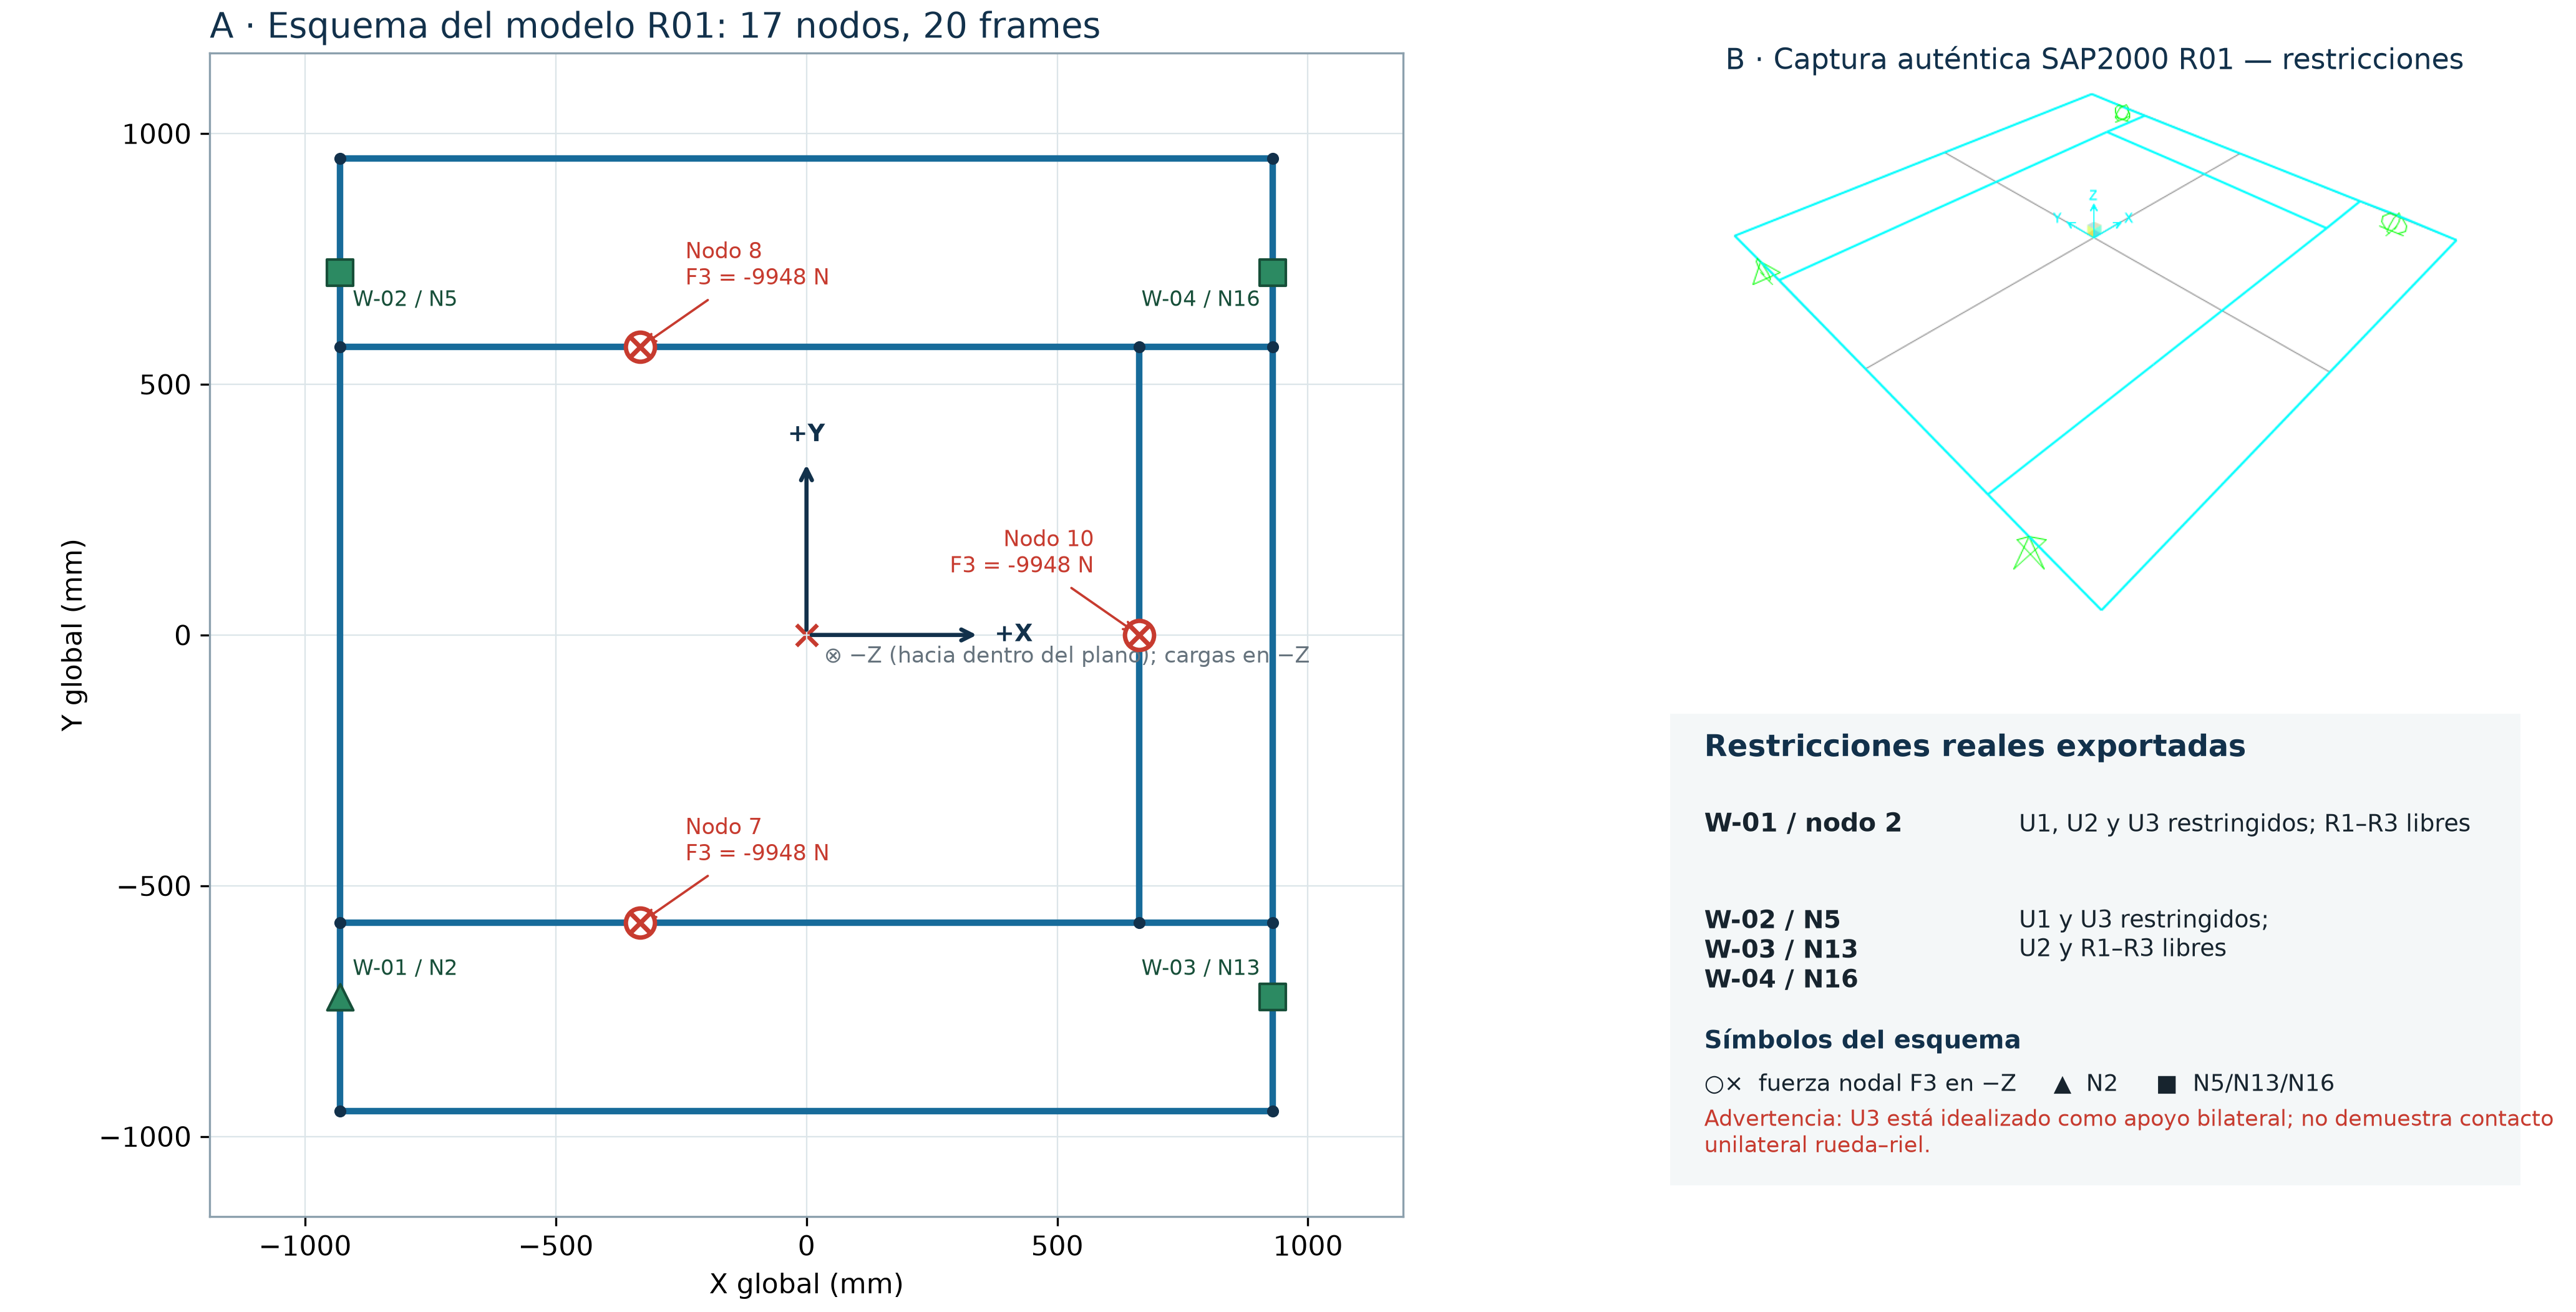
\includegraphics[width=0.84\textwidth]{images/sap/02_MODELO_CARGAS_APOYOS_R01_recorte.png}
\caption{Modelo estructural del bastidor de tres apoyos sectoriales: esquema de nodos, cargas y apoyos (izquierda) y restricciones en SAP2000 (derecha). Los apoyos verticales son bilaterales y no representan el contacto unilateral rueda--riel. Fuente: corrida del modelo en SAP2000 y posproceso propio.}
\label{fig:modelo-r01}
\end{figure}

\begin{table}[htbp]
\centering\small\singlespacing
\caption{Combinaciones de carga del análisis estructural}
\label{tab:combinaciones-r01}
\begin{tabularx}{\textwidth}{YP{3.2cm}P{3.6cm}}
\toprule
\textbf{Combinación} & \textbf{Peso propio del bastidor} & \textbf{Carga vertical en los apoyos} \\
\midrule
Nominal de servicio & 1,00 & 1,00 \\
Servicio con carga externa amplificada & 1,00 & 1,25 \\
Resistente & 1,40 & 1,40 \\
\bottomrule
\end{tabularx}
\end{table}

La combinación nominal sumó 29,844 kN de carga externa y 1,649 kN de peso propio, con una reacción total de 31,493 kN (Tabla~\ref{tab:reacciones-r01}). El cálculo manual del Anexo~\ref{anx:calculos} reprodujo las reacciones con diferencias no mayores que 0,004 N, lo que comprueba el equilibrio y el reparto del caso centrado. En la combinación resistente, la reacción total exportada fue de 44,090 kN, igual a $1{,}4(29{,}844+1{,}649)$ kN dentro de la precisión tabulada.

\begin{table}[htbp]
\centering\small\singlespacing
\caption{Reacciones verticales y resultados de servicio del bastidor}
\label{tab:reacciones-r01}
\begin{tabularx}{\textwidth}{@{}Yrr@{}}
\toprule
\textbf{Magnitud} & \textbf{Nominal de servicio} & \textbf{Carga externa $\times1{,}25$} \\
\midrule
Reacción en los nodos 2 y 5 / 13 y 16 (kN) & 7,846 / 7,900 & -- \\
Reacción individual máxima (kN) & 7,900 & 9,766 \\
Suma de reacciones verticales (kN) & 31,493 & 38,954 \\
Máximo nodal $|U_3|$ (mm) & 1,353 & 1,686 \\
Flecha relativa en el nodo del apoyo (mm) & 1,236 & 1,540 \\
Diferencia vertical entre apoyos (mm) & 0,294 & 0,367 \\
\bottomrule
\end{tabularx}
\end{table}
\label{tab:resultados-servicio}

El máximo nodal $|U_3|$ no es la flecha del miembro: para el travesaño de carga se evaluó el nodo del apoyo respecto de la cuerda de sus extremos con la Ecuación~\eqref{eq:mt-flecha}. Con la longitud del travesaño de 1860 mm, la flecha relativa nominal de 1,236 mm queda por debajo de $L/360=5{,}17$ mm, $L/800=2{,}33$ mm y $L/1000=1{,}86$ mm. Es una evaluación nodal; falta buscar el máximo continuo entre estaciones. La verificación de miembros con AISC 360-16 dio una razón demanda/capacidad máxima de 0,277 en los travesaños de carga, con la combinación resistente (Anexo~\ref{anx:programas}). Se compararon también bastidores de cuatro y cinco apoyos; el de tres tuvo la menor masa, 168,1 kg, con una flecha dentro de los límites, y se mantuvo (Anexo~\ref{anx:iteraciones}).

Ese modelo solo tenía cargas verticales. Al agregar el desvío lateral de una rueda durante el traslado, con 6,51 kN en el contacto, las vigas longitudinales pasaron de 0,28 a 0,82, y a 0,89 con el alabeo libre en los nudos (Tabla~\ref{tab:uniones-bastidor}). Las diez uniones a momento quedaron en D/C $\leq0{,}58$. El bastidor cumple, pero el margen que daba el caso vertical era engañoso: lo gobierna una carga del traslado que el primer modelo no tenía.

\subsubsection{Verificación global con las cargas de centrado}

Las cargas de los centradores son horizontales y excéntricas respecto del alma, de modo que torsionan los travesaños de carga. Con la torsión uniforme de Saint-Venant que emplea SAP2000 en sus barras, el desplazamiento en el contacto de una referencia resultó de 13 a 17 mm, un valor sin sentido físico porque ignora la rigidez al alabeo de la sección. Por ello se construyó un modelo global con siete grados de libertad por nudo, que incluye la torsión no uniforme \cite{aiscdg9}. Antes se replicó el pórtico en CalculiX: dos voladizos de calibración coincidieron con la solución analítica dentro del 2\,\% y el equilibrio cerró con residuos inferiores a $10^{-7}$ N.

Sumando la parte global y la local, el desplazamiento total en el contacto de la referencia resultó de 1,51 a 1,64 mm con uniones rígidas. Si los encuentros de los travesaños se resolvieran solo por el alma, subiría a 2,1--7,1 mm. Un travesaño adicional lo reducía a 0,77--0,78 mm, pero quedaba a 5,3--7,7 mm bajo el pie giratorio de la lanza y se retiró. El resultado llevó a diseñar las uniones a momento con continuidad de alas (Sección~\ref{sec:uniones-bastidor}) y a juzgar la deformación por su efecto sobre la colocación del rodamiento.

\subsubsection{Centradores y precisión del centrado}

Las referencias, con 0,48 a 0,59 mm en el contacto, cumplen el criterio local de 1,0 mm, aunque no siempre el objetivo de 0,5 mm. En el empujador, la placa de 20 mm del soporte del pivote presentó de 190 a 246 MPa de membrana más flexión, por encima del filtro de 150 MPa. Con una placa de 28 mm, la tensión bajó a 102--129 MPa y el desplazamiento de 1,58--1,65 a 0,89--0,91 mm; esa placa se adoptó, con soldaduras a tope de penetración completa.

En el modelo CAD, con el aro desplazado 5 mm en ocho direcciones, el rodillo de cada centrador tocó siempre antes que la horquilla, el pasador o el brazo, y la carrera de captura en el peor caso fue de 13,1 mm, frente a 5 mm de E08. La precisión era el punto débil de la segunda entrega: 5,21 mm en el caso nominal y 6,10 mm en la envolvente de 2,08 kN. Al separar la parte elástica de las tolerancias (Sección~\ref{sec:error-colocacion}), se vio que el 70\,\% del error a 2,08 kN es deformación y que crece con la fuerza. Con el ajuste H7/g6 y el límite de 1,95 kN al empujador, el error queda en 4,09 mm en la detención y 4,24 mm en el disparo, con alabeo libre, y en 3,35 mm con las alas continuas del detalle de uniones. La envolvente de 2,08 kN, que exige fallar la detención y el disparo, da 5,18 mm con alabeo libre y 3,91 mm con alas continuas.

\subsection{Subsistema de aspersión}
\label{sec:resultados-aspersion}

\subsubsection{Red hidráulica}

Al pasar de diecinueve a veintidós boquillas, el caudal aumentó un 16,4\,\% y la altura de bombeo un 3,6\,\%, y la boquilla más desfavorable pasó de una superior a la más alta de la lanza. Con 24 boquillas, el caudal subió otro 9,1\,\% y la altura 0,83 m (Tabla~\ref{tab:red-hidraulica}). Las presiones de las boquillas quedaron entre 4,00 y 4,13 bar, de modo que la red entrega un caudal casi uniforme. Entre 3 y 6 bar de presión uniforme, el caudal de la red de 22 boquillas pasa de 173,7 a 245,7 L/min y la escala de fuerza del chorro se duplica (Anexo~\ref{anx:calculos}). Más presión eleva la acción del chorro a costa de caudal y de energía, y su efecto sobre la limpieza solo puede comprobarse con ensayo.

\subsubsection{Modelo de mojado y verificación numérica}

El mojado se simuló en ANSYS Fluent con fase discreta lagrangiana acoplada en dos vías, aire con turbulencia $k$--$\varepsilon$ y paredes que retienen la gota en el primer impacto \cite{fluent2026}. El distribuidor se representó detenido en sectores de $\pm12^\circ$ alrededor de cada boquilla y la dosis por vuelta se obtuvo integrando la huella sobre la circunferencia (Sección~\ref{sec:teo-cfd}). Los obstáculos del soporte se aplicaron como máscaras de sombra por trazado de rayos. Una corrida con un apoyo sectorial incluido en la malla respaldó el método: a ese apoyo llegó el 16,9\,\% del caudal de la boquilla inferior exterior, frente al 18,0\,\% estimado con las máscaras. La configuración completa se detalla en el Anexo~\ref{anx:programas}.

La verificación de la configuración base comparó tres niveles de malla por dominio, con razones de refinamiento de 1,25 a 1,30, y estimó la incertidumbre de discretización con el índice de convergencia de malla \cite{celik2008}. Los cambios entre las dos mallas más finas y los de los demás estudios están en la Tabla~\ref{tab:verificacion-cfd} del Anexo~\ref{anx:programas}.

Los indicadores integrales cambiaron menos que el 5\,\% fijado como criterio de trabajo, y la mayoría menos del 1\,\%. En la cara inferior, los cambios quedaron dentro del ruido entre corridas equivalentes de los dos brazos ($\pm1{,}5$\,\% en $\bar D$), por lo que el índice de convergencia no es interpretable allí. La dosis mínima varió hasta $\pm18$\,\%, porque la fija una sola banda; se informa, pero no se usa para juzgar la convergencia. Con menos parcelas por boquilla aparecían zonas secas artificiales, lo que justificó usar 600 trayectorias por plano en las boquillas de incidencia normal y 1200 en las inferiores. El caso del agujero repetido en Fluent difirió del resuelto en OpenFOAM un 0,27\,\% en la dosis media; esa concordancia entre programas no equivale a una validación física.

\subsubsection{Resultados de la configuración base}

La Tabla~\ref{tab:cfd-caso-base} reúne los indicadores de la configuración base, con los obstáculos del soporte, y la Figura~\ref{fig:cfd-trayectorias} muestra las trayectorias de las gotas en el diámetro exterior y la cara inferior.

\begin{table}[htbp]
\centering\small\singlespacing
\setlength{\tabcolsep}{4pt}
\caption{Indicadores de la configuración base de 22 boquillas por superficie}
\label{tab:cfd-caso-base}
\begin{tabular}{lcccccc}
\toprule
\textbf{Superficie} & \textbf{\makecell{Acceso\\(\%)}} & \textbf{$\bar D$; $D_{mín}$} & \textbf{CV} & \textbf{Seca 10/2 mm (\%)} & \textbf{$\eta$ (\%)} & \textbf{$\bar J$}\\
\midrule
Diámetro exterior & 100 & 26,40; 0,44 & 0,302 & 0 / 0,39 & 94,3 & 609\\
Cara superior & 100 & 22,53; 6,13 & 0,396 & 0 / 0 & 97,9 & 527\\
Cara inferior & 100 & 5,46; 2,93 & 0,616 & 0 / 0 & 31,0 & 43\\
Agujero & 100 & 18,72; 11,52 & 0,339 & 0 / 0 & 86,9 & 438\\
\bottomrule
\end{tabular}
\par\smallskip\footnotesize
$D$ en kg\,m$^{-2}$ por vuelta y $J$ en N\,s\,m$^{-2}$ por vuelta, a 1,7 rpm. Acceso sobre el área mojable, que excluye las huellas de los apoyos sectoriales y la franja de los topes.
\end{table}

\begin{figure}[htbp]
\centering
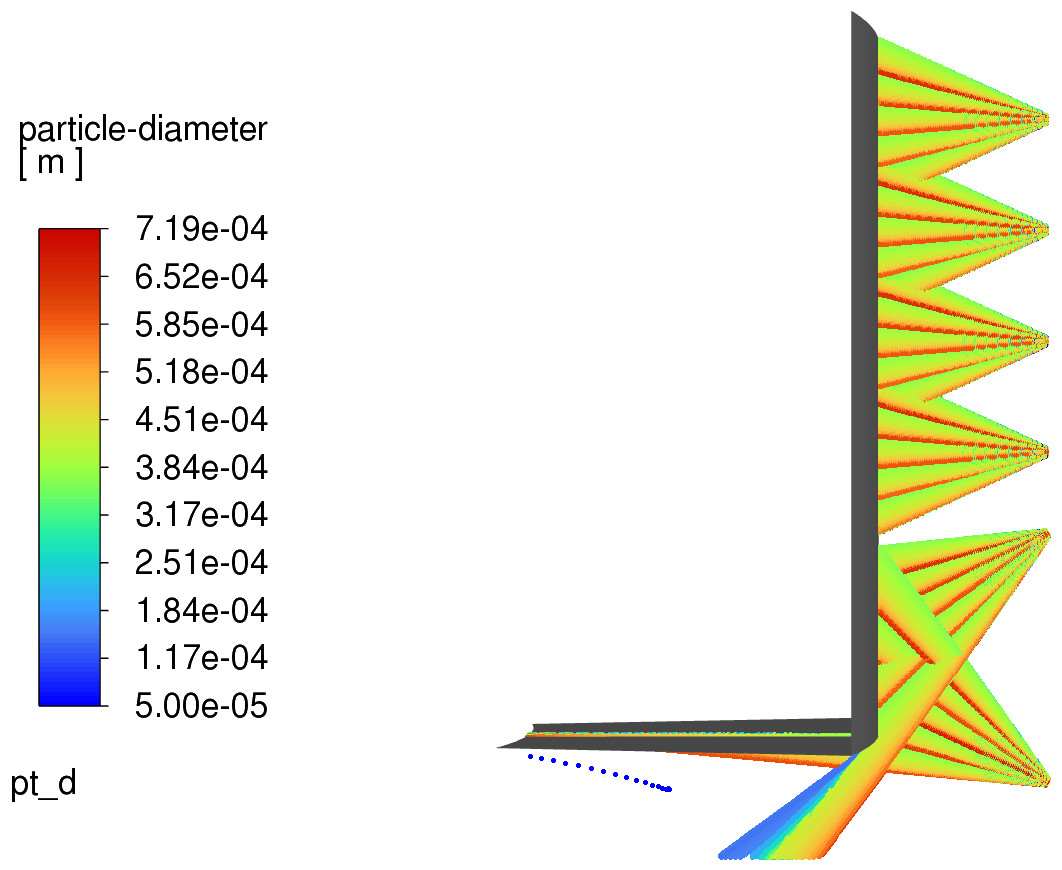
\includegraphics[width=0.62\textwidth]{fluent_gotas_od_cara_inferior.png}
\caption{Trayectorias de las gotas de las boquillas laterales e inferior exterior de un brazo sobre el diámetro exterior y la cara inferior, vista lateral, configuración base. La escala de color es el diámetro de la gota en metros (rótulo del programa en inglés). Imagen cualitativa: muestra la forma de los abanicos, no la dosis. Elaboración propia, simulación en ANSYS Fluent 2026 R1 (licencia Student); imagen recortada al área de interés.}
\label{fig:cfd-trayectorias}
\end{figure}

Ninguna superficie presentó zona seca con bandas de 10 mm. Con bandas de 2 mm, el diámetro exterior tuvo una franja de 0,39\,\% sin impacto directo entre $Z\approx1032$ y 1038 mm: el aire arrastrado por el chorro lateral más bajo desviaba hacia abajo las gotas de la boquilla inferior exterior. El acceso geométrico de las cuatro superficies fue de 99,13\,\% del área de referencia de 5,64 m$^2$; los 0,049 m$^2$ restantes son las huellas supuestas de los apoyos sectoriales (0,042 m$^2$) y la franja de los topes (0,007 m$^2$), que se asignan a la segunda etapa de lavado. Del caudal total de 202,59 L/min, el 52,1\,\% llegó al diámetro exterior, el 23,5\,\% al agujero, el 17,8\,\% a la cara superior, el 4,7\,\% a la cara inferior y el 2,0\,\% escapó.

La cara inferior es la superficie crítica. Recibió unas cuatro veces menos dosis que las demás, con la menor uniformidad y una transferencia del 31\,\%. Las gotas llegaban casi rasantes, con velocidades normales de 4,4 y 9,7 m/s frente a unos 23 m/s en las otras superficies, y su impulso era de diez a catorce veces menor. Ese resultado llevó a rediseñar las boquillas inferiores.

\subsubsection{Rediseño del diámetro exterior}

Para cerrar la franja del diámetro exterior se evaluaron dos variantes con el mismo caudal y el mismo número de boquillas. La primera inclina $-4^\circ$ la primera boquilla lateral de cada brazo; la segunda añade un desplazamiento de 15 mm hacia fuera de la segunda boquilla superior. La comparación se hizo frente a la configuración base con el brazo A duplicado, cuya franja seca de 2 mm es de 1,17\,\% (Tabla~\ref{tab:rediseno-od}).

\begin{table}[htbp]
\centering\small\singlespacing
\caption{Variantes de las boquillas del diámetro exterior y de la cara superior}
\label{tab:rediseno-od}
\begin{tabularx}{\textwidth}{@{}Yccc@{}}
\toprule
\textbf{Superficie e indicador} & \textbf{Base emparejada} & \textbf{Lateral inclinada} & \textbf{Más superior desplazada}\\
\midrule
Diámetro exterior: zona seca, bandas de 2 mm (\%) & 1,17 & 0 & 0\\
Diámetro exterior: CV, bandas de 10 mm & 0,304 & 0,265 & 0,265\\
Diámetro exterior: $D_{mín}$, bandas de 10 mm & 0,27 & 14,6 & 14,6\\
Cara superior: CV, bandas de 10 mm & 0,396 & 0,396 & 0,321\\
Cara superior: $D_{mín}$, bandas de 10 mm & 6,13 & 6,13 & 14,0\\
Cara superior: $\eta$ (\%) & 97,9 & 97,9 & 94,8\\
\bottomrule
\end{tabularx}
\par\smallskip\footnotesize
$D$ en kg\,m$^{-2}$ por vuelta. Ninguna de las dos variantes cambió la cara inferior.
\end{table}

La inclinación de la boquilla lateral basta para cerrar la franja y elevar la dosis mínima del diámetro exterior de 0,27 a 14,6 kg\,m$^{-2}$ por vuelta, sin costo de caudal; por eso se incorporó al diseño. El desplazamiento de la boquilla superior mejora además la cara superior, pero baja su transferencia en 3,1 puntos y no se incorporó al modelo CAD; queda como mejora evaluada.

\subsubsection{Configuración inferior propuesta}

La configuración de la Sección~\ref{sec:configuracion-inferior}, con 24 boquillas y la boquilla lateral inclinada, se simuló con los dos brazos explícitos, en la misma malla y con el mismo modelo que la configuración base. Las demás superficies conservaron sus resultados, porque la presión de sus boquillas cambió menos de 10 mbar. La Tabla~\ref{tab:cfd-propuesta} y la Figura~\ref{fig:cfd-propuesta} resumen los resultados.

\begin{table}[htbp]
\centering\small\singlespacing
\caption{Resultados del CFD de la configuración propuesta frente a la configuración base}
\label{tab:cfd-propuesta}
\begin{tabularx}{\textwidth}{@{}Yrrl@{}}
\toprule
\textbf{Indicador (dosis en kg\,m$^{-2}$ por vuelta)} & \textbf{Base*} & \textbf{Propuesta} & \textbf{Cambio}\\
\midrule
Cara inferior: dosis media & 5,46 & 14,16 & $\times2{,}6$\\
Cara inferior: coeficiente de variación & 0,626 & 0,430 & mejora\\
Cara inferior: dosis mínima, banda de 10 mm & 2,83 & 7,33 & $\times2{,}6$\\
Cara inferior: transferencia (\%) & 30,9 & 48,2 & $+17$ puntos\\
Zona exterior de la cara (Z3): dosis media & 4,1 & 19,99 & criterio 15,8\\
Zona exterior de la cara (Z3): coeficiente de variación & 0,246 & 0,298 & criterio $\leq0{,}4$\\
Diámetro exterior: dosis media & 26,38 & 25,82 & $-2{,}1$\,\%\\
Diámetro exterior: zona seca, bandas de 2 mm (\%) & 1,17 & 0 & se cierra\\
Cara inferior: tiempo de lavado con 183 kg\,m$^{-2}$, peor banda de 10 mm & 36,7 min & 14,7 min & 2,5 veces menos\\
\bottomrule
\end{tabularx}
\par\smallskip\footnotesize
*Base emparejada, con el brazo A duplicado; el tiempo base usa la dosis mínima de la Tabla~\ref{tab:cfd-caso-base} (2,93). Z3 es la zona de la cara inferior del aro exterior, entre los radios de 617,5 y 710 mm. El tiempo de lavado supone una dosis requerida de 183 kg\,m$^{-2}$ y 1,7 rpm, ambas hipótesis.
\end{table}

\begin{figure}[htbp]
\centering
\begin{minipage}[t]{0.49\textwidth}\centering
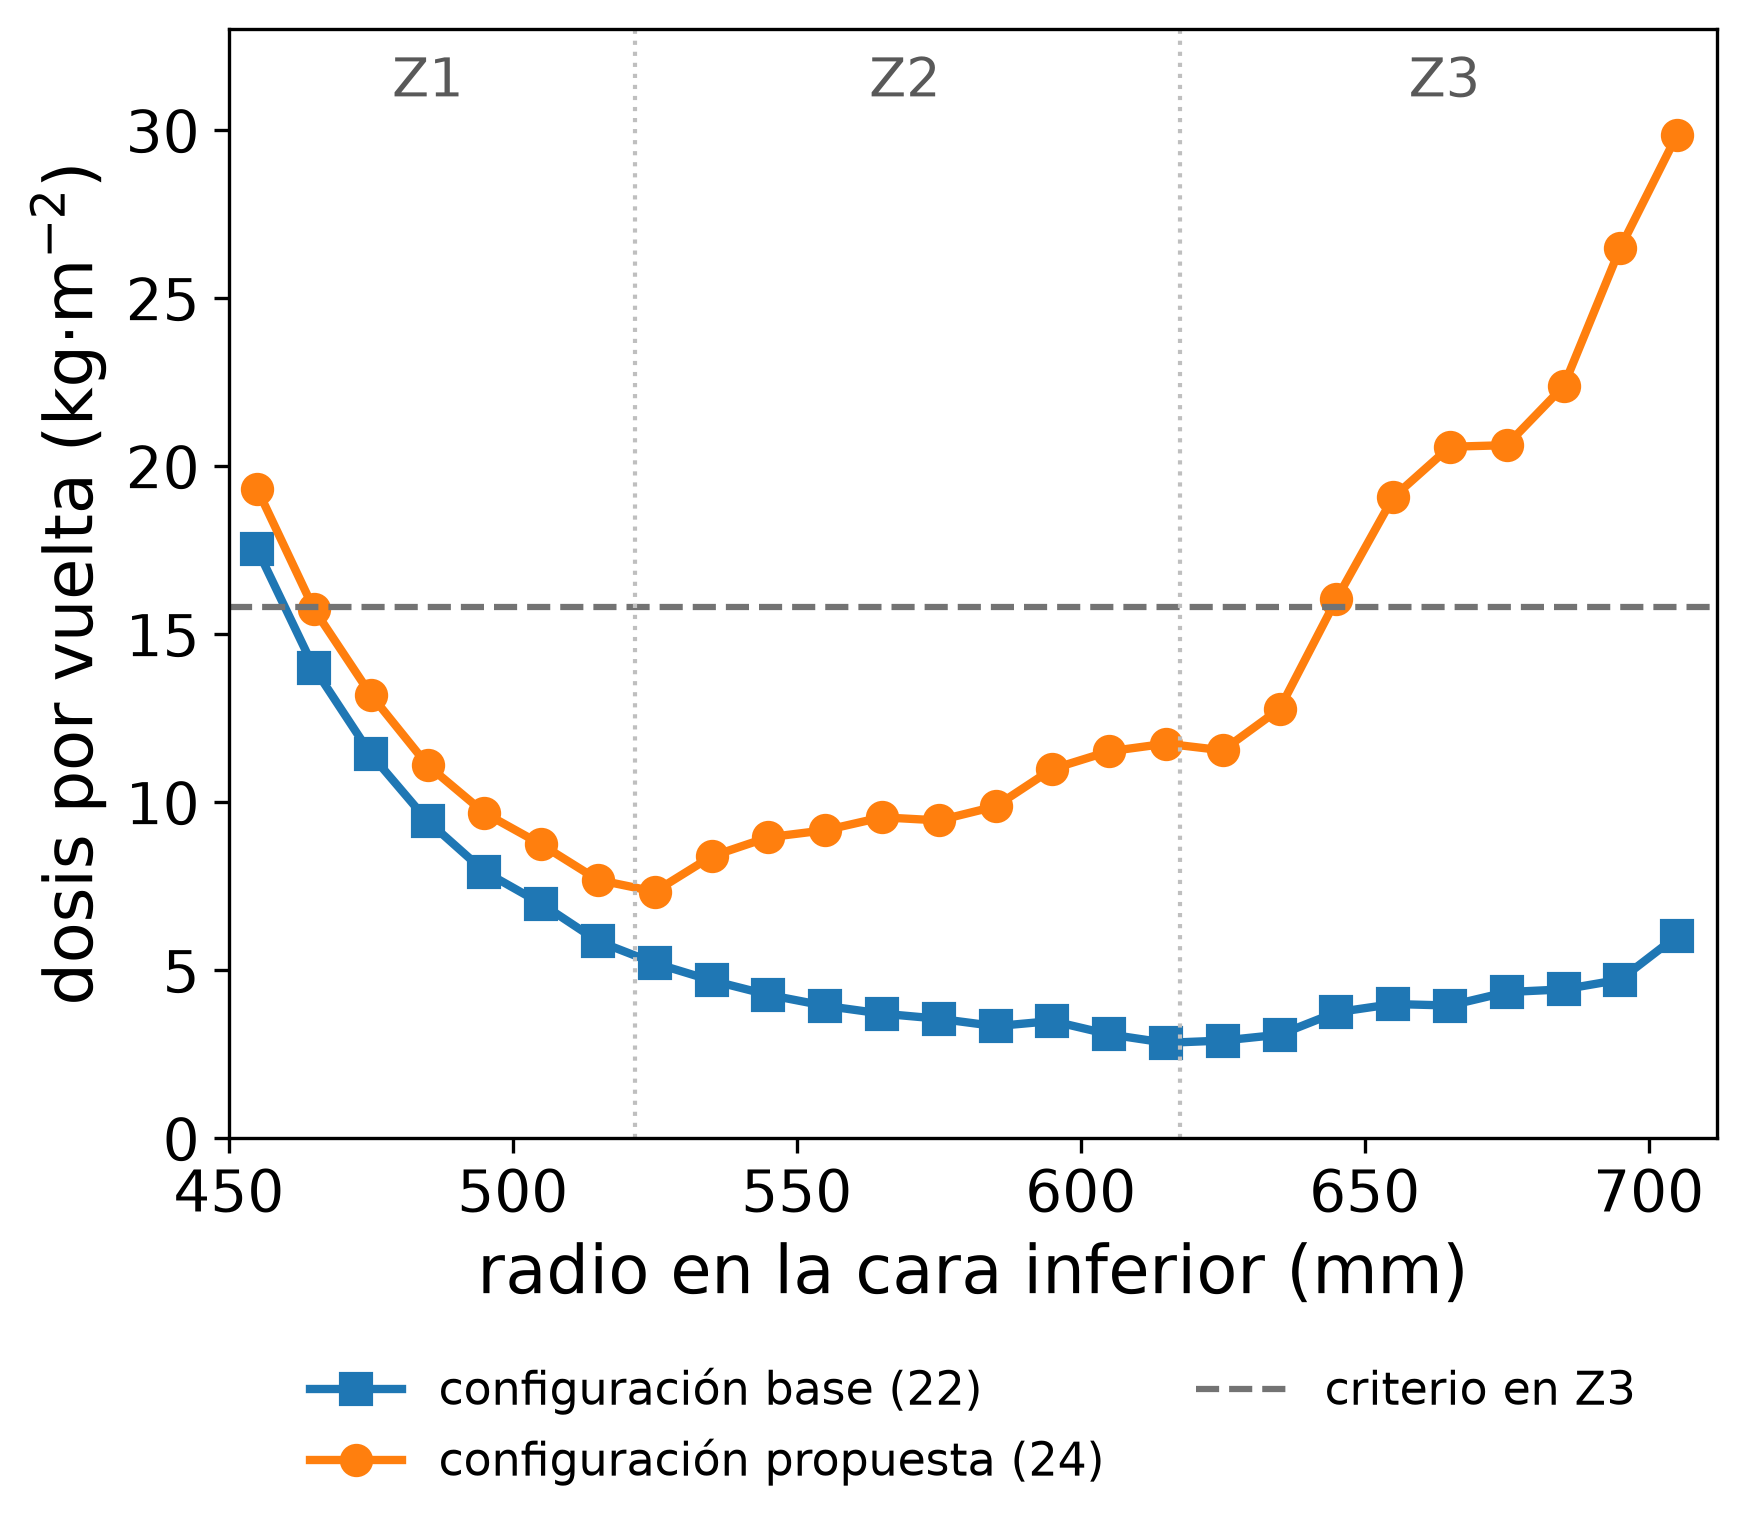
\includegraphics[width=\linewidth]{fig_dosis_cara_inferior.png}\par\small (a)
\end{minipage}\hfill
\begin{minipage}[t]{0.49\textwidth}\centering
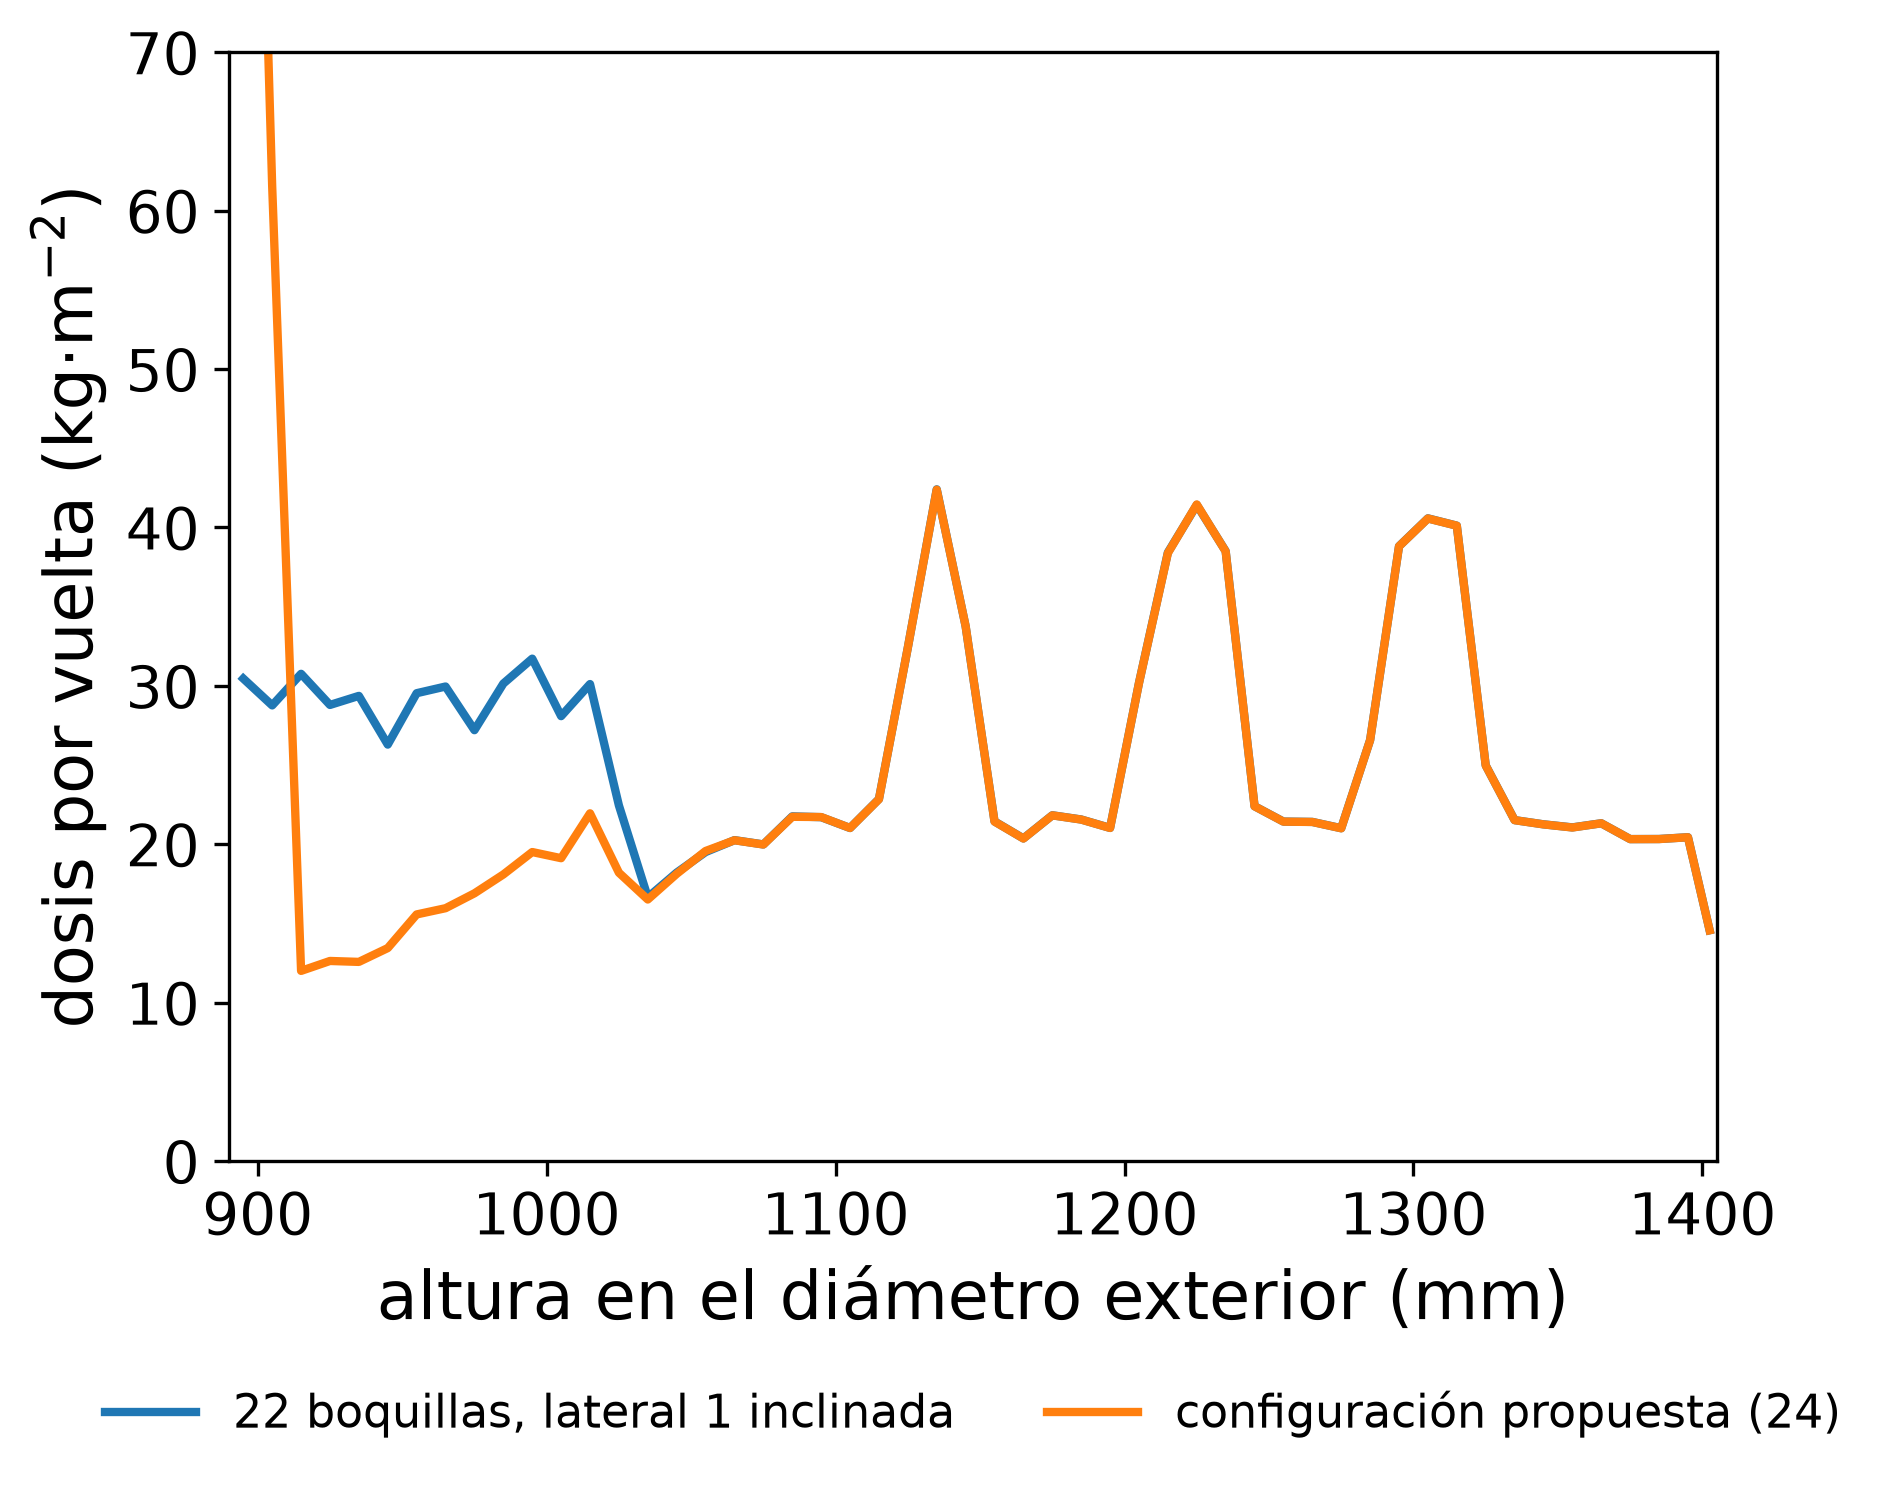
\includegraphics[width=\linewidth]{fig_dosis_diametro_exterior.png}\par\small (b)
\end{minipage}
\caption{Dosis por vuelta en bandas de 10 mm, con obstáculos: (a) cara inferior según el radio, con sus zonas Z1 (aro interior), Z2 (entre aros) y Z3 (aro exterior); (b) diámetro exterior según la altura. Elaboración propia con los datos exportados de ANSYS Fluent.}
\label{fig:cfd-propuesta}
\end{figure}

El par de boquillas inferiores cumple el criterio en la zona exterior de la cara inferior, con 19,99 frente a 15,8 kg\,m$^{-2}$ por vuelta y un coeficiente de variación de 0,298 frente a 0,4. La relación de dosis entre el diámetro exterior y la cara inferior baja de 4,8 a 1,8, y el tiempo de lavado de la cara inferior, medido en su peor banda, pasa de 36,7 a 14,7 min. Con dosis requeridas de 65 y 305 kg\,m$^{-2}$, sería de 5,2 y 24,5 min. Con ese criterio, la cara superior, cuya boquilla desplazada no se incorporó, necesita 17,6 min y es la que fija el tiempo de la máquina. Como la meta se cumplió, la reserva de elevar 25 mm los apoyos no hizo falta. El trazado de rayos había anticipado bien el resultado: esperaba de 19,6 a 19,7 en la zona exterior y el CFD dio 20,0, un 1,4\,\% más.

El cambio tiene un costo en el diámetro exterior. Las boquillas nuevas concentran agua en su borde inferior, con hasta 124 kg\,m$^{-2}$ por vuelta, y entre las alturas de 910 y 1000 mm la dosis baja de unos 29 a entre 12 y 20 (Figura~\ref{fig:cfd-propuesta}b). Frente a la configuración con la lateral inclinada, el coeficiente de variación del diámetro exterior sube de 0,265 a 0,648 y su dosis mínima baja de 14,56 a 10,53. La superficie sigue mojada por completo. Se definió para ella un criterio propio: sin zona seca y con una dosis mínima no menor que la de la superficie que fija el tiempo. Se cumple, con 0\,\% y 10,53 frente a 6,13 de la cara superior (7,33 en la cara inferior).

La verificación numérica usó tres mallas, de 202\,616, 430\,560 y 846\,960 celdas, con el número de Courant de gota cerca de 0,339 en las tres. Las dosis medias cambiaron como máximo un 0,63\,\% entre la malla base y la fina, y un 0,42\,\% al cambiar el número de parcelas (Figura~\ref{fig:cfd-malla-propuesta}); los balances de masa quedaron entre 0,024 y 0,125\,\%. No todo cumple el 2\,\%: las dosis mínimas de la cara inferior cambiaron entre 2,2 y 2,6\,\%. El orden de convergencia observado no es estable, porque algunas secuencias oscilan.

\begin{figure}[htbp]
\centering
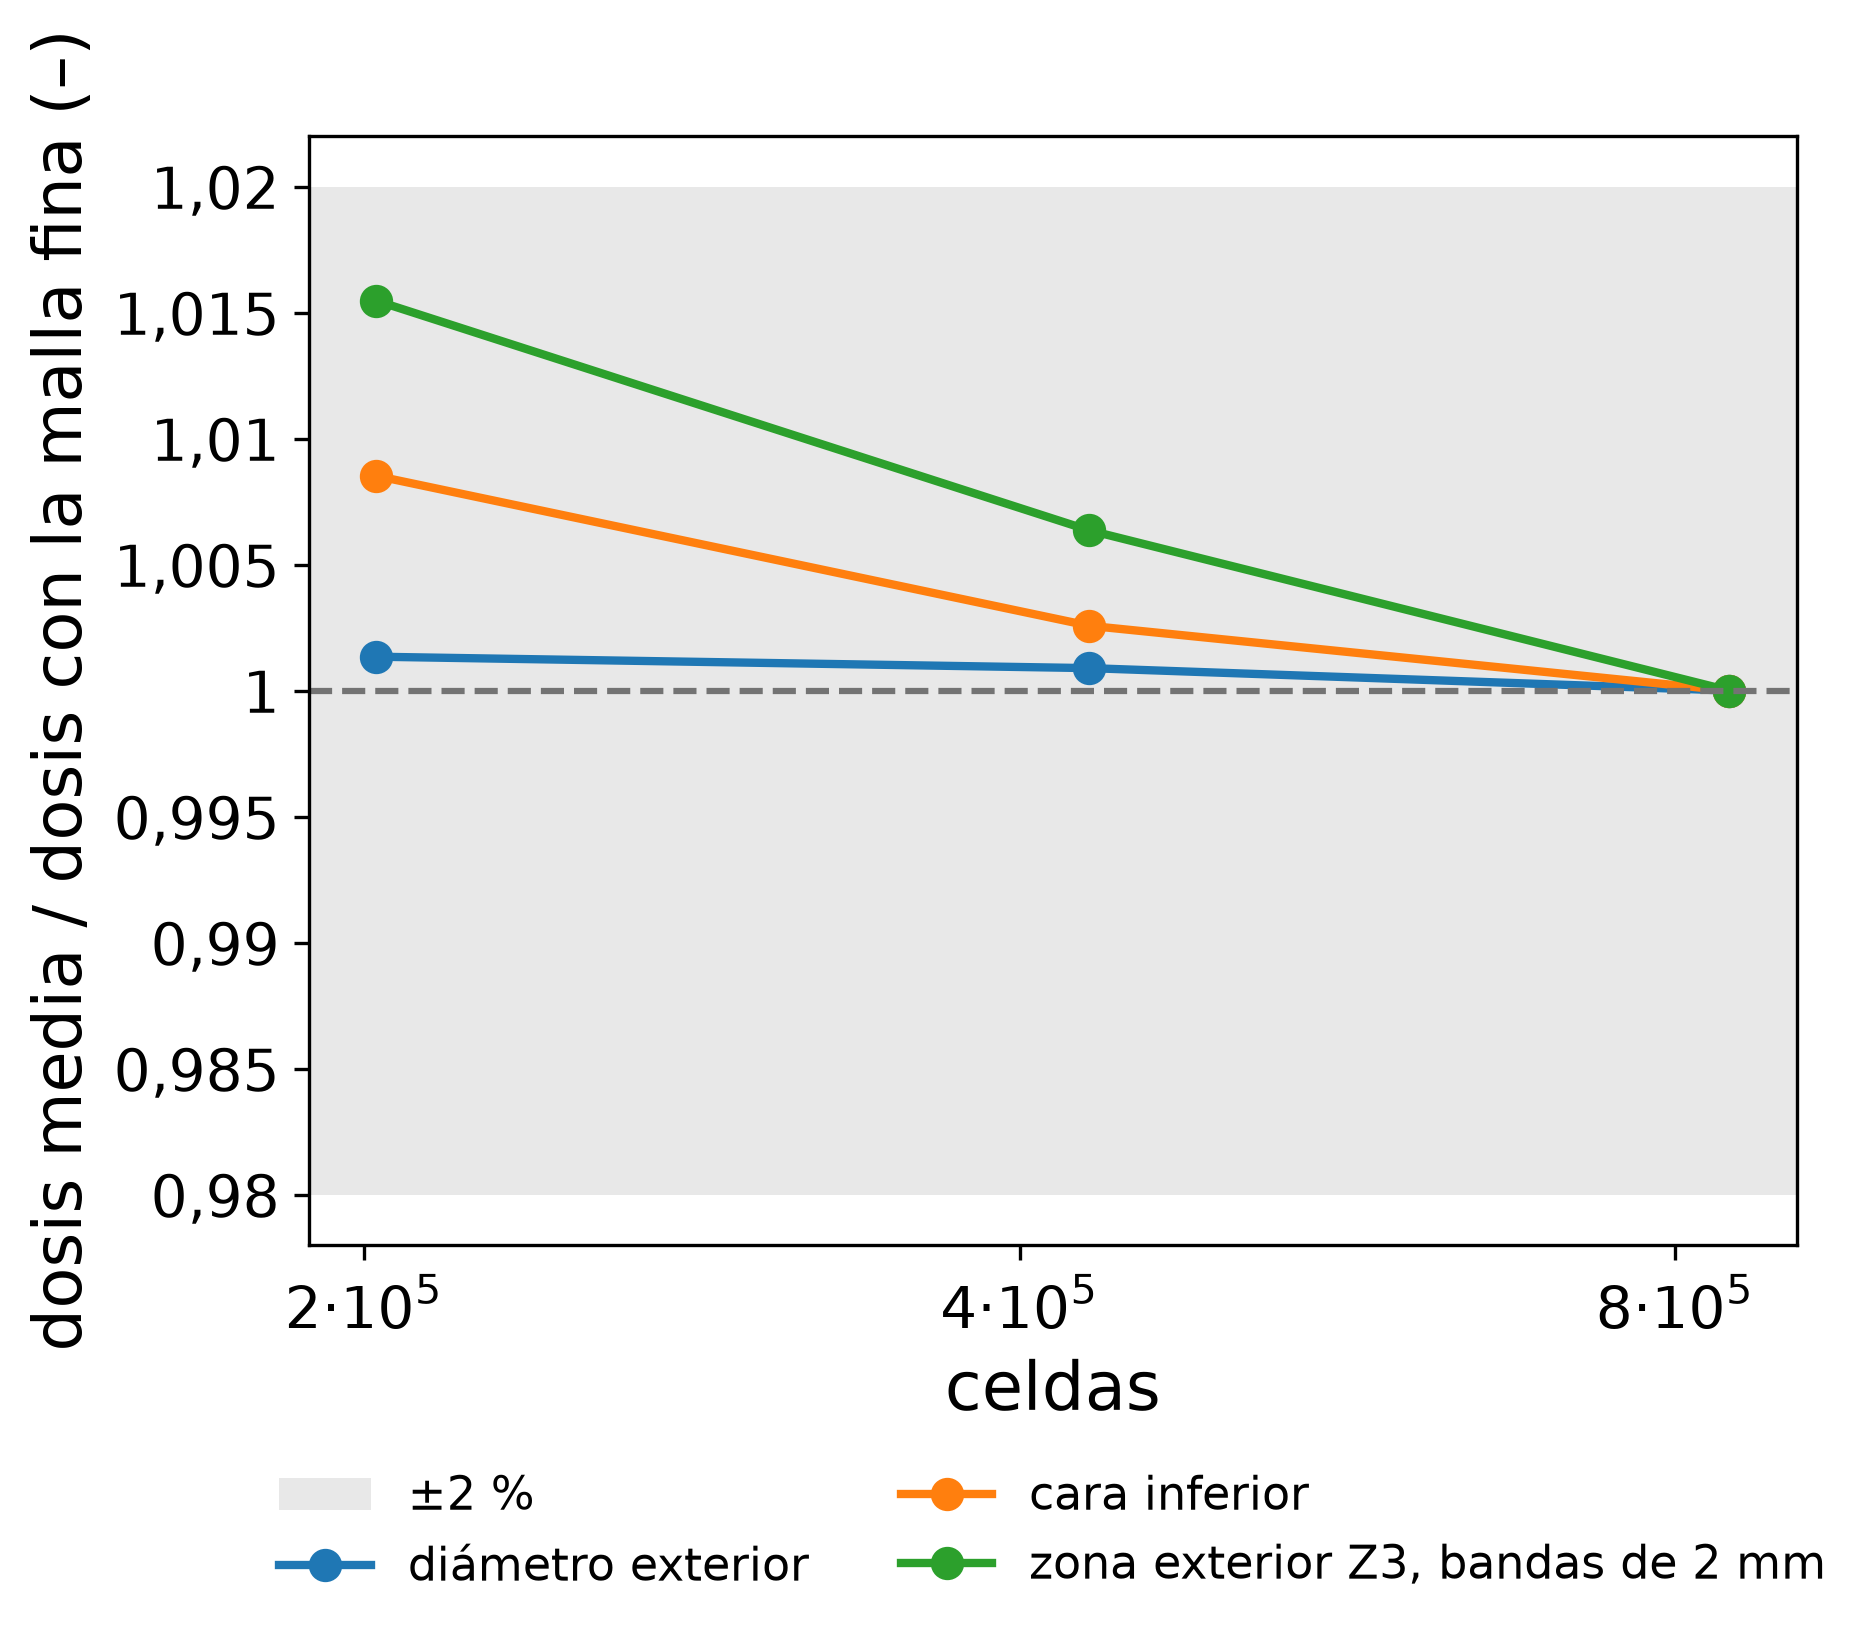
\includegraphics[width=0.55\textwidth]{fig_malla_configuracion_propuesta.png}
\caption{Dosis media de la configuración propuesta con tres mallas, normalizada con la de la malla fina. Elaboración propia con los datos exportados de ANSYS Fluent.}
\label{fig:cfd-malla-propuesta}
\end{figure}

\subsubsection{Alcance del lavado con el rodamiento armado}
\label{sec:alcance-lavado}

El lavado tiene por objetivo dejar el rodamiento en condiciones para la inspección visual inicial (Capítulo~\ref{cap:introduccion}). Su duración se estimó con el tiempo $t_{95}$ en que el 95\,\% del área accesible de cada superficie acumula una dosis requerida hipotética $D_{req}$ de 65, 183 o 305 kg\,m$^{-2}$, con la cara inferior leída por bandas de 10 mm y por celdas de 10 mm $\times$ 0,5$^\circ$, que registran las sombras parciales del soporte (Tabla~\ref{tab:tiempo-lavado}).

Con 183 kg\,m$^{-2}$, el diámetro exterior y el agujero llegan en 8,2 min y la cara superior en 10,6 min. Con el criterio del 95\,\% del área, la que más tarda es la cara inferior: con la dosis media de cada banda tarda de 5 a 24 min, pero las bases de los apoyos sectoriales y los topes dejan sombras parciales en un 14\,\% de su área, donde la dosis por vuelta es menor. Al resolver esas sombras por celdas, el tiempo sube a 27 y 76 min con 65 y 183 kg\,m$^{-2}$, y con 305 kg\,m$^{-2}$ no se alcanza en 120 min (Sección~\ref{sec:anx-tiempo-lavado}).

El lavado no alcanza el interior del rodamiento armado. Con la geometría de aros y rodillos medida en el modelo del fabricante y un trazado de rayos desde las 24 boquillas a lo largo de una vuelta del distribuidor, solo el 24\,\% del área de rodillos y pistas tiene línea de vista con alguna boquilla (Sección~\ref{sec:anx-cavidad}). La hilera inferior de rodillos queda casi oculta, con el 0,35\,\% de su superficie lateral visible, y la mitad inferior de las pistas, con el 2 al 16\,\%. Es una cota superior, porque el modelo no incluye la jaula. En ese espacio está la mayor parte de la grasa: según la regla del fabricante para el volumen libre \cite[p.~112]{skfgrasa}, el rodamiento lleno contiene de 84 a 89 kg, del mismo orden que los 75 kg de residuos por rodamiento que registra el taller (Capítulo~\ref{cap:introduccion}). El resultado cuantifica el alcance declarado: la máquina prepara las superficies exteriores para la inspección visual, y la limpieza de rodillos y pistas corresponde a la etapa con el rodamiento desarmado.

\subsection{Iteraciones de diseño}

Las iteraciones que condujeron a la configuración actual se ordenan en la Tabla~\ref{tab:iteraciones-resumen}; el registro detallado está en el Anexo~\ref{anx:iteraciones}.

\begingroup
\small\singlespacing
\setlength{\tabcolsep}{4pt}
\begin{longtable}{@{}>{\raggedright\arraybackslash}p{3.6cm}>{\raggedright\arraybackslash}p{\dimexpr(\textwidth-3.6cm-6\tabcolsep)/2\relax}>{\raggedright\arraybackslash}p{\dimexpr(\textwidth-3.6cm-6\tabcolsep)/2\relax}@{}}
\caption{Iteraciones principales del diseño}\label{tab:iteraciones-resumen}\\
\toprule
\textbf{Cambio} & \textbf{Hallazgo que lo motivó} & \textbf{Resultado}\\
\midrule\endfirsthead
\toprule
\textbf{Cambio} & \textbf{Hallazgo que lo motivó} & \textbf{Resultado}\\
\midrule\endhead
\bottomrule\endlastfoot
Mesa circular a bastidor de perfiles rectos & Muchas piezas e interfaces; ruedas en voladizo & Ruedas bajo las almas, sin ménsulas\\
Centradores de carro radial a brazo pivotante & Atravesaban los perfiles e invadían el rodamiento & Selección multicriterio: brazo pivotante\\
Uniones a momento diseñadas & La torsión de los travesaños gobernaba el centrado & Error de colocación de 3,35 mm con alas continuas\\
Límite de fuerza al empujador y ajuste H7/g6 & Error de 6,10 mm en la envolvente & 4,09 y 4,24 mm en los estados de operación\\
Rueda de 200 mm revisada & Se comparaba la carga última con la capacidad de rodadura & D/C 0,89 y 0,43; se descartó la de 250 mm\\
Empuje manual a doble cadena con volante & 325 a 837 N de empuje y 565 N de frenado & 15,5 a 39,8 N en el volante; parada con 190 N\\
Cabezal sobre monorriel a U superior giratoria con lanza & Movimiento y acceso del aplicador & Rodamiento y mesa inmóviles en el lavado\\
19 a 22 boquillas & Sin aplicación hacia la cara inferior & Acceso de 99,1\,\% por trazado de rayos\\
Lateral 1 inclinada $-4^\circ$ & Franja seca de 2 mm en el diámetro exterior & Sin zona seca\\
22 a 24 boquillas, par inferior estrecho & Cara inferior con cuatro veces menos dosis & Zona exterior de 4,1 a 20,0 kg\,m$^{-2}$ por vuelta\\
Masa del rotor medida en el CAD & La envolvente de 180 kg no cubría el rotor real & 231 kg; eje con D/C 0,27\\
Soporte superior aligerado & El criterio anterior no era funcional & De 360 a 247 kg con criterios de rigidez\\
\end{longtable}
\endgroup

\subsection{Limitaciones de los resultados}

Cada limitación que condiciona la interpretación de los resultados figura en la Tabla~\ref{tab:limitaciones-resultados} junto con la acción prevista.

\begingroup
\small\singlespacing
\setlength{\tabcolsep}{4pt}
\begin{longtable}{@{}>{\raggedright\arraybackslash}p{2.8cm}>{\raggedright\arraybackslash}p{\dimexpr(\textwidth-2.8cm-6\tabcolsep)*58/100\relax}>{\raggedright\arraybackslash}p{\dimexpr(\textwidth-2.8cm-6\tabcolsep)*42/100\relax}@{}}
\caption{Limitaciones de los resultados y acciones previstas}\label{tab:limitaciones-resultados}\\
\toprule
\textbf{Resultado} & \textbf{Limitación y efecto} & \textbf{Acción}\\
\midrule\endfirsthead
\caption[]{Limitaciones de los resultados y acciones previstas (continuación)}\\
\toprule
\textbf{Resultado} & \textbf{Limitación y efecto} & \textbf{Acción}\\
\midrule\endhead
\midrule\multicolumn{3}{r}{\textit{Continúa en la página siguiente.}}\\\endfoot
\bottomrule\endlastfoot
Análisis estructural & Apoyos bilaterales; el desvío lateral se aplicó entero a una sola rueda, lo que es conservador & Modelo con apoyo unilateral\\
Uniones y centrado & Continuidad perfecta de alas supuesta; partidas de tolerancia sin medición; disparo del limitador sin calibrar & Medición de referencias, juegos y fuerza del limitador\\
Red hidráulica & Coeficientes de pérdida estimados; altura de 53,39 o 51,0--51,3 m según el trazado; curva de la bomba leída del gráfico & Curva del fabricante y medición de presión por boquilla\\
Modelo de mojado & Retención en el primer impacto: dosis y transferencia son cotas superiores; inyección y 1,7 rpm supuestas; rodamiento con el extremo menor del agujero hacia abajo; la boquilla inferior adicional envía del 16 al 17\,\% de su caudal hacia el agujero, y que el agujero no cambie es una hipótesis & Sensibilidad a la inyección y a la orientación; corrida del agujero con la configuración propuesta\\
Limpieza & No se calcula la remoción; el VOF acota el cortante en la pared entre 5 Pa y 2 kPa (Sección~\ref{sec:anx-vof}); la dosis requerida es una hipótesis & Ensayos de huella y de remoción\\
Interior del rodamiento & 24\,\% de rodillos y pistas visible, sin la jaula & Limpieza con el rodamiento desarmado\\
Distribuidor y soporte & Tiro de la correa, carga accidental y presión supuestos; bases tomadas como empotradas & Selección de catálogo y detalle de las bases\\
Sismo & Revisión estática; la viga bajo los topes puede fluir localmente en un sismo severo & Modelo local por elementos finitos\\
\end{longtable}
\endgroup

\section{Verificación del cumplimiento de las especificaciones técnicas}
\label{sec:verificacion-especificaciones}

La Tabla~\ref{tab:cumplimiento-especificaciones} contrasta las especificaciones E01--E15 de la Tabla~\ref{tab:especificaciones_revision} con los resultados. «Cumple en el modelo» indica que el resultado numérico satisface el criterio dentro de las hipótesis del modelo.

\begingroup
\small\singlespacing
\setlength{\tabcolsep}{3pt}
\renewcommand{\arraystretch}{1.08}
\begin{longtable}{@{}p{0.75cm}>{\raggedright\arraybackslash}p{3.1cm}>{\raggedright\arraybackslash}p{4.9cm}>{\raggedright\arraybackslash}p{\dimexpr\textwidth-8.75cm-8\tabcolsep\relax}@{}}
\caption{Matriz de cumplimiento de especificaciones}\label{tab:cumplimiento-especificaciones}\\
\toprule
\textbf{Cód.} & \textbf{Criterio} & \textbf{Resultado} & \textbf{Estado}\\
\midrule\endfirsthead
\caption[]{Matriz de cumplimiento de especificaciones (continuación)}\\
\toprule
\textbf{Cód.} & \textbf{Criterio} & \textbf{Resultado} & \textbf{Estado}\\
\midrule\endhead
\midrule\multicolumn{4}{r}{\textit{Continúa en la página siguiente.}}\\\endfoot
\bottomrule\endlastfoot
E01 & Admitir 1420/900/515 mm & Envolvente en el CAD sin interferencias; paso por la puerta modelada & Cumple en el modelo; maniobra de planta pendiente\\
E02 & 3032 kg y pesos separados & 29,84 kN en los apoyos sectoriales; masa móvil de 3440 kg frente a 3500 kg de diseño & Cumple\\
E03 & Flecha $\leq L/800$ & 1,236 mm frente a 2,33 mm (también $<L/1000$) & Cumple en el nodo evaluado\\
E04 & D/C $\leq1$ & Barras del bastidor 0,82; uniones 0,58; distribuidor 0,93; soporte superior 0,18 & Cumple en el modelo\\
E05 & Reacciones compresivas sin amarre & Apoyos sectoriales y ruedas con reacciones no negativas; los pedestales del riel se anclan para $-3{,}78$ kN & Cumple en cálculo; losa por confirmar\\
E06 & Error de colocación $\leq5$ mm & 4,09 y 4,24 mm con alabeo libre; 3,35 mm con alas continuas; envolvente de 2,08 kN: 3,91 mm con alas continuas & Cumple con la fuerza final limitada a 1,95 kN\\
E07 & Carga exterior y mesa inmovilizada & Recorrido de 3320 mm; pasador con ajuste H7/g6 en carga y lavado; cadena entre estaciones & Cumple en diseño; enclavamiento en el Capítulo~\ref{cap:seguridad-ambiente}\\
E08 & Captura $\geq5$ mm & 13,1 mm en el peor caso; carrera base de 6,6 mm & Cumple numéricamente\\
E09 & 4--6 bar en la boquilla & 4,00--4,13 bar & Cumple en el modelo\\
E10 & $\leq8$ bar & Máximo de 4,13 bar & Cumple en el modelo\\
E11 & 1--3 m/s en la impulsión & 2,57 m/s en DN40 (cálculo); 1,56 m/s en DN50 (trazado) & Cumple en el modelo\\
E12 & 1--2 rpm; 30--60 s por vuelta & 1,7 rpm; 35,3 s & Valor de diseño; no medido\\
E13 & Cobertura $\geq80$\,\% (objetivo 95\,\%) & Acceso de 99,13\,\%; sin zona seca en bandas de 10 mm, ni en bandas de 2 mm del diámetro exterior con 24 boquillas & Cumple en el modelo\\
E14 & Drenaje $\geq250$ L/min & Captación de 333--350 L/min con 50\,\% de obstrucción; línea por gravedad de 413 L/min & Cumple en cálculo\\
E15 & Holgura positiva mesa--distribuidor & 18,8 mm nominal; barrido del traslado sin choques & Cumple en el CAD nominal\\
\end{longtable}
\endgroup

De las quince especificaciones, catorce se satisfacen en los modelos y en los cálculos; la velocidad del distribuidor es un valor de diseño que no se puede verificar sin el equipo. La precisión de centrado, que no se cumplía en la segunda entrega, se cumple ahora porque se limitó la fuerza del empujador y se dio continuidad a las alas del bastidor. Ninguna especificación se verificó con ensayos.

\section{Verificación del cumplimiento de restricciones}
\label{sec:verificacion-restricciones}

La Tabla~\ref{tab:cumplimiento-restricciones} verifica la configuración frente a las restricciones RS-01--RS-12 del Capítulo~\ref{cap:marco-referencial}. «Condicionada» indica que la restricción se satisface en el diseño, pero su comprobación depende de datos externos o de la implementación.

\begingroup
\small\singlespacing
\setlength{\tabcolsep}{3.5pt}
\renewcommand{\arraystretch}{1.08}
\begin{longtable}{@{}p{1.1cm}>{\raggedright\arraybackslash}p{2.6cm}>{\raggedright\arraybackslash}p{\dimexpr\textwidth-1.1cm-2.6cm-4.0cm-8\tabcolsep\relax}>{\raggedright\arraybackslash}p{4.0cm}@{}}
\caption{Verificación de restricciones}\label{tab:cumplimiento-restricciones}\\
\toprule
\textbf{Cód.} & \textbf{Restricción} & \textbf{Comprobación} & \textbf{Resultado}\\
\midrule\endfirsthead
\caption[]{Verificación de restricciones (continuación)}\\
\toprule
\textbf{Cód.} & \textbf{Restricción} & \textbf{Comprobación} & \textbf{Resultado}\\
\midrule\endhead
\midrule\multicolumn{4}{r}{\textit{Continúa en la página siguiente.}}\\\endfoot
\bottomrule\endlastfoot
RS-01 & Seguridad laboral & Secuencia que separa izaje, centrado, traslado y aspersión; traslado sin empuje directo; enclavamientos definidos (Capítulo~\ref{cap:seguridad-ambiente}) & Pasa en diseño; implementación pendiente\\
RS-02 & Técnica: masa y geometría & E01 y E02 & Pasa\\
RS-03 & Preservación & Contacto solo en superficies autorizadas; presión media de 0,85 MPa en los apoyos; presión máxima de 4,13 bar en las boquillas & Pasa en el modelo; revestimiento por confirmar con el fabricante\\
RS-04 & Espacial & Recorrido y paso por la puerta modelados & Condicionada al levantamiento del taller\\
RS-05 & Infraestructura & Pedestales anclados para levantamiento, guiado y tensor de las cadenas, con losa supuesta de 200 mm & Condicionada a la losa real\\
RS-06 & Geográfica y ambiental & Escenario de 2335 m para presión atmosférica y NPSH; zona sísmica supuesta & Condicionada a la ficha del emplazamiento\\
RS-07 & Servicios & Bomba de 4 kW, resistencias de 36 kW y circuito recirculado de 221 L/min & Pendiente de datos del taller\\
RS-08 & Ambiental y legal & Contención en cabina, pozo de drenaje y contenedor de 1000 L para la purga & Parcial; destino del efluente por definir\\
RS-09 & Química y ocupacional & Agua con detergente alcalino de baja espuma, compatible con acero y latón \cite{zep36342} & Pasa en diseño\\
RS-10 & Económica y constructiva & Presupuesto de clase 4 de S/~319\,095 sin IGV (Capítulo~\ref{cap:cronograma-presupuesto}) & No evaluable como filtro: no hay techo acreditado\\
RS-11 & Organizacional y ergonómica & Fuerza de 15,5 a 39,8 N en el volante, frente a 325--837 N de empuje directo & Pasa en cálculo; evaluación ergonómica con fuerzas medidas pendiente \cite{iso11228}\\
RS-12 & Propiedad industrial & Revisión de antecedentes conservada & Pendiente de evaluación de libertad de operación\\
\end{longtable}
\endgroup

La configuración no incumple ninguna restricción identificada, pero solo la técnica pasa sin condiciones. Las demás dependen de datos del taller, de la implementación de los controles o de ensayos. El sistema de soporte y el de aspersión quedan definidos como candidatos verificados por simulación y cálculo, no validados experimentalmente.

\chapter{ANÁLISIS DE SEGURIDAD, RIESGOS E IMPACTOS AMBIENTALES}
\label{cap:seguridad-ambiente}

\section{Consideraciones de seguridad y análisis de riesgos}

El análisis siguió la estrategia de ISO 12100: se fijaron los límites de la máquina, se identificaron los peligros en cada estado de operación, se estimó el riesgo y se aplicaron las medidas en tres pasos, primero por diseño intrínsecamente seguro, después con medidas de protección y, por último, con información para la utilización \cite{iso12100}. La serie EN 12921 se usó para reconocer los peligros propios de las máquinas de limpieza con líquidos acuosos \cite{en12921_1,en12921_2}, y el reglamento de seguridad minera fija la obligación de identificar peligros y controlar cada tarea \cite{ds024}. La mención de estas normas no equivale a una declaración de conformidad.

Los límites de la máquina son los siguientes: un rodamiento de 3032 kg por ciclo, una masa móvil de diseño de 3500 kg, agua con detergente alcalino de baja espuma a 62~$^\circ$C y hasta 4,13 bar en las boquillas, un operador entrenado y personal de izaje del taller. Los estados de operación son los siete pasos de la Sección~\ref{sec:integracion}: carga y centrado en la estación exterior, traslado, bloqueo en la estación de lavado, precalentamiento y lavado con la cabina cerrada, enjuague, despresurización y retiro.

El diseño elimina o reduce varios peligros en su origen. La carga, el centrado y el retiro ocurren fuera de la cabina, separados de la aspersión. El rodamiento y la mesa permanecen inmóviles durante el lavado, de modo que el único movimiento en la cabina es el del distribuidor, que gira a 1,7 rpm con un limitador de par. La mesa se mueve con una cadena que impone su velocidad, sin empuje directo. El empujador del centrador se detiene por fuerza normal limitada, para no dañar el aro ni formar un camino rígido de carga. El fluido es acuoso, lo que excluye los peligros de los líquidos inflamables, y la presión de trabajo, de 4,13 bar como máximo, queda por debajo del límite de 8 bar fijado para preservar las pistas.

Para priorizar las medidas se usó una escala cualitativa de probabilidad $P$ y severidad $S$ de 1 a 4 (Tabla~\ref{tab:escala-riesgo}). El índice $R=P\,S$ ordena los controles; no acredita un riesgo residual aceptable. Los valores son una evaluación de diseño y deben revisarse con el responsable de seguridad del taller y con el procedimiento real.

\begin{table}[htbp]
\centering\small\singlespacing
\caption{Escala de probabilidad, severidad y nivel de riesgo}
\label{tab:escala-riesgo}
\begin{tabularx}{\textwidth}{@{}cYY@{}}
\toprule
\textbf{Valor} & \textbf{Probabilidad $P$} & \textbf{Severidad $S$}\\
\midrule
1 & Improbable durante la vida de la máquina & Lesión leve, sin pérdida de días\\
2 & Posible en condiciones anómalas & Lesión con descanso médico\\
3 & Probable en algún ciclo de operación o mantenimiento & Lesión grave o incapacidad temporal\\
4 & Frecuente si no hay control & Lesión incapacitante o mortal\\
\midrule
\multicolumn{3}{@{}l}{Nivel de riesgo: bajo para $R\leq4$; medio para $R=6$ u $8$; alto para $R\geq9$.}\\
\bottomrule
\end{tabularx}
\end{table}

La Tabla~\ref{tab:matriz-riesgos} presenta la matriz de peligros. Para cada uno se indican la medida preventiva y el paso de ISO 12100 al que pertenece (1: diseño intrínseco; 2: protección; 3: información y procedimiento), la medida de contingencia ante el evento y el riesgo residual esperado si las medidas se implementan y verifican.

\begingroup
\small\singlespacing
\setlength{\tabcolsep}{3pt}
\renewcommand{\arraystretch}{1.06}
\begin{longtable}{@{}>{\raggedright\arraybackslash}p{1.9cm}>{\raggedright\arraybackslash}p{2.6cm}>{\centering\arraybackslash}p{0.75cm}>{\raggedright\arraybackslash}p{\dimexpr\textwidth-1.9cm-2.6cm-0.75cm-2.6cm-1.7cm-10\tabcolsep\relax}>{\raggedright\arraybackslash}p{2.6cm}>{\raggedright\arraybackslash}p{1.7cm}@{}}
\caption{Matriz de peligros, medidas preventivas, contingencia y riesgo residual}\label{tab:matriz-riesgos}\\
\toprule
\textbf{Estado} & \textbf{Peligro y consecuencia} & \textbf{P--S (R)} & \textbf{Medida preventiva (paso)} & \textbf{Contingencia} & \textbf{Residual}\\
\midrule\endfirsthead
\caption[]{Matriz de peligros, medidas preventivas, contingencia y riesgo residual (continuación)}\\
\toprule
\textbf{Estado} & \textbf{Peligro y consecuencia} & \textbf{P--S (R)} & \textbf{Medida preventiva (paso)} & \textbf{Contingencia} & \textbf{Residual}\\
\midrule\endhead
\midrule\multicolumn{6}{r}{\textit{Continúa en la página siguiente.}}\\\endfoot
\bottomrule\endlastfoot
Izaje y carga & Caída o giro del rodamiento; aplastamiento & 2--4 (8) & Carga fuera de la cabina con pasador en la estación de carga (1); aparejo certificado y zona de exclusión (2); plan de izaje y señalero (3) & Suspender la maniobra, despejar la zona y apoyar la carga en lugar seguro & Medio\\
Centrado & Atrapamiento de manos entre aro, apoyo sectorial y centrador & 3--3 (9) & Empujador con fuerza normal limitada a 1,45 kN y disparo independiente a 1,60 kN (1); mando desde fuera del alcance (2); prohibición de intervenir en la interfaz (3) & Parada de emergencia y liberación manual del empujador & Medio\\
Traslado & Movimiento no controlado, choque o atrapamiento con la mesa cargada & 3--4 (12) & Doble cadena que impone 0,032 m/s y detiene la mesa con 190 N; rieles con pestaña (1); pasador fusible de 3 kN en el volante y zona de paso señalizada (2); operación desde el volante, fuera de la cabina (3) & Detener el volante e insertar el pasador de bloqueo; calzos en el riel & Bajo\\
Traslado con el distribuidor fuera de 0$^\circ$ & Choque entre mesa y distribuidor & 2--3 (6) & Traslado permitido solo con el distribuidor detenido a 0$^\circ$ y la lanza retirada, mediante enclavamiento (2) & Detención del traslado e inspección del distribuidor & Bajo\\
Bloqueo & Inicio de la aspersión con la mesa libre & 2--4 (8) & Pasador con receptor en la estación de lavado y confirmación positiva de posición (2) & Corte de la bomba y del giro & Bajo\\
Aspersión y giro & Golpe o arrastre por el distribuidor giratorio; descenso de la lanza sobre una persona & 2--4 (8) & Giro lento de 1,7 rpm y limitador de par de 30 N\,m en el motorreductor (1); cabina cerrada con puerta enclavada y sin personal dentro (2) & Parada de emergencia que detiene giro, lanza y bomba & Bajo\\
Giro del distribuidor & Atasco de la U con un objeto; rotura del eje del motorreductor & 2--3 (6) & Limitador de par, que desliza antes de que el eje llegue a su carga admisible (1); inspección del limitador (3) & Parada y retiro del objeto con la energía aislada & Bajo\\
Sismo & Deslizamiento del rodamiento sobre los apoyos; vuelco de la mesa & 1--4 (4) & Tres topes de retención con cartelas; mesa sin vuelco, con factores de 3,45 y 2,59 (1); inspección y reapriete después de un sismo severo (3) & Evacuar la cabina; inspeccionar topes, mordazas y viga bajo los topes & Bajo\\
Aspersión & Impacto del chorro o proyección de fluido caliente & 3--3 (9) & Presión de 4,13 bar como máximo (1); cabina cerrada (2); despresurización antes de abrir (3) & Lavado de ojos y piel; primeros auxilios según la hoja de seguridad & Bajo\\
Fluido & Quemadura a 62~$^\circ$C, contacto dérmico o inhalación de niebla alcalina & 3--3 (9) & Fluido acuoso (1); ventilación de la cabina (2); hoja de seguridad, equipo de protección y capacitación (3) & Ducha y lavaojos; atención médica & Medio\\
Drenaje & Derrame, resbalón o exposición al efluente & 3--3 (9) & Piso con pendiente, sumidero y cesta, captación superior a 250 L/min (1); alarma de nivel (2) & Kit antiderrames y contención secundaria & Bajo\\
Servicio técnico & Energía residual y movimiento inesperado & 2--4 (8) & Puntos de purga y despresurización (1); aislamiento, bloqueo y etiquetado (2); procedimiento escrito (3) & Liberación de energía según procedimiento & Bajo\\
Equipo eléctrico & Contacto eléctrico en ambiente húmedo & 2--4 (8) & Tablero fuera de la cabina con grado IP54, y motores y sensores de la zona húmeda con grado IP66; cables y bornes fuera del alcance de la aspersión (1); seccionador general bloqueable, protección diferencial de 30 mA y mando a 24 V (2); bloqueo y etiquetado antes de intervenir (3) & Apertura del seccionador general y atención de emergencia & Bajo\\
\end{longtable}
\endgroup
\noindent{\footnotesize Valoración de diseño con la escala de la Tabla~\ref{tab:escala-riesgo}.\par}

El traslado de la mesa cargada era el riesgo más alto de la segunda entrega, porque el empuje manual exigía de 325 a 837 N y la parada, 565 N. La doble cadena con volante lo reduce en su origen: la fuerza en la empuñadura queda entre 15,5 y 39,8 N, la cadena limita la velocidad a 0,032 m/s y la mesa se detiene con 190 N (Sección~\ref{sec:dimensionamiento-traslado}). El operador queda fuera de la cabina y lejos de la mesa. La evaluación ergonómica con fuerzas medidas según ISO 11228-2 \cite{iso11228} sigue pendiente.

La estabilidad del conjunto depende de que las reacciones de las ruedas permanezcan compresivas. La envolvente de tres contactos con reacciones no negativas dio 19,01 kN por rueda sin factor, y la carga resistente de rueda es de 26,62 kN. Las reacciones negativas del modelo continuo del riel, de hasta 3,78 kN, se resolvieron anclando los pedestales a la losa; en la revisión sísmica, la rueda menos cargada conservó 4,58 kN de compresión (Anexo~\ref{anx:calculos}).

El control funcional mínimo debe impedir la aspersión si la puerta está abierta, la mesa no está bloqueada en la estación de lavado o la lanza no está en su posición; impedir el traslado si el distribuidor no está detenido a 0$^\circ$ o la lanza no está retirada, y permitir la parada de emergencia y la descarga segura de la presión. La lógica de control, su nivel de desempeño y la arquitectura eléctrica no se diseñaron en este alcance y se tratan en las recomendaciones.

\section{Análisis de impactos ambientales y sostenibilidad}

Los aspectos ambientales del ciclo de lavado son el uso del fluido y de la energía, la generación de efluente con grasa y partículas, los residuos sólidos de mantenimiento, las emisiones de niebla y vapor, y los derrames. La Ley de Gestión Integral de Residuos Sólidos proporciona el marco para las corrientes de residuos \cite{dleg1278}; su clasificación concreta depende de la caracterización del contaminante, que es grasa con polvo mineral y posibles partículas de desgaste. La Tabla~\ref{tab:impactos-ambientales} resume los impactos por medio receptor.

\begingroup
\small\singlespacing
\setlength{\tabcolsep}{3.5pt}
\begin{longtable}{@{}>{\raggedright\arraybackslash}p{2.3cm}>{\raggedright\arraybackslash}p{\dimexpr(\textwidth-2.3cm-1.0cm-2.6cm-8\tabcolsep)/2\relax}>{\centering\arraybackslash}p{1.0cm}>{\raggedright\arraybackslash}p{\dimexpr(\textwidth-2.3cm-1.0cm-2.6cm-8\tabcolsep)/2\relax}>{\raggedright\arraybackslash}p{2.6cm}@{}}
\caption{Impactos ambientales y sociales del ciclo de lavado}\label{tab:impactos-ambientales}\\
\toprule
\textbf{Medio o aspecto} & \textbf{Impacto} & \textbf{Signo} & \textbf{Medida o cuantificación} & \textbf{Estado}\\
\midrule\endfirsthead
\caption[]{Impactos ambientales y sociales del ciclo de lavado (continuación)}\\
\toprule
\textbf{Medio o aspecto} & \textbf{Impacto} & \textbf{Signo} & \textbf{Medida o cuantificación} & \textbf{Estado}\\
\midrule\endhead
\midrule\multicolumn{5}{r}{\textit{Continúa en la página siguiente.}}\\\endfoot
\bottomrule\endlastfoot
Agua & Consumo de agua de reposición y generación de efluente con grasa, sólidos y detergente & $-$ & Circuito recirculado de 221 L/min; el volumen circulado no es agua nueva; la purga va a un contenedor de 1000 L & Estimación\\
Agua & Riesgo de descarga no controlada & $-$ & Recolección total en la cabina, sin descarga directa; entrega a gestión autorizada & Medida adoptada\\
Suelo & Derrames de efluente o de grasa retirada & $-$ & Piso impermeable con pendiente, sumidero, cesta y contención secundaria & Diseño preliminar\\
Aire & Niebla y vapor del fluido a 62~$^\circ$C & $-$ & Cabina cerrada con extractor de dos velocidades, de unos 150 y 800 m$^3$/h & Diseño preliminar\\
Energía & Consumo eléctrico de bombeo y calentamiento & $-$ & Bomba con 3,45 kW en el eje (rendimiento supuesto); calentar el rodamiento de 15 a 60~$^\circ$C requiere unos 17,4 kWh por ciclo & Cálculo\\
Residuos peligrosos & Grasa contaminada, lodos, filtros y absorbentes & $-$ & Segregación, caracterización y entrega a una empresa autorizada \cite{dleg1278} & Medida adoptada\\
Biodiversidad & Sin efecto directo si el efluente y los residuos se gestionan; efecto indirecto ante una disposición inadecuada & 0 & Trazabilidad de la entrega de residuos & Condicionado\\
Economía circular & Recirculación del fluido; componentes reemplazables (revestimientos, boquillas, filtros, ruedas) sin desechar el bastidor & $+$ & Bastidor de tres apoyos sectoriales con 168 kg de perfiles, la menor masa de las alternativas & Diseño\\
Economía circular & La limpieza permite inspeccionar y reacondicionar el rodamiento en lugar de reemplazarlo & $+$ & Efecto no cuantificado & Cualitativo\\
Social & Menor exposición del personal al fluido y a la manipulación directa del rodamiento durante el lavado & $+$ & Lavado en cabina cerrada con la pieza inmóvil & Cualitativo\\
\end{longtable}
\endgroup

El volumen circulado no es consumo de agua nueva: en un circuito recirculado la misma porción atraviesa varias veces la bomba, y el consumo real depende del arrastre, la evaporación y las purgas, que deben medirse en la puesta en servicio. El tiempo de lavado que da la simulación, de 14 a 18 min con la dosis requerida central y mayor con la lectura por celdas de la cara inferior (Sección~\ref{sec:alcance-lavado}), supone una dosis requerida que es una hipótesis; no demuestra que la grasa se retire, por lo que la energía por ciclo es una referencia y no un resultado. El calentamiento domina el consumo de energía, y por eso conviene que el rodamiento llegue a la máquina a la mayor temperatura posible. La comparación de masa favorece el uso de material del bastidor de tres apoyos sectoriales, pero no es un análisis de ciclo de vida, que requeriría fabricación, transporte, vida útil, mantenimiento y fin de vida.

El agente de limpieza seleccionado es un detergente alcalino de baja espuma en polvo, Zep Recirculating Detergent, que se dosifica a 7--15 g/L y opera por debajo de 70~$^\circ$C \cite{zep36342}; su baja concentración mantiene el efluente como una solución acuosa diluida, sin solventes orgánicos. La caracterización del efluente y de la grasa retirada, la ventilación de la cabina y la medición de consumos corresponden a la puesta en servicio, que está fuera del alcance de esta tesis; por ello, el impacto ambiental se evalúa de forma cualitativa y con estimaciones de cálculo.

\chapter{CRONOGRAMA Y PRESUPUESTO DE IMPLEMENTACIÓN DE LA MÁQUINA}
\label{cap:cronograma-presupuesto}

El alcance de esta tesis es el diseño de la máquina por cálculo, simulación y modelado CAD; su fabricación, montaje y ensayo no forman parte del proyecto. Por ello, este capítulo presenta el presupuesto de inversión de la máquina diseñada en el Capítulo~\ref{cap:diseno}, como estimación de clase 4, y lo compara con el costo de la limpieza manual descrita en el Capítulo~\ref{cap:introduccion}. El cronograma del desarrollo académico se presenta en la Sección~\ref{sec:cronograma-proyecto} del Anexo~\ref{anx:portafolio}.

\section{Identificación de actividades y su duración para la implementación}

El presupuesto se organiza en las cuatro actividades de la Tabla~\ref{tab:actividades-costos}. Las tres primeras se ejecutaron en el proyecto; la cuarta corresponde a la etapa de implementación.

\begin{table}[htbp]
\centering\small\singlespacing
\caption{Actividades del presupuesto de implementación}
\label{tab:actividades-costos}
\begin{tabularx}{\textwidth}{@{}p{0.6cm}YP{3.8cm}P{2.6cm}@{}}
\toprule
\textbf{ID} & \textbf{Actividad} & \textbf{Resultado} & \textbf{Estado}\\
\midrule
1 & Metrado de materiales y horas de taller a partir del modelo CAD integrado & Masas por pieza y horas por complejidad & Ejecutada\\
2 & Consulta de precios de mercado y conversión a soles & Base de precios del Anexo~\ref{anx:calculos} & Ejecutada\\
3 & Selección comercial de bomba, boquillas, accionamiento, filtro, tanques y tablero & Componentes de la Tabla~\ref{tab:seleccion-componentes} & Ejecutada con catálogos\\
4 & Cotizaciones formales de las diez partidas de mayor costo & Presupuesto con precios cotizados & Etapa de implementación\\
\bottomrule
\end{tabularx}
\end{table}

\section{Diagrama de Gantt}

Las actividades del presupuesto figuran en la fase 3 del diagrama de Gantt del proyecto (Figura~\ref{fig:gantt-2} del Anexo~\ref{anx:portafolio}): la selección final estaba programada del 13 al 17 de noviembre de 2026 y la evaluación económica, del 16 al 19 de noviembre, antes de la entrega del informe final del 22 de noviembre. Ambas forman parte de la ruta crítica de esa fase. La selección se adelantó y se cerró con los catálogos disponibles; las cotizaciones formales quedan fuera del plazo del proyecto.

\section{Identificación de recursos materiales y no materiales}

Los recursos materiales son los componentes de la Tabla~\ref{tab:seleccion-componentes} y las piezas de fabricación propia de los planos del Anexo~\ref{anx:planos}. Se agrupan en ocho partidas: mesa, centrado y traslado; aspersión y accionamiento; hidráulica y filtrado; tanques y calentamiento; cabina; drenaje; tablero eléctrico y control; y obra civil, montaje y puesta en marcha. La Tabla~\ref{tab:recursos-implementacion} resume los recursos con mayor peso en el costo y los no materiales.

\begingroup
\small\singlespacing
\setlength{\tabcolsep}{4pt}
\begin{longtable}{@{}>{\raggedright\arraybackslash}p{3.4cm}>{\raggedright\arraybackslash}p{\dimexpr\textwidth-3.4cm-3.4cm-6\tabcolsep\relax}>{\raggedright\arraybackslash}p{3.4cm}@{}}
\caption{Recursos materiales y no materiales}\label{tab:recursos-implementacion}\\
\toprule
\textbf{Recurso} & \textbf{Designación y cantidad} & \textbf{Origen}\\
\midrule\endfirsthead
\caption[]{Recursos materiales y no materiales (continuación)}\\
\toprule
\textbf{Recurso} & \textbf{Designación y cantidad} & \textbf{Origen}\\
\midrule\endhead
\midrule\multicolumn{3}{r}{\textit{Continúa en la página siguiente.}}\\\endfoot
\bottomrule\endlastfoot
\multicolumn{3}{@{}l}{\textit{Materiales y equipos}}\\
Bastidor de la mesa & W6$\times$9, ASTM A36, con uniones soldadas; 168 kg & Fabricación en taller\\
Pedestales del riel & 24 pedestales de acero inoxidable 304; 701 kg; 96 anclajes M16 & Fabricación en taller\\
Rieles y ruedas & Dos rieles A45 de 6540 mm; cuatro ruedas Blickle SPKVS 200K & Comercial \cite{arcelor2023,blickle2026}\\
Traslado & Dos cadenas 08B de inoxidable, reductor sinfín y volante & Comercial y taller\\
Cabina & Paneles de acero inoxidable 304 de 1,5 mm; 768 kg & Fabricación en taller\\
Soporte superior & Postes, vigas, bases y cartucho del eje; 559 kg & Fabricación en taller\\
Bomba y filtro & Grundfos CRN 15-3 de 316 con variador; filtro de bolsa Pentair ES2 & Comercial\\
Boquillas y tubería & 24 boquillas VeeJet de 316; tubería de 316L Sch10S & Comercial \cite{manSpray,asmeb3619}\\
Accionamiento del distribuidor & Motorreductor SEW SF47R17DRN63MS4 y limitador Mayr ROBA-slip & Comercial\\
Tanques y calentamiento & Tanques de lavado (600 L) y de enjuague de inoxidable 304, con calentamiento y dosificación & Estimación preliminar\\
Agente de limpieza & Zep Recirculating Detergent, alcalino de baja espuma, 7--15 g/L & Comercial \cite{zep36342}\\
\multicolumn{3}{@{}l}{\textit{No materiales}}\\
Mano de obra & Taller de calderería y mecanizado a S/~47,5/h, con sueldos de Arequipa; dos técnicos durante 15 días para montaje y puesta en marcha & Tarifa estimada\\
Programas & SAP2000, ANSYS Fluent 2026 R1 (licencia Student), FreeCAD, SolidWorks, CalculiX, OpenFOAM y Python & Disponibles\\
\end{longtable}
\endgroup

El detergente es un producto en polvo para lavadoras de piezas por aspersión con recirculación; no forma espuma por encima de 61~$^\circ$C, admite hasta 70~$^\circ$C y es compatible con acero, cobre y latón \cite{zep36342}, de modo que cubre los aros, los rodillos y la jaula a 62~$^\circ$C. A 7--15 g/L, la solución conserva las propiedades del agua usadas en el cálculo hidráulico y en el modelo de mojado.

\section{Determinación de costos unitarios y totales}
\label{sec:costos-unitarios}

Las piezas fabricadas se costearon con la masa de cada pieza en el modelo CAD por el precio del material, más las horas de taller por una tarifa de S/~47,5/h, obtenida del sueldo de un soldador en Arequipa con cargas sociales, gastos y utilidad; las horas por kilogramo dependen de la complejidad de la pieza y son una hipótesis. Los componentes comerciales llevan su precio publicado o un precio estimado a partir de productos similares, con un rango más amplio; lo importado lleva un factor de 1,20 por flete, seguro y aranceles. Se usaron S/~3,448 por dólar y S/~3,91 por euro, y la fuente de cada precio figura en la Sección~\ref{sec:base-precios} del Anexo~\ref{anx:calculos}. A cada partida se le asignó un rango de 0,85 a 1,20 si tiene fuente y de 0,70 a 1,50 si es una estimación. La Tabla~\ref{tab:costos-componentes} muestra las diez partidas de mayor costo, que suman la mitad del subtotal.

\begin{table}[htbp]
\centering\small\singlespacing
\caption{Costos unitarios y totales de las diez partidas de mayor costo}
\label{tab:costos-componentes}
\begin{tabularx}{\textwidth}{@{}Yrrl@{}}
\toprule
\textbf{Partida} & \textbf{Cantidad} & \textbf{Total (S/)} & \textbf{Base del precio}\\
\midrule
Paneles de la cabina, inoxidable 304 de 1,5 mm & 768 kg & 23\,999 & Material con fuente; horas estimadas\\
Pedestales del riel, inoxidable 304 & 24 & 21\,895 & Material con fuente; horas estimadas\\
Bomba Grundfos CRN 15-3 de 316, motor de 4 kW & 1 & 17\,388 & Estimado de la misma serie\\
Montaje, pruebas y puesta en marcha & 240 h & 11\,399 & Estimado\\
Dosificadoras de detergente e inhibidor & 2 & 10\,127 & Precio publicado\\
Soporte superior con bases y cartucho & 559 kg & 10\,067 & Material con fuente; horas estimadas\\
Filtro de bolsa Pentair ES2 de 316L & 1 & 9138 & Precio publicado\\
Obra civil: pozo, piso húmedo, colector y bordillos & 1 & 8500 & Estimado\\
Ruedas Blickle SPKVS 200K & 4 & 7448 & Estimado\\
Traslado por doble cadena con volante & 1 & 6885 & Mixto\\
\midrule
\textbf{Diez partidas} & & \textbf{126\,846} & 48,7\,\% del subtotal\\
\bottomrule
\end{tabularx}
\par\smallskip\footnotesize
Montos sin IGV, con la tarifa de taller de Arequipa. La bomba CRN 15-3 de 316 con motor de 4 kW \cite{grundfoscr} se valoró con el precio publicado de la Grundfos CR 10-06, de la misma serie, multiplicado por 1,4 por el acero 316 y el tamaño. La obra civil es una estimación preliminar de un elemento que la tesis no diseña.
\end{table}

Cerca del 20\,\% del subtotal tiene un precio publicado; el resto es una estimación o una combinación de material con fuente y horas estimadas. La fabricación suma S/~95\,142, de los cuales S/~39\,534 son mano de obra de taller. La estimación anterior, de S/~33\,855, era unas nueve veces menor porque solo incluía los componentes comerciales.

\section{Formulación del presupuesto de implementación}

La Tabla~\ref{tab:presupuesto-completo} agrupa la estimación por partida. Al subtotal se le suma un 5\,\% de ingeniería de fabricación y gestión, y un 15\,\% de contingencia. El total, sin IGV, es de S/~314\,310, con un rango de S/~244\,124 a 428\,655. No incluye el rodamiento, el galpón, el puente grúa ni la acometida eléctrica. Las partidas de tanques y calentamiento, cabina, drenaje, tablero y obra civil son estimaciones preliminares de elementos que la tesis representa en el CAD o en el esquema hidráulico, pero no dimensiona.

\begin{table}[htbp]
\centering\small\singlespacing
\caption{Presupuesto de inversión de la máquina por partida (estimación de clase 4, sin IGV)}
\label{tab:presupuesto-completo}
\begin{tabular}{@{}lrr@{}}
\toprule
\textbf{Partida} & \textbf{Base (S/)} & \textbf{Rango (S/)}\\
\midrule
Mesa, centrado y traslado & 60\,076 & 42\,666--88\,891\\
Aspersión y accionamiento & 32\,286 & 23\,956--45\,722\\
Hidráulica y filtrado & 40\,100 & 29\,441--57\,407\\
Tanques y calentamiento* & 32\,778 & 25\,190--44\,675\\
Cabina hermética* & 45\,591 & 32\,673--66\,865\\
Drenaje* & 5689 & 3983--8534\\
Tablero eléctrico y control* & 26\,364 & 20\,014--36\,429\\
Obra civil, montaje y puesta en marcha* & 20\,615 & 14\,430--30\,922\\
Ajuste de la mano de obra a la tarifa de Arequipa & $-3201$ & $-4802$ a $-2241$\\
\midrule
Subtotal & 260\,298 & \\
Ingeniería de fabricación y gestión (5\,\%) & 13\,015 & \\
Contingencia (15\,\%) & 40\,997 & \\
\textbf{Total sin IGV} & \textbf{314\,310} & 244\,124--428\,655\\
\bottomrule
\end{tabular}
\par\smallskip\footnotesize
*Estimación preliminar de elementos que la tesis no dimensiona. Las partidas incluyen la mano de obra de taller con una tarifa inicial de S/~50,5/h; la fila de ajuste la lleva a la tarifa de Arequipa, S/~47,5/h, con el mismo criterio de rango.
\end{table}

El beneficio se mide frente a la limpieza manual que la empresa de remanufactura de referencia aplica a cada rodamiento: unos diez turnos-persona, 10 L de solvente y 75 kg de residuos contaminados (Capítulo~\ref{cap:introduccion}). Con el sueldo de un técnico en mantenimiento en Arequipa, de S/~1289 a 2927 mensuales y S/~1942 en promedio (Sección~\ref{sec:base-precios} del Anexo~\ref{anx:calculos}), y 26 turnos al mes, la mano de obra cuesta S/~496--1126 por rodamiento, S/~747 con el promedio y sin cargas sociales. Con el valor actual neto, recuperar S/~314\,310 en cinco años al 10\,\% solo con ese ahorro exigiría reemplazar el 925\,\% de la limpieza manual con doce rodamientos al año. Ese valor actual neto no cierra con ningún volumen razonable, de modo que la evaluación se plantea como el beneficio por rodamiento que haría falta para recuperar la inversión:
\begin{equation}
  B^{*}=\frac{I}{A\,n},\qquad A=\frac{1-(1+i)^{-H}}{i},
  \label{eq:beneficio-requerido}
\end{equation}
donde $I$ es la inversión, $n$ el número de rodamientos por año y $A$ el factor de valor actual de una anualidad. Con un horizonte de $H=5$ años y una tasa del 10\,\% anual ($A=3{,}791$), ambas hipótesis de evaluación, la Tabla~\ref{tab:beneficio-requerido} da el resultado.

\begin{table}[htbp]
\centering\small\singlespacing
\caption{Beneficio por rodamiento necesario para recuperar la inversión en cinco años al 10\,\% anual}
\label{tab:beneficio-requerido}
\begin{tabular}{@{}rrrr@{}}
\toprule
\textbf{Rodamientos por año} & \textbf{Base (S/)} & \textbf{Rango (S/)} & \textbf{Mano de obra manual (S/)}\\
\midrule
4 & 20\,729 & 16\,100--28\,270 & 747\\
12 & 6910 & 5367--9423 & 747\\
24 & 3455 & 2683--4712 & 747\\
48 & 1727 & 1342--2356 & 747\\
\bottomrule
\end{tabular}
\end{table}

La mano de obra cubre entre el 4 y el 43\,\% de ese beneficio, según el volumen. El resto tendría que venir del solvente que se deja de usar (10 L por rodamiento), de los residuos peligrosos que no se generan (75 kg), de la menor exposición del personal y, sobre todo, del tiempo de parada del molino que se acorte. Esos datos dependen del taller y de cada planta, y no forman parte de esta tesis. En el Perú operan unos 120 rodamientos 241/900 \cite{taller_ingeniero_2026}, por lo que la viabilidad económica depende de que el taller concentre la remanufactura de varias plantas.

El costo de operación por ciclo comprende la energía y el detergente. Llevar el rodamiento de 15 a 60~$^\circ$C requiere del orden de 17 kWh ($Q=mc\,\Delta T$, con $c=0{,}46$ kJ/(kg\,K) para el acero), que dominan el consumo; a S/~0,7238/kWh (tarifa BT5B de referencia, con IGV), cuestan unos S/~12,6 por rodamiento. Como referencia, una lavadora comercial de tamaño similar instala 60 kW de calentamiento eléctrico \cite{stingray_6075}. El detergente cuesta S/~31,99/kg, es decir, S/~237--473 por metro cúbico de baño a 7,4--14,8 kg/m$^3$. El agua de reposición depende del arrastre y de las purgas, que no se modelaron. La restricción presupuestal RS-10 no tiene un techo acreditado; el total queda como referencia para las cotizaciones formales.

\chapter{CONCLUSIONES Y RECOMENDACIONES}
\label{cap:conclusiones}

\section{Conclusiones del diseño}

La máquina diseñada es técnicamente viable en el nivel de ingeniería preliminar. Sostiene, centra, traslada e inmoviliza un rodamiento de 3032 kg con las barras y las uniones del bastidor verificadas por debajo de su capacidad, y en el modelo de mojado aplica el fluido a sus cuatro superficies sin zonas secas. El diseño está verificado por simulación y cálculo, no validado con ensayos: la remoción de grasa y la seguridad en operación dependen de pruebas que quedan fuera del alcance de la tesis. Su inversión estimada, de clase 4, es de S/~319\,095 sin IGV; con doce rodamientos al año, se recupera en cinco años si cada rodamiento aporta un beneficio de S/~7015, mucho más que los S/~885 de mano de obra que reemplaza.

El primer objetivo se cumple. Se definieron quince especificaciones a partir de la geometría y la masa del rodamiento, las necesidades de los usuarios y las restricciones del taller, y doce restricciones con su origen documental.

El segundo objetivo se cumple en el nivel conceptual. La descomposición funcional y la matriz morfológica generaron cuatro arquitecturas que integran soporte, traslado, aplicación del fluido y recogida de residuos, y los filtros de restricciones las admitieron a todas, algunas de forma condicionada.

El tercer objetivo se cumple. La matriz de decisión seleccionó la arquitectura con el rodamiento y la mesa inmóviles durante el lavado y el aplicador en movimiento, con 3,63 puntos frente a 3,35 de la segunda opción. La misma lógica seleccionó el centrador de brazo pivotante y el traslado por doble cadena con volante, que obtuvo 4,25 puntos frente a 3,70 de la versión motorizada.

El cuarto objetivo se cumple. El bastidor de siete perfiles W6$\times$9 tiene una razón demanda/capacidad máxima de 0,82, gobernada por el desvío lateral de las ruedas, y sus diez uniones a momento quedan en 0,58 como máximo. La rueda de 200 mm cumple con 0,89 en servicio y 0,43 en estado último, por lo que no hace falta la de 250 mm. La red de 24 boquillas requiere 221,07 L/min con presiones de 4,00 a 4,13 bar, y la bomba Grundfos CRN 15-3 con variador cubre los 53,39 m del cálculo y los 51,0 a 51,3 m del trazado modelado. El distribuidor giratorio, su eje y su cubo quedan con una razón máxima de 0,93 en un caso accidental con el rotor detenido; en ese mismo caso, la unión del transversal con el cubo fluye localmente y queda por reforzar o por acotar el golpe de diseño.

El quinto objetivo se cumple: la evaluación frente a los requisitos obligó a rediseñar. El error de colocación, que en la segunda entrega llegaba a 6,10 mm, baja a 4,09 y 4,24 mm al limitar la fuerza del empujador a 1,95 kN y a 3,35 mm con alas continuas en los nudos. La cara inferior, que recibía cuatro veces menos dosis que las demás superficies, alcanza 19,99 kg\,m$^{-2}$ por vuelta en su zona exterior con el par de boquillas de abanico estrecho, y el tiempo de lavado estimado de esa cara pasa de 36,7 a 14,7 min; con ese criterio, el tiempo de la máquina, 17,6 min, lo fija ahora la cara superior. Ese cambio tiene un costo aceptado: el diámetro exterior pierde uniformidad en su franja baja, aunque sigue mojado por completo. El lavado lleva la dosis requerida a las superficies exteriores, que son las que se inspeccionan visualmente con el rodamiento armado, pero no alcanza su interior: solo el 24\,\% de rodillos y pistas tiene línea de vista con las boquillas, de modo que su limpieza corresponde a la etapa con el rodamiento desarmado. La masa real del rotor, 231 kg, reemplazó a la envolvente de 180 kg en la verificación del accionamiento.

De las quince especificaciones, catorce se satisfacen en los modelos y en los cálculos; la velocidad del distribuidor es un valor de diseño que solo puede medirse en el equipo. Ninguna de las doce restricciones se incumple, pero solo la técnica se satisface sin condiciones: las demás dependen de datos del taller, de la losa, de la implementación de los controles o de ensayos. El compromiso central del proyecto fue aceptar un distribuidor giratorio más complejo para mantener inmóviles la pieza y la mesa durante el lavado, lo que simplifica el soporte y la seguridad.

El uso de estándares fue determinante en varias decisiones. AISC 360-16 fijó la verificación de las barras y las uniones soldadas del bastidor, y la guía de torsión del AISC explicó por qué las uniones gobiernan el centrado. El ajuste H7/g6 de ISO 286-2 acotó los juegos del centrado, EN 1991-3 dio la fuerza lateral de guiado que hoy gobierna el bastidor y ASME B31.3 se usó para la tubería del distribuidor. ISO 12100 y la serie EN 12921 estructuraron el análisis de riesgos, y la evaluación del empuje según ISO 11228-2 y la cifra guía de la HSE llevó a descartar el empuje directo de la mesa. ACI 318-19 y la norma E.030 se emplearon en los anclajes y en la revisión sísmica. La acreditación de conformidad con estas normas corresponde a la etapa de fabricación.

\section{Recomendaciones}

\paragraph{Manufactura y escala.} Antes de fabricar, se recomienda completar los planos de pieza de las barras, de la cabina y del bloque portaboquillas, calificar los procedimientos de soldadura del taller y confirmar la losa real, cuyo espesor y resistencia se supusieron. La obra civil del pozo, del piso húmedo y de los pedestales debe diseñarse con esos datos. Para rodamientos de otras dimensiones, la arquitectura puede escalarse ajustando la posición de los apoyos sectoriales, la U y la lanza, pero cada tamaño exige repetir la verificación del bastidor y la simulación del mojado.

\paragraph{Materiales y equipos.} Se recomienda obtener del fabricante la curva certificada de la bomba en su punto de operación y su cotización con el motor de 4 kW, la capacidad de la rueda a baja velocidad, la compatibilidad del revestimiento de los apoyos con el detergente a 62~$^\circ$C y la resistencia de la cadena inoxidable. El calentamiento del baño debe diseñarse a partir del balance de la Sección~\ref{sec:calentamiento}: las resistencias, el aislamiento del tanque y el control de temperatura quedaron como estimación. La motorización del traslado puede montarse sobre la misma transmisión, cuyo reductor admite un motor con brida; la potencia de la Ecuación~\eqref{eq:dis-potencia-traslado} es el punto de partida, una vez conocido el rendimiento de la transmisión. Si se quiere extender el lavado a la hilera inferior de rodillos, conviene evaluar la boquilla adicional bajo el aro interior de la Sección~\ref{sec:anx-cavidad}, comprobando antes su espacio libre entre la lanza y las bases de los apoyos.

\paragraph{Seguridad.} Se recomienda diseñar el control eléctrico de la máquina con un controlador programable, con los enclavamientos que impiden la aspersión sin la puerta cerrada y la mesa bloqueada, y el traslado sin el distribuidor detenido a 0$^\circ$, y fijar su nivel de desempeño de seguridad. Deben calibrarse el disparo del limitador de fuerza del centrador y el par del limitador del distribuidor, y medirse la repetibilidad de las referencias y el juego del pasador de bloqueo. La valoración de riesgos debe revisarse con el responsable de seguridad del taller.

\paragraph{Sostenibilidad.} Se recomienda que una etapa posterior mida la grasa retirada por superficie, empezando por la cara inferior, para fijar el tiempo de ciclo que limpia sin exceso de fluido ni energía. El secado del rodamiento después del enjuague y el tratamiento del efluente quedan por diseñar: el efluente debe caracterizarse para definir su gestión, y el secado debe dimensionarse con la temperatura final del rodamiento y el agua retenida. Con cotizaciones formales de las diez partidas de mayor costo y con los datos de solvente, residuos y parada del molino que tiene el cliente, podrá confirmarse si la máquina se justifica económicamente.


\cleardoublepage
\chapter*{REFERENCIAS}
\addcontentsline{toc}{chapter}{REFERENCIAS}
\markboth{REFERENCIAS}{REFERENCIAS}

% La Guía de redacción exige agrupar la bibliografía en Referencias Primarias y
% Referencias Complementarias (máximo 30 en total). El grupo se asigna con el campo
% keywords del archivo .bib (primary / complementary).
\printbibliography[heading=subbibliography,keyword=primary,title={Referencias primarias}]
\printbibliography[heading=subbibliography,notkeyword=primary,title={Referencias complementarias}]


\appendix
% Anexos numerados 1-8 según la Guía de redacción (Anexo 1 ... Anexo 8).
\renewcommand{\appendixname}{ANEXO}
\addto\captionsspanish{\renewcommand{\appendixname}{ANEXO}}
\renewcommand{\thechapter}{\arabic{chapter}}
\renewcommand{\thesection}{\arabic{chapter}.\arabic{section}}
\renewcommand{\thesubsection}{\arabic{chapter}.\arabic{section}.\arabic{subsection}}
\renewcommand{\thetable}{A\arabic{chapter}.\arabic{table}}
\renewcommand{\thefigure}{A\arabic{chapter}.\arabic{figure}}
\renewcommand{\theequation}{A\arabic{chapter}.\arabic{equation}}
\addtocontents{toc}{\protect\renewcommand{\protect\cftchappresnum}{ANEXO\space}}
\chapter{ESTÁNDARES, NORMAS Y REGULACIONES}
\label{anx:normas}

Este anexo amplía la Sección~4.2 con el uso concreto de cada documento; las normas orientan el diseño y no sustituyen sus datos.

\section{Normas técnicas}

\paragraph{EN 12921-1 y EN 12921-2.} Son las normas específicas de las máquinas de limpieza de superficies con líquidos; la parte 1 fija requisitos comunes de seguridad y la parte 2, los de las máquinas que emplean líquidos acuosos \cite{en12921_1,en12921_2}. Se emplearon las ediciones EN 12921-1:2005+A1:2010 y EN 12921-2:2005+A1:2008. La parte 2 rige porque el agente de limpieza es una solución acuosa de un detergente alcalino de baja espuma \cite{zep36342}, aplicada por aspersión, y sus requisitos específicos prevalecen sobre los de la parte 1. De ambas partes se usaron la lista de peligros significativos (cláusula 4), para la identificación de peligros del Capítulo~\ref{cap:seguridad-ambiente}, y los requisitos de seguridad y medidas de protección (cláusula 5), como referencia de las medidas de la Tabla~\ref{tab:matriz-riesgos}. El fluido acuoso deja fuera los requisitos de los líquidos inflamables de la parte 3. La acreditación de conformidad de la máquina corresponde a la etapa de fabricación.

\paragraph{ISO 12100:2010.} Se aplicó su estrategia de evaluación del riesgo: determinación de los límites de la máquina, identificación de peligros, estimación y evaluación del riesgo (cláusula 5), y la secuencia de reducción en tres pasos: diseño intrínsecamente seguro, medidas de protección e información para la utilización (cláusula 6) \cite{iso12100}. La matriz de riesgos del Capítulo~\ref{cap:seguridad-ambiente} sigue ese orden. La eficacia de cada medida requiere verificación funcional.

\paragraph{ANSI/AISC 360-16.} El análisis estructural verificó las barras del bastidor y del soporte superior con las ecuaciones de interacción de carga axial y flexión del capítulo H \cite{aisc360}. El capítulo J se usó para diseñar las diez uniones soldadas a momento del bastidor, con D/C de 0,58 como máximo, y para los pernos de las mordazas. Su apéndice 3 permitió omitir la fatiga del bastidor por el número de ciclos. La norma no se usó para el criterio de flecha. El análisis de torsión no uniforme siguió la Guía de Diseño 9 del AISC \cite{aiscdg9}.

\paragraph{ASME B36.19M y ASME B31.3.} La primera proporcionó los diámetros exteriores y el espesor de la tubería de acero inoxidable Sch10S: 33,4, 48,3 y 60,3 mm con 2,77 mm, que dan diámetros interiores de 27,86, 42,76 y 54,76 mm para DN25, DN40 y DN50 \cite{asmeb3619}. La segunda limitó los esfuerzos longitudinales de la tubería que gira con el distribuidor, con cargas sostenidas y ocasionales \cite{asmeb313}. La razón máxima, 0,93, corresponde a un golpe accidental de 1000 N con el rotor detenido.

\paragraph{ISO 286-2:2010 y EN 1991-3:2006.} La primera fijó las desviaciones del ajuste H7/g6 del pasador de bloqueo, de los pivotes y de los pasadores de los rodillos de centrado, que suman 0,121 mm de juego en el error de colocación \cite{iso286}. La segunda dio la fuerza lateral de guiado de las ruedas por desvío, $H_T=f\,Q_r$ con $f=0{,}281$, es decir, 6,51 kN por rueda \cite{en19913}. Esa fuerza gobierna las vigas longitudinales del bastidor.

\paragraph{ISO 11228-2:2007.} Se aplicó a la tarea de mover la mesa cargada \cite{iso11228}. Las fuerzas de empuje directo, de 325 a 837 N, superan la cifra guía de 200 N de la HSE para iniciar o detener el movimiento \cite{hsepushpull}, por lo que se adoptó el accionamiento por cadena con volante, con 15,5 a 39,8 N en la empuñadura. La evaluación con fuerzas medidas en la tarea real sigue pendiente.

\section{Regulaciones}

\paragraph{D.S. 024-2016-EM.} Reglamento de Seguridad y Salud Ocupacional en Minería, que alcanza las actividades conexas como el mantenimiento \cite{ds024}. Exige la identificación de peligros, la evaluación de riesgos y los controles de cada tarea, y la hoja de datos de seguridad de los productos químicos. Su aplicación al taller depende de si opera dentro de una unidad minera o como servicio externo.

\paragraph{D. Leg. 1278.} Ley de Gestión Integral de Residuos Sólidos, aplicable a las grasas retiradas, los lodos, los filtros y los absorbentes \cite{dleg1278}. La clasificación de cada corriente depende de su caracterización, y el destino del agua de lavado, del régimen del receptor.

\section{Criterio de flecha}

El criterio de flecha $L/800$ es un requisito de proyecto empleado para comparación y no se atribuye a AISC 360-16 ni a otra cláusula normativa; los límites $L/360$ y $L/1000$ se informan como referencia. Para aplicarlo se definen $L=1860$ mm, la combinación nominal de servicio y el desplazamiento relativo respecto de la cuerda del tramo, evaluado en los nodos del modelo.

\chapter{RESTRICCIONES DEL PROYECTO}
\label{anx:restricciones}

Este anexo justifica las restricciones RS-01--RS-12 de la Tabla~\ref{tab:mr-restricciones}. Se distinguen las impuestas por el entorno de las decisiones de diseño, que no se presentan como restricciones.

\paragraph{RS-01, seguridad laboral.} El reglamento de seguridad minera exige controlar los peligros de cada tarea \cite{ds024}. La carga de 3032 kg suspendida, la mesa móvil, el aplicador giratorio y el fluido a 62~$^\circ$C generan peligros de caída de carga, atrapamiento, movimiento inesperado y contacto con el fluido. La restricción obliga a separar los movimientos peligrosos en la secuencia de operación y a enclavarlos.

\paragraph{RS-02, técnica.} La ficha del fabricante fija un diámetro exterior de 1420 mm, un agujero de 900 mm con cono de 1:30, un ancho de 515 mm y una masa de 3032 kg \cite{skf241}. Estas entradas definen la envolvente, las cargas y el paso libre del agujero, que debe permanecer accesible para la lanza.

\paragraph{RS-03, preservación.} El fabricante recomienda proteger las superficies funcionales durante la manipulación y la limpieza \cite{skfmaintenance2011}. El contacto con el rodamiento debe limitarse a superficies autorizadas, con materiales que no lo dañen, y la presión de aplicación debe acotarse. El detergente seleccionado es compatible con el acero de los aros y el latón de la jaula \cite{zep36342}.

\paragraph{RS-04, espacial.} La máquina debe caber en el taller con su área de izaje, su recorrido y su espacio de mantenimiento. Las cotas de cabina de $3940\times4040\times2570$ mm, el plano de puerta en $Y=-2020$ mm y la abertura útil de 2140 por 1465 mm son entradas heredadas y provisionales, no un levantamiento de obra.

\paragraph{RS-05, infraestructura.} La losa debe resistir las reacciones de los rieles y sus anclajes, incluido el levantamiento de 3,78 kN en un apoyo, la fuerza lateral de guiado y el tensor de las cadenas. Los anclajes se dimensionaron con una losa supuesta de 200 mm y $f'_c=21$ MPa; si la real mide menos de 186 mm, cambian el empotramiento y la placa. El diseño civil y la aceptación de la instalación quedan fuera del alcance.

\paragraph{RS-06, geográfica y ambiental.} La presión atmosférica y la carga de aspiración de la bomba dependen de la altitud. Se adoptó un escenario de cálculo de 2335 m, de un emplazamiento de referencia en Arequipa, como hipótesis del equipo; la ficha del emplazamiento real debe confirmar la altitud, la temperatura y la exposición a humedad y polvo.

\paragraph{RS-07, servicios.} La bomba tiene un motor de 4 kW, las resistencias suman 36 kW y el circuito recircula 221 L/min. La alimentación eléctrica, el agua de reposición y la recepción del fluido usado deben proceder de datos del taller.

\paragraph{RS-08, ambiental y legal.} La Ley de Gestión Integral de Residuos Sólidos rige el manejo de grasas, lodos, filtros y absorbentes \cite{dleg1278}. Mientras no se identifique el receptor del agua de lavado ni se caracterice el fluido usado, la restricción es recolectar todo el líquido en la cabina, sin descarga directa.

\paragraph{RS-09, química y ocupacional.} El agente de limpieza debe estar identificado y contar con hoja de datos de seguridad \cite{ds024}. Se eligió un fluido acuoso, que excluye los requisitos de los líquidos inflamables \cite{en12921_2}: agua con Zep Recirculating Detergent a 7--15 g/L, un detergente alcalino de baja espuma compatible con acero, cobre y latón por debajo de 70~$^\circ$C \cite{zep36342}.

\paragraph{RS-10, económica y constructiva.} No existe un monto máximo de inversión acreditado. El presupuesto del Capítulo~\ref{cap:cronograma-presupuesto} es una estimación de clase 4 y no un filtro de descarte.

\paragraph{RS-11, organizacional y ergonómica.} La tarea debe ser compatible con el personal y los equipos de izaje del taller. El movimiento de la mesa se evalúa con ISO 11228-2 \cite{iso11228}; por las fuerzas de empuje directo se adoptó un accionamiento por cadena con volante, cuya evaluación con fuerzas medidas queda pendiente.

\paragraph{RS-12, propiedad industrial.} Una implementación comercial debe respetar los derechos vigentes según el régimen andino \cite{can486}. Las patentes revisadas en el Capítulo~\ref{cap:estado-arte} sirven como antecedentes; la libertad de operación exige una evaluación específica.

\section*{Decisiones de diseño que no son restricciones}

Mantener el rodamiento y la mesa inmóviles durante el lavado, usar perfiles rectos, ubicar las ruedas bajo las almas de los longitudinales y adoptar tres apoyos sectoriales son decisiones del equipo, justificadas en los Capítulos~\ref{cap:metodologia} y~\ref{cap:diseno}. No se imponen desde el entorno y podrían revisarse si otra alternativa cumple mejor las especificaciones.

\chapter{MEMORIAS DE CÁLCULO}
\label{anx:calculos}

Este anexo desarrolla los cálculos resumidos en el Capítulo~\ref{cap:diseno}. La Sección~\ref{sec:memoria-soporte} presenta el caso de referencia del soporte; la Sección~\ref{sec:man-asp-base}, el caso analítico de diecinueve boquillas con el que se fijó el método hidráulico; la Sección~\ref{sec:memoria-red22}, la red de veintidós boquillas de la configuración base; la Sección~\ref{sec:memoria-red24}, la red de 24 boquillas de la configuración propuesta; la Sección~\ref{sec:comprobaciones-resumidas}, las comprobaciones de los componentes que se resolvieron con menor profundidad, y la Sección~\ref{sec:base-precios}, la base de precios del presupuesto. La procedencia de los datos, los libros de cálculo y los guiones se registran en el Anexo~\ref{anx:programas}.

\section{Memoria de cálculo del soporte}
\label{sec:memoria-soporte}

El caso de referencia corresponde al rodamiento centrado sobre los tres apoyos sectoriales. Las coordenadas de los nodos proceden de la exportación del modelo de SAP2000, cuyas reacciones se usan como comprobación del cálculo manual.

\subsection{Desarrollo manual de un caso de soporte y extensión a otros casos}
\label{sec:caso_manual_revision}

\subsubsection{Caso de referencia y datos de entrada}

Se desarrolla el caso nominal centrado del bastidor con tres apoyos sectoriales. Se conserva la carga externa del modelo estructural de referencia, $W_r=29844$ N, para que la comparación utilice las mismas acciones. El peso calculado a partir de la masa de catálogo es
\begin{equation}
W_{\mathrm{cat}}=3032(9{,}81)=29743{,}92\ \mathrm{N}.
\label{eq:manual_peso_catalogo}
\end{equation}
La diferencia de 100,08 N entre ambas bases de carga se documenta sin modificar la corrida. El cálculo nominal que sigue utiliza 29844 N; la alternativa basada en la masa de catálogo es otra base de carga.

El rodamiento se idealiza como un cuerpo apoyado en tres puntos no colineales. Las fuerzas transmitidas por los apoyos son verticales y no se introduce una acción horizontal en este caso. La mesa se apoya en cuatro ruedas. Para el bastidor se conserva la idealización lineal de la corrida, con su peso propio de barras de 1648,74 N, obtenido del caso de peso propio de la exportación original.

La Figura~\ref{fig:planta_manual_revision} distingue los apoyos sectoriales de las ruedas. El origen de la planta coincide con el centro nominal del rodamiento; $X$ es transversal a los rieles y $Y$ sigue su dirección. Las coordenadas se utilizan para establecer brazos de momento, mientras que las cotas describen la geometría de forma directa. El plano $Z=0$ de esta figura es el plano analítico de las barras; no representa la cota del piso del taller.

\begin{figure}[htbp]
\centering
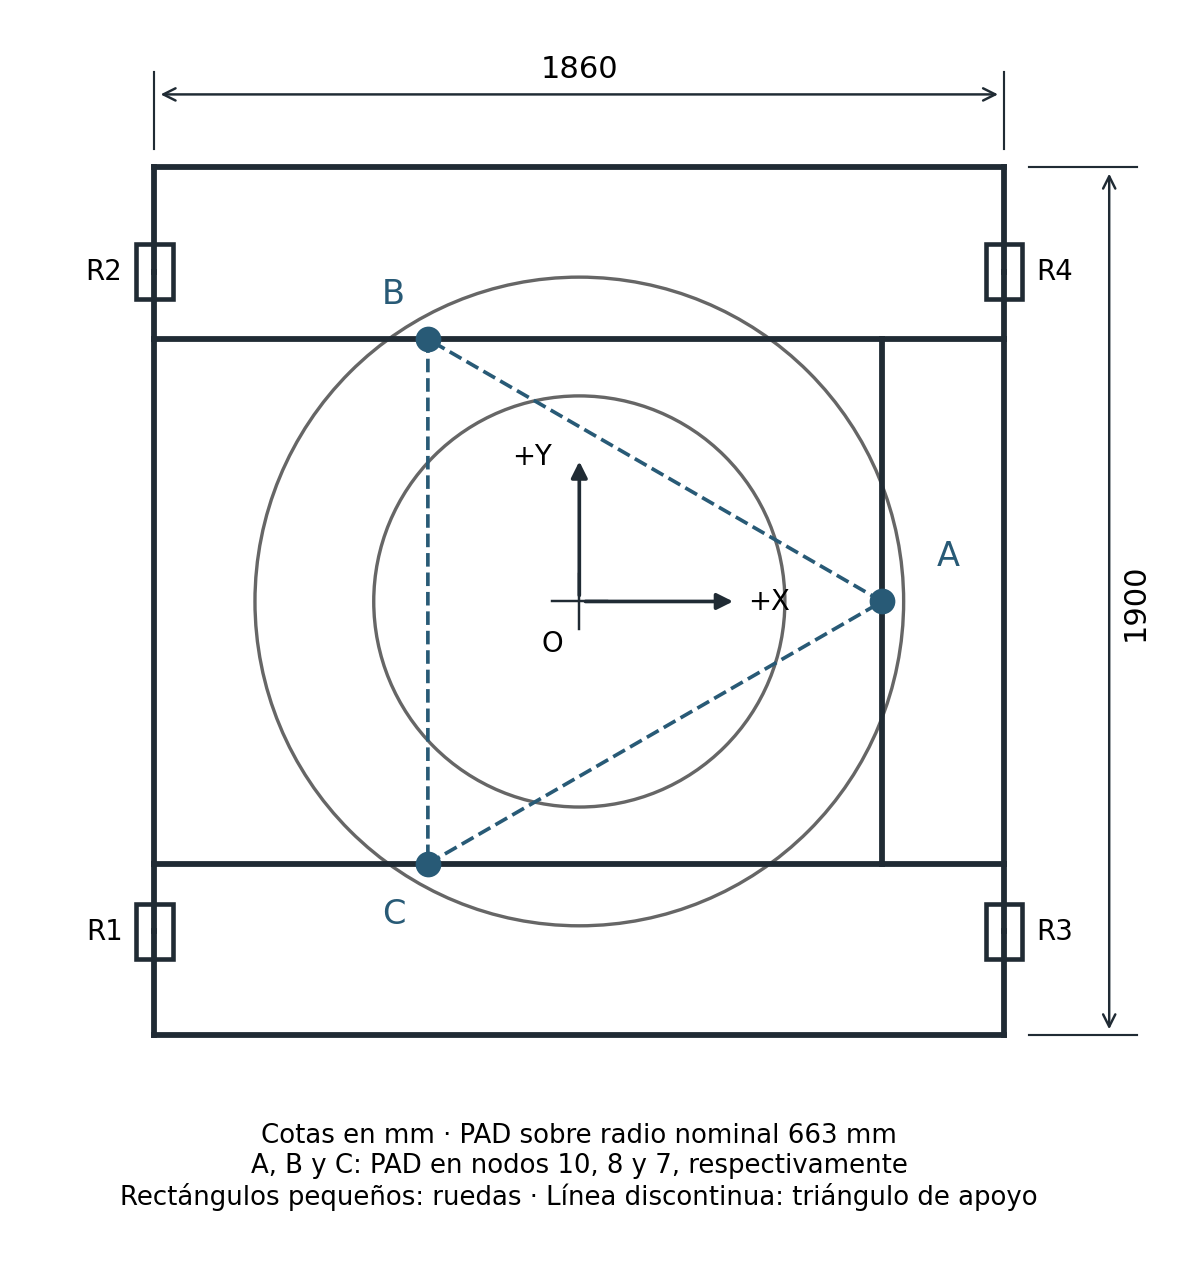
\includegraphics[width=0.92\textwidth]{images/planta_caso_manual}
\caption{Planta de cálculo reconstruida a partir de las coordenadas y la conectividad de la hoja exportada de SAP2000. El rodamiento está centrado; las barras se representan por sus líneas medias. Elaboración propia.}
\label{fig:planta_manual_revision}
\end{figure}

La Tabla~\ref{tab:coordenadas_manual_revision} recoge las coordenadas empleadas en el caso manual.

\begin{table}[htbp]
\centering\small\singlespacing
\caption{Posiciones utilizadas en el cálculo nominal}
\label{tab:coordenadas_manual_revision}
\begin{tabular}{lrrl}
\toprule
\textbf{Elemento} & \textbf{$X$ (mm)} & \textbf{$Y$ (mm)} & \textbf{Nodo SAP}\\
\midrule
Apoyo A & 663,00 & 0,00 & 10\\
Apoyo B & $-331,50$ & 574,18 & 8\\
Apoyo C & $-331,50$ & $-574,18$ & 7\\
Rueda 1 & $-930,00$ & $-722,00$ & 2\\
Rueda 2 & $-930,00$ & 722,00 & 5\\
Rueda 3 & 930,00 & $-722,00$ & 13\\
Rueda 4 & 930,00 & 722,00 & 16\\
\bottomrule
\end{tabular}
\par\smallskip\footnotesize
Fuente: tabla de coordenadas nodales de la exportación original de SAP2000 (Anexo~\ref{anx:programas}). La ordenada 574,18 mm conserva el redondeo de esa exportación; el valor geométrico nominal es aproximadamente 574,175 mm.
\end{table}

\subsubsection{Resolución del equilibrio del rodamiento}

Se aplica el equilibrio de fuerzas y momentos con las reacciones positivas hacia arriba \cite{shigley2015}. Para una resultante vertical que pasa por $(x_r,y_r)$, las ecuaciones son
\begin{equation}
\begin{bmatrix}
1&1&1\\
663&-331{,}5&-331{,}5\\
0&574{,}18&-574{,}18
\end{bmatrix}
\begin{bmatrix}R_A\\R_B\\R_C\end{bmatrix}
=
\begin{bmatrix}W_r\\W_r x_r\\W_r y_r\end{bmatrix}.
\label{eq:manual_matriz_pad}
\end{equation}
La primera fila se expresa en N; las dos restantes, en N\,mm. Para el caso centrado se reemplazan $x_r=y_r=0$ y $W_r=29844$ N:
\begin{align}
R_A+R_B+R_C &=29844,\\
663R_A-331{,}5R_B-331{,}5R_C&=0,\\
574{,}18R_B-574{,}18R_C&=0.
\end{align}
De la tercera ecuación se obtiene $R_B=R_C$. Al sustituir esta relación en la segunda, resulta $663R_A-663R_B=0$ y, por tanto, $R_A=R_B$. Finalmente,
\begin{equation}
\boxed{R_A=R_B=R_C=9948\ \mathrm{N}=9{,}948\ \mathrm{kN}.}
\label{eq:manual_reacciones_pad}
\end{equation}

La suma de las reacciones es 29844 N y sus momentos respecto de los dos ejes se anulan. Sobre el bastidor actúan las fuerzas opuestas, dirigidas hacia abajo. Estas fuerzas coinciden con los tres valores $F_3=-9948$ N registrados en la hoja de cargas nodales. Esa hoja contiene las cargas introducidas en SAP; no es un resultado de una simulación del contacto entre el rodamiento y los apoyos.

Para extender el cálculo a una resultante excéntrica, la resolución de la misma matriz da
\begin{align}
R_A&=\frac{W_r}{3}\left(1+\frac{2x_r}{663}\right),\\
R_B&=\frac{W_r-R_A}{2}+\frac{W_r y_r}{2(574{,}18)},\\
R_C&=\frac{W_r-R_A}{2}-\frac{W_r y_r}{2(574{,}18)}.
\label{eq:manual_pad_general}
\end{align}
Estas expresiones permiten evaluar otras posiciones de la resultante con las mismas coordenadas de apoyo, sin repetir su desarrollo algebraico.

\subsubsection{Contacto compresivo y presión media}

En una interfaz sin amarre vertical se exige reacción normal no negativa. Si $g_i$ representa la separación entre superficies, las condiciones ideales son
\begin{equation}
R_i\geq0,\qquad g_i\geq0,\qquad R_i g_i=0.
\label{eq:manual_contacto}
\end{equation}
Para el caso centrado se adopta la hipótesis de tres apoyos asentados, $g_A=g_B=g_C=0$. Las tres reacciones calculadas son positivas, de modo que la hipótesis es estáticamente admisible. Esta comprobación corresponde a apoyos puntuales ideales; no determina la distribución real de presión en un revestimiento deformable.

El área geométrica de cada liner, representado por un sector entre radios de 638 y 688 mm y ángulo de $24^\circ$, resulta
\begin{equation}
A=\frac{24\pi}{360}\left(688^2-638^2\right)
=13885{,}840\ \mathrm{mm^2}.
\label{eq:manual_area}
\end{equation}
Si toda esa área participa en el contacto, la presión media del caso nominal es
\begin{equation}
\boxed{p_m=\frac{9948}{13885{,}840}=0{,}7164\ \mathrm{MPa}.}
\label{eq:manual_presion}
\end{equation}
El resultado establece una demanda media de referencia. Para comprobar el liner se necesita el área efectiva y la resistencia admisible correspondiente a su material, temperatura y duración de la carga. Si la huella efectiva disminuye, la presión media aumenta.

La factibilidad se evalúa antes de aceptar una reacción máxima. Como comprobación del procedimiento, una resultante situada en $x_r=-400$ mm y $y_r=0$ produce
\[
R_A=-2055{,}620\ \mathrm{N},\qquad
R_B=R_C=15949{,}810\ \mathrm{N}.
\]
La reacción negativa indica que esa terna no puede sostener la carga con contactos exclusivamente compresivos y se rechaza esa solución. No se sustituye el valor negativo por cero, porque así se perdería el equilibrio de momentos. Este ejemplo es una prueba matemática fuera del triángulo de apoyo, no una posición de trabajo del rodamiento (Figura~\ref{fig:contacto_manual_revision}).

En el caso nominal, la resultante permanece dentro del triángulo y las tres reacciones son compresivas. La tolerancia propuesta de colocación de 5 mm requiere además revisar la cobertura del aro sobre cada apoyo. El triángulo de apoyo y la huella real del liner representan comprobaciones geométricas diferentes.

\begin{figure}[htbp]
\centering
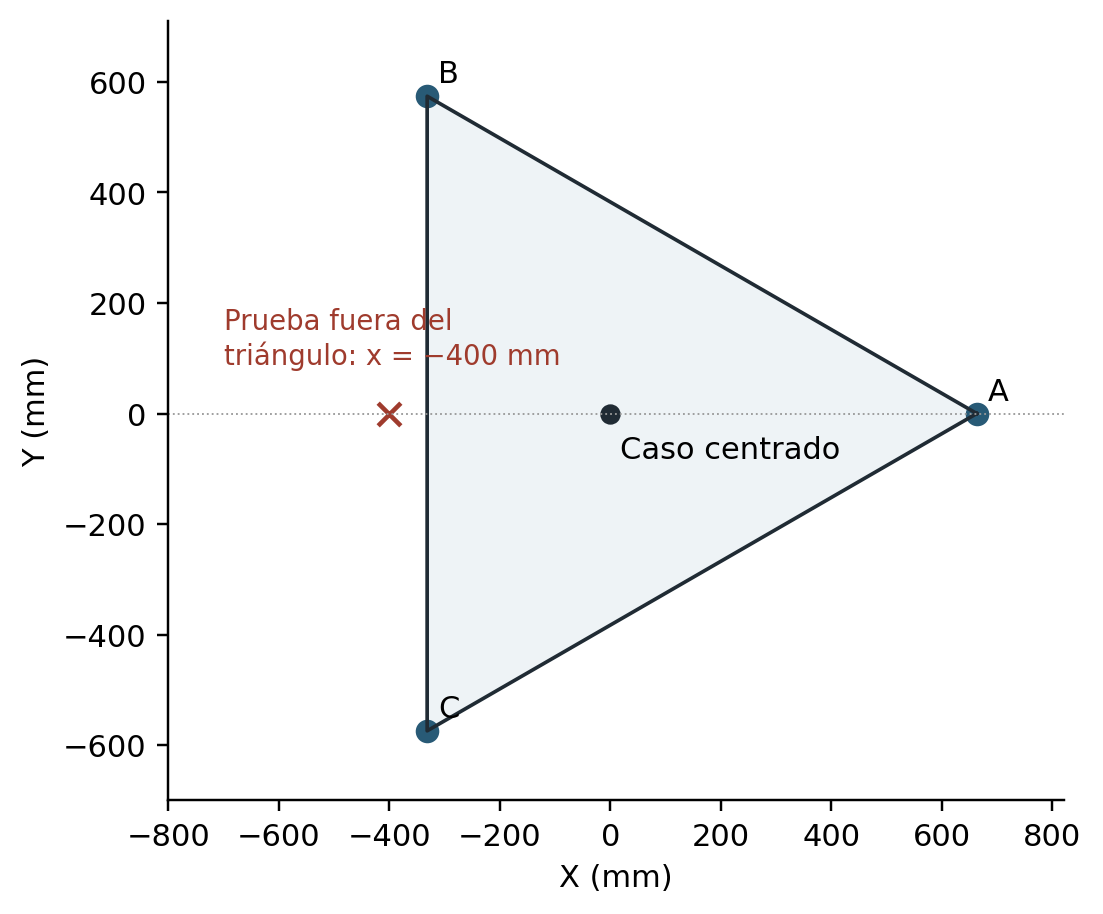
\includegraphics[width=0.84\textwidth]{images/factibilidad_pad}
\caption{Posición de la resultante del caso centrado y de la prueba matemática fuera del triángulo de apoyo. Elaboración propia a partir de las coordenadas del modelo.}
\label{fig:contacto_manual_revision}
\end{figure}

La Figura~\ref{fig:contacto_manual_revision} muestra ambas posiciones. El ejemplo exterior corresponde a una solución inadmisible porque exigiría tracción en un apoyo.

\subsubsection{Equilibrio del bastidor y reacciones en las ruedas}

La carga externa está centrada, pero la distribución de perfiles no es simétrica respecto de $X=0$: existe un miembro adicional en el lado del apoyo A. Para obtener el centro del peso propio se utilizan las longitudes y centroides de los 20 elementos de barra. Como todos tienen la misma sección y se adopta peso por unidad de longitud uniforme, el centro se calcula mediante
\begin{equation}
x_b=\frac{\sum_j L_j x_j}{\sum_j L_j},\qquad
y_b=\frac{\sum_j L_j y_j}{\sum_j L_j}.
\label{eq:manual_cg_perfiles}
\end{equation}
Con los valores de la tabla de conectividad de barras, se obtiene
\[
\sum_jL_j=12388{,}38\ \mathrm{mm},\quad
x_b=61{,}457808\ \mathrm{mm},\quad y_b\simeq0.
\]
El peso propio de barras se toma como una entrada del caso de referencia, $W_b=1648{,}74$ N. Su distribución se calcula a partir de la geometría, sin utilizar las reacciones individuales de SAP. El peso total y su primer momento respecto del plano $X=0$ son
\begin{align}
W_t&=29844+1648{,}74=31492{,}74\ \mathrm{N},\\
W_bx_b&=1648{,}74(61{,}457808)
=101327{,}946\ \mathrm{N\,mm}.
\label{eq:manual_peso_momento}
\end{align}

La geometría, las cargas y el campo vertical de la solución se consideran simétricos respecto de $Y=0$. En la idealización lineal de este caso, se conserva así la igualdad de las dos reacciones de cada lado: $R_1=R_2$ y $R_3=R_4$. Para evitar extender esta simplificación a otros escenarios, se limita a la carga vertical centrada y a los apoyos del modelo de referencia.

Al definir $R_-=R_1+R_2$ y $R_+=R_3+R_4$, el equilibrio exige
\begin{align}
R_-+R_+&=W_t,\\
930(R_+-R_-)&=W_bx_b.
\end{align}
Las reacciones individuales quedan
\begin{align}
R_1=R_2&=\frac{1}{4}\left(W_t-\frac{W_bx_b}{930}\right)
 =7845{,}9463\ \mathrm{N},\\
R_3=R_4&=\frac{1}{4}\left(W_t+\frac{W_bx_b}{930}\right)
 =7900{,}4237\ \mathrm{N}.
\label{eq:manual_ruedas}
\end{align}

La diferencia de carga entre ambos lados responde al centro del peso de los perfiles. El centro del rodamiento continúa en $(0,0)$. Tampoco debe confundirse este centro del bastidor analítico con el centro de gravedad del conjunto móvil, que incluye ruedas, mecanismos y otros accesorios. La Tabla~\ref{tab:manual_sap_revision} contrasta estas reacciones con las de la exportación de SAP2000.

\begin{table}[htbp]
\centering\small\singlespacing
\caption{Comparación de reacciones verticales del caso nominal}
\label{tab:manual_sap_revision}
\begin{tabular}{lrrr}
\toprule
\textbf{Nodo} & \textbf{Manual (N)} & \textbf{SAP (N)} & \textbf{Manual $-$ SAP (N)}\\
\midrule
2 & 7845,9463 & 7845,95 & $-0,0037$\\
5 & 7845,9463 & 7845,95 & $-0,0037$\\
13 & 7900,4237 & 7900,42 & 0,0037\\
16 & 7900,4237 & 7900,42 & 0,0037\\
\midrule
Total & 31492,7400 & 31492,74 & 0,0000\\
\bottomrule
\end{tabular}
\par\smallskip\footnotesize
Fuente: tabla de reacciones nodales de la exportación original de SAP2000, combinación nominal. El cálculo manual utiliza el peso propio total exportado y distribuye ese peso mediante la geometría de barras.
\end{table}

Las diferencias individuales son inferiores a 0,004 N, compatibles con la precisión de las tablas exportadas. El mayor error relativo es aproximadamente \SI{0.0000471}{\percent}. La comprobación confirma la suma y la distribución de reacciones del caso vertical centrado. No es una verificación independiente de la rigidez, del índice resistente ni de los contactos en situaciones de desnivel.

Las cuatro reacciones nominales son positivas. Este resultado es compatible con cuatro contactos cerrados en ese caso, pero los apoyos verticales del modelo SAP son bilaterales. La ausencia de levantamiento en otros escenarios requiere resolver las separaciones y reacciones de cada contacto; no se deduce de una sola combinación favorable.

\subsubsection{Cálculo manual de la flecha relativa a partir de SAP}

Se utiliza el travesaño comprendido entre los nodos 3 y 14, cuya luz es $L=1860$ mm. El nodo 7 está a $598{,}5$ mm del nodo 3. Para la combinación nominal, la exportación registra
\[
u_3=-0{,}117051\ \mathrm{mm},\quad
u_{14}=-0{,}117920\ \mathrm{mm},\quad
u_7=-1{,}353133\ \mathrm{mm}.
\]
La cuerda que une los extremos deformados tiene, en el nodo 7, el desplazamiento
\begin{align}
u_c&=u_3+\frac{598{,}5}{1860}(u_{14}-u_3)\\
&=-0{,}117330622\ \mathrm{mm}.
\end{align}
La flecha relativa absoluta es
\begin{equation}
\boxed{|\delta_{\mathrm{rel},7}|=|u_7-u_c|
=1{,}235802378\ \mathrm{mm}.}
\label{eq:manual_flecha}
\end{equation}
Para el criterio de proyecto propuesto,
\[
\frac{L}{800}=2{,}325\ \mathrm{mm},\qquad
\frac{|\delta_{\mathrm{rel},7}|}{L/800}=0{,}53153.
\]
El nodo evaluado queda por debajo de ese límite. La búsqueda del máximo a lo largo del miembro se realiza con las estaciones del modelo. El valor global $|U_3|$ no se reemplaza ni se confunde con la flecha relativa.

Este desarrollo muestra cómo se procesa un resultado de SAP. Una predicción manual independiente de desplazamiento requiere las inercias efectivas, las condiciones de unión y el modelo de cargas del elemento elegido, además del módulo elástico indicado en el apartado~\ref{sec:material-trazabilidad}. La interpolación de los desplazamientos exportados comprueba únicamente el posproceso.

\subsubsection{Extensión a los demás casos}

Las ecuaciones anteriores permiten extender el caso centrado a otras posiciones de la resultante y áreas de contacto. No se dispone de una hoja complementaria que reúna estas operaciones para los tres modelos de bastidor; el contraste se sustenta en el desarrollo explícito y las tablas originales, como se precisa en el apartado~\ref{sec:respaldo-complementario}. La comparación entre tres, cuatro y cinco apoyos emplea la misma carga externa total, con el reparto impuesto que se utilizó en los modelos disponibles:
\begin{equation}
P_{\mathrm{ap}}=\frac{W_r}{n}
\quad\Rightarrow\quad
9948;\ 7461;\ 5968{,}8\ \mathrm{N}
\quad\text{para } n=3,\ 4,\ 5.
\label{eq:manual_reparto_comparativo}
\end{equation}
Para tres apoyos no colineales, la carga centrada y el equilibrio justifican el reparto calculado. Para cuatro o cinco apoyos, el equilibrio vertical y los dos momentos no bastan para determinar todas las reacciones. Los valores iguales se conservan como cargas impuestas para comparar el bastidor; el contacto real requiere incorporar rigideces y compatibilidad de deformaciones.

Los desplazamientos y los índices resistentes se mantienen como resultados de las corridas originales. Modificar una masa en un cálculo analítico no actualiza esos resultados ni sustituye la solución del modelo estructural.

\section{Dimensionamiento analítico del sistema de aspersión}
\label{sec:man-asp-base}

El sistema de aspersión debe suministrar líquido a las superficies exteriores
y al agujero del rodamiento mientras la pieza permanece inmóvil sobre sus
tres apoyos. El distribuidor gira alrededor del eje vertical de la pieza y
alimenta dos ramales exteriores, un ramal interior y dos grupos superiores.
El dimensionamiento determina cuántas boquillas se requieren, cuánto
líquido debe circular, qué presión debe proporcionar la bomba y qué potencia
demanda el bombeo. La cobertura geométrica se evalúa por separado, porque
disponer de presión y caudal no demuestra por sí solo la remoción de grasa.

Se aplican la conservación de masa, el balance de energía de Bernoulli,
las pérdidas de Darcy--Weisbach y el balance de cantidad de movimiento.
Estas relaciones se desarrollan a continuación con los datos, las
sustituciones numéricas y la interpretación de cada resultado.

\subsection{Datos de diseño y supuestos de cálculo}
\label{sec:man-asp-datos}

El rodamiento de referencia es el SKF 241/900 ECAK30/W33. Sus diámetros
exterior e interior son 1420 y 900 mm, y su ancho axial es 515 mm
\cite{skf241}. En posición de lavado, el eje del rodamiento es vertical.
Las cotas $z$ de este desarrollo se miden desde el piso de la cabina; por
consiguiente, no se confunden con la distancia medida desde el centro de
la pieza. Se adoptan $z_{inf}=890$ mm y $z_{sup}=1405$ mm para sus caras. La
Tabla~\ref{tab:man-asp-base} reúne las condiciones geométricas y operativas del caso.

\begin{table}[htbp]
\centering\small
\caption{Condiciones geométricas y operativas del caso base.}
\label{tab:man-asp-base}
\begin{tabularx}{\linewidth}{@{}>{\raggedright\arraybackslash}X l >{\raggedright\arraybackslash}p{4.1cm}@{}}
\toprule Parámetro & Valor & Condición\\\midrule
Diámetro exterior $D$ & 1420 mm & Dato del rodamiento.\\
Diámetro interior menor $d$ & 900 mm & Agujero cónico 1:30.\\
Ancho axial $B$ & 515 mm & Dato del rodamiento.\\
Temperatura nominal $T$ & 62 $^\circ$C & Condición de diseño adoptada.\\
Presión mínima de boquilla $p_n$ & 4 bar & Presión manométrica propuesta.\\
Distancia lateral $s_e$ & 125,85 mm & Separación geométrica adoptada.\\
Distancia interior $s_i$ & 143,30 mm & Separación geométrica adoptada.\\
Distancia superior $s_s$ & 184,85 mm & Separación geométrica adoptada.\\
Ángulo de abanico $\theta$ & 50$^\circ$ & Ángulo de cálculo adoptado.\\
Solape mínimo objetivo $\phi$ & 25\,\% & Criterio geométrico propuesto.\\
\bottomrule
\end{tabularx}
\end{table}

Se supone régimen permanente, líquido incompresible y tuberías llenas.
El detergente diluido se aproxima inicialmente mediante las propiedades
del agua a 62 $^\circ$C. Esta simplificación permite predimensionar la red;
deberá revisarse al conocer la formulación y concentración del producto.
Las propiedades se obtuvieron de la biblioteca CoolProp, que implementa
las formulaciones de referencia para el agua \cite{bell2014}:
\begin{equation}
 \rho=982{,}120\ \mathrm{kg/m^3},\qquad
 \mu=4{,}52269\times10^{-4}\ \mathrm{Pa\,s},\qquad
 p_v=21866{,}997\ \mathrm{Pa}.
 \label{eq:man-asp-props}
\end{equation}
La viscosidad cinemática se obtiene dividiendo la viscosidad dinámica por
la densidad:
\begin{equation}
 \nu=\frac{\mu}{\rho}
 =\frac{4{,}52269\times10^{-4}\ \mathrm{kg/(m\,s)}}
 {982{,}120\ \mathrm{kg/m^3}}
 =4{,}60503\times10^{-7}\ \mathrm{m^2/s}.
 \label{eq:man-asp-nu}
\end{equation}
Se utiliza $g=9{,}81$ m/s$^2$. En la hidráulica, $Q$ representa el caudal
de una tubería y $q$ el caudal de una boquilla. Los cálculos de pérdidas
se efectúan en metros, segundos y pascales; en la geometría de huellas
se mantienen milímetros. Un bar equivale a $10^5$ Pa y un L/min a
$1/60000$ m$^3$/s.

\subsection{Caudal y velocidad de una boquilla}
\label{sec:man-asp-boquilla}

Se toma como referencia hidráulica una boquilla de abanico plano H3/8U-5020,
cuya ficha indica 2 gal/min estadounidenses a 40 psi y un diámetro equivalente
de 0,109 pulgadas \cite{manSpray}. Se emplea su capacidad para el cálculo,
sin considerar cerrado el material comercial de la boquilla ni su
compatibilidad con la solución de limpieza.

\subsubsection{Conversión del punto nominal}
El caudal y la presión de catálogo se convierten antes de aplicar las ecuaciones:
\begin{align}
 q_r&=2\ \frac{\mathrm{gal}}{\mathrm{min}}
 \left(3{,}785411784\ \frac{\mathrm{L}}{\mathrm{gal}}\right)
 =7{,}57082\ \mathrm{L/min},\label{eq:man-asp-qr}\\
 p_r&=40\ \mathrm{psi}\left(6894{,}757\ \frac{\mathrm{Pa}}{\mathrm{psi}}\right)
 =275790{,}28\ \mathrm{Pa}=2{,}75790\ \mathrm{bar}.
 \label{eq:man-asp-pr}
\end{align}

\subsubsection{Caudal a la presión de diseño}
Para el mismo orificio y propiedades aproximadamente constantes,
$q$ varía con la raíz cuadrada de la presión diferencial. Así,
\begin{equation}
 q=q_r\sqrt{\frac{p_n}{p_r}}
 =7{,}57082\sqrt{\frac{4{,}00000}{2{,}75790}}
 =\boxed{9{,}11767\ \mathrm{L/min}}.
 \label{eq:man-asp-q}
\end{equation}
La presión de la Ecuación~\eqref{eq:man-asp-q} es la diferencia entre la
entrada de la boquilla y la cabina, considerada a presión atmosférica.
No es la presión absoluta del líquido. La misma relación puede escribirse
como $q=K_q\sqrt{p_n}$, con
\begin{equation}
 K_q=\frac{7{,}57082}{\sqrt{2{,}75790}}
 =4{,}55883\ \frac{\mathrm{L}}{\mathrm{min}\sqrt{\mathrm{bar}}}.
 \label{eq:man-asp-kq}
\end{equation}
Este coeficiente se utiliza después para actualizar el caudal de cada
boquilla cuando su presión difiere ligeramente de 4 bar. Se conserva el
coeficiente nominal de catálogo; la variación por temperatura y detergente
debe comprobarse con el fabricante.

\subsubsection{Velocidad y escala de fuerza del chorro}
Se adopta un coeficiente de velocidad $C_v=0{,}95$ como hipótesis. La
velocidad característica estimada es
\begin{equation}
 v_j=C_v\sqrt{\frac{2p_n}{\rho}}
 =0{,}95\sqrt{\frac{2(400000)}{982{,}120}}
 =\boxed{27{,}114\ \mathrm{m/s}}.
 \label{eq:man-asp-vj}
\end{equation}
Primero se convierte el caudal a SI:
\begin{equation}
 q=\frac{9{,}11767}{60000}=1{,}51961\times10^{-4}\ \mathrm{m^3/s}.
\end{equation}
El flujo de cantidad de movimiento proporciona una escala de fuerza:
\begin{equation}
 F\simeq\rho qv_j
 =(982{,}120)(1{,}51961\times10^{-4})(27{,}114)
 =\boxed{4{,}047\ \mathrm{N}}.
 \label{eq:man-asp-f}
\end{equation}
Esta fuerza corresponde a una representación equivalente del chorro. No
es una medición de impacto sobre la grasa ni un valor de esfuerzo cortante
de pared; ambos dependen de la distribución real del abanico y de la distancia.

Como comprobación dimensional del orificio,
$d_{eq}=0{,}109(25{,}4)=2{,}7686$ mm y
$A_{eq}=\pi(0{,}0027686)^2/4=6{,}02019\times10^{-6}$ m$^2$.
El coeficiente de descarga implícito resulta
\begin{equation}
 C_d=\frac{q}{A_{eq}\sqrt{2p_n/\rho}}
 =\frac{1{,}51961\times10^{-4}}
 {(6{,}02019\times10^{-6})(28{,}5406)}
 \simeq0{,}884.
 \label{eq:man-asp-cd}
\end{equation}
El área es equivalente: no representa necesariamente un orificio circular
real ni permite reemplazar el abanico por un chorro cilíndrico en una
simulación sin justificar esa idealización.

\subsection{Número de boquillas y cobertura nominal}
\label{sec:man-asp-cobertura}

Una boquilla de abanico plano situada a distancia $s$, con incidencia normal,
produce una anchura geométrica
\begin{equation}
 b=2s\tan(\theta/2).
 \label{eq:man-asp-b}
\end{equation}
La ecuación se obtiene de los dos triángulos rectángulos formados por el eje
del chorro y sus rayos extremos. Describe la envolvente ideal del abanico,
no una distribución uniforme de caudal sobre toda la huella.

Si dos huellas de ancho $b$ deben superponerse una fracción $\phi$, la
separación máxima entre centros es $a_{max}=b(1-\phi)$. Con $N$ boquillas,
la longitud cubierta es $b+(N-1)a_{max}$. Para cubrir una longitud $L$ se exige
\begin{equation}
 b+(N-1)b(1-\phi)\geq L
 \quad\Longrightarrow\quad
 N\geq1+\frac{L-b}{b(1-\phi)}.
 \label{eq:man-asp-n}
\end{equation}
Se redondea hacia arriba porque la cantidad de boquillas debe ser entera,
con un mínimo de una.

\subsubsection{Ramal interior}
La longitud objetivo es el ancho axial del rodamiento, $L=515$ mm:
\begin{align}
 b_i&=2(143{,}30)\tan25^\circ=133{,}644\ \mathrm{mm},\\
 N_i&\geq1+\frac{515-133{,}644}{133{,}644(1-0{,}25)}
 =4{,}805\quad\Longrightarrow\quad\boxed{N_i=5}.
\end{align}
Una vez fijado $N_i$, se distribuyen sus centros uniformemente:
\begin{align}
 a_i&=\frac{515-133{,}644}{5-1}=95{,}339\ \mathrm{mm},\\
 \phi_i&=1-\frac{95{,}339}{133{,}644}=0{,}2866.
\end{align}
El solape nominal es 28,66\,\%, superior al 25\,\% propuesto.
La primera boquilla queda a $890+b_i/2=956{,}822$ mm y las siguientes
a esa cota más múltiplos de $a_i$. Así se obtienen, redondeando a décimas,
$z=956{,}8;1052{,}2;1147{,}5;1242{,}8;1338{,}2$ mm.

\subsubsection{Grupos superiores}
La anchura radial de la cara anular es
$L_s=(1420-900)/2=260$ mm. Por cada lado del distribuidor:
\begin{align}
 b_s&=2(184{,}85)\tan25^\circ=172{,}394\ \mathrm{mm},\\
 N_s&\geq1+\frac{260-172{,}394}{172{,}394(0{,}75)}
 =1{,}678\quad\Longrightarrow\quad\boxed{N_s=2},\\
 a_s&=\frac{260-172{,}394}{2-1}=87{,}606\ \mathrm{mm}.
\end{align}
Sus radios nominales son $450+b_s/2=536{,}197$ mm y
$536{,}197+87{,}606=623{,}803$ mm. Se requieren cuatro boquillas
superiores en total. El solape radial nominal es 49,18\,\%.
La cobertura sobre la proyección anular no demuestra el alcance de las
superficies internas entre aros, rodillos y jaula.

\subsubsection{Ramales exteriores}
Se obtiene $b_e=2(125{,}85)\tan25^\circ=117{,}370$ mm.
El caso base dispone cuatro boquillas de eje radial por ramal, con centros
entre 1100 mm y $1405-b_e/2=1346{,}315$ mm. Su separación es
\begin{equation}
 a_e=\frac{1346{,}315-1100}{4-1}=82{,}105\ \mathrm{mm},\qquad
 \phi_e=1-\frac{82{,}105}{117{,}370}=0{,}3005.
\end{equation}
Estas cuatro boquillas cubren nominalmente desde
$1100-117{,}370/2=1041{,}315$ mm hasta 1405 mm. El solape de
30,05\,\% se refiere únicamente a ellas. Para intentar alcanzar la zona
inferior se propone una quinta boquilla inclinada en cada ramal.

\subsubsection{Comprobación de la boquilla inclinada}
Su centro está a $z_n=1070$ mm y su eje apunta hacia $z_t=950$ mm.
La inclinación descendente es
\begin{equation}
 \alpha=\arctan\left(\frac{1070-950}{125{,}85}\right)=43{,}637^\circ.
\end{equation}
En un plano radial vertical, cada rayo recorre horizontalmente $s_e$ hasta
la generatriz del rodamiento. Sus descensos son $s_e\tan(\alpha\pm25^\circ)$;
por tanto, los bordes no son simétricos respecto del punto de impacto del eje:
\begin{align}
 z_{min}&=1070-125{,}85\tan(43{,}637^\circ+25^\circ)
 =748{,}259\ \mathrm{mm},\\
 z_{max}&=1070-125{,}85\tan(43{,}637^\circ-25^\circ)
 =1027{,}557\ \mathrm{mm}.
 \label{eq:man-asp-inclinada}
\end{align}
La intersección de esta huella ideal con la superficie exterior existente
comienza a 890 mm. Entre su borde superior y la huella radial siguiente queda
\begin{equation}
 \Delta z_{sin\ cobertura}=1041{,}315-1027{,}557
 =\boxed{13{,}759\ \mathrm{mm}}.
 \label{eq:man-asp-hueco}
\end{equation}
En consecuencia, la distribución lateral propuesta no garantiza cobertura
axial completa en esta posición nominal. Debe ajustarse la orientación o la
ubicación de la boquilla y comprobarse el barrido con oscilación y las sombras
del soporte. El cálculo hidráulico posterior corresponde a esta configuración
base de 19 boquillas, cuya distribución detalla la
Tabla~\ref{tab:man-asp-cantidad}; no implica que el problema de cobertura esté resuelto.

\begin{table}[htbp]
\centering\small
\caption{Cantidad de boquillas del caso base hidráulico.}
\label{tab:man-asp-cantidad}
\begin{tabularx}{\linewidth}{@{}Xrr@{}}
\toprule Grupo & Distribución & Total\\\midrule
Ramales exteriores & $2(4+1)$ & 10\\
Ramal interior & $1(5)$ & 5\\
Grupos superiores & $2(2)$ & 4\\\midrule
Total simultáneo & & 19\\\bottomrule
\end{tabularx}
\end{table}

\subsection{Primera estimación del caudal total}
\label{sec:man-asp-qtotal}
Si todas las boquillas reciben exactamente 4 bar, el caudal es
\begin{equation}
 Q_0=Nq=19(9{,}11767)
 =173{,}236\ \mathrm{L/min}
 =2{,}88726\times10^{-3}\ \mathrm{m^3/s}.
 \label{eq:man-asp-q0}
\end{equation}
Esta es una primera estimación por continuidad, no un caudal asignado a
cada tubo del distribuidor. Cada tramo transporta la suma de las boquillas
que tiene aguas abajo. La diferencia de elevación y las pérdidas generan
presiones ligeramente distintas; la sección siguiente determina esa
corrección y el caudal que se empleará en la alimentación principal.
\subsection{Modelo hidráulico y cálculo de la distribución}
\label{sec:man-asp-red}

Se identifica como $C$ la salida de alimentación central, situada a
$z_C=1{,}770$ m. Desde ella parten dos recorridos exteriores simétricos
y un recorrido interior. En cada lado exterior, $S1$ y $S2$ son las tomas
superiores; $E0$ es el inicio del tubo descendente y $E1$ a $E5$ son sus
tomas. En el ramal interior, $I0$ es la entrada y $I1$ a $I5$ son las
tomas ordenadas de arriba hacia abajo. Los puntos de la
Figura~\ref{fig:man-asp-esquema} son estaciones de cálculo, no un plano
de montaje.

\begin{figure}[htbp]
\centering
\begin{tikzpicture}[>=Stealth, every node/.style={font=\small},
 box/.style={draw,rounded corners=2pt,align=center,minimum height=10mm,text width=24mm},
 flow/.style={->,thick}]
\node[box] (tan) at (0,0) {Depósito\\abierto};
\node[box] (bom) at (3.3,0) {Bomba};
\node[box] (fil) at (6.6,0) {Filtro};
\node[box] (uni) at (9.9,0) {Unión\\rotativa};
\draw[flow] (tan)--node[above,font=\scriptsize]{DN50}(bom);
\draw[flow] (bom)--node[above,font=\scriptsize]{DN40}(fil);
\draw[flow] (fil)--node[above,font=\scriptsize]{DN40}(uni);
\node[box] (c) at (9.9,-1.8) {$C$\\Distribución};
\draw[flow] (uni)--node[right,font=\scriptsize]{DN40}(c);
\node[box,text width=34mm] (a) at (0,-3.6) {Lado exterior 1\\$S1,S2,E1\ldots E5$\\7 boquillas};
\node[box,text width=34mm] (b) at (4.9,-3.6) {Lado exterior 2\\Simétrico al lado 1\\7 boquillas};
\node[box,text width=34mm] (i) at (9.9,-3.6) {Ramal interior\\$I1\ldots I5$\\5 boquillas};
\draw[flow] (c.west)--(0,-1.8)--(a.north);
\draw[flow] (4.9,-1.8)--(b.north);
\draw[flow] (c)--(i);
\node[align=center,text width=12cm] at (4.9,-5) {Después de la aplicación, el líquido retorna al depósito.\\El dimensionamiento del retorno y del tanque se evalúa por separado.};
\end{tikzpicture}
\caption{Esquema funcional del circuito y de los grupos simultáneos. Elaboración propia; sin escala.}
\label{fig:man-asp-esquema}
\end{figure}

\subsubsection{Geometría hidráulica adoptada}
Se consideran diámetros exteriores de 33,4; 48,3 y 60,3 mm, con espesor
de 2,77 mm. El diámetro que interviene en la velocidad es el interior:
\begin{equation}
 D_{25}=33{,}4-2(2{,}77)=27{,}86\ \mathrm{mm},\quad
 D_{40}=42{,}76\ \mathrm{mm},\quad D_{50}=54{,}76\ \mathrm{mm}.
\end{equation}
Estas dimensiones se adoptan para el predimensionamiento y deben cotejarse
con la tubería suministrada. Se supone rugosidad $\varepsilon=0{,}045$ mm.

\subsubsection{Ecuaciones por tramo}
Para cada tubo se calculan la velocidad, Reynolds y factor de Darcy:
\begin{align}
 v&=\frac{4Q}{\pi D_i^2},\qquad Re=\frac{\rho vD_i}{\mu},
 \label{eq:man-asp-vre}\\
 f&=\frac{0{,}25}{\left[\log_{10}\left(
 \frac{\varepsilon}{3{,}7D_i}+\frac{5{,}74}{Re^{0{,}9}}\right)\right]^2}.
 \label{eq:man-asp-sj}
\end{align}
La Ecuación~\eqref{eq:man-asp-sj} es la aproximación de Swamee--Jain para
el régimen turbulento \cite{manSwamee}. Las pérdidas del tramo son
\begin{equation}
 h_L=h_f+h_m
 =\left(f\frac{L}{D_i}+\sum K_m\right)\frac{v^2}{2g}.
 \label{eq:man-asp-hl}
\end{equation}
Los coeficientes $K_m$ son adimensionales y se refieren a la velocidad del
tramo donde se colocan. No deben confundirse con el coeficiente de boquilla
$K_q$. Para el caso base se adoptan factores $f_T$ de 0,023; 0,020 y 0,019
para DN25, DN40 y DN50; se representan un paso de derivación por $20f_T$,
una salida de derivación por $60f_T$ y un codo por $30f_T$.
Son coeficientes de predimensionamiento, sujetos a confirmación con los
accesorios reales. Por ejemplo, la entrada a un lado exterior toma
$60(0{,}019)=1{,}14$, y la entrada interior,
$(60+30)(0{,}023)=2{,}07$.

\subsubsection{Relación entre presión, caudal y elevación}
En un tramo sin bomba, Bernoulli proporciona
\begin{equation}
 \frac{p_j}{\rho g}+z_j+\frac{v_j^2}{2g}
 =\frac{p_i}{\rho g}+z_i+\frac{v_i^2}{2g}-h_{L,ij}.
 \label{eq:man-asp-bernoulli-ramal}
\end{equation}
Para la primera aproximación de los colectores se desprecia la diferencia
de cargas cinéticas entre sus estaciones. Así,
\begin{equation}
 p_j\simeq p_i-\rho g\left[h_{L,ij}+(z_j-z_i)\right],\qquad
 q_j=K_q\sqrt{p_j},
 \label{eq:man-asp-recursion}
\end{equation}
con $p_j$ en bar únicamente en la segunda expresión, por las unidades
elegidas para $K_q$. La primera expresión emplea pascales.
La menor elevación incrementa la presión; la pérdida de carga la reduce.
Las tomas superiores se representan a 1,740 m, en el colector. El descenso
dentro del cuerpo y de las conexiones de cada boquilla no se modela.
Las diferencias cinéticas y estas conexiones se deben incluir al cerrar
la red; por ello se presenta un predimensionamiento, no una predicción
exacta de la instalación.

\subsubsection{Procedimiento de solución por aproximaciones sucesivas}
Se inicia con $q_j=9{,}11767$ L/min y $p_C=4$ bar. Se suman los caudales
aguas abajo de cada tramo, se calculan sus pérdidas y se obtienen las
presiones con la Ecuación~\eqref{eq:man-asp-recursion}. Después se actualiza
cada caudal con su presión y se ajusta la presión central mediante
\begin{equation}
 p_C^{(k+1)}=p_C^{(k)}+\left(4-p_{min}^{(k)}\right)
 \quad[\mathrm{bar}].
 \label{eq:man-asp-iteracion}
\end{equation}
Así se busca que la toma más desfavorable tenga 4 bar. Es una resolución
de ecuaciones de continuidad y energía; las sucesivas aproximaciones se
exponen para que el cálculo pueda comprobarse con una calculadora: la
Tabla~\ref{tab:man-asp-iteraciones} registra las aproximaciones y la
Tabla~\ref{tab:man-asp-tramos}, los tramos del estado convergido.

\begin{table}[htbp]
\centering\small
\caption{Aproximaciones sucesivas para determinar la presión central.}
\label{tab:man-asp-iteraciones}
\input{aspersion_manual/tabla_iteraciones}
\end{table}
En las dos últimas filas la diferencia de caudal total es menor que
0,001 L/min. Los dígitos adicionales permiten revisar el cierre aritmético;
no representan la precisión física de las hipótesis.

\begin{table}[htbp]
\centering\small
\caption{Datos por tramo y pérdidas del estado convergido.}
\label{tab:man-asp-tramos}
\input{aspersion_manual/tabla_tramos}
\par\smallskip\footnotesize
Se muestra un lado exterior; el segundo es simétrico. $z_f$ es la elevación
final del tramo. Los caudales y pérdidas son resultados; $L$, DN y
$\sum K_m$ son entradas del modelo.
\end{table}

\subsubsection{Ejemplo completo: primer tramo del lado exterior}
El tramo $C$--$S1$ alimenta siete boquillas. En el estado convergido conduce
$Q=64{,}11274$ L/min $=1{,}06855\times10^{-3}$ m$^3$/s. Se tiene
$D_i=0{,}05476$ m, $L=0{,}536$ m y $\sum K_m=1{,}14$. Entonces:
\begin{align}
 v&=\frac{4(1{,}06855\times10^{-3})}{\pi(0{,}05476)^2}
 =0{,}45371\ \mathrm{m/s},\\
 Re&=\frac{982{,}120(0{,}45371)(0{,}05476)}{4{,}52269\times10^{-4}}
 =5{,}3952\times10^4,\\
 f&=\frac{0{,}25}{\left[\log_{10}\left(
 \frac{0{,}000045}{3{,}7(0{,}05476)}+
 \frac{5{,}74}{(53952)^{0{,}9}}\right)\right]^2}=0{,}023396,\\
 h_{L,C-S1}&=\left(0{,}023396\frac{0{,}536}{0{,}05476}+1{,}14\right)
 \frac{0{,}45371^2}{2(9{,}81)}=0{,}014363\ \mathrm{m}.
\end{align}
El segundo tramo, $S1$--$S2$, conduce el caudal restante después de la
primera boquilla y pierde 0,003230 m. Como $S2$ es la toma desfavorable,
la presión central se puede verificar directamente:
\begin{align}
 p_C&=p_{S2}+\rho g\left[h_{L,C-S1}+h_{L,S1-S2}+z_{S2}-z_C\right]\notag\\
 &=400000+982{,}120(9{,}81)
 \left(0{,}014363+0{,}003230+1{,}740-1{,}770\right)\notag\\
 &=\boxed{399880{,}47\ \mathrm{Pa}=3{,}99880\ \mathrm{bar}}.
 \label{eq:man-asp-pc}
\end{align}
El resultado es ligeramente inferior a 4 bar porque el descenso de 30 mm
aporta más presión hidrostática que la perdida en esos dos tramos. La
Tabla~\ref{tab:man-asp-boquillas} reúne la presión y el caudal de cada toma.

\begin{table}[htbp]
\centering\small
\caption{Presión y caudal calculados en las tomas de boquilla.}
\label{tab:man-asp-boquillas}
\input{aspersion_manual/tabla_boquillas}
\par\smallskip\footnotesize
La cantidad 2 corresponde a puntos equivalentes en los dos lados exteriores.
Los puntos $I1$--$I5$ pertenecen a un único ramal interior.
\end{table}

La suma de un lado exterior es 64,11274 L/min y la del ramal interior
45,76621 L/min. Por continuidad, el caudal final es
\begin{equation}
 Q=2(64{,}11274)+45{,}76621
 =\boxed{173{,}99168\ \mathrm{L/min}}
 =\boxed{2{,}89986\times10^{-3}\ \mathrm{m^3/s}}.
 \label{eq:man-asp-qfinal}
\end{equation}
La variación respecto de $Q_0=173{,}23564$ L/min es 0,44\,\%.
Las boquillas inferiores entregan algo más de líquido al recibir más
presión. La dispersión extrema de caudal predicha es
\begin{equation}
 \delta_q=100\left(\sqrt{\frac{4{,}06238}{4{,}00000}}-1\right)
 =0{,}777\ \mathord{\text{\%}}.
\end{equation}
Esta dispersión se refiere al caudal de las boquillas del modelo; no es
un indicador de uniformidad de limpieza sobre la pieza.

\subsection{Diámetro de alimentación y pérdidas de la línea principal}
\label{sec:man-asp-alimentacion}

Se adopta como criterio de predimensionamiento una velocidad de 1,5 a
3 m/s en la alimentación a presión. No se aplica ese intervalo como
restricción universal a todos los colectores. Para DN40,
\begin{equation}
 v_{40}=\frac{4(2{,}89986\times10^{-3})}{\pi(0{,}04276)^2}
 =\boxed{2{,}01935\ \mathrm{m/s}}.
 \label{eq:man-asp-v40}
\end{equation}
El Reynolds y el factor de Darcy son
\begin{align}
 Re_{40}&=\frac{982{,}120(2{,}01935)(0{,}04276)}{4{,}52269\times10^{-4}}
 =1{,}87507\times10^5,\\
 f_{40}&=\frac{0{,}25}{\left[\log_{10}\left(
 \frac{0{,}000045}{3{,}7(0{,}04276)}+
 \frac{5{,}74}{(187507)^{0{,}9}}\right)\right]^2}=0{,}021478.
\end{align}

\subsubsection{Línea estacionaria}
Se adopta una longitud de 14 m, seis codos, una válvula de retención y
una válvula de bola. La longitud y los accesorios son hipótesis de trazado.
Con $K_{codo}=0{,}60$, $K_{ret}=2{,}00$ y $K_{bola}=0{,}06$,
\begin{equation}
 \sum K_{est}=6(0{,}60)+2{,}00+0{,}06=5{,}66.
\end{equation}
La fricción distribuida y las pérdidas locales se calculan por separado:
\begin{align}
 h_{f,est}&=0{,}021478\frac{14}{0{,}04276}
 \frac{2{,}01935^2}{2(9{,}81)}=1{,}46154\ \mathrm{m},\\
 h_{m,est}&=5{,}66\frac{2{,}01935^2}{2(9{,}81)}=1{,}17636\ \mathrm{m},\\
 h_{L,est}&=1{,}46154+1{,}17636=\boxed{2{,}63790\ \mathrm{m}}.
 \label{eq:man-asp-hest}
\end{align}

\subsubsection{Alimentación del distribuidor}
Entre la unión rotativa y el punto $C$ se considera DN40, longitud de
1,75 m y un codo. Como el diámetro y el caudal son los mismos, se
mantienen $v_{40}$ y $f_{40}$:
\begin{align}
 h_{L,rot}&=\left(0{,}021478\frac{1{,}75}{0{,}04276}+0{,}60\right)
 \frac{2{,}01935^2}{2(9{,}81)}\notag\\
 &=0{,}18269+0{,}12470=\boxed{0{,}30740\ \mathrm{m}}.
 \label{eq:man-asp-hrot}
\end{align}

\subsubsection{Contraste con DN25}
Para conducir el mismo caudal por un diámetro interior de 27,86 mm,
\begin{equation}
 v_{25}=\frac{4(2{,}89986\times10^{-3})}{\pi(0{,}02786)^2}
 =4{,}75691\ \mathrm{m/s}.
\end{equation}
Se obtiene $Re=2{,}87789\times10^5$, $f=0{,}023022$ y
$\sum K=(6\times30+100+3)(0{,}023)=6{,}509$. Para los mismos 14 m,
\begin{equation}
 h_{L,25}=\left(0{,}023022\frac{14}{0{,}02786}+6{,}509\right)
 \frac{4{,}75691^2}{2(9{,}81)}=20{,}8499\ \mathrm{m}.
\end{equation}
DN40 reduce esa pérdida de 20,85 a 2,64 m y satisface el criterio de
velocidad adoptado. Por esta razón se conserva como diámetro de
predimensionamiento de la alimentación. La comprobación corresponde
a capacidad hidráulica, no al espesor resistente final del tubo.

\subsection{Línea de succión y condiciones del depósito}
\label{sec:man-asp-succion}

Se considera un depósito abierto, una línea de succión DN50 de 1,5 m
y un nivel de líquido 0,5 m por encima del eje de la bomba. Este nivel
es una condición que debe cumplir el diseño del tanque, no una
medición de planta. La velocidad y el factor de fricción son
\begin{align}
 v_1&=\frac{4(2{,}89986\times10^{-3})}{\pi(0{,}05476)^2}
 =1{,}23129\ \mathrm{m/s},\\
 Re_1&=\frac{982{,}120(1{,}23129)(0{,}05476)}{4{,}52269\times10^{-4}}
 =1{,}46417\times10^5,\qquad f_1=0{,}020945.
\end{align}
Se adoptan coeficientes de entrada 0,50, de codo $30(0{,}019)=0{,}57$
y de válvula de bola $3(0{,}019)=0{,}057$. Por ello,
\begin{equation}
 \sum K_s=0{,}50+0{,}57+0{,}057=1{,}127.
\end{equation}
La pérdida en succión resulta
\begin{align}
 h_{L,s}&=\left(0{,}020945\frac{1{,}5}{0{,}05476}+1{,}127\right)
 \frac{1{,}23129^2}{2(9{,}81)}\notag\\
 &=0{,}04433+0{,}08709=\boxed{0{,}13142\ \mathrm{m}}.
 \label{eq:man-asp-hs}
\end{align}
No se ha incluido una caída adicional por un filtro en succión. Si se
incorpora uno, su pérdida debe añadirse tanto al balance de energía como
a la evaluación de cavitación.

\subsection{Altura que debe suministrar la bomba}
\label{sec:man-asp-bomba}

La altura de bombeo expresa energía por unidad de peso del líquido. No
significa que la bomba esté instalada a esa altura sobre el piso.
Se obtiene aplicando Bernoulli entre la superficie libre del depósito,
denominada $S$, y la sección de alimentación $C$:
\begin{equation}
 \frac{p_{S,g}}{\rho g}+z_S+\frac{v_S^2}{2g}+H_b
 =\frac{p_{C,g}}{\rho g}+z_C+\frac{v_C^2}{2g}+\sum h_L.
 \label{eq:man-asp-bern-global}
\end{equation}
El depósito está abierto, de modo que $p_{S,g}=0$, y su sección se
considera suficientemente grande para tomar $v_S\simeq0$.
Se adopta el eje de bomba a $z_b=0{,}50$ m; con nivel inundado de 0,50 m,
la superficie queda a $z_S=1{,}00$ m. La sección $C$ está a 1,770 m
y se evalúa sobre la alimentación DN40, de velocidad $v_C=2{,}01935$ m/s.

Además de las pérdidas de tubería, se suponen caídas de 0,30 bar en la
unión rotativa y de 0,20 bar en el filtro. Estas dos pérdidas requieren
confirmación mediante curvas comerciales. Su altura equivalente es
\begin{equation}
 h_{JR+f}=
 \frac{(0{,}30+0{,}20)10^5}{982{,}120(9{,}81)}
 =5{,}18963\ \mathrm{m}.
 \label{eq:man-asp-accesorios}
\end{equation}
Despejando $H_b$ se obtiene la expresión de cálculo:
\begin{align}
 H_b={}&\frac{p_{C,g}}{\rho g}+(z_C-z_S)
 +h_{L,est}+h_{L,rot}+h_{L,s}+h_{JR+f}+\frac{v_C^2}{2g}.
 \label{eq:man-asp-hb}
\end{align}
La sustitución muestra de dónde proviene cada metro de altura:
\begin{align}
 H_b={}&\frac{399880{,}47}{982{,}120(9{,}81)}+(1{,}770-1{,}000)
 +2{,}63790+0{,}30740\notag\\
 &+0{,}13142+5{,}18963+\frac{2{,}01935^2}{2(9{,}81)}\notag\\
 ={}&41{,}50462+0{,}77000+2{,}63790+0{,}30740\notag\\
 &+0{,}13142+5{,}18963+0{,}20784\notag\\
 ={}&\boxed{50{,}74881\ \mathrm{m}}.
 \label{eq:man-asp-hbnum}
\end{align}
La Tabla~\ref{tab:man-asp-altura} ordena estas contribuciones.

\begin{table}[htbp]
\centering\small
\caption{Contribuciones a la altura de bombeo del caso base.}
\label{tab:man-asp-altura}
\begin{tabularx}{\linewidth}{@{}Xr@{}}
\toprule Contribución física & Altura (m)\\\midrule
Presión requerida en la alimentación central & 41,50462\\
Desnivel entre nivel libre y alimentación central & 0,77000\\
Fricción y accesorios de la línea estacionaria & 2,63790\\
Fricción y codo de la alimentación del distribuidor & 0,30740\\
Pérdidas de la succión & 0,13142\\
Unión rotativa y filtro & 5,18963\\
Carga cinética en la alimentación central & 0,20784\\\midrule
Total & 50,74881\\\bottomrule
\end{tabularx}
\end{table}

La presión requerida representa aproximadamente el 81,8\,\% de la
altura total. La demanda principal es, por tanto, proporcionar presión
al conjunto de boquillas. Las pérdidas, aunque menores, deben incluirse
para no subdimensionar la alimentación.
Las pérdidas en los ramales después de $C$ ya están incorporadas al
determinar $p_C$; no se vuelven a sumar en la
Ecuación~\eqref{eq:man-asp-hb}. Tampoco se añade otra vez la energía del
chorro, que procede de la presión aplicada a la boquilla.

La cota elevada de la unión rotativa, $z_{JR}=3{,}52$ m, no se suma como
un desnivel adicional permanente: el líquido vuelve a descender hasta
$C$. En el balance global se utiliza la diferencia entre extremos,
$z_C-z_S$. La elevación intermedia sí interviene al comprobar presiones
locales, purga de aire y llenado.

\subsubsection{Comprobación mediante las bridas de la bomba}
En la descarga, con brida a $z_b=0{,}50$ m y el mismo diámetro que la
alimentación, se requiere
\begin{align}
 p_{2,g}&=p_{C,g}+\rho g\left[h_{L,est}+h_{L,rot}+z_C-z_b\right]
 +\Delta p_{JR}+\Delta p_f\notag\\
 &=399880{,}47+982{,}120(9{,}81)
 (2{,}63790+0{,}30740+1{,}770-0{,}500)+50000\notag\\
 &=490493{,}17\ \mathrm{Pa}=4{,}90493\ \mathrm{bar}.
 \label{eq:man-asp-p2}
\end{align}
En la brida de succión, la presión manométrica resulta de descontar la
pérdida y la aceleración desde el depósito:
\begin{align}
 p_{1,g}&=\rho g\left(h_s-h_{L,s}-\frac{v_1^2}{2g}\right)\notag\\
 &=982{,}120(9{,}81)
 \left(0{,}50-0{,}13142-\frac{1{,}23129^2}{2(9{,}81)}\right)
 =2806{,}64\ \mathrm{Pa}.
\end{align}
Suponiendo las dos bridas a igual elevación,
\begin{equation}
 H_b=\frac{490493{,}17-2806{,}64}{982{,}120(9{,}81)}
 +\frac{2{,}01935^2-1{,}23129^2}{2(9{,}81)}
 =50{,}74881\ \mathrm{m}.
\end{equation}
La coincidencia de ambos balances comprueba que se han usado presiones
y cargas cinéticas con referencias consistentes.

\subsection{Potencia hidráulica, potencia al eje y potencia eléctrica}
\label{sec:man-asp-potencia}

La potencia hidráulica es la energía que recibe el líquido por unidad
de tiempo. Con el caudal y la altura calculados:
\begin{align}
 P_h&=\rho gQH_b\notag\\
 &=982{,}120(9{,}81)(2{,}89986\times10^{-3})(50{,}74881)
 =\boxed{1417{,}87\ \mathrm{W}}.
 \label{eq:man-asp-ph}
\end{align}
Se adoptan una eficiencia de bomba $\eta_p=0{,}55$ y una eficiencia
de motor $\eta_m=0{,}85$. Son hipótesis de predimensionamiento, que
deben reemplazarse por las del equipo seleccionado:
\begin{align}
 P_{eje}&=\frac{P_h}{\eta_p}
 =\frac{1417{,}87}{0{,}55}=\boxed{2577{,}95\ \mathrm{W}},\\
 P_{el}&=\frac{P_{eje}}{\eta_m}
 =\frac{2577{,}95}{0{,}85}=\boxed{3032{,}88\ \mathrm{W}}.
 \label{eq:man-asp-pel}
\end{align}
La potencia nominal de salida de un motor se contrasta con la demanda
al eje de la bomba, aproximadamente 2,58 kW, y con su intervalo real
de operación. Los 3,03 kW representan consumo eléctrico estimado,
no la potencia nominal de un motor ya seleccionado. Tampoco incluyen
calentamiento del baño, accionamiento del distribuidor, secado ni auxiliares.

Con precisión compatible con las hipótesis, el punto de predimensionamiento es
\begin{equation}
 \boxed{Q\approx10{,}4\ \mathrm{m^3/h},\qquad H_b\approx51\ \mathrm{m}}.
 \label{eq:man-asp-punto}
\end{equation}
Una bomba candidata debe evaluarse mediante su curva, eficiencia,
materiales y comportamiento de succión. El punto calculado no sustituye
esa selección.

\subsection{Comprobación de la disponibilidad de NPSH}
\label{sec:man-asp-npsh}

El NPSH disponible expresa la carga absoluta que queda sobre la presión
de vapor del líquido en la entrada de la bomba. Es una propiedad de la
instalación y debe compararse con el NPSH requerido por la bomba
\cite{white2016}. Para el escenario de emplazamiento a 2335 m se adopta
la aproximación troposférica de la atmósfera estándar \cite{white2016}:
\begin{align}
 p_{atm}&=101325\left(1-2{,}25577\times10^{-5}z_{sitio}\right)^{5{,}25588}\notag\\
 &=101325\left(1-2{,}25577\times10^{-5}(2335)\right)^{5{,}25588}
 =76243{,}85\ \mathrm{Pa}.
\end{align}
La altitud del sitio no debe confundirse con las cotas geométricas medidas
desde el piso de la cabina. Para depósito abierto,
\begin{align}
 NPSH_A&=\frac{p_{atm}-p_v}{\rho g}+h_s-h_{L,s}\notag\\
 &=\frac{76243{,}85-21867{,}00}{982{,}120(9{,}81)}
 +0{,}50-0{,}13142\notag\\
 &=5{,}64391+0{,}50000-0{,}13142
 =\boxed{6{,}01249\ \mathrm{m}}.
 \label{eq:man-asp-npsh}
\end{align}
Si el nivel libre descendiera hasta el eje de la bomba, manteniendo
el caudal y las pérdidas, $h_s=0$ y el NPSH disponible disminuiría a
5,51249 m. Se debe verificar la condición más desfavorable de nivel,
temperatura, caudal y ensuciamiento de los elementos de succión.
No se puede declarar un margen suficiente mientras no se conozcan
$NPSH_R$ y el criterio de margen aplicable al equipo seleccionado.
\ifdefined\AspersionSoloResultados
\else
\subsection{Acciones nominales de los chorros sobre el distribuidor}
\label{sec:man-asp-reacciones}

Para estimar las acciones hidráulicas se emplea la fuerza característica
de una boquilla a 4 bar, $F=4{,}04654$ N, calculada mediante cantidad de
movimiento. El líquido se acelera en la dirección del chorro; la acción
sobre el distribuidor tiene sentido contrario. Se considera el abanico
representado por una fuerza equivalente alineada con su eje. Esta
idealización permite estimar la escala de las cargas, pero no reemplaza
la integración de la cantidad de movimiento del abanico real.

Las cuatro boquillas superiores descargan hacia abajo. Su acción sobre
el distribuidor es ascendente. Las dos boquillas exteriores inclinadas
también aportan una componente ascendente. La suma nominal es
\begin{align}
 F_{z,nom}&=4F+2F\sin\alpha\notag\\
 &=4(4{,}04654)+2(4{,}04654)\sin43{,}637^\circ\notag\\
 &=\boxed{21{,}771\ \mathrm{N}}.
 \label{eq:man-asp-fz}
\end{align}
En cada ramal exterior, la magnitud de la resultante radial nominal es
\begin{align}
 F_{r,ext}&=4F+F\cos\alpha\notag\\
 &=4(4{,}04654)+4{,}04654\cos43{,}637^\circ
 =\boxed{19{,}115\ \mathrm{N}}.
\end{align}
Las resultantes de dos ramales diametralmente opuestos se compensan
globalmente solo si ambos conservan la misma orientación y descarga.
La compensación no elimina las fuerzas locales ni los momentos en sus
uniones. Para cinco boquillas interiores paralelas, la escala de la
resultante es
\begin{equation}
 F_{r,int}=5F=5(4{,}04654)=20{,}233\ \mathrm{N}.
\end{equation}
Si cambia su orientación, debe efectuarse la suma vectorial
$\boldsymbol{R}=-\sum_j\rho q_j\boldsymbol{v}_j$ y calcularse el momento
$\boldsymbol{M}_O=\sum_j\boldsymbol{r}_j\times\boldsymbol{R}_j$ respecto
del apoyo superior. Estas fuerzas no constituyen una envolvente
estructural: faltan el peso propio, el líquido contenido, las fuerzas
de presión en conexiones, el arranque, las mangueras y los casos de
ramales cerrados u obstruidos. Tampoco deben añadirse como reacciones
de rueda sin resolver previamente el camino de carga de la estructura.

\subsection{Cinemática nominal}
\label{sec:man-asp-cinematica}

Se adopta una velocidad de giro de 1,7 rev/min. La velocidad angular y
el período de una vuelta se obtienen convirtiendo a unidades SI:
\begin{align}
 \omega&=1{,}7\frac{\mathrm{rev}}{\mathrm{min}}
 \frac{2\pi\ \mathrm{rad}}{\mathrm{rev}}
 \frac{1\ \mathrm{min}}{60\ \mathrm{s}}
 =0{,}17802\ \mathrm{rad/s},\\
 T_g&=\frac{60}{1{,}7}=35{,}2941\ \mathrm{s}.
\end{align}
Como referencia, la velocidad tangencial de barrido sobre el diámetro
exterior es $u_D=\omega D/2=0{,}17802(0{,}710)=0{,}12640$ m/s, y sobre
el diámetro interior menor es $u_d=0{,}17802(0{,}450)=0{,}08011$ m/s.
Son velocidades geométricas del barrido, no del chorro. Para la mayor
distancia normal adoptada, el tiempo de vuelo rectilíneo estimado es
\begin{equation}
 t_v\simeq\frac{s_s}{v_j}
 =\frac{0{,}18485}{27{,}11354}
 =0{,}00682\ \mathrm{s}.
\end{equation}
Este tiempo es pequeño frente a los períodos mecánicos, lo que apoya
una primera evaluación cuasiestática de las huellas. La dispersión,
gravedad, interferencias y evolución real del abanico siguen requiriendo
una comprobación específica.
\fi

\ifdefined\AspersionSoloDiseno
\else
\section{Interpretación del caso base de diecinueve boquillas}
\label{sec:man-asp-interpretacion}

\subsection{Qué determina el cálculo hidráulico}

El balance permite definir una demanda hidráulica de referencia de
aproximadamente 174 L/min y 51 m de altura, con 19 boquillas simultáneas
y al menos 4 bar en sus tomas dentro del modelo simplificado. El caudal
indica cuánto líquido debe transportar el circuito; la altura expresa
la energía por unidad de peso que debe aportar la bomba. Ninguna de
estas dos magnitudes equivale a una eficacia de limpieza.

La alimentación DN40 presenta una velocidad de 2,02 m/s y reduce la
pérdida de la línea estacionaria a 2,64 m, frente a 20,85 m obtenidos
con DN25 para el mismo caudal y el trazado supuesto. Esta comparación
respalda DN40 como diámetro hidráulico preliminar. No selecciona por
sí sola el material, la clase de presión ni las conexiones.

La potencia al eje estimada es 2,58 kW. El consumo eléctrico de 3,03 kW
resulta de aplicar las eficiencias adoptadas, no de una curva de bomba
medida. La selección comercial deberá situar el punto de trabajo sobre
las curvas de caudal--altura, eficiencia y potencia, comprobar el
NPSH y verificar compatibilidad con el líquido a la temperatura prevista.

\subsection{Efecto de modificar la presión de boquilla}
\label{sec:man-asp-sensibilidad}

Manteniendo la misma boquilla y las propiedades del líquido,
$q\propto\sqrt{p_n}$ y $v_j\propto\sqrt{p_n}$. Por ello,
$F\simeq\rho qv_j\propto p_n$. Por ejemplo, pasar de 4 a 5 bar produce
\begin{align}
 \frac{q_5}{q_4}&=\sqrt{\frac54}=1{,}1180,
 &\frac{F_5}{F_4}&=\frac54=1{,}25.
\end{align}
El caudal individual aumenta aproximadamente 11,8\,\%, mientras la
escala de fuerza aumenta 25\,\%. La Tabla~\ref{tab:man-asp-sensibilidad}
expone la sustitución de distintas presiones en las mismas ecuaciones.

\begin{table}[htbp]
\centering\small
\caption{Sensibilidad de las boquillas a una presión uniforme impuesta.}
\label{tab:man-asp-sensibilidad}
\input{aspersion_manual/tabla_sensibilidad}
\par\smallskip\footnotesize
Se considera la misma presión en las 19 boquillas y $C_v=0{,}95$.
No corresponde a una nueva resolución de la red ni a una curva de bomba.
\end{table}

Al aumentar la presión también aumenta el caudal de las tuberías y sus
pérdidas. No es correcto multiplicar toda la altura de bombeo por el
cuadrado de la razón de caudales: la elevación estática no depende de
$Q$, y la presión objetivo debe incorporarse como un término propio.
Para otra presión se requiere repetir el balance de cada tramo con su
nuevo Reynolds y con las pérdidas reales del filtro y la unión rotativa.
La mayor fuerza nominal tampoco demuestra una mejora proporcional de
la limpieza; esa relación queda fuera del alcance de este cálculo.

\subsection{Alcance geométrico y superficie de referencia}
\label{sec:man-asp-superficie}

Para interpretar el acceso se construye una envolvente geométrica
simplificada: superficie cilíndrica exterior, agujero interior y dos
caras anulares. Esta convención excluye el detalle de rodillos, jaula,
ranuras y superficies internas de los aros. Su área no es, por tanto,
el área real total que podría requerir limpieza.

El área lateral exterior se obtiene como perímetro por ancho axial:
\begin{equation}
 A_D=\pi DB=\pi(1{,}420)(0{,}515)=2{,}29745\ \mathrm{m^2}.
\end{equation}
Con una conicidad diametral de 1:30, el incremento de diámetro del
agujero a lo largo del ancho es $\Delta d=B/30=0{,}017167$ m. Su diámetro
medio es $d_m=d+\Delta d/2=0{,}908583$ m. Aproximando la longitud de la
generatriz por el ancho axial,
\begin{equation}
 A_d\simeq\pi d_mB=\pi(0{,}908583)(0{,}515)
 =1{,}47001\ \mathrm{m^2}.
\end{equation}
Para conservar una referencia simple se representan las dos caras con
el diámetro interior menor. El área convencional de una cara es
\begin{equation}
 A_c=\frac{\pi}{4}(D^2-d^2)
 =\frac{\pi}{4}(1{,}420^2-0{,}900^2)
 =0{,}94750\ \mathrm{m^2}.
\end{equation}
La suma de referencia resulta
\begin{equation}
 A_{ref}=A_D+A_d+2A_c
 =2{,}29745+1{,}47001+2(0{,}94750)
 =\boxed{5{,}66247\ \mathrm{m^2}}.
 \label{eq:man-asp-aref}
\end{equation}
Se trata de una aproximación explícita. Para un inventario superficial
de precisión deben emplearse las dos caras con sus diámetros reales y
la generatriz cónica, además del resto de la geometría del rodamiento.

En un escenario ideal, si todo el exterior, todo el agujero y la cara
superior fueran alcanzables, y se descontaran tres zonas laterales de
retención representadas por rectángulos de $80\times30$ mm, el área sería
\begin{align}
 A_{ret}&=3(0{,}080)(0{,}030)=0{,}00720\ \mathrm{m^2},\\
 A_{pot}&=A_D-A_{ret}+A_d+A_c\notag\\
 &=2{,}29745-0{,}00720+1{,}47001+0{,}94750
 =4{,}70777\ \mathrm{m^2},\\
 \lambda_{pot}&=\frac{A_{pot}}{A_{ref}}
 =\frac{4{,}70777}{5{,}66247}=0{,}8314.
 \label{eq:man-asp-lambda}
\end{align}
El 83,14\,\% resultante es una fracción potencial de esa envolvente
convencional, bajo las condiciones indicadas. No es una cobertura
demostrada: la franja nominal de 13,76 mm identificada en la
Ecuación~\eqref{eq:man-asp-hueco}, las sombras y las trayectorias pueden
reducirla. La cara inferior no se incluye en $A_{pot}$, porque el caso
base no dispone una aplicación ascendente acreditada hacia ella.

Como referencia para estudiar posteriormente dicha cara, tres sectores
de apoyo de radios 638 y 688 mm y ángulo de 24$^\circ$ tendrían un área
proyectada conjunta
\begin{equation}
 A_{\mathrm{ap}}=3\pi(0{,}688^2-0{,}638^2)\frac{24}{360}
 =0{,}04166\ \mathrm{m^2}.
\end{equation}
Esta proyección representa una hipótesis geométrica para descontar zonas
ocupadas; no determina por sí sola el contacto resistente real entre
el rodamiento y el liner. Tampoco acredita que la superficie inferior
restante sea accesible desde las boquillas existentes.

La cobertura geométrica y la remoción deben mantenerse como indicadores
independientes. Una superficie visible puede recibir un chorro
insuficiente, y una superficie inicialmente sombreada puede requerir
otra orientación o una operación complementaria. El porcentaje de
limpieza solo podrá establecerse después de definir un criterio de
aceptación y medir el contaminante residual.

\subsection{Caudal recirculado y volumen de líquido}

Un caudal de 173,99 L/min durante diez minutos representa un volumen
acumulado que ha circulado por las boquillas de
\begin{equation}
 V_{circ}=Qt=(173{,}99168)(10)=1739{,}92\ \mathrm{L}.
\end{equation}
En un circuito recirculado ese volumen puede contener varias pasadas
del mismo líquido. Por tanto, no exige un tanque de 1740 L ni equivale
al consumo de agua nueva. El volumen útil del depósito debe permitir
mantener el nivel de succión, alojar el inventario de tuberías y retorno,
separar aire y contaminantes y absorber las variaciones durante el ciclo.
La reposición depende de arrastre, evaporación, purgas y pérdidas.

\subsection{Síntesis y condiciones de aplicación}
\label{sec:man-asp-conclusion}

La Tabla~\ref{tab:man-asp-sintesis} ordena los resultados principales del
caso base y su significado dentro del diseño.

\begin{table}[htbp]
\centering\small
\caption{Resultados principales y significado dentro del diseño.}
\label{tab:man-asp-sintesis}
\begin{tabularx}{\linewidth}{@{}>{\raggedright\arraybackslash}p{3.5cm} >{\raggedright\arraybackslash}p{2.6cm} >{\raggedright\arraybackslash}X@{}}
\toprule Magnitud & Resultado & Interpretación\\\midrule
Cantidad simultánea & 19 boquillas & Configuración del caso base hidráulico; cobertura por completar.\\
Caudal de alimentación & 173,99 L/min & Resultado de continuidad y presión en la red simplificada.\\
Presión mínima de toma & 4,00 bar & Condición impuesta para el predimensionamiento.\\
Altura de bombeo & 50,75 m & Incluye presión, desnivel, pérdidas y carga cinética.\\
Alimentación principal & DN40; 2,02 m/s & Alternativa hidráulica preliminar frente a DN25.\\
Potencia al eje & 2,58 kW & Demanda con eficiencia de bomba adoptada de 0,55.\\
Consumo de bombeo & 3,03 kW & Estimación con eficiencia de motor de 0,85.\\
NPSH disponible & 6,01 m & Escenario a 2335 m, 62 $^\circ$C y nivel inundado de 0,50 m.\\
Franja axial nominal & 13,76 mm & Discontinuidad geométrica; no se declara cobertura completa.\\
\bottomrule
\end{tabularx}
\end{table}

El desarrollo establece una base cuantitativa para especificar la bomba,
contrastar diámetros y preparar la verificación de cobertura. Los
decimales de las operaciones permiten seguir la sustitución numérica;
no representan precisión experimental. Para especificación preliminar
se retienen aproximadamente 174 L/min y 51 m.

El cierre del dimensionamiento requiere confirmar las propiedades de
la solución de limpieza; las curvas de boquilla, filtro, unión rotativa
y bomba; el trazado y los accesorios; y el nivel mínimo del depósito.
Con esos datos debe refinarse la distribución de presión incorporando
los cambios de velocidad y las conexiones de las tomas. El cierre de
cobertura requiere corregir la franja lateral y comprobar interferencias,
sombras y acceso inferior; la eficacia de lavado queda fuera
del alcance del caso analítico. Estas verificaciones delimitan la aplicación del
caso analítico y no invalidan las operaciones de predimensionamiento
desarrolladas.
\fi

\section{Red hidráulica de la configuración base}
\label{sec:memoria-red22}

La red de veintidós boquillas se resolvió con el método de la Sección~\ref{sec:man-asp-red}: caudal de boquilla proporcional a la raíz de la presión, pérdidas de Darcy--Weisbach con el factor de Swamee--Jain \cite{manSwamee}, pérdidas locales como múltiplos del factor de fricción en régimen completamente turbulento \cite{crane410} y aproximaciones sucesivas hasta que la toma más desfavorable reciba 4 bar. El guion de cálculo reprodujo primero el caso base: 173,992 L/min, $p_C=3{,}998805$ bar y 50,74881 m de altura de bombeo, iguales a los de la memoria anterior.

\subsection{Cambios respecto del caso base}

La Tabla~\ref{tab:red22-cambios} resume las diferencias de la geometría de la configuración base y su tratamiento en el cálculo. El recuento es de dos lados exteriores con dos boquillas superiores, cinco laterales y una inferior cada uno, más la lanza con cinco boquillas y una inferior interior: 22 boquillas.

\begingroup
\small\singlespacing
\setlength{\tabcolsep}{4pt}
\begin{longtable}{@{}p{0.6cm}>{\raggedright\arraybackslash}p{6.2cm}>{\raggedright\arraybackslash}p{\dimexpr\textwidth-6.8cm-4\tabcolsep\relax}@{}}
\caption{Cambios de la red de 22 boquillas respecto del caso analítico}\label{tab:red22-cambios}\\
\toprule
\textbf{N.°} & \textbf{Cambio} & \textbf{Tratamiento en el cálculo}\\
\midrule\endfirsthead
\toprule
\textbf{N.°} & \textbf{Cambio} & \textbf{Tratamiento en el cálculo}\\
\midrule\endhead
\bottomrule\endlastfoot
H1 & Lados exteriores con la misma topología: transversal DN50 a $Z=1740$ mm y ramal DN40 & Igual que en el caso base\\
H2 & La boquilla lateral 5 baja de $Z=1070$ a $Z=1040$ mm & Tramo E4--E5 de 0,060 m\\
H3 & Válvula de ramal de paso total en cada lado & $K=3f_T$ en DN40, igual que la válvula de bola del caso base\\
H4 & Dos boquillas inferiores exteriores a $R=835{,}85$ mm y $Z=855$ mm, inclinadas 30$^\circ$ hacia arriba y hacia dentro & Prolongación DN40 hasta $Z=944$ mm, reducción a DN15 y pie con codo de 45$^\circ$; longitud equivalente de 0,13 m, estimada sin medir en el CAD, y $f_T$ de DN15 de 0,027 \cite{crane410}\\
H5 & La lanza se alimenta por la red fija, la válvula de aislamiento, el flexible de 1,26 m, una curva de 180$^\circ$ y el cuello móvil & Pérdida de la revisión anterior (0,98775 m a 54,706 L/min) aplicada como $K$ equivalente de 8,663 sobre la velocidad en DN25\\
H6 & Boquilla inferior interior a $Y=400$ mm y $Z=850$ mm, inclinada 25$^\circ$ hacia arriba & Pie DN25 de 0,25 m, estimado sin medir en el CAD, con $K=60f_T$ por el método de Crane \cite{crane410}\\
H7 & Tomas superiores & A $Z=1740$ mm, como en el caso base\\
\end{longtable}
\endgroup

\subsection{Convergencia y estado de los tramos}

La Tabla~\ref{tab:red22-iteraciones} muestra las aproximaciones sucesivas. La toma más desfavorable pasa a ser la boquilla más alta de la lanza, por la pérdida del recorrido que la alimenta; en el caso base lo era la segunda boquilla superior.

\begin{table}[htbp]
\centering\small\singlespacing
\caption{Aproximaciones sucesivas de la red de 22 boquillas}
\label{tab:red22-iteraciones}
\begin{tabular}{cccc}
\toprule
\textbf{Iteración} & \textbf{$p_C$ (bar)} & \textbf{$p_{mín}$ (bar)} & \textbf{$Q$ (L/min)}\\
\midrule
0 & 4,000000 & 3,937894 & 200,588635\\
1 & 4,062106 & 4,001172 & 201,039492\\
2 & 4,060934 & 3,998360 & 202,594551\\
3 & 4,062574 & 4,000075 & 202,552204\\
4 & 4,062498 & 3,999955 & 202,593500\\
5 & 4,062543 & 4,000003 & 202,591269\\
6 & 4,062540 & 3,999999 & 202,592400\\
7 & 4,062541 & 4,000000 & 202,592311\\
8 & 4,062541 & 4,000000 & 202,592343\\
9 & 4,062541 & 4,000000 & 202,592340\\
\bottomrule
\end{tabular}
\end{table}

En la Tabla~\ref{tab:red22-tramos} figuran los tramos del estado convergido. Se muestra un lado exterior; el otro es simétrico. Los nodos siguen la notación de la Sección~\ref{sec:man-asp-red}: $C$ es la alimentación central; $S1$ y $S2$, las tomas superiores; $E0$ a $E6$, el tubo descendente exterior y sus tomas, e $I0$ a $I6$, la lanza.

\begingroup
\small\singlespacing
\setlength{\tabcolsep}{3.5pt}
\begin{longtable}{@{}>{\raggedright\arraybackslash}p{3.6cm}cccccccc@{}}
\caption{Tramos de la red de 22 boquillas en el estado convergido}\label{tab:red22-tramos}\\
\toprule
\textbf{Tramo} & \textbf{DN} & \textbf{$L$ (m)} & \textbf{$\sum K$} & \textbf{$Q$ (L/min)} & \textbf{$v$ (m/s)} & \textbf{$h_L$ (m)} & \textbf{$z$ final (m)}\\
\midrule\endfirsthead
\toprule
\textbf{Tramo} & \textbf{DN} & \textbf{$L$ (m)} & \textbf{$\sum K$} & \textbf{$Q$ (L/min)} & \textbf{$v$ (m/s)} & \textbf{$h_L$ (m)} & \textbf{$z$ final (m)}\\
\midrule\endhead
\bottomrule\endlastfoot
\multicolumn{8}{@{}l}{\textit{Lado exterior (uno de dos)}}\\
C--S1 & 50 & 0,5360 & 1,140 & 73,886 & 0,523 & 0,01902 & 1,7400\\
S1--S2 & 50 & 0,0880 & 0,380 & 64,696 & 0,458 & 0,00446 & 1,7400\\
S2--E0 & 50 & 0,2760 & 0,950 & 55,507 & 0,393 & 0,00842 & 1,7400\\
E0--E1, con válvula & 40 & 0,3940 & 0,460 & 55,507 & 0,644 & 0,01437 & 1,3463\\
E1--E2 & 40 & 0,0821 & 0,400 & 46,277 & 0,537 & 0,00657 & 1,2642\\
E2--E3 & 40 & 0,0821 & 0,400 & 37,039 & 0,430 & 0,00422 & 1,1821\\
E3--E4 & 40 & 0,0821 & 0,400 & 27,793 & 0,323 & 0,00239 & 1,1000\\
E4--E5 & 40 & 0,0600 & 0,400 & 18,538 & 0,215 & 0,00104 & 1,0400\\
E5--prolongación & 40 & 0,0960 & 0,000 & 9,276 & 0,108 & 0,00004 & 0,9440\\
Reducción y pie & 15 & 0,1300 & 1,742 & 9,276 & 0,675 & 0,04578 & 0,8550\\
\multicolumn{8}{@{}l}{\textit{Lanza}}\\
C--I0, recorrido de alimentación & 25 & --- & 8,663 & 54,821 & 1,499 & 0,99190 & 1,7000\\
I0--I1 & 25 & 0,3618 & 0,460 & 54,821 & 1,499 & 0,08903 & 1,3382\\
I1--I2 & 25 & 0,0954 & 0,460 & 45,703 & 1,250 & 0,04337 & 1,2428\\
I2--I3 & 25 & 0,0953 & 0,460 & 36,580 & 1,000 & 0,02787 & 1,1475\\
I3--I4 & 25 & 0,0953 & 0,460 & 27,449 & 0,750 & 0,01577 & 1,0522\\
I4--I5 & 25 & 0,0954 & 0,460 & 18,309 & 0,501 & 0,00708 & 0,9568\\
I5--I6, pie a 25$^\circ$ & 25 & 0,2500 & 1,380 & 9,160 & 0,250 & 0,00530 & 0,8500\\
\end{longtable}
\endgroup

\subsection{Presión y caudal en las tomas}

La Tabla~\ref{tab:red22-tomas} reúne la presión y el caudal de cada toma. El caudal total es de 202,59 L/min (12,16 m$^3$/h): cada lado exterior aporta 73,886 L/min y la lanza, 54,821 L/min. Con $p_C=4{,}06254$ bar, el caudal varía un 1,74\,\% entre boquillas, de 9,118 a 9,276 L/min.

\begin{table}[htbp]
\centering\small\singlespacing
\caption{Presión y caudal en las tomas de la red de 22 boquillas}
\label{tab:red22-tomas}
\begin{tabular}{lccc}
\toprule
\textbf{Toma} & \textbf{Cantidad} & \textbf{$p$ (bar)} & \textbf{$q$ (L/min)}\\
\midrule
S1, superior 1 & 2 & 4,06360 & 9,18986\\
S2, superior 2 & 2 & 4,06317 & 9,18938\\
E1, lateral 4 & 2 & 4,09891 & 9,22970\\
E2, lateral 3 & 2 & 4,10618 & 9,23789\\
E3, lateral 2 & 2 & 4,11369 & 9,24633\\
E4, lateral 1 & 2 & 4,12137 & 9,25495\\
E5, lateral 5 & 2 & 4,12705 & 9,26133\\
E6, inferior exterior & 2 & 4,14046 & 9,27636\\
I1, interior 5 & 1 & 4,00000 & 9,11767\\
I2, interior 4 & 1 & 4,00501 & 9,12338\\
I3, interior 3 & 1 & 4,01151 & 9,13077\\
I4, interior 2 & 1 & 4,01917 & 9,13949\\
I5, interior 1 & 1 & 4,02768 & 9,14916\\
I6, inferior interior & 1 & 4,03746 & 9,16026\\
\bottomrule
\end{tabular}
\end{table}

\subsection{Altura de bombeo, potencia y NPSH}

La Tabla~\ref{tab:red22-altura} descompone la altura de bombeo con el balance de energía entre el nivel libre del depósito y la alimentación central. Con un rendimiento de bomba de 0,55 y de motor de 0,85, ambos supuestos, la potencia hidráulica es de 1,710 kW, la potencia al eje de 3,11 kW y la eléctrica de 3,66 kW. El NPSH disponible es de 5,97 m con el nivel libre a $+0{,}50$ m y de 5,47 m sin nivel inundado, con una presión de vapor de 21,867 kPa a 62~$^\circ$C y una presión atmosférica de 76,244 kPa a 2335 m. En diez minutos circulan 2026 L; el volumen se recircula y no equivale a consumo de agua nueva.

\begin{table}[htbp]
\centering\small\singlespacing
\caption{Descomposición de la altura de bombeo de la red de 22 boquillas}
\label{tab:red22-altura}
\begin{tabular}{lc}
\toprule
\textbf{Contribución} & \textbf{Altura (m)}\\
\midrule
Presión requerida en la alimentación central & 42,16616\\
Desnivel entre el nivel libre y la alimentación central & 0,77000\\
Línea estacionaria DN40 de 14 m, $\sum K=5{,}66$ & 3,55905\\
Fricción y codo de la alimentación del distribuidor & 0,41459\\
Pérdidas de la succión & 0,17746\\
Unión rotativa (0,30 bar) y filtro (0,20 bar), supuestas & 5,18963\\
Carga cinética en la alimentación central & 0,28178\\
\midrule
\textbf{Total} & \textbf{52,55867}\\
\bottomrule
\end{tabular}
\end{table}

\subsection{Sensibilidad a la presión de boquilla}

La Tabla~\ref{tab:red22-sensibilidad} aplica una presión uniforme a las 22 boquillas; no es una nueva resolución de la red. Entre 3 y 6 bar, el caudal total pasa de 173,7 a 245,7 L/min y la escala de fuerza del chorro se duplica.

\begin{table}[htbp]
\centering\small\singlespacing
\caption{Sensibilidad de caudal, velocidad y fuerza a una presión uniforme}
\label{tab:red22-sensibilidad}
\begin{tabular}{ccccc}
\toprule
\textbf{$p$ (bar)} & \textbf{$q$ (L/min)} & \textbf{$22q$ (L/min)} & \textbf{$v_j$ (m/s)} & \textbf{$F$ (N)}\\
\midrule
3 & 7,896 & 173,715 & 23,481 & 3,035\\
4 & 9,118 & 200,589 & 27,114 & 4,047\\
5 & 10,194 & 224,265 & 30,314 & 5,058\\
6 & 11,167 & 245,670 & 33,207 & 6,070\\
\bottomrule
\end{tabular}
\end{table}

\subsection{Limitaciones}

El cálculo conserva las limitaciones del caso base: propiedades del agua, adoptadas porque el detergente se dosifica a 7--15 g/L (Sección~\ref{sec:costos-unitarios}), coeficientes de pérdida de predimensionamiento, pérdidas de boquilla, filtro, unión rotativa y bomba sin curvas medidas, y un trazado supuesto de 14 m para la línea estacionaria. Añade tres: las longitudes de los pies DN15 y DN25 se estimaron sin medirlas en el CAD; la pérdida de la lanza se tomó como un coeficiente equivalente constante, y la derivación de cada boquilla no se modeló. El cálculo define la demanda hidráulica de la configuración vigente; no demuestra la limpieza.

\section{Red hidráulica de la configuración propuesta}
\label{sec:memoria-red24}

La red de 24 boquillas se calculó con el mismo guion y el mismo criterio: la boquilla más alta de la lanza, que sigue siendo la más desfavorable, se mantiene en 4,00 bar y se reajusta la altura de la bomba. Los cambios respecto de la configuración base son dos: cada boquilla inferior exterior pasa a ser de 15$^\circ$ y se agrega a su lado una segunda boquilla de 15$^\circ$, con una te en el pie DN15. Las boquillas de 15$^\circ$ tienen la misma capacidad nominal que las de 50$^\circ$, 2 gal/min a 40 psi, por lo que conservan el coeficiente de caudal. La pérdida de la te se tomó con $K_T=1$, sin dato del fabricante. La Tabla~\ref{tab:red24-boquillas} compara la presión y el caudal por grupo de boquillas.

\begin{table}[htbp]
\centering\small\singlespacing
\caption{Presión y caudal por grupo de boquillas en las redes de 22 y 24 boquillas}
\label{tab:red24-boquillas}
\begin{tabularx}{\textwidth}{@{}YP{3.6cm}P{3.6cm}@{}}
\toprule
\textbf{Grupo} & \textbf{22 boquillas (bar; L/min)} & \textbf{24 boquillas (bar; L/min)}\\
\midrule
Superiores, cada brazo & 4,0636; 9,190 & 4,0631; 9,189\\
Laterales 1 a 5, cada brazo & 4,0989--4,1271; 9,23--9,26 & 4,0975--4,1249; 9,23--9,26\\
Inferior exterior, cada brazo & 4,1405; 9,276 & 4,1306; 9,265\\
Inferior adicional, cada brazo & -- & 4,1282; 9,263\\
Lanza e inferior interior & 4,0000--4,0375; 9,12--9,16 & Iguales\\
\midrule
Caudal total (L/min) & 202,59 & 221,07\\
Presión en el cubo (bar) & 4,0625 & 4,0625\\
Altura de bombeo (m) & 52,56 & 53,39\\
Potencia hidráulica / al eje con $\eta_p=0{,}55$ (kW) & 1,710 / 3,109 & 1,895 / 3,446\\
Velocidad en el pie DN15 común (m/s) & 0,675 & 1,348\\
\bottomrule
\end{tabularx}
\end{table}

El mayor cambio en una boquilla existente es de $-9{,}8$ mbar en la inferior exterior, es decir, $-0{,}12$\,\% de caudal. Es unas diez veces menor que la incertidumbre numérica de la simulación del mojado, de modo que las superficies cuyas boquillas no cambiaron conservan sus resultados. El cálculo supone 14 m de alimentación en DN40 e incluye las válvulas de ramal de la configuración base, que el diseño final eliminó; ambas suposiciones son conservadoras.

La Tabla~\ref{tab:red24-trazado} recalcula la altura con el trazado del modelo integrado: 8,66 m de tubería DN50 hasta la unión rotativa, con siete codos, una válvula de bola, una de retención y una te. La subida hasta la unión rotativa no suma altura estática, porque se recupera al bajar hasta el cubo.

\begin{table}[htbp]
\centering\small\singlespacing
\caption{Altura de bombeo de la red de 24 boquillas con el trazado del modelo integrado}
\label{tab:red24-trazado}
\begin{tabularx}{\textwidth}{@{}Yr@{}}
\toprule
\textbf{Término} & \textbf{m}\\
\midrule
Presión en el cubo, 4,06254 bar & 42,17\\
Desnivel del nivel libre al cubo: normal / nivel bajo & 1,08 / 1,39\\
Impulsión: 8,66 m de DN50 ($v=1{,}56$ m/s; $f=0{,}0206$) y accesorios ($\Sigma K=6{,}33$) & 1,19\\
Unión rotativa (0,30 bar) y filtro (0,20 bar) & 5,19\\
Alimentación del distribuidor y carga cinética & 0,83\\
Succión: entrada, válvula de tres vías y colador ($K=3$, hipótesis) & 0,52\\
\midrule
\textbf{Total: nivel normal / nivel bajo} & \textbf{50,98 / 51,29}\\
\bottomrule
\end{tabularx}
\end{table}

Con la presión atmosférica a 2335 m (76,24 kPa) y la presión de vapor a 62~$^\circ$C (21,87 kPa), el NPSH disponible es de 5,55 m con el nivel normal y de 5,24 m con el nivel bajo, frente a unos 2,2 m requeridos por la bomba. Es un valor conservador: la curva del catálogo da cerca de 1,8 m a 13,3 m$^3$/h \cite[p.~50]{grundfoscr}, en una lectura gráfica con $\pm0{,}3$ m.

\section{Comprobaciones de los componentes resueltos con menor profundidad}
\label{sec:comprobaciones-resumidas}

Los componentes de esta sección se eligieron de catálogo o se comprobaron con cálculos y simulaciones que no forman parte del desarrollo principal. La Tabla~\ref{tab:comprobaciones-resumidas} resume su resultado y su limitación; no incluye análisis nuevos.

\begingroup
\small\singlespacing
\setlength{\tabcolsep}{3.5pt}
\renewcommand{\arraystretch}{1.08}
\begin{longtable}{@{}>{\raggedright\arraybackslash}p{2.7cm}>{\raggedright\arraybackslash}p{3.3cm}>{\raggedright\arraybackslash}p{\dimexpr\textwidth-2.7cm-3.3cm-3.6cm-6\tabcolsep\relax}>{\raggedright\arraybackslash}p{3.6cm}@{}}
\caption{Comprobaciones resumidas}\label{tab:comprobaciones-resumidas}\\
\toprule
\textbf{Componente} & \textbf{Método} & \textbf{Resultado} & \textbf{Limitación}\\
\midrule\endfirsthead
\caption[]{Comprobaciones resumidas (continuación)}\\
\toprule
\textbf{Componente} & \textbf{Método} & \textbf{Resultado} & \textbf{Limitación}\\
\midrule\endhead
\midrule\multicolumn{4}{r}{\textit{Continúa en la página siguiente.}}\\\endfoot
\bottomrule\endlastfoot
\multicolumn{4}{@{}l}{\textit{Soporte superior del distribuidor}}\\
Cabina como estructura & Modelo de cáscaras en SAP2000, 2768 elementos & El techo de 1,5 mm se hunde 1037 mm con su peso; con el cartucho, 8,6 m. El muro abolla bajo la viga (factor 0,24) & La cabina es cerramiento; se mantiene un marco propio\\
Marco del soporte & Barrido de 14 variantes en SAP2000 con el rotor real & Postes SHS80$\times$4 y vigas RHS150$\times$100$\times$3: D/C 0,18; flecha 1,99 mm ($\leq4{,}04$); lateral 2,26 mm ($\leq5$); primera frecuencia 3,74 Hz ($\geq3$); 247 kg & Criterios de flecha, lateral y frecuencia propios; bases tomadas como empotradas\\
Sismo y bases & E.030, estático equivalente \cite{e030}; ACI 318-19 \cite{aci318} & Barras con D/C $\leq0{,}18$ y desplazamiento menor que la holgura del techo; 4 anclajes M16 por poste & Comprobación simplificada, con zona y suelo supuestos\\
\multicolumn{4}{@{}l}{\textit{Accionamiento del distribuidor}}\\
Motorreductor y limitador & Catálogo del fabricante y carga radial en el eje de salida & SEW SF47R17DRN63MS4 de 0,12 kW; limitador Mayr a 30 N\,m; factor de seguridad de 2,31 en la carga radial; sin limitador, 3,9 kN y no pasa & Tiro de 625 N por el método del fabricante; el eje del distribuidor se verificó con la envolvente de 1071 N\\
Eje de salida del motorreductor & SolidWorks, sólidos de segundo orden & 105 MPa con el limitador (factor 2,9 a fluencia); 662 MPa en un atasco sin limitador & Material y radios supuestos\\
\multicolumn{4}{@{}l}{\textit{Distribuidor y lanza}}\\
Brazo de la U & SolidWorks; contraste con viga a mano dentro del 2\,\% & Chorros: 11,3 MPa en el codo y 0,67 mm en las boquillas; golpe accidental de 1000 N: 150 MPa en el codo & El codo ovaliza: el pico supera 1,5 veces el valor de ASME B31.3; una placa diagonal no lo reduce\\
Lanza, carro y mástil & SolidWorks, 985\,629 nodos & Servicio: 7,8 MPa y 0,71 mm en las boquillas; el giro a 1,7 rpm deja todo bajo 0,2 MPa; un golpe de 200 N en el pie da unos 95 MPa & Golpe de 200 N supuesto\\
Unión del transversal con el cubo & Submodelo en SolidWorks con el cordón, tres mallas & Golpe de 1000 N fuera del plano: unos 185 MPa a 2,8 mm del fin del cordón, sobre la fluencia supuesta de 153 MPa; la sección general trabaja al 74\,\%. Con el tramo central en Sch 80S, 124 MPa (margen de 1,23) & Se recomienda el tramo central en Sch 80S\\
\multicolumn{4}{@{}l}{\textit{Riel y anclajes}}\\
Pedestales del riel & ACI 318-19, capítulo 17 \cite{aci318} & 24 pedestales de inoxidable 304 con 4 anclajes adhesivos M16 de 150 mm: D/C 0,79 en los comunes y 0,98 en el del tensor de las cadenas & Losa supuesta de 200 mm y 21 MPa\\
Sismo de la mesa & E.030, artículo 6.6 \cite{e030} & Sin vuelco de la mesa & Revisión estática simplificada; la retención de los topes no se evaluó\\
\end{longtable}
\endgroup

\section{Base de precios del estudio de costos}
\label{sec:base-precios}

La Tabla~\ref{tab:base-precios} registra el precio de referencia y la fuente de los valores con fuente publicada empleados en la Sección~\ref{sec:costos-unitarios}. Los precios son de catálogos o tiendas en línea de fabricantes y distribuidores, sin IGV; a los importados se les aplicó un factor de 1,20. La bomba, el limitador y las ruedas se valoraron a partir de productos similares o con un precio estimado, con un rango más amplio.

\begingroup
\small\singlespacing
\setlength{\tabcolsep}{4pt}
\begin{longtable}{@{}>{\raggedright\arraybackslash}p{3.3cm}>{\raggedright\arraybackslash}p{4.4cm}>{\raggedright\arraybackslash}p{\dimexpr\textwidth-7.7cm-4\tabcolsep\relax}@{}}
\caption{Base de precios de referencia, consultada entre el 9 de octubre y el 16 de noviembre de 2026}\label{tab:base-precios}\\
\toprule
\textbf{Concepto} & \textbf{Valor de referencia} & \textbf{Fuente}\\
\midrule\endfirsthead
\caption[]{Base de precios de referencia (continuación)}\\
\toprule
\textbf{Concepto} & \textbf{Valor de referencia} & \textbf{Fuente}\\
\midrule\endhead
\midrule\multicolumn{3}{r}{\textit{Continúa en la página siguiente.}}\\\endfoot
\bottomrule\endlastfoot
Tipo de cambio del dólar & S/ 3,448 (venta SUNAT, 13/10/2026) & \url{https://tucambista.pe/noticias/dolares-a-soles-13-octubre-2026}\\
Tarifa de taller & S/ 47,5/h: soldador en Arequipa a S/ 3293 al mes, extremo superior del rango publicado por tratarse de soldadores calificados (promedio de S/ 2343, 75 sueldos, noviembre de 2026); 208 h, cargas sociales de 1,5 y gastos y utilidad de 2,0 (factores supuestos) & \url{https://pe.indeed.com/career/soldador/salaries/Arequipa}\\
Filtro de bolsa de acero inoxidable de 2 pulgadas & US\$ 2208,45 & \url{https://punchout.acklandsgrainger.com}\\
Variador Schneider ATV320U55N4C & US\$ 922,48 & \url{https://standardelectricsupply.com}\\
Controlador Siemens 6ES7214-1AG40-0XB0 & US\$ 745,00 & Steiner Electric, distribuidor\\
Dosificadora Grundfos DDA 7.5-16 & EUR 1079,17 (precio de lista) & \url{https://www.hellopro.fr}\\
Tipo de cambio del euro & S/ 3,91 & \url{https://www.global66.com/pe/precio/euro-hoy/}\\
Acero A36 (perfiles y rieles) & US\$ 1,81--3,16/kg, rango internacional de inicios de 2026; se adopta el máximo & \url{https://es.accio.com/plp/acero-a36-precio-por-kg}\\
Masa del riel A45 & 22,1 kg/m & Catálogo ArcelorMittal \cite{arcelor2023}\\
Plancha UHMW-PE de 8 mm & EUR 198,25 por plancha de 2013$\times$1003 mm & \url{https://www.klefinghaus.de/uhmw-polyethylene-panel-8mm-reclaimed-black-similar-to-ral-9004-41068232-en.html}\\
Rueda Blickle de 200 mm & US\$ 450 por rueda SPKVS 200K (estimado); una rueda Blickle de 200 mm de otra serie cuesta US\$ 220 & \url{https://www.tenaquip.com/product/blickle-high-quality-caster-swivel-8-2032-mm-polyurethane-elastomer-660-lbs-300-kg-le-alst-200k-14-mo563}\\
Boquilla VeeJet de 50$^\circ$ en acero inoxidable & US\$ 16,26 (conexión de 1/4 de pulgada, referencia para la de 3/8) & \url{https://northstarhotsy.com/product/parts/nozzles/threaded/ssc-veejet-50-deg-ss/}\\
Acero inoxidable 316L & US\$ 2,05--2,55/lb en el mercado estadounidense (mayo de 2026), es decir, 4,52--5,62 US\$/kg; se adopta el máximo & \url{https://www.mwalloys.com/es/stainless-steel-prices-per-pound/}\\
Masa de la tubería Sch10S & 2,13, 3,16 y 4,00 kg/m para DN25, DN40 y DN50 (espesor de 2,77 mm) & Calculada con ASME B36.19M \cite{asmeb3619}\\
Bomba Grundfos CR 10-06 con motor & EUR 2647,06 neto; base del precio estimado de la CRN 15-3 ($\times1{,}4$) & \url{https://www.sparepartsnow.de/produkte/grundfos-grundfos-cr10-06-a-a-a-e-hqqe-c47rmg}\\
Unión rotativa Deublin 555-000-001 & US\$ 476,00 & \url{https://allworldmachinery.com/itemdetail/555-000-001}\\
Motorreductor SEW SF47 (caja SF47 con motor DRN80MK4) & US\$ 1315,83; base del precio del SF47R17DRN63MS4 seleccionado & \url{https://www.mrosupply.com/products/96818553}\\
Limitador Mayr ROBA-slip tamaño 1 & US\$ 350 (estimado) & Estimación de los autores\\
Motorreductor de la puerta de la cabina, SEW S37 con freno & US\$ 1226,14 & \url{https://www.mrosupply.com/products/6421197}\\
Detergente Zep 36342 & US\$ 525,29 por balde de 125 lb (56,7 kg) & \cite{zep36342}\\
Tarifa eléctrica & S/ 0,7238/kWh, BT5B de Luz del Sur con IGV (pliego de mayo de 2026), de referencia & \url{https://hacecuentas.com/pe/calculadora-recibo-luz-peru-osinergmin}\\
Sueldo de un técnico en mantenimiento en Arequipa & S/ 1289--2927 mensuales; promedio de S/ 1942 (30 sueldos, octubre de 2026) & \url{https://pe.indeed.com/career/t\%C3\%A9cnico-de-mantenimiento/salaries/Arequipa}\\
\end{longtable}
\endgroup

% anexo_c_calculos.tex se conserva sin incluir: su trazabilidad pasó al Anexo 6 (anexo_f_programas).
\chapter{PLANOS Y DIAGRAMAS DE INGENIERÍA}
\label{anx:planos}

Este anexo reúne los planos de conjunto y de los subconjuntos principales de la máquina, y las dos hojas del esquema hidráulico, citados en la Sección~\ref{sec:representacion}. Son los planos originales de SolidWorks exportados a PDF, en formato A3, girados para ocupar una página; se pueden ampliar en pantalla sin perder definición. Siguen el sistema ISO con proyección en tercer diedro, con símbolos de soldadura ISO 2553 \cite{iso2553} y tolerancias generales ISO 13920 clase B e ISO 2768-mK. Llevan la leyenda de la licencia educativa del programa con que se exportaron. Ninguno está liberado para fabricación.

\newcommand{\planoanexo}[2]{%
  \begin{figure}[p]
  \centering
  \includegraphics[angle=90,width=\textwidth,height=0.86\textheight,keepaspectratio]{#1}
  \caption{#2 Elaboración propia en SolidWorks.}
  \end{figure}\clearpage}

\clearpage
\planoanexo{HPGR-MES-000_CONJUNTO_MESA_revB.pdf}{Conjunto de la mesa móvil de tres apoyos, revisión B.}
\planoanexo{HPGR-MES-100_BASTIDOR.pdf}{Bastidor soldado con las uniones a momento, sus detalles y la lista de corte.}
\planoanexo{HPGR-MES-200_APOYO_SECTORIAL.pdf}{Apoyo sectorial con su revestimiento.}
\planoanexo{HPGR-MES-300_CONJUNTO_RUEDA_revB.pdf}{Conjunto de rueda con su horquilla y su retención axial, revisión B.}
\planoanexo{HPGR-MES-400_TOPE_RETENCION_revB.pdf}{Tope de retención a 60$^\circ$ y 300$^\circ$ con sus cartelas, revisión B.}
\planoanexo{HPGR-MES-510_CENTRADOR_REFERENCIA_U1_revB.pdf}{Centrador de referencia a 60$^\circ$, revisión B.}
\planoanexo{HPGR-MES-530_CENTRADOR_REFERENCIA_U3_revB.pdf}{Centrador de referencia a 300$^\circ$, revisión B.}
\planoanexo{HPGR-MES-520_CENTRADOR_EMPUJADOR_revC.pdf}{Centrador empujador, revisión C.}
\planoanexo{HPGR-MES-700_BLOQUEO_CENTRAL.pdf}{Bloqueo central de la mesa con el pasador de 25 mm.}
\planoanexo{HPGR-MES-800_TRASLADO_revB.pdf}{Traslado por doble cadena con volante, revisión B.}
\planoanexo{HPGR-MES-900_PEDESTAL_RIEL_revB.pdf}{Pedestal del riel con sus anclajes, revisión B.}
\planoanexo{HPGR-ASP-000_SISTEMA_ASPERSION_revB.pdf}{Conjunto del sistema de aspersión, revisión B.}
\planoanexo{HPGR-ASP-150_EJE_CUBO.pdf}{Eje y cubo del distribuidor giratorio.}
\planoanexo{HPGR-ASP-200_U_ASPERSION.pdf}{Distribuidor en U con sus juntas bridadas.}
\planoanexo{HPGR-ASP-600_LANZA.pdf}{Lanza interior.}
\planoanexo{HPGR-SOP-100_SOPORTE_K32.pdf}{Conjunto del soporte superior del distribuidor.}
\planoanexo{HPGR-HID-001_hoja1.pdf}{Esquema hidráulico, hoja 1: circuito, simbología, datos de diseño y ciclo.}
\planoanexo{HPGR-HID-001_hoja2.pdf}{Esquema hidráulico, hoja 2: lista de componentes e instrumentos, notas y pendientes.}

\chapter{MANUALES, CATÁLOGOS Y DOCUMENTACIÓN TÉCNICA}
\label{anx:manuales}

\begin{table}[H]
\centering
\small
\caption{Documentación técnica utilizada}
\begin{tabularx}{\textwidth}{P{3.4cm}YP{2.8cm}}
\toprule
\textbf{Documento} & \textbf{Dato utilizado} & \textbf{Condición} \\
\midrule
Ficha SKF 241/900 & Dimensiones y masa nominal del rodamiento \cite{skf241} & Evidencia primaria \\
Catálogo Blickle SPKVS 200K y 250K & Dimensiones, capacidad de rodadura y capacidad estática \cite{blickle2026} & Rueda de 200 mm seleccionada \\
Catálogo de rieles A45 y A55 & Geometría, masa y propiedades del riel \cite{arcelor2023} & Riel A45 seleccionado \\
Ficha del detergente Zep 36342 & Concentración, temperatura máxima, espuma y metales compatibles \cite{zep36342} & Producto seleccionado \\
Fichas de boquillas H3/8U-316SS5020 y 316SS1520 & Punto nominal caudal--presión y ángulo del abanico \cite{manSpray} & Boquillas seleccionadas \\
Catálogo Grundfos CR, CRI, CRN de 60 Hz & Curva de la CRN 15-3 (p.~50): unos 56 m a 13,3 m$^3$/h y NPSH requerido de unos 2,2 m, lectura gráfica; motor de 4 kW (p.~51) \cite{grundfoscr} & Bomba seleccionada \\
Hoja de producto Deublin 555-000-001 & Conexiones de 1-1/2 pulgadas NPT; agua hasta 51,7 bar y 121~$^\circ$C \cite{deublin555} & Unión rotativa seleccionada \\
Catálogo SEW SF47R17DRN63MS4 & Par, relación de reducción y carga radial admisible del eje de salida & Motorreductor seleccionado \\
Catálogo Mayr ROBA-slip & Rango de par del limitador de tamaño 1 & Limitador seleccionado \\
Modelos 3D de fabricante & Envolventes de la bomba, el motorreductor, el variador y el tablero en el modelo CAD & Representación geométrica \\
\bottomrule
\end{tabularx}
\par\smallskip\footnotesize
Los catálogos definen condiciones nominales; la Tabla~\ref{tab:base-precios} del Anexo~\ref{anx:calculos} registra la fuente de cada precio.
\end{table}

\chapter{PROGRAMAS Y HOJAS DE CÁLCULO}
\label{anx:programas}

Este anexo registra los programas, las versiones, los libros de cálculo y los guiones que respaldan los Capítulos~\ref{cap:diseno} y~\ref{cap:resultados}. Las rutas que comienzan con \texttt{evidencias/} se encuentran en la carpeta del informe; las demás, en \RepoProyecto, descrito en el Anexo~\ref{anx:portafolio}.

\section{Programas y guiones empleados}
\label{sec:programas-empleados}

La Tabla~\ref{tab:programas} relaciona cada programa con su uso y con sus archivos de respaldo.

\begingroup
\small\singlespacing
\setlength{\tabcolsep}{4pt}
\begin{longtable}{@{}>{\raggedright\arraybackslash}p{3.1cm}>{\raggedright\arraybackslash}p{4.6cm}>{\raggedright\arraybackslash}p{\dimexpr\textwidth-7.7cm-4\tabcolsep\relax}@{}}
\caption{Programas, versiones y archivos de respaldo}\label{tab:programas}\\
\toprule
\textbf{Programa} & \textbf{Uso} & \textbf{Archivos de respaldo}\\
\midrule\endfirsthead
\toprule
\textbf{Programa} & \textbf{Uso} & \textbf{Archivos de respaldo}\\
\midrule\endhead
\bottomrule\endlastfoot
SAP2000 24.2.0 & Análisis estructural del bastidor de tres apoyos sectoriales (corrida de referencia) & \path{evidencias/N3_R01/V5_2_N3_W6X9_R01.sdb}; \path{R01_SAP_ORIGINAL.xlsx}; \path{SHA256_EVIDENCIA_R01.txt}\\
FreeCAD 1.1.1 & Modelo CAD integrado, barridos de interferencia y exportación de vistas & \path{cad/integracion_R06/R06.1_centradores/cad/R061_K2M_V573_CANDIDATO.FCStd}; guion de vistas \path{images/cad/_render_vistas_freecad.py}\\
FreeCAD FEM con CalculiX 2.22 & Elementos finitos locales de los centradores U1, U2 y U3 & \path{estructural/integracion_R06/R06.1_centradores/resultados/k2m_v57/}\\
CalculiX 2.22 y guion Python & Modelo global del bastidor y corrección por alabeo con una parrilla de Vlasov & \path{estructural/integracion_R06/R06.1_centradores/resultados/n3_global_v571/}\\
Python & Libro mecánico reproducible de la revisión mecánica 5 (masa, ruedas, apoyos, rieles) & \path{evidencias/N3_R05/01_CALCULO_R05_REPRODUCIBLE.py}; \path{02_CALCULOS_EDITABLES_N3_R05.xlsx}; \path{19_RESULTADOS_NUMERICOS_R05.json}\\
Python & Red hidráulica de 22 y de 24 boquillas (Secciones~\ref{sec:memoria-red22} y~\ref{sec:memoria-red24}) & \path{hidraulica/red_22_configuracion_base/}; \path{hidraulica/red_24_configuracion_propuesta/}\\
Hoja de cálculo & Caso analítico de aspersión de 19 boquillas & \path{evidencias/ASPERSION_I01/CALCULO_SISTEMA_ASPERSION_V5_2_I01.xlsx}\\
ANSYS Fluent 2026 R1 (versión estudiantil) & Simulación del mojado de la configuración base y de la propuesta; caso puente & \path{cfd/01_caso_puente_agujero_F5/}; \path{cfd/02_configuracion_base_22/}; \path{cfd/03_configuracion_propuesta_24/}\\
SAP2000 27.1 (interfaz de programación) & Modelos del bastidor con el desvío lateral, del soporte superior y de la cabina & \path{estructural/integracion_R07_visual/soporte_sap/}; \path{estructural/estructura_mesa/UNIONES_BASTIDOR_B2/}\\
Python & Parrilla del bastidor con alabeo para las uniones, error de colocación y trazado de rayos de las coplas & \path{estructural/estructura_mesa/UNIONES_BASTIDOR_B2/}; \path{cfd/C3_TOLERANCIAS_COPLAS/}\\
FreeCAD 1.1 & Modelo integrado de la máquina, masas, auditoría de solapes y barrido del traslado & \path{cad/integracion_R07_visual/cad/}; \path{cad/integracion_R07_visual/revision_cad_v11/}\\
SolidWorks 2024 (licencia educativa) & Planos, detección de interferencias y estudios estáticos del eje del motorreductor, del brazo de la U, de la lanza y de la unión con el cubo & \path{cad/planos/}; \path{estructural/integracion_R07_visual/simulacion_eje_sf47/}; \path{estructural/integracion_R07_visual/simulacion_u_chorros/}; \path{estructural/integracion_R07_visual/simulacion_lanza_colgador/}\\
Python & Presupuesto de inversión desde el metrado del CAD & \path{gestion/presupuesto/scripts/c4_presupuesto_v18b.py}\\
OpenFOAM v2606 (versión candidata rc2) & Caso del agujero previo al cambio de programa & \path{cfd/06_OpenFOAM_agujero_rama_B/}\\
OpenFOAM v2606 (\texttt{interFoam}) & Impacto local de la lámina de una boquilla lateral sobre el diámetro exterior (Sección~\ref{sec:anx-vof}) & \path{cfd/05_VOF_impacto_local/}\\
FreeCAD 1.1 y Python & Medición del modelo del rodamiento, trazado de rayos del interior y tiempo de lavado (Secciones~\ref{sec:anx-tiempo-lavado} y~\ref{sec:anx-cavidad}) & \path{cfd/04_alcance_del_lavado/}\\
pdf\LaTeX{} y Biber & Compilación del informe & \path{main.tex} y módulos\\
\end{longtable}
\endgroup

Buena parte de estos guiones, incluidos los que generaron por interfaz de programación los modelos de SAP2000, el modelo CAD y los planos, se escribieron con asistentes basados en inteligencia artificial, como se declara en la Sección~\ref{sec:metodo-diseno}. Cada guion conserva sus entradas y salidas, de modo que los resultados pueden reproducirse sin el asistente.

\section{Corrida estructural de referencia}

La fuente primaria es el libro \path{evidencias/N3_R01/R01_SAP_ORIGINAL.xlsx}. La Tabla~\ref{tab:traza-r01} identifica las tablas empleadas.

\begingroup
\small\singlespacing
\begin{longtable}{P{3.5cm}P{4.0cm}P{5.0cm}}
\caption{Procedencia tabular de las variables de la corrida de referencia}\label{tab:traza-r01}\\
\toprule
\textbf{Variable} & \textbf{Hoja} & \textbf{Uso en el informe} \\
\midrule
Unidades, versión y norma & Program Control & Identidad N--mm--C, SAP2000 24.2.0 y AISC 360-16 \\
Sección asignada & Frame Section Assignments & Confirmación interna W6X9 en 20 elementos de barra \\
Nodos y barras & Joint Coordinates; Connectivity - Frame & Geometría y conectividad de la corrida \\
Cargas & Joint Loads - Force & Tres fuerzas F3 de $-9948$ N \\
Casos y combinaciones & Load Case Definitions; Combination Definitions & Reconstrucción de SLS y ULS \\
Peso propio & Load Pattern Definitions & Multiplicadores 1,0 y 0,0 \\
Desplazamientos & Joint Displacements & U1, U2, U3 y flecha relativa \\
Fuerzas internas & Element Forces - Frames & P, V2, V3, T, M2 y M3 \\
Reacciones & Base Reactions; Joint Reactions & Equilibrio F1--F3 y M1--M3 \\
Diseño & Steel Sum - AISC 360-16 & D/C y combinación gobernante \\
\bottomrule
\end{longtable}
\endgroup

Las definiciones completas de secciones y materiales y las opciones del análisis se conservan en el archivo nativo \path{evidencias/N3_R01/V5_2_N3_W6X9_R01.sdb}.

\subsection{Material y propiedades mecánicas del bastidor}
\label{sec:material-trazabilidad}

El bastidor de perfiles W6$\times$9 se analizó con acero ASTM A36. La tabla \emph{Frame Section Assignments} registra W6X9 como sección de análisis y de diseño en los 20 elementos de barra, con el campo \texttt{MatProp = Default}, es decir, con el material asociado a la sección. Las propiedades empleadas fueron $E=199947{,}979$ MPa, $F_y=248{,}211$ MPa y $F_u=399{,}896$ MPa, según la comprobación de la barra 15 conservada en \path{evidencias/N3_R01/04_comprobacion_uls_barra15.png}. Los centradores, los ejes, los rieles y los demás componentes se dimensionaron con los materiales indicados en sus apartados.

\subsection{Resultados de control y verificación resistente}

La Tabla~\ref{tab:control-r01} reúne los resultados de control conservados y la Figura~\ref{fig:anx-resistencia-r01} muestra la verificación resistente completa del bastidor.

\begin{table}[htbp]
\centering\small\singlespacing
\caption{Resultados de control preservados de la corrida de referencia}
\label{tab:control-r01}
\begin{tabularx}{\textwidth}{YP{5.0cm}}
\toprule
\textbf{Dato} & \textbf{Valor} \\
\midrule
Geometría de ejes & 1860$\times$1900 mm \\
Carga externa total & 29,844 kN \\
Peso propio exportado & 1,64874 kN \\
SLS, máximo nodal $|U3|$ & 1,353133 mm \\
SLS, flecha relativa del nodo 7 & 1,235802 mm respecto de la cuerda 3--14 \\
ULS, D/C máximo & 0,277132, barras 12, 13, 15 y 16 \\
\bottomrule
\end{tabularx}
\end{table}

\begin{figure}[htbp]
\centering
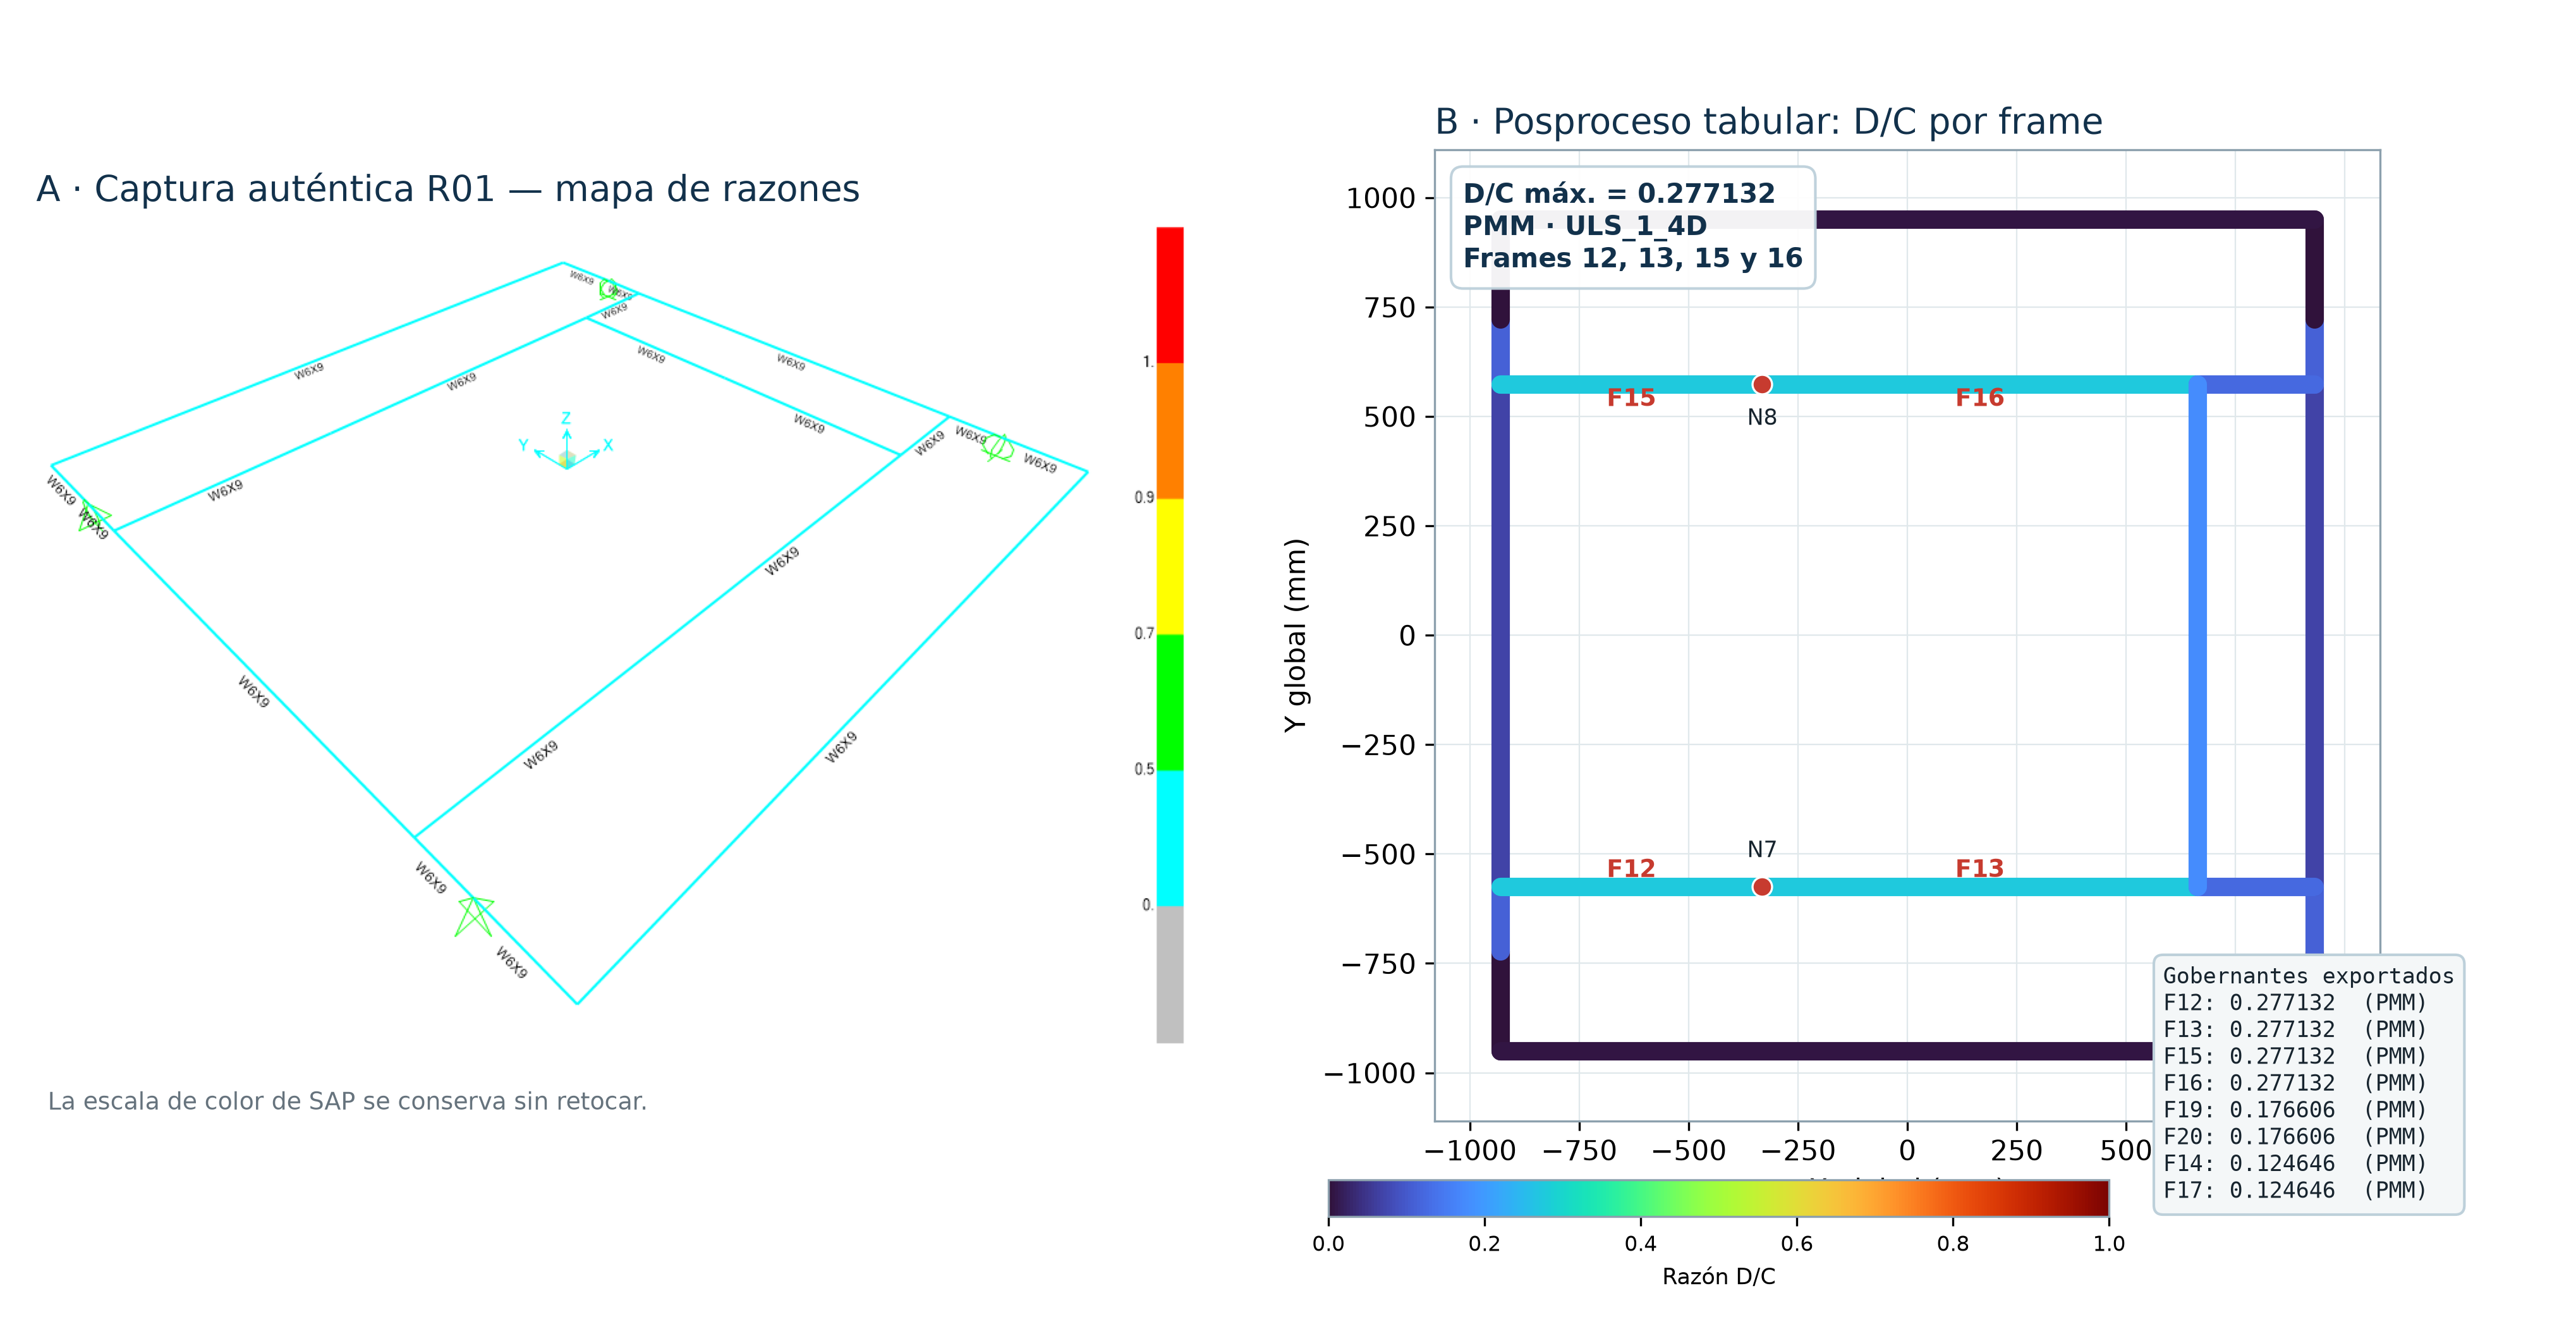
\includegraphics[width=\textwidth]{images/sap/04_VERIFICACION_RESISTENTE_R01_recorte.png}
\caption{Verificación resistente del bastidor con AISC 360-16 en SAP2000: razones demanda/capacidad por barra en la combinación ULS. Captura de la corrida de referencia.}
\label{fig:anx-resistencia-r01}
\end{figure}

\subsection{Respaldo del cálculo manual}
\label{sec:respaldo-complementario}

El caso manual de la Sección~\ref{sec:memoria-soporte} se contrasta con las hojas de coordenadas, cargas, reacciones y desplazamientos de \path{evidencias/N3_R01/R01_SAP_ORIGINAL.xlsx}. No se dispone del libro complementario \path{calculos/CALCULOS_SOPORTE_N3_N4_N5.xlsx}, citado como soporte de la hoja \emph{Contacto N3}; por ello, la extensión automática de ese desarrollo no forma parte de los entregables verificables. El libro mecánico de la revisión mecánica 5 contiene las hojas \emph{Ruedas}, \emph{PAD\_Contacto} y \emph{Auditoria\_R01}, pero responde a sus propios casos y no recalcula las corridas de cuatro y cinco apoyos.

\section{Libro mecánico de la revisión mecánica 5}
\label{sec:traza-ruedas-riel}

Las cargas de ruedas y riel de la Sección~\ref{sec:ruedas-rieles} se obtuvieron con el cálculo mecánico de esa revisión. La Tabla~\ref{tab:traza-ruedas-riel} relaciona cada magnitud con su hoja y celda en \path{evidencias/N3_R05/02_CALCULOS_EDITABLES_N3_R05.xlsx}. El procedimiento se desarrolla en \path{evidencias/N3_R05/01_CALCULO_R05_REPRODUCIBLE.py} y los resultados se almacenan en \path{evidencias/N3_R05/19_RESULTADOS_NUMERICOS_R05.json}. Este cálculo es independiente de la corrida estructural de referencia.

\begingroup
\small\singlespacing
\begin{longtable}{P{3.4cm}P{4.0cm}P{5.1cm}}
\caption{Trazabilidad de ruedas y riel en el libro mecánico de la revisión mecánica 5}\label{tab:traza-ruedas-riel}\\
\toprule
\textbf{Magnitud} & \textbf{Hoja y celda} & \textbf{Valor y alcance} \\
\midrule
Masa de cálculo & \texttt{Entradas!C7} & 3500 kg; escenario de diseño \\
Masa estimada & \texttt{Masa\_CG!B20} & 3439,831288 kg; balance de masas \\
Peso de cálculo & \texttt{Ruedas!B19} & 34,335 kN \\
Carga de servicio & \texttt{Ruedas!B7} & 21,865488 kN; factor 1,15 \\
Carga resistente local & \texttt{Ruedas!B8} & 26,618855 kN; factor 1,40 \\
Reacción de instalación & \makecell[l]{\texttt{Riel\_Envolvente}\\\texttt{B13}} & 26,741372 kN; apoyo del riel \\
Momento del vano simple & \makecell[l]{\texttt{Riel\_Envolvente}\\\texttt{B16}} & 3956529,787 N\,mm; carga resistente \\
Esfuerzos de cabeza y base & \makecell[l]{\texttt{Riel\_Envolvente}\\\texttt{B17:B18}} & 146,538140 y 95,338067 MPa \\
Flecha de servicio & \makecell[l]{\texttt{Riel\_Envolvente}\\\texttt{B19}} & 0,531864 mm; carga de servicio \\
\bottomrule
\end{longtable}
\endgroup

El caso manual se identifica como \texttt{3C\_W1\_MP} en el código y en \texttt{wheel\_cases} del archivo de resultados. El libro identifica primero el caso simétrico \texttt{3C-03}, con la rueda 3 ausente y $e_x=e_y=+100$ mm; ambos alcanzan el mismo máximo sin factor, de 19,013468 kN. Las funciones \texttt{wheel\_cases} y \texttt{rail\_envelope} contienen los barridos restantes. El bloque \texttt{rail.governing\_continuous} localiza la reacción de instalación en el riel derecho, apoyo 2, caso \texttt{3C\_W4\_PM}, con el centro de la mesa en $Y=-3320{,}038$ mm y una carga de rueda de 26,618855 kN en $Y=-4042{,}038$ mm. El mínimo de la sensibilidad continua, $-3{,}691891$ kN, corresponde a los apoyos riel--base y no al contacto rueda--riel; esa sensibilidad usa restricciones bilaterales y no valida la retención ni el diseño civil.

La configuración vigente, con doce apoyos por riel, se recalculó en la revisión de integración (\path{estructural/integracion_R06/00_ANALISIS_PREVIOS_2026-09-24/J2_soportes_riel_recalculo.md}): reacción máxima de apoyo de 26,623 kN y mínima de $-3{,}779$ kN en ULS, esfuerzos de cabeza y base de 97,92 y 63,71 MPa y flechas entre apoyos de 0,260 mm en servicio y 0,317 mm en ULS, valores resumidos en la Tabla~\ref{tab:ruedas-rieles}.

\section{Modelo de mojado: configuración y verificación}
\label{sec:anx-cfd}

La Tabla~\ref{tab:anx-cfd-config} reúne la configuración del modelo de mojado de la Sección~\ref{sec:resultados-aspersion}. Los journals, las tablas de inyección, las transcripciones y los resultados se conservan en \path{cfd/02_configuracion_base_22/} y \path{cfd/03_configuracion_propuesta_24/}; los casos de Fluent y los impactos exportados no se publican por su tamaño. Los guiones \path{rayos_r05.py}, \path{post_kpi.py}, \path{combinar_kpi.py}, \path{tabla_k1k6.py} y \path{balance_global_22.py} calculan las máscaras de sombra, los indicadores y el balance. Un recálculo independiente de los indicadores de dosis, uniformidad, zona seca, transferencia e impulso a partir de los impactos reprodujo los valores con diferencias menores que 1\,\%; las máscaras y el acceso geométrico se reprodujeron exactamente al ejecutar de nuevo el mismo trazado de rayos, lo que confirma su reproducibilidad, pero no es un método independiente.

\begingroup
\small\singlespacing
\setlength{\tabcolsep}{4pt}
\begin{longtable}{@{}>{\raggedright\arraybackslash}p{3.4cm}>{\raggedright\arraybackslash}p{\dimexpr\textwidth-3.4cm-4\tabcolsep\relax}@{}}
\caption{Configuración del modelo de mojado}\label{tab:anx-cfd-config}\\
\toprule
\textbf{Aspecto} & \textbf{Configuración}\\
\midrule\endfirsthead
\toprule
\textbf{Aspecto} & \textbf{Configuración}\\
\midrule\endhead
\bottomrule\endlastfoot
Programa & ANSYS Fluent 2026 R1, versión estudiantil, limitada a 1\,048\,576 celdas\\
Régimen & Transitorio; $\Delta t=5\times10^{-5}$ s con 10 iteraciones por paso\\
Fase continua & Aire con turbulencia $k$--$\varepsilon$ estándar a 76,24 kPa (escenario de 2335 m)\\
Fase discreta & Lagrangiana, acoplada en dos vías, sin dispersión turbulenta estocástica; líquido de 982,12 kg/m$^3$ a 62~$^\circ$C\\
Inyección & Abanico de 50$^\circ$ con 2$^\circ$ de espesor; gotas con distribución de Rosin--Rammler de diámetro característico 300 µm y exponente 2,5, supuesta; velocidad de salida $0{,}95\sqrt{2p/\rho}$, de unos 27,5 m/s; caudal y presión de cada boquilla según la red de 22 boquillas; 600 trayectorias por plano y tres planos de espesor (1200 en las boquillas inferiores). En la configuración propuesta, las cuatro boquillas inferiores tienen un abanico de 15$^\circ$, interpolado a 16,8$^\circ$ a 4 bar (hipótesis), y los caudales de la red de 24 boquillas\\
Paredes y fronteras & Retención de la gota en el primer impacto; fronteras abiertas a la presión del sitio\\
Dominios & Sector de las boquillas laterales e inferior exterior del brazo exterior A (430\,560 celdas) y el mismo sector para el brazo B; sector de 90$^\circ$ para la boquilla inferior de la lanza (197\,280); sector de la cara superior (237\,552); dominio polar completo del agujero (512\,130)\\
Malla & Hexaédrica estructurada; tamaño máximo de 4 mm en dirección radial, 0,5$^\circ$ en la angular y 5 mm en la axial\\
Movimiento del aplicador & Detenido; dosis por vuelta a 1,7 rpm integrando la huella sobre la circunferencia\\
Obstáculos & Apoyos sectoriales, topes y vigas como máscaras de sombra por trazado de rayos, con la geometría del soporte\\
Posproceso & Indicadores por bandas de 10 mm (definición principal) y de 2 mm (complementaria)\\
\end{longtable}
\endgroup

La Figura~\ref{fig:anx-dominio} muestra el dominio sectorial de $\pm12^\circ$ y la malla hexaédrica del sector de las boquillas laterales y de la inferior exterior, con sus fronteras abiertas. La Figura~\ref{fig:anx-aire} ilustra el efecto que incorpora el acoplamiento en dos vías: el chorro arrastra el aire hacia la pared, y ese aire frena las gotas de la parte baja del diámetro exterior.

\begin{figure}[htbp]
\centering
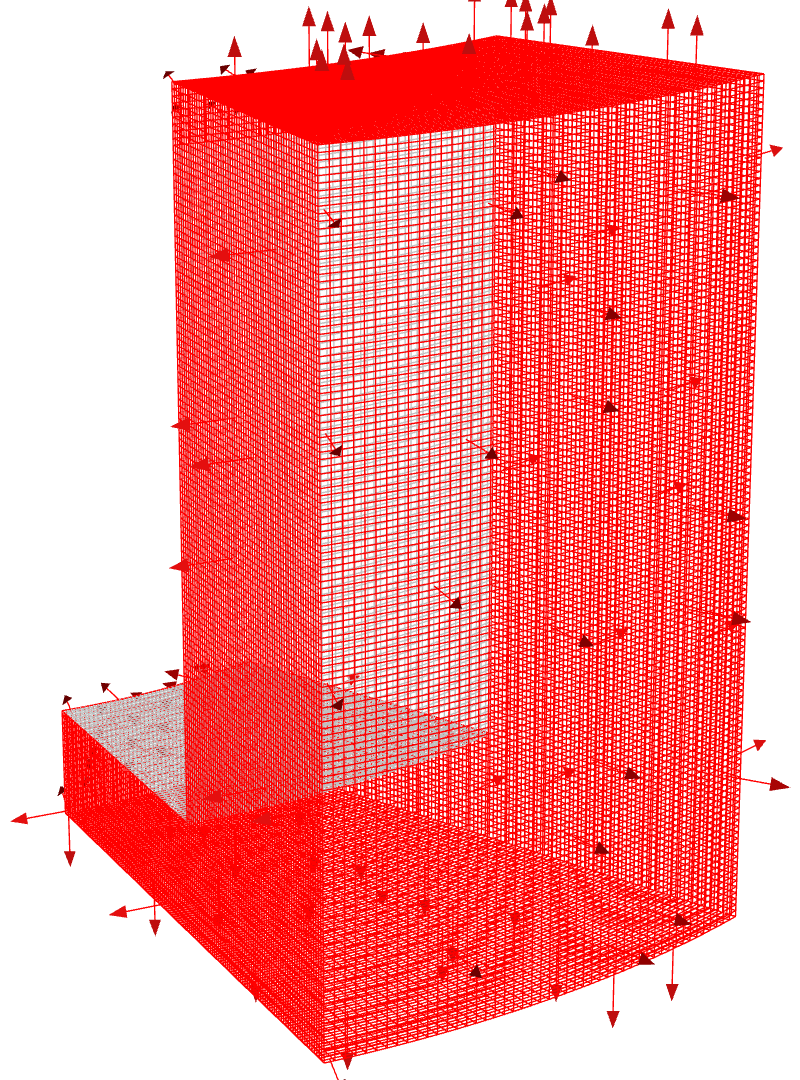
\includegraphics[width=0.55\textwidth]{fluent_dominio_malla_od.png}
\caption[Dominio y malla del sector de las boquillas laterales e inferior exterior]{Dominio de cálculo y malla hexaédrica del sector de $\pm12^\circ$ de las boquillas laterales y de la inferior exterior de un brazo (diámetro exterior y cara inferior), vista isométrica; las flechas señalan las fronteras abiertas. Elaboración propia, ANSYS Fluent 2026 R1 (licencia Student); imagen recortada al área de interés.}
\label{fig:anx-dominio}
\end{figure}

\begin{figure}[htbp]
\centering
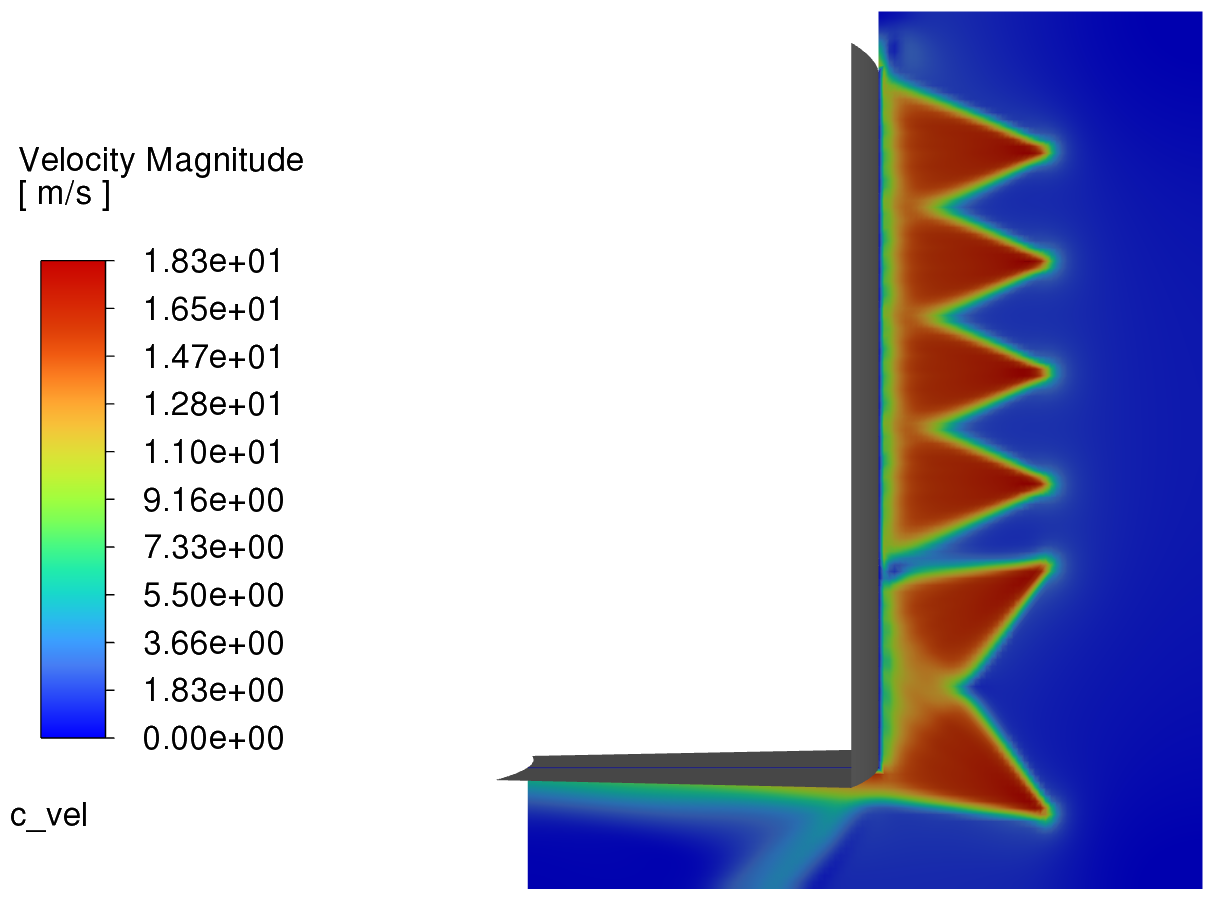
\includegraphics[width=0.70\textwidth]{fluent_aire_arrastrado_od.png}
\caption[Velocidad del aire arrastrado por los chorros]{Velocidad del aire en el plano de los abanicos de las boquillas laterales y de la inferior exterior de un brazo, configuración base. Es un campo de la fase continua, no un indicador. La escala de color es la magnitud de la velocidad en m/s (rótulo del programa en inglés). Elaboración propia, simulación en ANSYS Fluent 2026 R1 (licencia Student); imagen recortada al área de interés.}
\label{fig:anx-aire}
\end{figure}

La velocidad de salida se calculó con un coeficiente de 0,95 sobre la velocidad ideal, lo que da 27,11--27,59 m/s. Como contraste, la continuidad con el orificio equivalente de catálogo, de 0,109 pulgadas (2,77 mm), y el caudal de cada toma da 25,24--25,68 m/s, un 7\,\% menos; ese orificio implica un coeficiente de descarga de 0,884 (Sección~\ref{sec:man-asp-boquilla}). El modelo de mojado registró velocidades normales de impacto de 23,0 a 23,4 m/s en el diámetro exterior, la cara superior y el agujero, por debajo de ambas estimaciones, como corresponde al frenado aerodinámico de las gotas en los 126 a 185 mm de vuelo. Como el impulso es proporcional a la velocidad de las gotas a igual caudal, adoptar la velocidad por continuidad reduciría $\bar J$ en un 7\,\% como máximo; la dosis y la transferencia dependen sobre todo del caudal, que es el mismo en ambos casos.

La Tabla~\ref{tab:verificacion-cfd} reúne los cambios de los indicadores entre las dos mallas más finas, con el paso de tiempo a la mitad y con el dominio ampliado.

\begin{table}[htbp]
\centering\small\singlespacing
\caption{Verificación numérica del modelo de mojado: cambio respecto de la corrida base}
\label{tab:verificacion-cfd}
\begin{tabular}{lcccc}
\toprule
\textbf{Estudio} & \textbf{$\bar D$} & \textbf{CV (absoluto)} & \textbf{$\bar J$} & \textbf{$\eta$}\\
\midrule
Malla fina, cara superior & $-0{,}08$\,\% & $-0{,}0039$ & $+0{,}54$\,\% & $-0{,}07$\,\%\\
Malla fina, diámetro exterior & $-0{,}11$\,\% & $-0{,}0002$ & $+0{,}75$\,\% & $-0{,}12$\,\%\\
Malla fina, cara inferior (exterior) & $+0{,}61$\,\% & $-0{,}0151$ & $+1{,}01$\,\% & $+0{,}57$\,\%\\
Malla fina, cara inferior (lanza) & $-0{,}19$\,\% & $+0{,}0012$ & $+0{,}30$\,\% & $-0{,}18$\,\%\\
Paso de tiempo a la mitad & $\leq0{,}01$\,\% & $\leq0{,}0001$ & $\leq0{,}04$\,\% & $\leq0{,}02$\,\%\\
Dominio ampliado & $\leq0{,}14$\,\% & $\leq0{,}0084$ & $\leq0{,}27$\,\% & $\leq0{,}02$\,\%\\
\bottomrule
\end{tabular}
\par\smallskip\footnotesize
$\bar D$: dosis media; CV: coeficiente de variación; $\bar J$: impulso medio; $\eta$: transferencia.
\end{table}

La Tabla~\ref{tab:anx-gci} contiene el estudio de malla de tres niveles de la configuración base y la Figura~\ref{fig:anx-verificacion-cfd}, la dosis media y la presión de huella de cada malla normalizadas con las de la malla fina. Cuando el cambio entre las dos mallas finas es menor que el ruido entre corridas equivalentes de los brazos exteriores A y B, el índice de convergencia de malla no es interpretable y basta con comprobar que el cambio sea pequeño.

\begin{table}[htbp]
\centering\small\singlespacing
\setlength{\tabcolsep}{2.5pt}
\caption{Estudio de malla del modelo de mojado: índice de convergencia de la malla fina}
\label{tab:anx-gci}
\begin{tabular}{lcccccc}
\toprule
\textbf{Dominio} & \textbf{Celdas (miles)} & \textbf{$r_{21}$; $r_{32}$} & \textbf{$\bar D$} & \textbf{CV} & \textbf{$\bar J$} & \textbf{$\eta$}\\
\midrule
Cara superior & 112 / 238 / 465 & 1,251; 1,283 & 0,07\,\% & 2,20\,\% & 1,47\,\% & 0,05\,\%\\
Diámetro exterior & 203 / 431 / 847 & 1,253; 1,286 & 0,30\,\% & 0,68\,\% & 4,45\,\% & 0,25\,\%\\
Cara inferior, exterior* & 203 / 431 / 847 & 1,253; 1,286 & 3,92\,\% & 12,55\,\% & 4,88\,\% & 5,82\,\%\\
Cara inferior, lanza & 91 / 197 / 381 & 1,246; 1,295 & 0,18\,\% & 0,06\,\% & 1,44\,\% & 0,17\,\%\\
Borde del agujero, lanza & 91 / 197 / 381 & 1,246; 1,295 & 0,11\,\% & 1,07\,\% & 1,62\,\% & 0,14\,\%\\
\bottomrule
\end{tabular}
\par\smallskip\footnotesize
*Cambios entre mallas dentro del ruido entre los brazos A y B: índice no interpretable. Procedimiento de \cite{celik2008}.
\end{table}

\begin{figure}[htbp]
\centering
\begin{minipage}[t]{0.49\textwidth}\centering
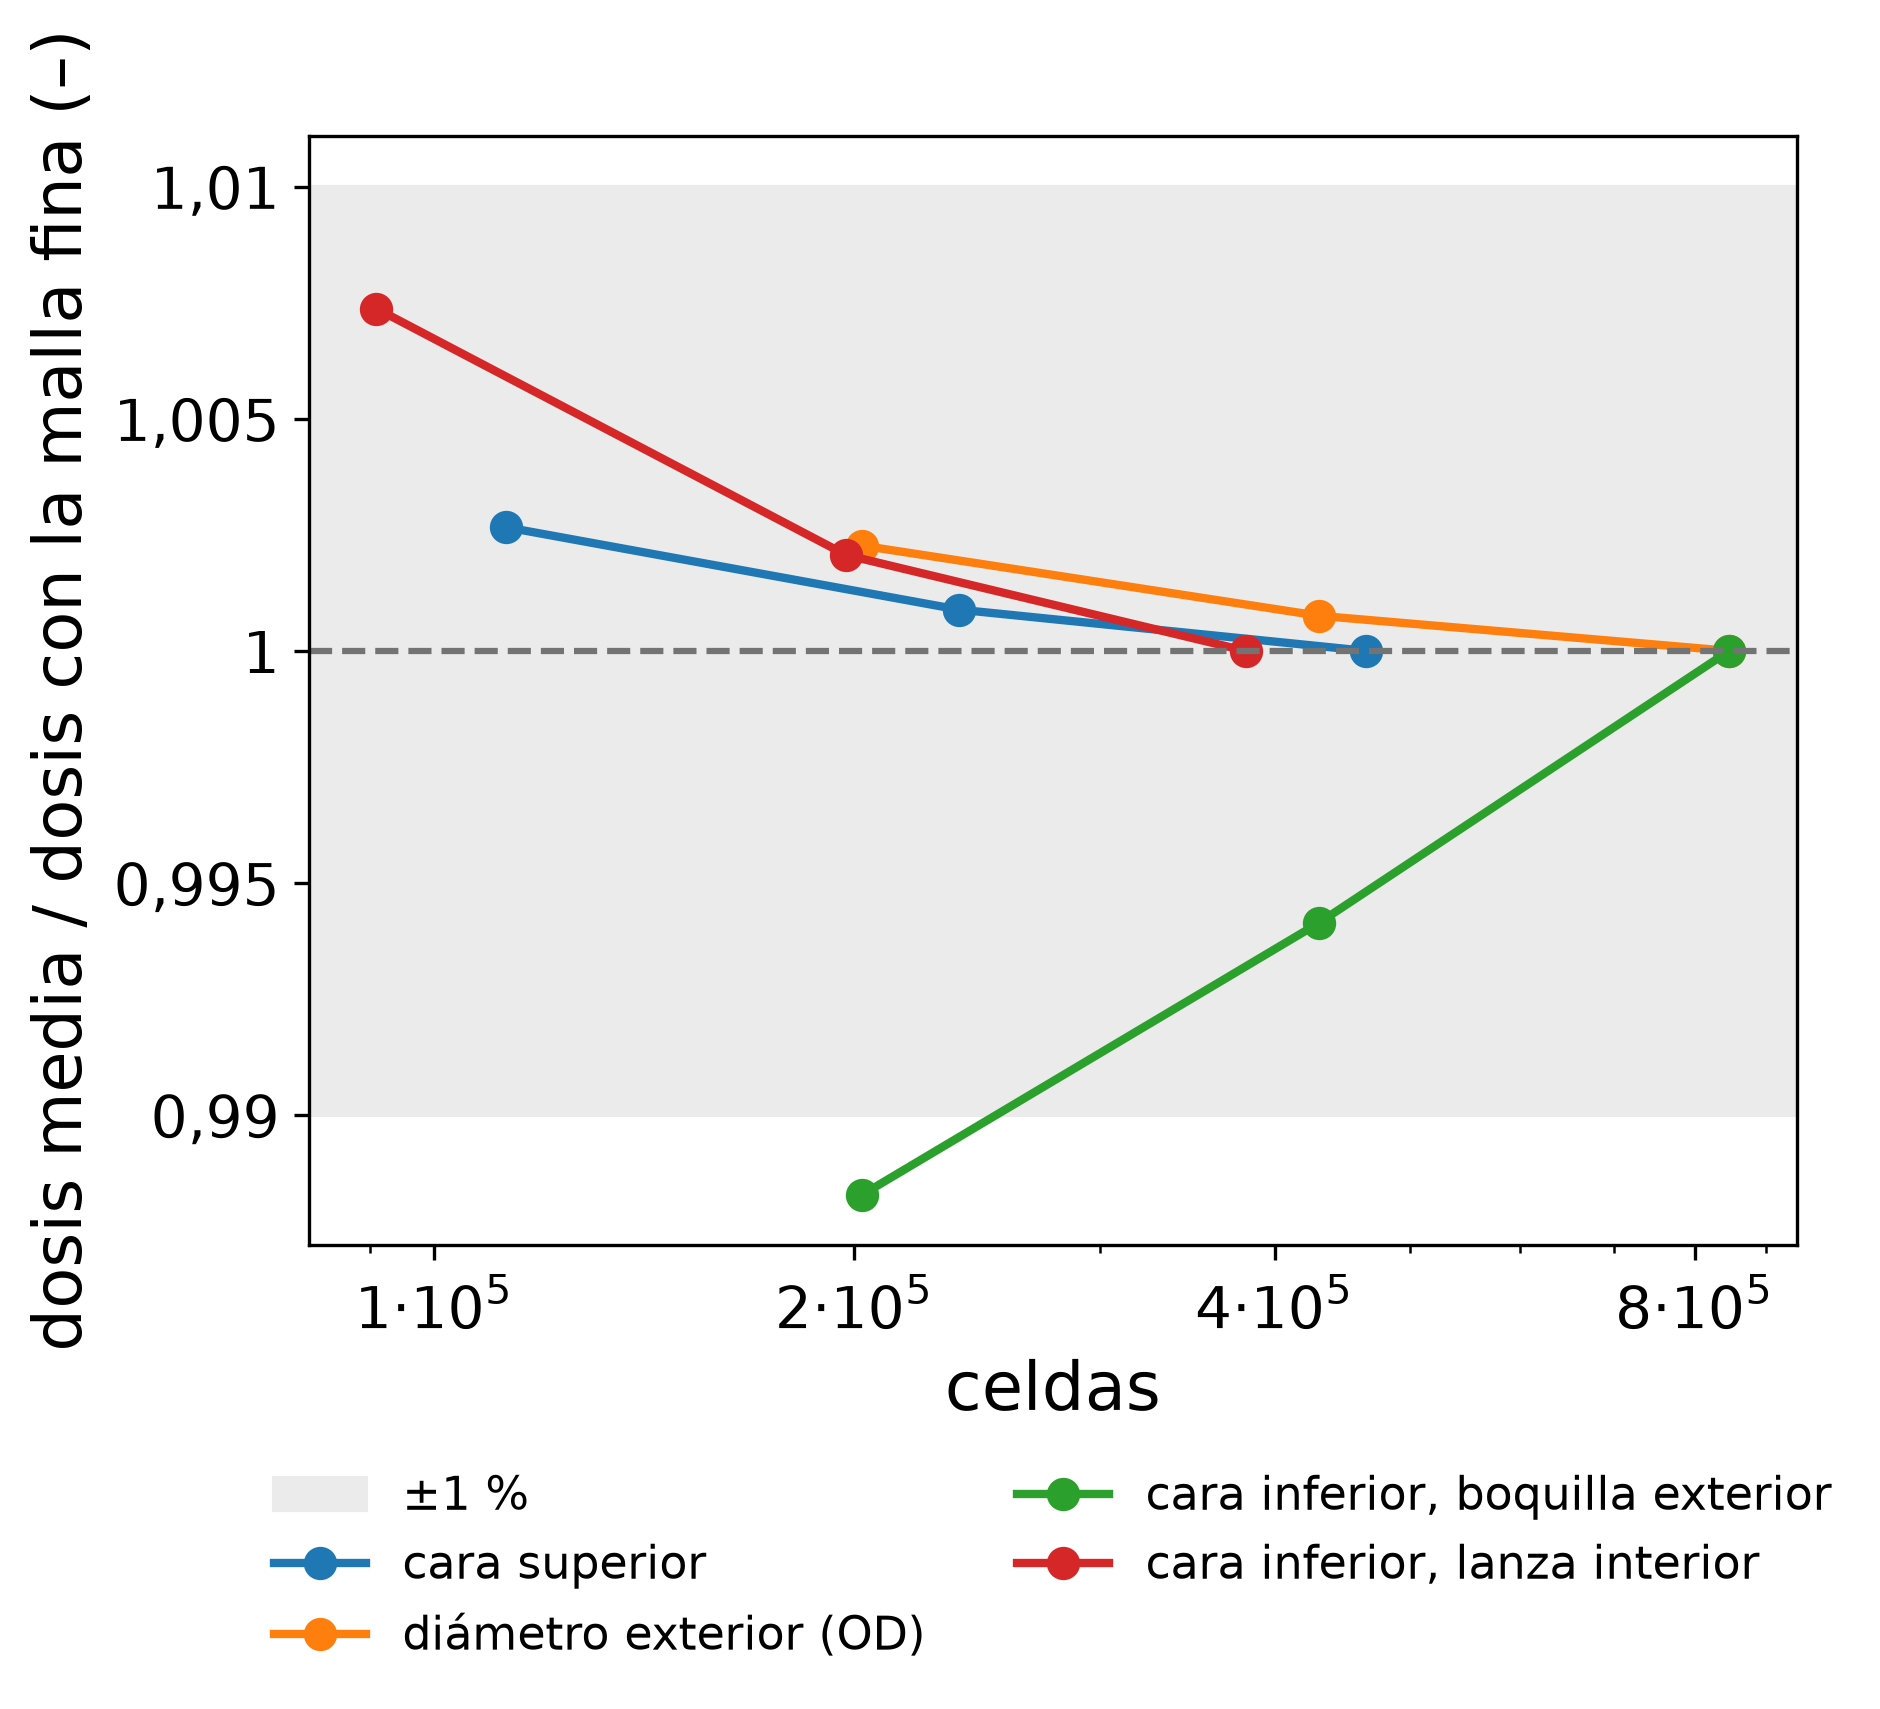
\includegraphics[width=\linewidth]{F11_DPM_dosis_media_frente_a_malla.png}\par\small (a)
\end{minipage}\hfill
\begin{minipage}[t]{0.49\textwidth}\centering
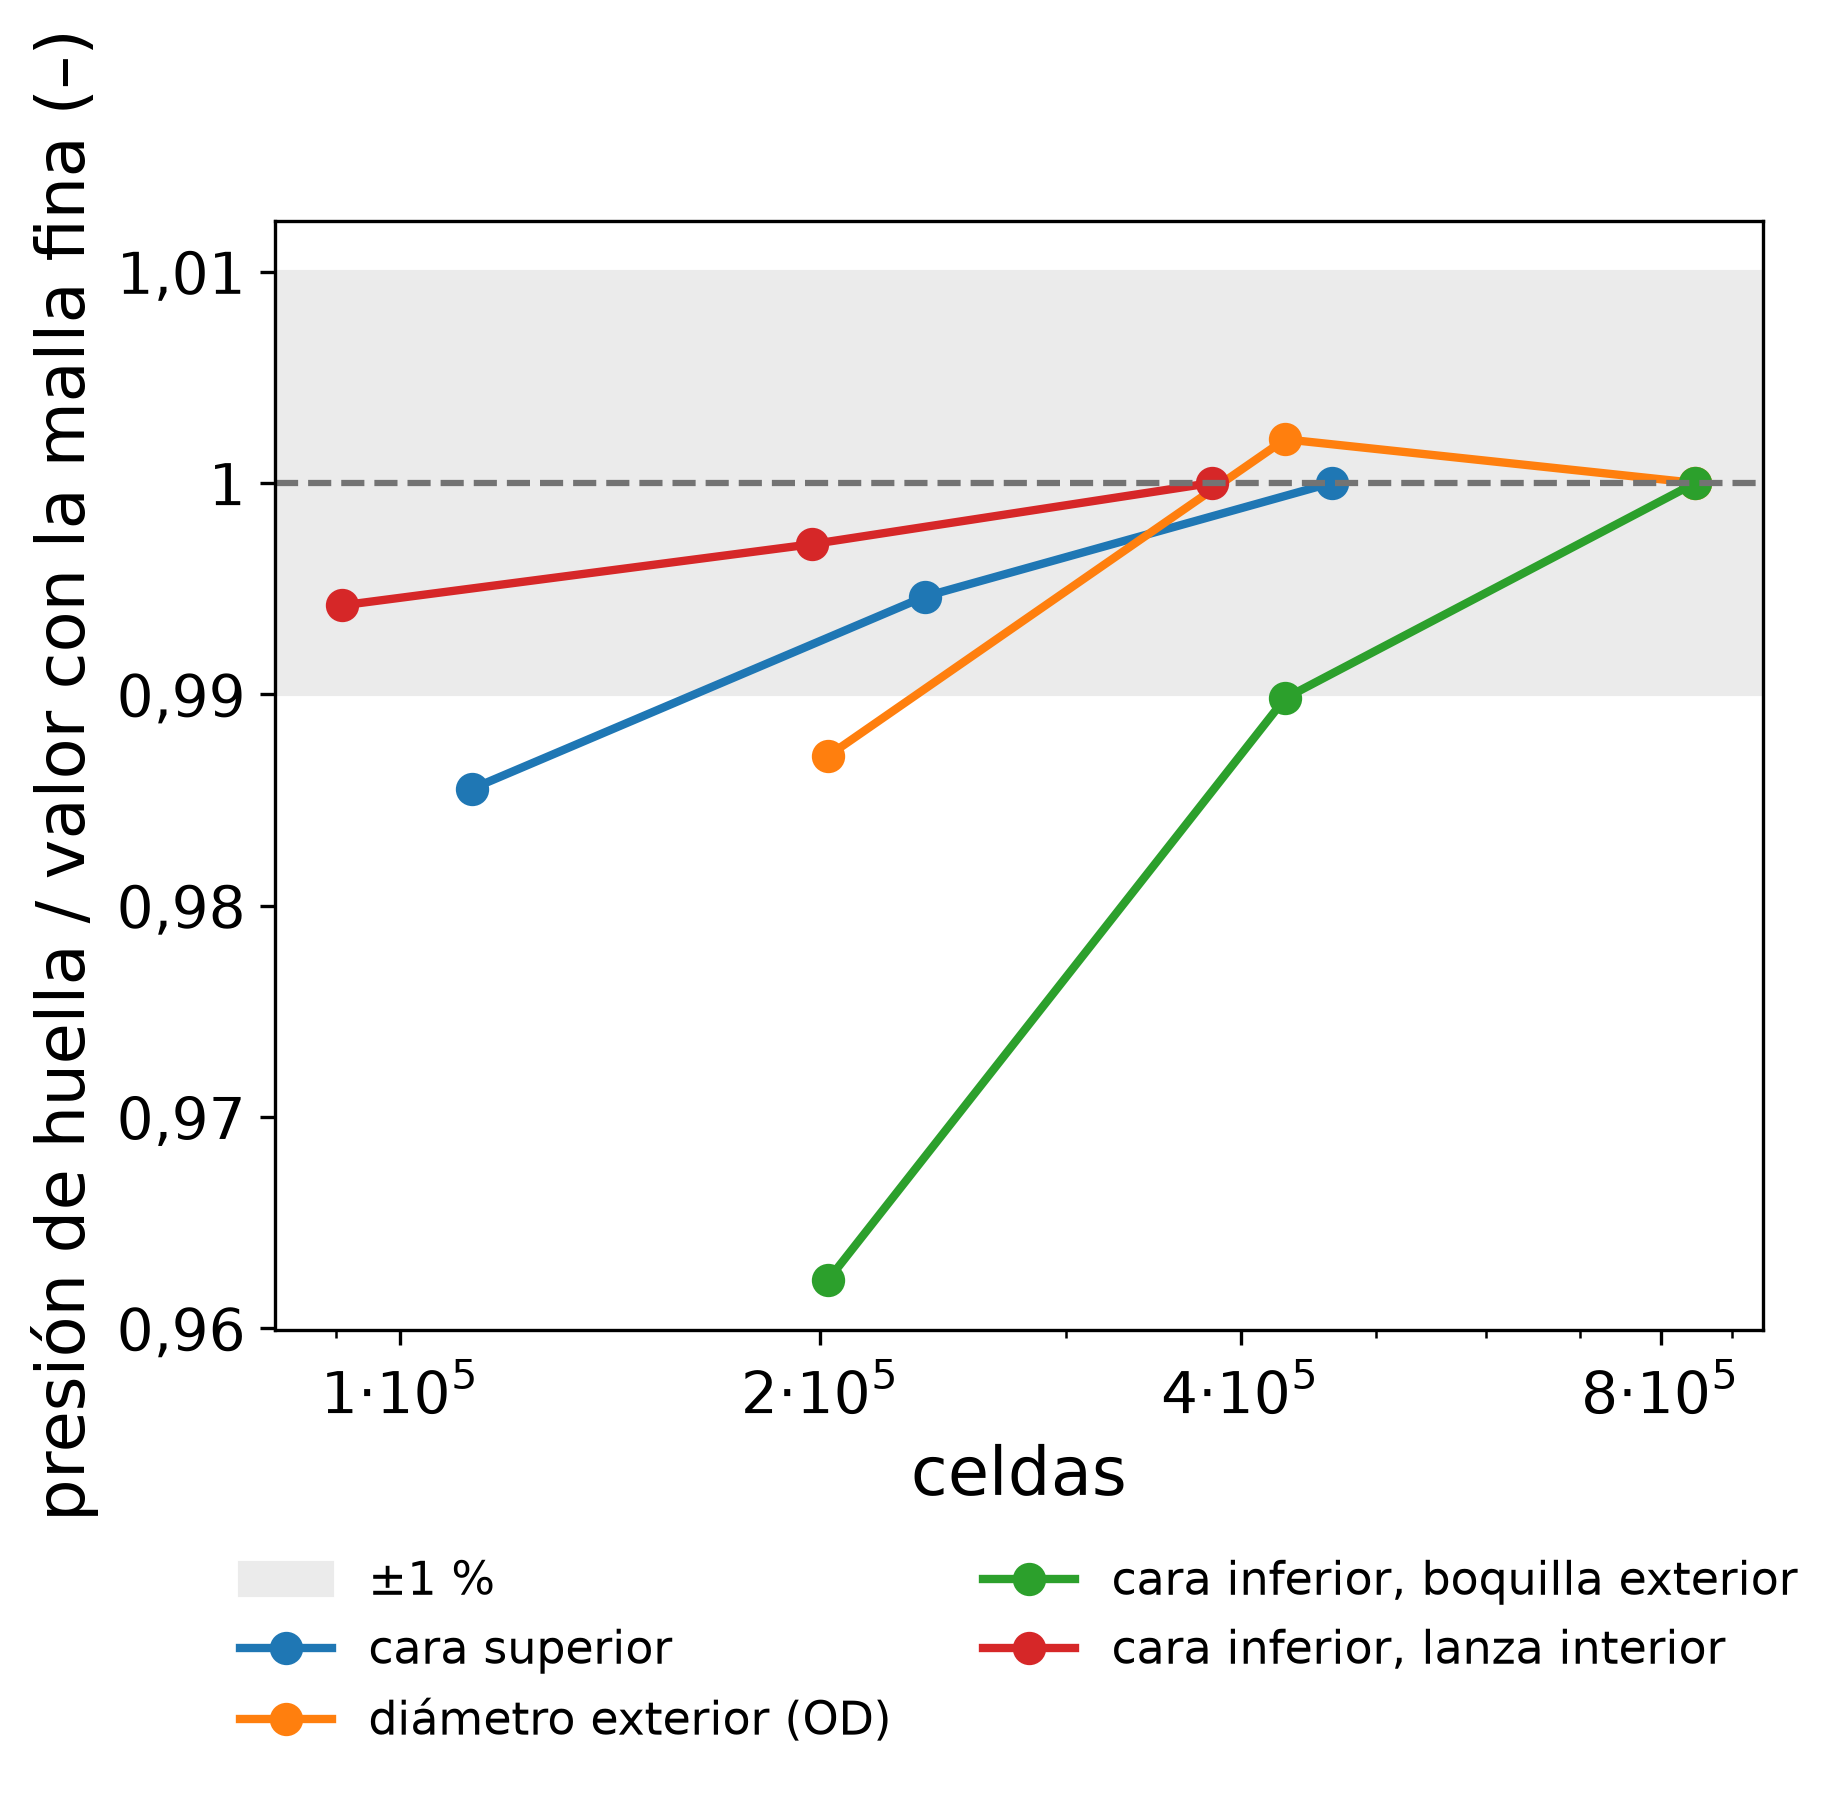
\includegraphics[width=\linewidth]{F12_DPM_presion_huella_frente_a_malla.png}\par\small (b)
\end{minipage}
\caption[Verificación de malla del modelo de mojado de la configuración base]{Verificación de malla de la configuración base: (a) dosis media y (b) presión de huella de cada malla, normalizadas con las de la malla fina. Verificación numérica, no validación. Elaboración propia con los resultados de ANSYS Fluent.}
\label{fig:anx-verificacion-cfd}
\end{figure}

En esa configuración el paso de tiempo fue fijo, de modo que el número de Courant de las gotas creció con el refinamiento: 0,27, 0,34 y 0,43 en las tres mallas. Para descartar que ese crecimiento afectara el estudio, las mallas gruesa y fina de los tres dominios se repitieron con el paso de tiempo ajustado para mantener el Courant de gota en 0,34 (0,27 en la cara superior). Los cambios entre las dos mallas más finas fueron los mismos que con el paso fijo: las diferencias entre ambas series no pasaron de 0,03 puntos porcentuales en la dosis media ni de 0,07 en el impulso medio, y los balances de masa quedaron entre 0,02 y 0,14\,\%. En la configuración propuesta se ajustó el paso de tiempo de cada malla para mantenerlo cerca de 0,339 desde el principio (Sección~\ref{sec:resultados-aspersion}).

La Tabla~\ref{tab:anx-mascaras} compara el método de máscaras con una corrida en la que un apoyo sectorial se incluyó en la malla, y la Tabla~\ref{tab:anx-puente} resume el caso puente entre OpenFOAM y Fluent en el agujero.

\begin{table}[htbp]
\centering\small\singlespacing
\caption{Sombras por trazado de rayos frente a un apoyo incluido en la malla: fracción del caudal de la boquilla que llega a cada destino}
\label{tab:anx-mascaras}
\begin{tabularx}{\textwidth}{@{}YP{2.6cm}P{3.4cm}@{}}
\toprule
\textbf{Boquilla y destino} & \textbf{Trazado de rayos (\%)} & \textbf{CFD con el apoyo en la malla (\%)}\\
\midrule
Inferior exterior $\rightarrow$ apoyos sectoriales & 18,0 & 16,9\\
Inferior exterior $\rightarrow$ cara inferior, sin apoyos & 20,7 & 21,0\\
Inferior exterior $\rightarrow$ cara inferior, con apoyos & 4,0 & 4,5\\
Lateral 5 $\rightarrow$ apoyos sectoriales & 12,7 & 9,2\\
\bottomrule
\end{tabularx}
\par\smallskip\footnotesize
Configuración base. Verificación del método, no validación.
\end{table}

\begin{table}[htbp]
\centering\small\singlespacing
\caption{Caso puente del agujero: OpenFOAM frente a ANSYS Fluent}
\label{tab:anx-puente}
\begin{tabular}{@{}>{\raggedright\arraybackslash}p{4.6cm}cccc@{}}
\toprule
\textbf{Indicador} & \textbf{OpenFOAM} & \textbf{Fluent} & \textbf{Diferencia} & \textbf{Criterio}\\
\midrule
Caudal depositado (kg/s) & 0,7835 & 0,7814 & $-0{,}26$\,\% & ---\\
Dosis media (kg\,m$^{-2}$ por vuelta) & 18,809 & 18,759 & $-0{,}27$\,\% & $\leq5$\,\%\\
Coeficiente de variación & 0,3397 & 0,3362 & $-0{,}0035$ & $\leq0{,}03$\\
Zona seca (\%) & 0 & 0 & 0 & 0 en ambos\\
Curvas de cobertura, diferencia máxima & --- & --- & 1,33 puntos & $\leq2$ puntos\\
\bottomrule
\end{tabular}
\end{table}

\begin{figure}[htbp]
\centering
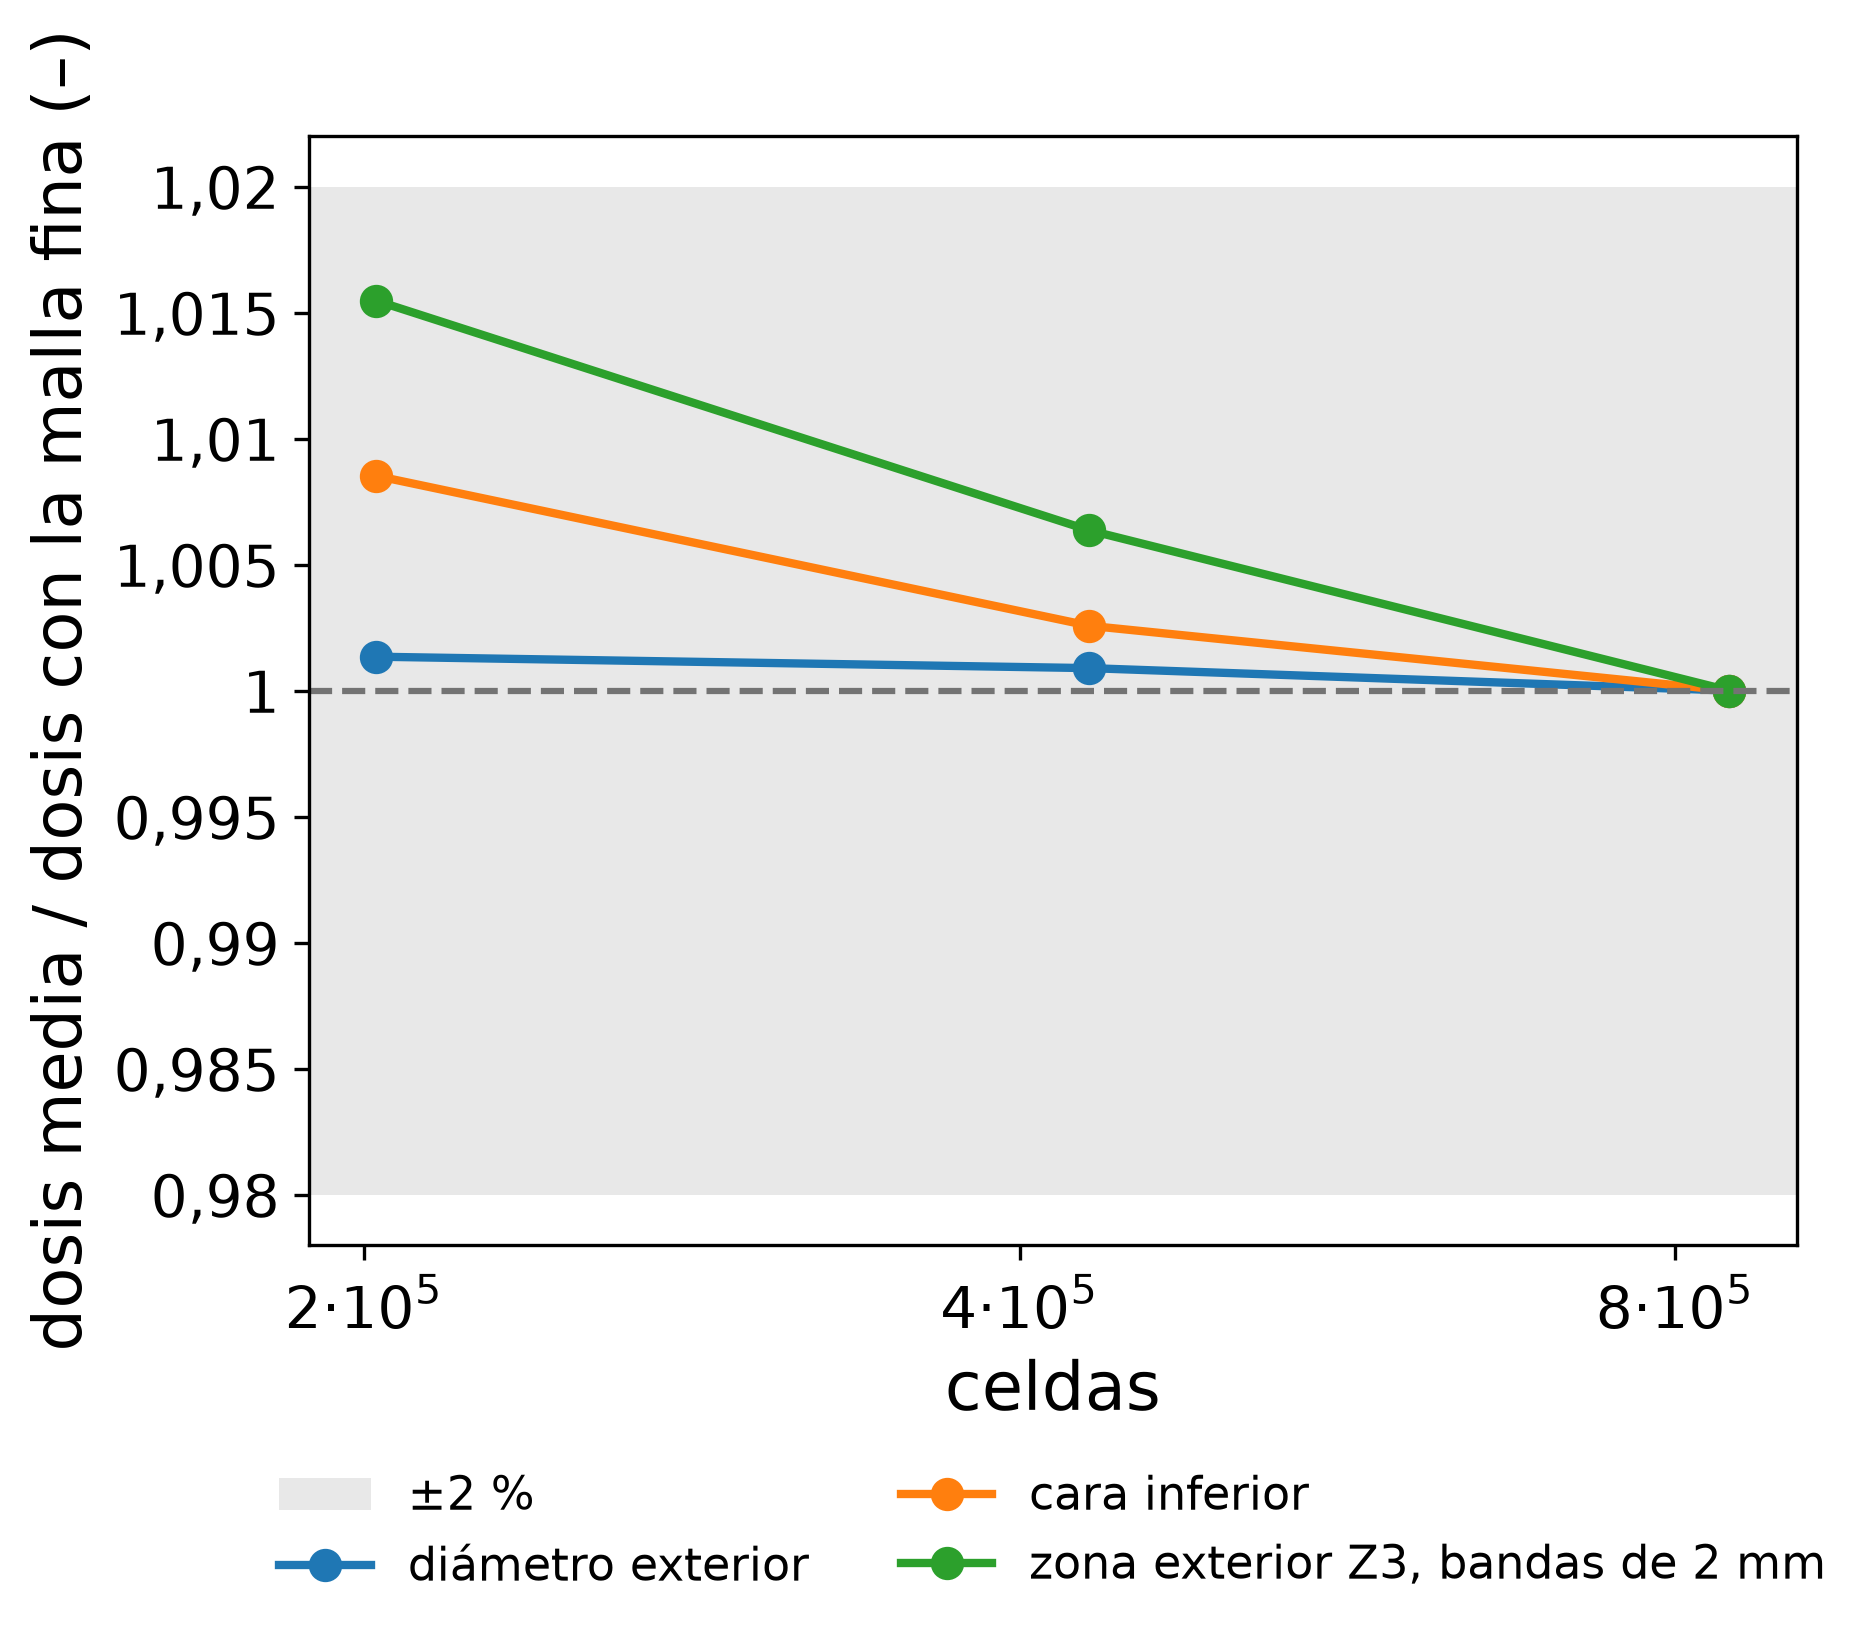
\includegraphics[width=0.55\textwidth]{fig_malla_configuracion_propuesta.png}
\caption{Dosis media de la configuración propuesta de 24 boquillas con tres mallas, normalizada con la de la malla fina. Elaboración propia con los datos exportados de ANSYS Fluent.}
\label{fig:cfd-malla-propuesta}
\end{figure}

\section{Tiempo de lavado y sombras de la cara inferior}
\label{sec:anx-tiempo-lavado}

La dosis acumulada después de $N$ vueltas en una banda o en una celda es $N\,D$, con $D$ la dosis por vuelta de la Ecuación~\eqref{eq:teo-dosis}. El tiempo $t_{95}$ de la Tabla~\ref{tab:tiempo-lavado} es el menor número entero de vueltas para el que el 95\,\% del área accesible cumple $N\,D\geq D_{req}$, multiplicado por los 35,3 s de una vuelta. La lectura por bandas usa la dosis media de cada anillo de 10 mm. La lectura por celdas usa el mapa de 10 mm por 0,5$^\circ$ exportado del CFD con las máscaras de sombra, que distingue las zonas donde un apoyo o un tope tapa solo una parte de los chorros durante la vuelta.

\begin{table}[htbp]
\centering\small\singlespacing
\caption{Tiempo para que el 95\,\% del área accesible alcance la dosis requerida}
\label{tab:tiempo-lavado}
\begin{tabular}{@{}llccc@{}}
\toprule
\textbf{Superficie} & \textbf{Lectura} & \textbf{65 kg\,m$^{-2}$} & \textbf{183 kg\,m$^{-2}$} & \textbf{305 kg\,m$^{-2}$}\\
\midrule
Diámetro exterior & Bandas y celdas & 2,9 & 8,2 & 14,1\\
Cara superior & Bandas y celdas & 4,1 & 10,6 & 17,6\\
Agujero & Bandas y celdas & 2,9 & 8,2 & 14,1\\
Cara inferior & Bandas de 10 mm & 5,3 & 14,1 & 23,5\\
 & Celdas de 10 mm $\times$ 0,5$^\circ$ & 27,1 & 75,9 & $>120$\\
\bottomrule
\end{tabular}
\par\smallskip\footnotesize
Tiempos en minutos, en vueltas enteras de 35,3 s a 1,7 rpm y con un horizonte de 120 min; 24 boquillas, con la boquilla superior en su posición base. Las bandas toman la dosis media de cada anillo de 10 mm; las celdas resuelven además la posición angular y registran las sombras parciales de las bases de los apoyos sectoriales y de los topes.
\end{table}

En el diámetro exterior, la cara superior y el agujero no hay sombras parciales, y las dos lecturas coinciden. En la cara inferior, el 10,4\,\% del área accesible tiene un factor de sombra menor que 0,25 y el 3,2\,\%, entre 0,25 y 0,5; corresponden a las bases de los apoyos sectoriales y a los topes de retención. Por eso la curva por celdas de la Figura~\ref{fig:anx-tiempo-lavado} sube rápido hasta un 83\,\% del área y después avanza despacio: el último 12\,\% es la zona sombreada.

\begin{figure}[htbp]
\centering
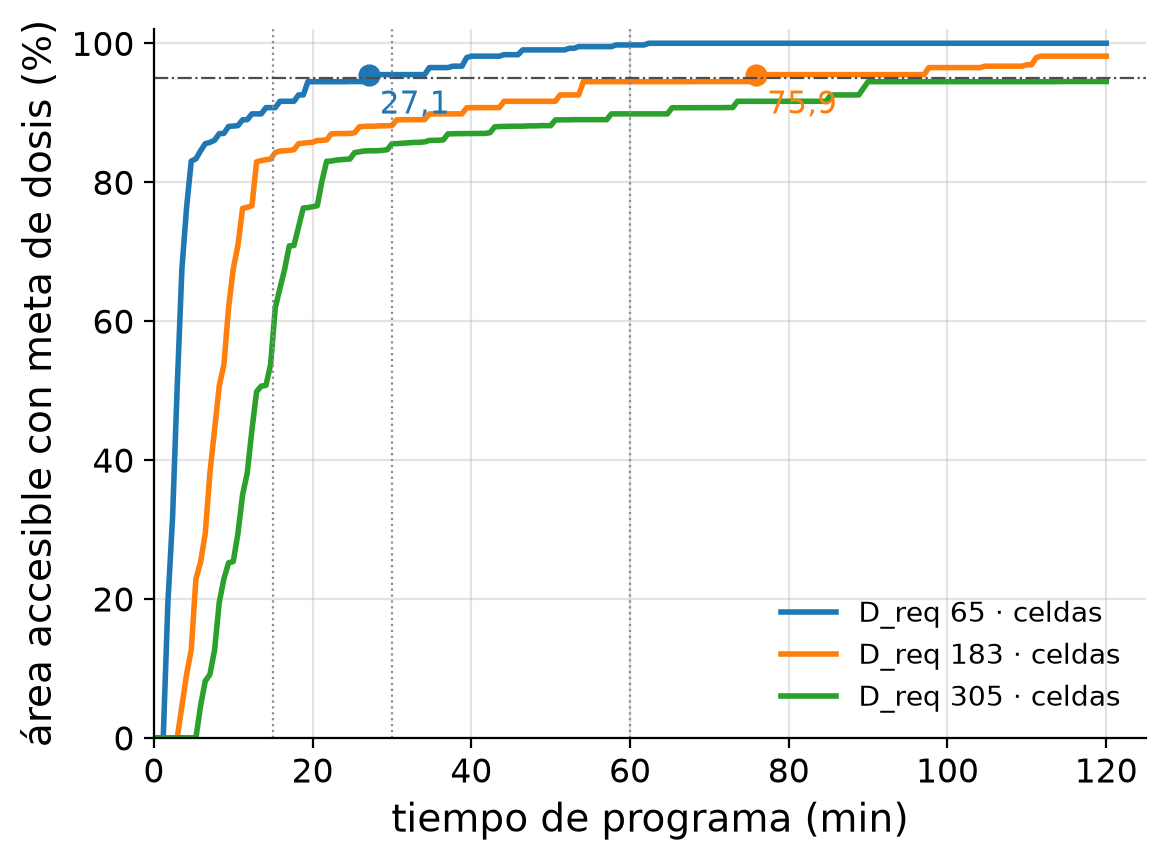
\includegraphics[width=0.62\textwidth]{asp_tiempo_lavado_cara_inferior.png}
\caption[Área de la cara inferior que alcanza la dosis requerida en función del tiempo]{Fracción del área accesible de la cara inferior que alcanza la dosis requerida en función del tiempo de lavado, lectura por celdas de 10 mm $\times$ 0,5$^\circ$, configuración de 24 boquillas. La línea horizontal marca el 95\,\% y los puntos, $t_{95}$. Elaboración propia con los datos exportados de ANSYS Fluent.}
\label{fig:anx-tiempo-lavado}
\end{figure}

\section{Acceso al interior del rodamiento armado}
\label{sec:anx-cavidad}

La geometría del interior se midió en el modelo del fabricante: las pistas exteriores forman una esfera de 669,04 mm de radio, y cada hilera tiene 23 rodillos abombados de 214 mm de longitud, con el eje inclinado 13$^\circ$ y la hilera inferior desfasada medio paso. El modelo no incluye la jaula. Desde cada boquilla se trazaron los tres planos de su abanico con 2400 rayos por plano y se giró el distribuidor en pasos de 0,1$^\circ$ a lo largo de una vuelta, con los apoyos sectoriales, los topes y las vigas como obstáculos; dentro del rodamiento, cada rayo avanzó en pasos de 1 mm hasta tocar un aro o un rodillo. Una superficie cuenta como visible si algún rayo la toca en alguna posición del distribuidor. La unión de las huellas converge despacio con la densidad de rayos: el área visible fue de 16,6\,\% con 150 rayos por plano, 22,5\,\% con 600 y 24,3\,\% con 2400, que es el valor que se informa (Tabla~\ref{tab:anx-cavidad}).

\begin{table}[htbp]
\centering\small\singlespacing
\caption{Área de rodillos y pistas con línea de vista desde las boquillas, rodamiento armado}
\label{tab:anx-cavidad}
\begin{tabularx}{\textwidth}{@{}Yc@{}}
\toprule
\textbf{Zona} & \textbf{Área visible (\%)}\\
\midrule
Rodillos y pistas, total & 24,3\\
Hilera superior: superficie lateral de los rodillos & 23,9\\
Hilera superior: extremo de los rodillos hacia la cara & 95,1\\
Hilera inferior: superficie lateral de los rodillos & 0,35\\
Hilera inferior: extremo de los rodillos hacia la cara & 49,4\\
Pista exterior, mitad superior & 66,1\\
Pista exterior, mitad inferior & 16,2\\
Pista interior, mitad superior & 30,5\\
Pista interior, mitad inferior & 1,9\\
\bottomrule
\end{tabularx}
\par\smallskip\footnotesize
Trazado de rayos del primer impacto desde las 24 boquillas, sin la jaula: los valores son cotas superiores. No incluye el escurrimiento ni la película que bajan desde la hilera superior.
\end{table}

La Figura~\ref{fig:anx-cavidad} muestra por qué. Las boquillas superiores entran por la ventana anular entre los aros y alcanzan la hilera superior hasta una parte de su longitud; los rodillos de esa hilera tapan la inferior. Las boquillas inferiores llegan casi rasantes a la cara inferior, y la mayor parte de lo que entra por la ventana inferior termina en el resalte del aro interior. Se evaluó con el mismo trazado una boquilla adicional bajo la cara inferior, por dentro de las bases de los apoyos (radio de 540 mm, 35 mm bajo la cara, eje a 75$^\circ$ de la horizontal y girado 40$^\circ$ en dirección tangencial): vería el 18\,\% de la superficie lateral de la hilera inferior, frente al 0,4\,\% de una boquilla por fuera de los apoyos. No se incorporó al diseño.

\begin{figure}[htbp]
\centering
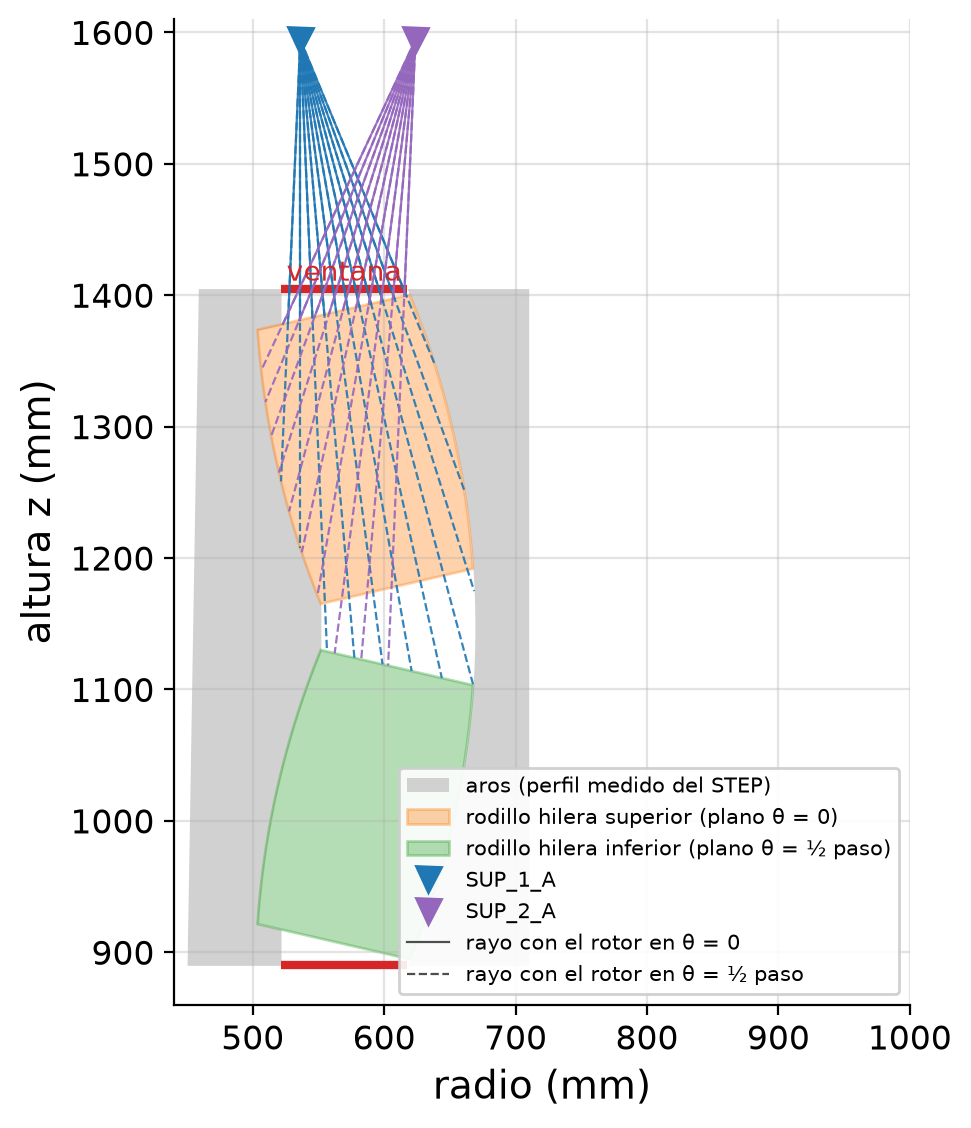
\includegraphics[width=0.55\textwidth]{asp_cavidad_seccion_rayos.png}
\caption[Sección del rodamiento armado con los rayos de las boquillas superiores]{Sección meridiana del rodamiento armado con los rayos de las dos boquillas superiores de un brazo, en dos posiciones del distribuidor. La hilera superior se ve en parte a través de la ventana entre aros y la inferior queda oculta. Geometría medida en el modelo del fabricante, sin jaula. Elaboración propia.}
\label{fig:anx-cavidad}
\end{figure}

\section{Impacto local de un chorro sobre el diámetro exterior}
\label{sec:anx-vof}

El modelo de fase discreta retiene la gota en el primer impacto y no resuelve la película que se forma en la pared. Para estimar la acción hidráulica local se simuló el impacto de la lámina de una boquilla lateral sobre el diámetro exterior con el método de volumen de fluido (VOF) de OpenFOAM v2606 (\texttt{interFoam}), en régimen laminar, con agua a 62~$^\circ$C y aire a 76,24 kPa. El caso es un corte bidimensional a través del espesor de la lámina, de 0,049 mm a 130 mm de la boquilla, con una velocidad de 27,5 m/s y medio dominio con plano de simetría. Se usaron cuatro mallas, con 5, 10, 20 y 40 celdas en el espesor de la lámina, y un número de Courant de 0,5. El orden de convergencia observado fue cercano a 2, la presión de estancamiento quedó dentro del 0,1\,\% de $\tfrac12\rho v^2$ y la fuerza local sobre la pared, un 0,5\,\% por encima de $\rho v^2 e_0$, lo que verifica el modelo frente a la teoría del chorro.

El empuje de la película a 0,33 mm del eje del impacto es de 17,0 N/m por lado, el 94\,\% del valor teórico, y el esfuerzo cortante en la pared en ese punto es de unos 2 kPa, con un pico de unos 9,5 kPa junto al eje (Figura~\ref{fig:anx-vof}). Esos valores suponen que la lámina llega intacta, por lo que son una cota superior. Un segundo caso, tridimensional, con el líquido representado como una mezcla diluida en el volumen del chorro, dio de 5 a 25 Pa, valores que crecen al refinar la malla: es una cota inferior. El esfuerzo cortante real queda entre ambas cotas y depende de si la lámina se rompe en gotas antes de llegar, lo que solo una medición de la huella puede aclarar. Por eso el esfuerzo cortante no se usó como criterio de evaluación del diseño.

\begin{figure}[htbp]
\centering
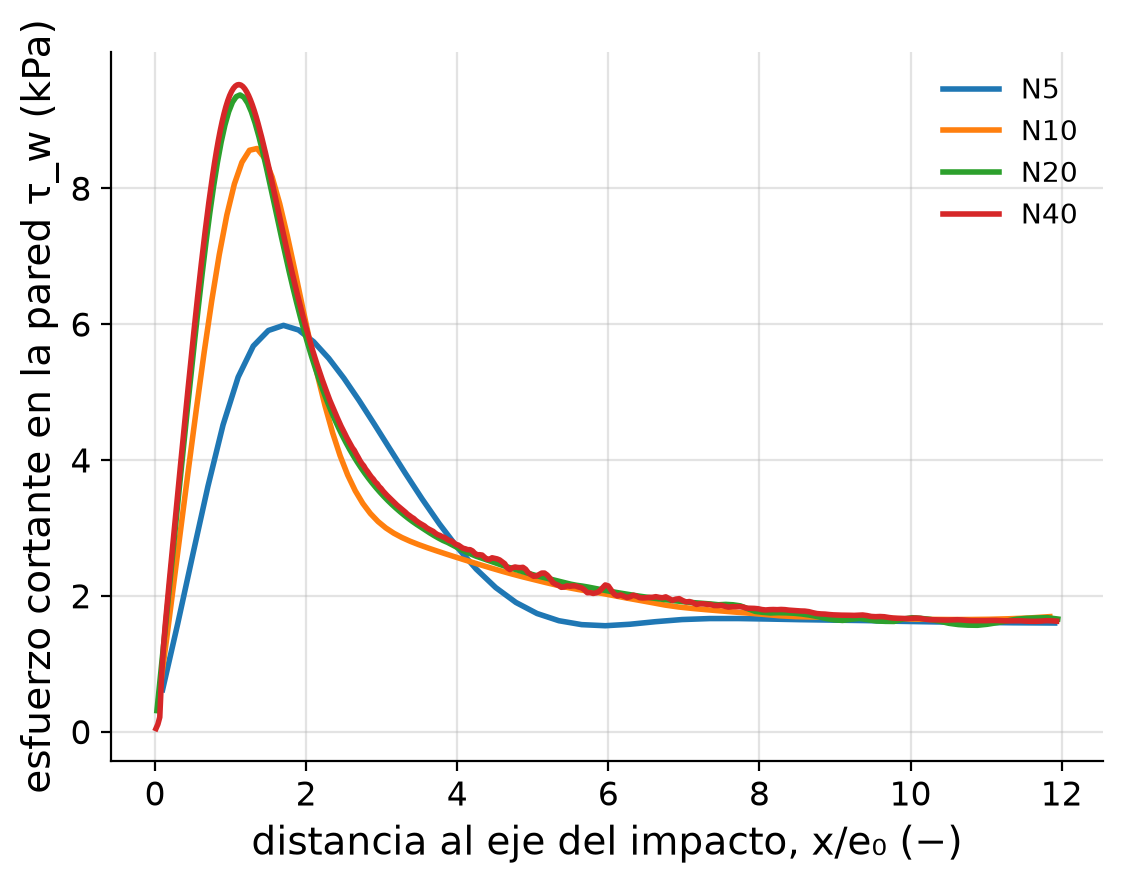
\includegraphics[width=0.58\textwidth]{asp_vof_cortante_od.png}
\caption[Esfuerzo cortante en la pared bajo la lámina de una boquilla lateral]{Esfuerzo cortante en la pared del diámetro exterior bajo la lámina de una boquilla lateral, con cuatro mallas (N5 a N40 celdas en el espesor de la lámina); la distancia al eje del impacto está dividida por el espesor de la lámina, $e_0$. Cota superior: lámina intacta. Elaboración propia, simulación en OpenFOAM v2606.}
\label{fig:anx-vof}
\end{figure}

\section{Correspondencia de nombres de cálculo y archivos}
La Tabla~\ref{tab:correspondencia-sap} relaciona los identificadores que aparecen en los archivos de respaldo con la denominación que se emplea en el informe.

\begingroup
\small\singlespacing
\setlength{\parskip}{0pt}
\setlength{\tabcolsep}{4pt}
\renewcommand{\arraystretch}{1.1}
\begin{longtable}{@{}>{\raggedright\arraybackslash}p{3.6cm}>{\raggedright\arraybackslash}p{\dimexpr(\textwidth-3.6cm-2\tabcolsep)/1\relax}@{}}
\caption{Correspondencia entre identificadores originales y denominaciones del informe}\label{tab:correspondencia-sap}\\
\toprule
\textbf{Denominación} & \textbf{Significado}\\

\midrule\endfirsthead
\caption[]{Correspondencia de identificadores y denominaciones (continuación)}\\
\toprule
\textbf{Denominación} & \textbf{Significado}\\

\midrule\endhead
\midrule\multicolumn{2}{r}{\textit{Continúa en la página siguiente.}}\\\endfoot
\bottomrule\endlastfoot
N3, N4, N5 & Bastidor con tres, cuatro o cinco apoyos sectoriales, respectivamente. Los apoyos reciben el rodamiento y son distintos de las cuatro ruedas del conjunto móvil.\\
R01 & Análisis estructural original realizado en SAP2000.\\
R03, R04, R05 & Revisiones mecánicas: reserva de masa y desarrollo de la integración. R05 identifica la revisión mecánica posterior al análisis original, no cinco apoyos.\\
R06, R06.1 & Integración de la mesa con el aplicador, los rieles y el drenaje (R06) y desarrollo de los centradores K2-M (R06.1). Configuración candidata vigente.\\
\texttt{LC\_G\_FRAME} & Peso propio del bastidor.\\
\texttt{LC\_G\_EXTERNAL} & Carga vertical externa aplicada en los apoyos sectoriales.\\
\texttt{SLS\_NOMINAL} & Combinación nominal de servicio: peso propio y carga externa con factor 1,00.\\
\texttt{SLS\_UNC\_125} & Servicio con carga externa amplificada por 1,25; peso propio con factor 1,00. Este factor no sustituye el factor mecánico 1,15.\\
\texttt{ULS\_1\_4D} & Combinación resistente: factor 1,40 sobre el peso propio y la carga externa, conforme a la Tabla~\ref{tab:combinaciones-r01}.\\
\texttt{DSTL1} & Identificador de la combinación resistente reportada para cuatro y cinco apoyos. Su equivalencia con la combinación del bastidor con tres apoyos no está demostrada.\\
\texttt{Frame}, \texttt{Frames} & Barra o elementos de barra del modelo.\\
\texttt{MatProp = Default} & Campo de asignación del material descrito en el apartado~\ref{sec:material-trazabilidad}. Para el bastidor W6×9 se consideró acero ASTM A36.\\
D/C & Razón demanda/capacidad; no es un factor de seguridad global.\\
PMM & Interacción de carga axial y flexión biaxial.\\
V5.2, I01 & Identificadores de la arquitectura y del cálculo de aspersión documentados.\\
PAD y liner & Apoyo sectorial del rodamiento y revestimiento de su superficie de contacto. En el informe se emplea «apoyos sectoriales».\\
K2-M, v5.7.3, v5.7.4 & Centrador de brazo pivotante de eje vertical derivado del concepto K2. La versión 5.7.3 es la vigente; la 5.7.4 es un estudio de refuerzo no adoptado.\\
U1, U2, U3 & Unidades de centrado: U1 y U3 son las referencias y U2 el empujador.\\
LOAD, WASH & Receptores del pasador de bloqueo en las estaciones de carga y de lavado.\\
E1, E2 & Etapas de limpieza: E1, con el rodamiento montado sobre la mesa, y E2, con sus elementos desmontados.\\
Libro I01 & Identificador documental de la hoja de cálculo hidráulico. En el texto se utiliza «hoja de cálculo hidráulico».\\
\end{longtable}

\endgroup

\chapter{PORTAFOLIO DE GESTIÓN DEL PROYECTO}
\label{anx:portafolio}

El portafolio del proyecto se conserva en \RepoProyecto, organizado en las carpetas siguientes:
\begin{itemize}
\item \enlacerepo{informe}: fuente \LaTeX{} y versiones en PDF de este informe;
\item \enlacerepo{cfd}: casos de ANSYS Fluent y OpenFOAM, guiones de posproceso y tablas de resultados del modelo de mojado;
\item \enlacerepo{hidraulica}: guiones y resultados de las redes de 19, 22 y 24 boquillas, y esquema hidráulico;
\item \enlacerepo{estructural}: modelos de SAP2000, modelos de CalculiX, cálculo de las uniones y libro mecánico del soporte;
\item \enlacerepo{cad}: modelo FreeCAD integrado, planos de SolidWorks y estudios complementarios;
\item \enlacerepo{gestion}: diagrama de Gantt, actas de las reuniones con el asesor y registro de decisiones de diseño.
\end{itemize}

El registro de decisiones guarda, para cada decisión, la fecha, las alternativas consideradas, la razón, la evidencia y su estado.

\section{Cronograma del proyecto}
\label{sec:cronograma-proyecto}

El segundo curso de Proyecto Final de Ingeniería se planificó en dieciséis semanas, del 10 de agosto al 29 de noviembre de 2026, en cuatro fases cerradas por un entregable: definición y contexto (primer entregable, 13 de septiembre), Caso Base y simulación (segundo entregable, 11 de octubre), iteración y rediseño (informe final, 22 de noviembre) y sustentación (29 de noviembre). La Figura~\ref{fig:gantt-1} presenta las fases 1 y 2 del cronograma, y la Figura~\ref{fig:gantt-2}, las fases 3 y 4.

\begin{figure}[p]
\centering
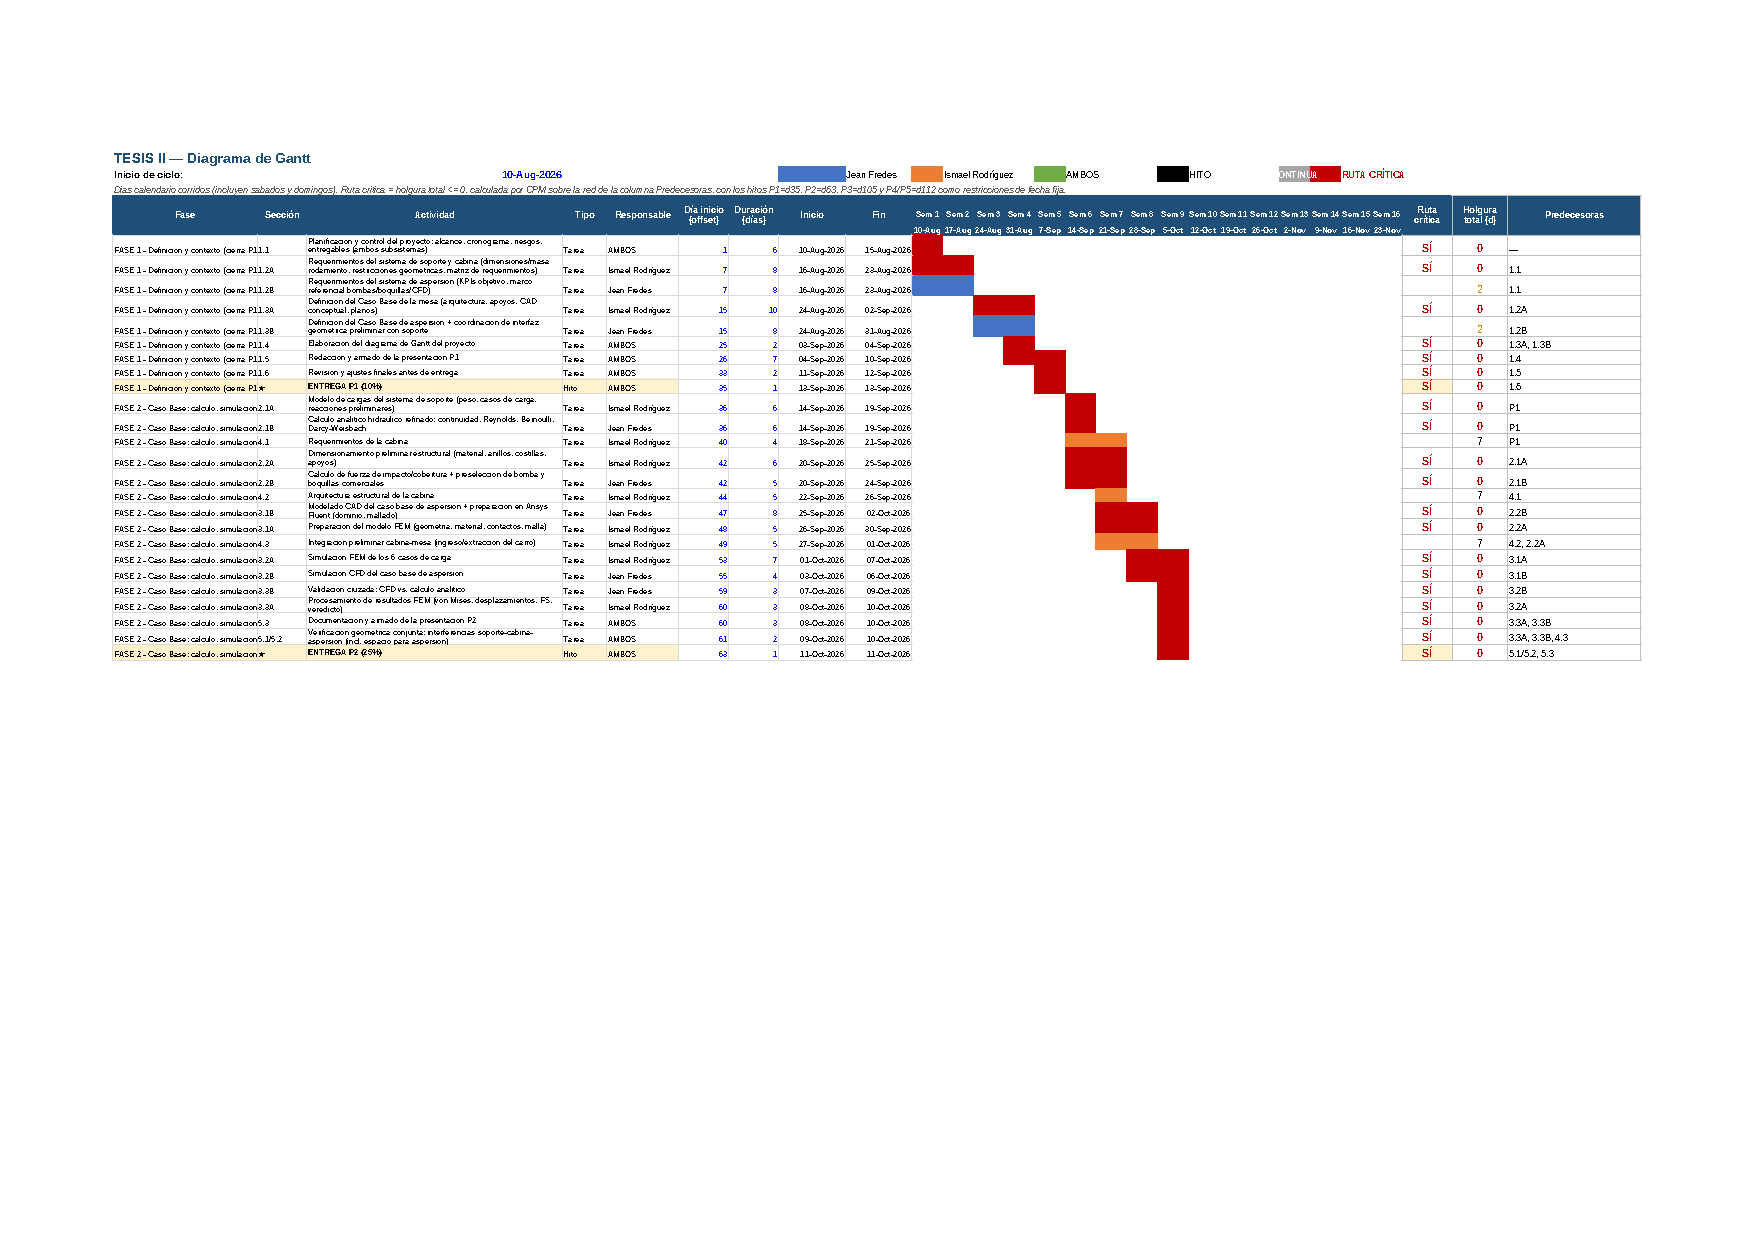
\includegraphics[page=1,trim=50bp 274bp 50bp 68bp,clip,angle=90,height=0.86\textheight]{anexos/Anexo_Gantt_TesisII.pdf}
\caption{Diagrama de Gantt del proyecto: fases 1 y 2 (10/08/2026--11/10/2026). Elaboración propia.}
\label{fig:gantt-1}
\end{figure}

\begin{figure}[p]
\centering
\includegraphics[page=2,trim=50bp 251bp 50bp 68bp,clip,angle=90,height=0.86\textheight]{anexos/Anexo_Gantt_TesisII.pdf}
\caption{Diagrama de Gantt del proyecto: fases 3 y 4 (12/10/2026--29/11/2026). Elaboración propia.}
\label{fig:gantt-2}
\end{figure}

\chapter{PROCESO ITERATIVO DE DISEÑO}
\label{anx:iteraciones}

Este anexo registra los cambios técnicos y paramétricos entre las revisiones del diseño, por subsistema, y respalda la Tabla~\ref{tab:iteraciones-resumen}; la Tabla~\ref{tab:anx-iteraciones} reúne el registro. Una revisión solo sustituye a la anterior en el aspecto que se comprobó; cada resultado se asigna a la geometría y al caso que lo produjeron. Las fechas corresponden a 2026.

\begingroup
\small\singlespacing
\setlength{\tabcolsep}{4pt}
\begin{longtable}{@{}>{\raggedright\arraybackslash}p{2.6cm}>{\raggedright\arraybackslash}p{\dimexpr(\textwidth-2.6cm-2.4cm-8\tabcolsep)*55/100\relax}>{\raggedright\arraybackslash}p{\dimexpr(\textwidth-2.6cm-2.4cm-8\tabcolsep)*45/100\relax}>{\raggedright\arraybackslash}p{2.4cm}@{}}
\caption{Registro de iteraciones por subsistema}\label{tab:anx-iteraciones}\\
\toprule
\textbf{Revisión} & \textbf{Cambio} & \textbf{Motivo} & \textbf{Estado}\\
\midrule\endfirsthead
\caption[]{Registro de iteraciones por subsistema (continuación)}\\
\toprule
\textbf{Revisión} & \textbf{Cambio} & \textbf{Motivo} & \textbf{Estado}\\
\midrule\endhead
\midrule\multicolumn{4}{r}{\textit{Continúa en la página siguiente.}}\\\endfoot
\bottomrule\endlastfoot
\multicolumn{4}{@{}l}{\textit{Estructura y mesa}}\\
Disposición inicial (julio) & Mesa abierta conceptual & Arranque del proyecto & Histórica\\
Modelos de cabina (agosto) & Mesa circular con aros, nervios y brazos de rueda en voladizo & Evolución de la arquitectura de la cabina & Superada\\
Modelos de línea (28--30/08) & Bastidores de tres, cuatro y cinco apoyos sectoriales con el mismo perfil & Comparar topologías para el análisis estructural & Superada\\
Análisis estructural (31/08--04/09) & Bastidor de tres apoyos en W6$\times$9: D/C de 0,28 & Cribado estructural & Ejecutado\\
Revisiones mecánicas 1--3 (05--06/09) & Cabina y puerta, rieles A45, recorrido de 3320 mm, masa de 3500 kg, ruedas SPKVS 200K; horquilla de 68 a 80 mm; reacciones en los apoyos por equilibrio & Desarrollo mecánico y revisión independiente & Superadas\\
Revisión 4 (07--08/09) & Bloqueo unido al bastidor; centrador retraído; eje de rueda de 35 mm & Encargo de revisión mecánica & Superada\\
Revisión 5 (08/09) & Colocación $\leq5$ mm; topes y manillar conectados; envolvente del riel & Cierre de los hallazgos de la revisión 4 & Vigente (mesa)\\
Integración (24/09 en adelante) & Soportes de riel reubicados (12 por riel); piso de drenaje fijo con pendiente, sumidero y cesta; estados de carga y lavado & Choques del centrador con la jamba, de los soportes con el muro y del drenaje con los rieles & Candidato\\
Travesaño adicional (29/09) & Propuesto y retirado & Mejoraba la deformación, pero quedaba bajo la lanza y dependía de uniones a momento & Retirado\\
Rueda y riel (27--29/10) & Fuerza lateral de guiado de 6,51 kN; retención axial de las ruedas; se compararon las ruedas de 200 y 250 mm & La versión anterior comparaba la carga última con la capacidad de rodadura & Se mantiene la de 200 mm\\
Traslado (29/10) & Doble cadena bajo la mesa con volante en lugar del empuje manual & Empuje de 325 a 837 N y frenado de 565 N & Vigente\\
Uniones del bastidor (02/11) & Alas a tope con penetración completa, alma con filete de 3 mm, rigidizador de 6 mm y tapas en las esquinas & Las uniones estaban especificadas pero no diseñadas & Vigente\\
Pedestales del riel (02--03/11) & Pedestal de inoxidable 304 con 4 anclajes adhesivos M16 & Levantamiento de 3,78 kN, guiado y tensor de las cadenas & Vigente\\
Topes de retención (03/11) & Cartelas a 60$^\circ$ y 300$^\circ$ y chapa de asiento a 190$^\circ$ & La base supuesta del tope no existía en el CAD: cordón con D/C 3,97 & Vigente\\
\multicolumn{4}{@{}l}{\textit{Centradores}}\\
Módulos de carro radial (revisión 5) & Centradores con carro y guía & Centrado de la revisión 5 & Superados: atravesaban perfiles e invadían el rodamiento\\
Selección de conceptos & Carro radial, brazo pivotante y leva excéntrica; puntajes de 2,675, 3,250 y 3,075 & Diez condiciones excluyentes y matriz ponderada & Brazo pivotante seleccionado\\
Versiones 5 a 5.7.1 & Desarrollo del brazo pivotante, con dos referencias y un empujador & Modelado, barridos y elementos finitos & Superadas\\
Versión 5.7.2b & Amarre transversal de las referencias con dos pernos M12 & Flexibilidad de la mordaza & Superada\\
Versión 5.7.3 & Brazo del empujador de 67,15 mm (+2 mm de recorrido) & Captura de 4,69 mm, menor que 5 mm, en el peor caso & Superada\\
Versión 5.7.4 (20/10) & Placa del soporte del empujador de 20 a 28 mm, con soldaduras a tope de penetración completa & Tensiones de 190--246 MPa en la placa de 20 mm & Vigente\\
Amarre del empujador (27/10) & Dos pernos pasantes M12 por el alma de la viga longitudinal & El apriete anterior no tenía un camino de reacción cerrado & Vigente\\
Centrado por fuerza (02/11) & Ajuste H7/g6 y límite de 1,95 kN a la fuerza final; sin cono de indexado & Error de 6,10 mm en la envolvente; el 70\,\% era deformación elástica & Vigente\\
\multicolumn{4}{@{}l}{\textit{Aspersión}}\\
Modelos de cabina (agosto) & Distribuidor en U, brazos dobles, brazo en L y cabezal sobre monorriel & Cobertura geométrica por trazado de rayos & Superados\\
Auditoría hidráulica (01/09) & Arquitecturas del cabezal sin seleccionar & Faltaban datos de proceso & Superada\\
U giratoria (12/09) & La U superior giratoria sustituye al cabezal sobre monorriel & Nuevo planteamiento del aplicador & Vigente\\
Caso base (16/09) & 19 boquillas, 1,7 rpm, agua a 62~$^\circ$C, 174 L/min & Memoria hidráulica del caso base & Superado por la red de 22\\
Lanza corta (18/09) & Lanza a 25$^\circ$ en lugar de 28$^\circ$; dos salidas inferiores exteriores; 22 boquillas; traslado solo con el aplicador a 0$^\circ$ & Con 28$^\circ$ quedaban 90 de 18\,720 puntos sin acceso & Vigente, salvo las salidas inferiores\\
Cierre preliminar (18/09) & Manguera en lazo, toma fija reubicada, válvulas, purgas y seguros; boquilla comercial candidata & Cierre de ingeniería preliminar del aplicador & Vigente\\
Red de 22 boquillas & 202,59 L/min y 52,56 m; toma crítica en la lanza & Geometría de la lanza corta & Superada por la de 24\\
Par inferior de abanico estrecho (08/10) & Boquilla inferior exterior a 15$^\circ$ y una adicional a 10,7$^\circ$ en cada brazo: 24 boquillas, 221,07 L/min y 53,39 m & La cara inferior recibía cuatro veces menos dosis; la boquilla anterior mojaba la base del diámetro exterior & Vigente\\
U desmontable (02/11) & Dos juntas bridadas DN50 a 300 mm del eje, sin válvulas de ramal; brazos iguales & Las válvulas de ramal no tenían función documentada & Vigente\\
Rotor, eje y cubo (02/11) & Masa medida en el CAD: 231 kg; cubo soldado al eje y mecanizado con él & La envolvente de 180 kg no cubría el rotor real & Vigente\\
Tolerancias de las coplas (03/11) & $\pm2$ mm y $\pm1^\circ$ en las coplas; $\pm1$ mm y $\pm0{,}5^\circ$ en el bloque inferior & Trazado de rayos con 240 perturbaciones & Vigente\\
Soporte superior (27/10 y 03/11) & Marco propio dentro de los muros; postes SHS80$\times$4 y vigas RHS150$\times$100$\times$3 & La cabina no basta como estructura; el criterio anterior no era funcional & Vigente: de 360 a 247 kg\\
\multicolumn{4}{@{}l}{\textit{Simulación del mojado}}\\
Planificación (julio a 18/09) & De una boquilla aislada a un modelo de gotas de las 6 boquillas del agujero & Definir el fenómeno relevante & Superada\\
Agujero en OpenFOAM (19--21/09) & Dos ramas de cálculo; la oficial, con acoplamiento en dos vías y 430\,294 celdas & Primer modelo del mojado & Antecedente\\
Caso puente en Fluent (26--30/09) & Agujero repetido en Fluent: $-0{,}27$\,\% en dosis media & Ampliar el dominio a 22 boquillas dentro del límite de la licencia & Ejecutado\\
Caso Base de 22 boquillas (30/09--02/10) & Cuatro superficies con los obstáculos del soporte; verificación de malla, paso de tiempo, dominio y parcelas & Configuración vigente en esa fecha & Ejecutado\\
Variantes del diámetro exterior & Lateral 1 inclinada $-4^\circ$; segunda boquilla superior 15 mm hacia fuera & Franja seca de 2 mm en el diámetro exterior & Lateral inclinada incorporada (26/10); superior desplazada no incorporada\\
Configuración propuesta (25--26/10) & 24 boquillas con los dos brazos explícitos; tres mallas con Courant de gota constante y dos números de parcelas & Comprobar el par inferior con el CFD & Ejecutado\\
\end{longtable}
\endgroup

La Tabla~\ref{tab:comparacion-apoyos} compara los bastidores de tres, cuatro y cinco apoyos con la misma carga externa total, repartida por igual entre sus apoyos. Se mantuvo el de tres apoyos por masa y simplicidad, a cambio de una flecha 63\,\% mayor que la del de cinco, todavía inferior a los límites en evaluación.

\begin{table}[htbp]
\centering\small\singlespacing
\caption{Resultados de las alternativas de bastidor}
\label{tab:comparacion-apoyos}
\begin{tabular}{lrrr}
\toprule
\textbf{Magnitud} & \textbf{Tres apoyos} & \textbf{Cuatro apoyos} & \textbf{Cinco apoyos}\\
\midrule
Carga externa por apoyo (N) & 9948 & 7461 & 5968,8\\
Elementos de barra & 20 & 24 & 28\\
Masa de perfiles (kg) & 168,1 & 188,5 & 180,8\\
Máximo $|U_3|$ nominal (mm) & 1,353 & 1,441 & 0,953\\
Flecha relativa nodal (mm) & 1,236 & 1,415 & 0,757\\
Desnivel entre apoyos (mm) & 0,294 & 0,410 & 0,220\\
D/C publicado & 0,277 & 0,278* & 0,175*\\
\bottomrule
\end{tabular}
\par\smallskip\footnotesize
*Combinación resistente cuya equivalencia con la del bastidor de tres apoyos no está demostrada; no se usa para ordenar las alternativas.
\end{table}


% anexo_i_reuniones_skf.tex se conserva sin incluir; el Anexo 7 (portafolio) contiene solo el repositorio y el cronograma.


\end{document}
